\documentclass[compress]{beamer}
\usetheme{Warsaw}
\useoutertheme{split}

%%%%%%%%%%%%%%%%%%%%%%%%%%%%%%%%%%%%%%%%%%%%%%%%%%%%%%%%%%%%%%%
% Improvement on the default split theme : added line numbers %
%%%%%%%%%%%%%%%%%%%%%%%%%%%%%%%%%%%%%%%%%%%%%%%%%%%%%%%%%%%%%%%

%%%%%%%%%%%%%%%
% Main colors %
%%%%%%%%%%%%%%%

\setbeamercolor{frametitle}{fg=white}
\setbeamercolor{frametitle right}{fg=white}
\setbeamercolor{structure}{fg=beamer@blendedblue} % this should be the default anyway, but make sure, since we change it between basic/advanced slides
\setbeamercolor{goodpractice head}{fg=white,bg=orange!85!black}
\setbeamercolor{goodpractice body}{fg=black,bg=orange!25}

%%%%%%%%%%%%%%%%%%%%%%%%%
% headline and footline %
%%%%%%%%%%%%%%%%%%%%%%%%%

\defbeamertemplate*{footline}{mysplit theme}
{%
  \leavevmode%
  \hbox{\begin{beamercolorbox}[wd=.5\paperwidth,ht=2.5ex,dp=1.125ex,leftskip=.3cm plus1fill,rightskip=.3cm]{author in head/foot}%
    \usebeamerfont{author in head/foot}\insertshortauthor%
  \end{beamercolorbox}%
  \begin{beamercolorbox}[wd=.4\paperwidth,ht=2.5ex,dp=1.125ex,leftskip=.3cm,rightskip=.3cm plus1fil]{title in head/foot}%
    \usebeamerfont{title in head/foot}\insertshorttitle%
  \end{beamercolorbox}}%
    \begin{beamercolorbox}[wd=.1\paperwidth,ht=2.5ex,dp=1.125ex,leftskip=.1cm plus1fill,rightskip=.1cm]{date in head/foot}%
      \usebeamerfont{date in head/foot} \insertframenumber{} / \inserttotalframenumber%
    \end{beamercolorbox}%
  \vskip0pt%
}

\defbeamertemplate*{headline}{mysplit theme}
{%
  \leavevmode%
  \begin{beamercolorbox}[wd=.4\paperwidth,ht=2.5ex,dp=1.125ex]{section in head/foot}%
    \insertsectionnavigationhorizontal{.4\paperwidth}{\hskip0pt plus1filll}{}%
  \end{beamercolorbox}%
  \begin{beamercolorbox}[wd=.6\paperwidth,ht=2.5ex,dp=1.125ex]{subsection in head/foot}%
    \insertsubsectionnavigationhorizontal{.6\paperwidth}{}{\hskip0pt plus1filll}%
  \end{beamercolorbox}%
}

%%%%%%%%%%%%
% packages %
%%%%%%%%%%%%

\usepackage{fontawesome}
\usepackage{morewrites}
\usepackage[utf8]{inputenc}
\usepackage{newunicodechar}
\usepackage{scontents}
\makeatletter
\let\verbatimsc\@undefined
\let\endverbatimsc\@undefined
\makeatother
\usepackage{minted}
\newminted{tex}{linenos}
\newenvironment{verbatimsc}
               {\VerbatimEnvironment
                 \begin{minted}[linenos,escapeinside=||]{cpp}}
               {\end{minted}}
\newcommand\highlightCppCode[2]{
  \renewenvironment{verbatimsc}
                   {\VerbatimEnvironment
                     \begin{minted}[linenos,highlightlines={#1},escapeinside=||]{cpp}}
                   {\end{minted}}
  \typestored{#2}
}
\newminted{cpp}{gobble=4,linenos}
\newminted{shell-session}{gobble=4}
\newminted[makefile]{shell-session}{gobble=4}
\newminted{python}{linenos=true,gobble=4}

\usepackage{fancyvrb}
\newcommand*{\fvtextcolor}[2]{\textcolor{#1}{#2}}

\usepackage{pgf}
\usepackage{pgffor}
\usepackage{tikz}
\usetikzlibrary{arrows,arrows.meta,automata,positioning,snakes,shapes}

\usepackage{tcolorbox}

\usepackage[framemethod=TikZ]{mdframed}
\mdfdefinestyle{simplebox}{roundcorner=4pt,linewidth=0,backgroundcolor=blue!50!black,fontcolor=white}

\usepackage{multicol}
\usepackage{tikz-uml}

\usepackage{booktabs}
\usepackage{comment}
\usepackage{totcount}

% Use C++Course.cut for output so it's cleaned by latexmk
\def\DefaultCutFileName{\def\CommentCutFile{\jobname.cut}}
\DefaultCutFileName

%%%%%%%%%%%%%%%%%%%
% useful commands %
%%%%%%%%%%%%%%%%%%%
\newcommand{\cpp}{C$^{++}$}
\newcommand{\deprecated}{\textcolor{red}{\bf Deprecated}}
\newcommand{\removed}{\textcolor{red}{\bf Removed}}


%%%%%%%%%%%%%%%%%%%%%%%%%%%%%%%%%%%%%%%%%%%%%%%%%
% boxes with good practices                     %
% Use \begin{goodpractice}{Title} to create one %
%%%%%%%%%%%%%%%%%%%%%%%%%%%%%%%%%%%%%%%%%%%%%%%%%
\makeatletter
\newcommand\listofgoodpractices{%
  \addtocontents{lgp}{\end{enumerate}}
  \scriptsize
  \begin{multicols}{2}
    \@starttoc{lgp}%
  \end{multicols}
}
\AtBeginDocument{ \addtocontents{lgp}{\begin{enumerate} } }

\newcounter{gp@counter}
\def\gp@lasttitle{None}

\newenvironment{goodpracticeWithShortcut}[2]
{%
  % Generate an entry in the index of good practices. In case of slide overlays, we only generate
  % an entry for the first slide of the overlay set by saving the last title of the
  % good practice box.
  \ifthenelse{\equal{\gp@lasttitle}{#1}}{}{%
    \hypertarget<1>{goodpractice.\thegp@counter}{}
    \addtocontents{lgp}{\protect\item \protect\hyperlink{goodpractice.\thegp@counter}{#2\protect\hfill\insertframenumber}}
    \stepcounter{gp@counter}
    \gdef\gp@lasttitle{#1}
  }
  % The box that shows up on the slide
  \begin{beamerboxesrounded}[upper=goodpractice head,lower=goodpractice body,shadow=true]{Good practice: #1}
}%
{%
  \end{beamerboxesrounded}
}
\newenvironment{goodpractice}[1]
{%
  \begin{goodpracticeWithShortcut}{#1}{#1}
}%
{%
  \end{goodpracticeWithShortcut}
}

%%%%%%%%%%%%%%%%%%%%%%%%%%%%%%%%%%%%%%%%%%%%%%%%%
% boxes with exercises                          %
% Use \begin{exercise}{Title} to create one     %
%%%%%%%%%%%%%%%%%%%%%%%%%%%%%%%%%%%%%%%%%%%%%%%%%
\newcommand\listofexercises{%
  \addtocontents{lex}{\end{enumerate}}
  \scriptsize
  \begin{multicols}{3}
    \@starttoc{lex}%
  \end{multicols}
}
\AtBeginDocument{ \addtocontents{lex}{\begin{enumerate} } }

\newcounter{ex@counter}
\regtotcounter{ex@counter}

\newenvironment{exerciseWithShortcut}[2]
{%
  \hypertarget<1>{exercise.\theex@counter}{}
  \addtocontents{lex}{\protect\item \protect\hyperlink{exercise.\theex@counter}{#2\protect\hfill\insertframenumber}}
  \stepcounter{ex@counter}
  % The box that shows up on the slide
  \begin{alertblock}{Exercise: #1}
}%
{%
  \end{alertblock}
}
\newenvironment{exercise}[1]
{%
  \begin{exerciseWithShortcut}{#1}{#1}
}%
{%
  \end{exerciseWithShortcut}
}

%%%%%%%%%%%%%%%%%%%%%%%%%%%%%%%
% frametitle with C++ version %
%%%%%%%%%%%%%%%%%%%%%%%%%%%%%%%
% Use as \frametitlecpp[14]{Title}
\newcommand\frametitlecpp[2][98]{
  \frametitle{#2 \hfill \cpp#1}
}

%%%%%%%%%%%%%%%%%%%%%%%%%%%%%%%%%%%%%%%%
% easy links to godbolt and cppinsight %
%%%%%%%%%%%%%%%%%%%%%%%%%%%%%%%%%%%%%%%%
\newcommand\listofgodbolt{%
  \addtocontents{lgb}{\end{enumerate}}
  \scriptsize
  \begin{multicols}{2}
    \@starttoc{lgb}%
  \end{multicols}
}
\AtBeginDocument{ \addtocontents{lgb}{\begin{enumerate} } }

\newcounter{gb@counter}
\regtotcounter{gb@counter}
\resetcounteronoverlays{gb@counter}
\newcommand*{\overlaynumber}{\number\beamer@slideinframe}

% Use as \godboltLink{url}
\newcommand\godboltLink[2]{%
  \href{#1}{\color{blue!50!white} godbolt}%
  \ifnum \overlaynumber=1%
    \hypertarget<1>{godbolt.\thegb@counter}{}
    \addtocontents{lgb}{\protect\item \protect\hyperlink{godbolt.\thegb@counter}{#2 - \href{#1}{godbolt}\protect\hfill\insertframenumber}}%
    \stepcounter{gb@counter}%
  \fi
}

% Use as \begin{exampleblockGB}{<Title of box on slide>}{<godbolt link>}{<title in index>}
\newenvironment{exampleblockGB}[3]
{%
  \begin{exampleblock}{#1 - \godboltLink{#2}{#3}}
}%
{%
  \end{exampleblock}
}

% Use as \cppinsightLink{url}
\newcommand\cppinsightLink[1]{%
  \href{#1}{\color{blue!50!white} cppinsight}%
}
% Use as \cppinsightLink{url}
\newcommand\cpprefLink[1]{%
  \href{#1}{\color{blue!50!white} cppreference}%
}

% Use as \youtubechannel{channelname}
\newcommand\youtubechannel[1]{%
  \mbox{\href{https://www.youtube.com/c/#1}{\color{red}\faYoutubePlay\ #1}}%
}

% Use as \youtubeuser{username}
\newcommand\youtubeuser[1]{%
  \mbox{\href{https://www.youtube.com/user/#1}{\color{red}\faYoutubePlay\ #1}}%
}

\makeatother

%%%%%%%%%%%%%%%%%%%%%%%%%%%%%%%
% easy class diagrams in tikz %
%%%%%%%%%%%%%%%%%%%%%%%%%%%%%%%

\newcommand\classbox[3][]{
  \def\temp{#3}
  \ifx\temp\empty
    \draw[thick] node (#2) [#1]
         [rectangle,rounded corners,draw] {#2};
  \else
    \draw[thick] node (#2) [#1]
         [rectangle,rounded corners,draw] {
      \begin{tabular}{l}
        \multicolumn{1}{c}{#2} \\
        \hline
        #3
      \end{tabular}
    };
  \fi
}

%%%%%%%%%%%%%%%%%%%%%%%%%%%%%%%%%%%%%%
% easy memory stack diagrams in tikz %
%%%%%%%%%%%%%%%%%%%%%%%%%%%%%%%%%%%%%%

\newcounter{memorystackindex}

\pgfkeys{
  memorystack/.is family,
  memorystack,
  size x/.initial=4cm,
  size y/.initial=.5cm,
  word size/.initial=4,
  block size/.initial=1,
  nb blocks/.initial=8,
  base address/.initial=12288,
  color/.initial=black,
  addresses/.initial=1
}

\makeatletter

\newcommand\memorystackset[1]{\pgfkeys{memorystack,#1}}
\newcommand\memorystack[1][]{
  \memorystackset{#1,
    size x/.get=\stacksizex,
    size y/.get=\stacksizey,
    word size/.get=\stackwordsize,
    block size/.get=\blocksize,
    nb blocks/.get=\stacknbblocks,
    base address/.get=\stackbaseaddr,
    color/.get=\stackcolor,
    addresses/.get=\displayaddrs
  }
  \draw[thick,\stackcolor,text=white] node (title)
        at (\stacksizex/2, \stacknbblocks*\stacksizey+.5cm)
        [rectangle,rounded corners,fill=blue!50!black] {Memory layout};
  \setcounter{memorystackindex}{1}
  \draw[thick,\stackcolor] (0,0) rectangle (\stacksizex,\stacknbblocks*\stacksizey);
  \pgfmathsetmacro{\nbbars}{\stacknbblocks-1}
  \pgfmathtruncatemacro\nbbarstrunc{\nbbars}
  \ifnum\nbbarstrunc>0
    \foreach \n in {1,...,\nbbarstrunc} {
      \draw[\stackcolor!70] (0,\n*\stacksizey) -- +(\stacksizex,0);
    }
  \fi
  \foreach \n in {1,...,\stacknbblocks} {
    \foreach \p in {1,...,\stackwordsize} {
      \draw node (stack\n-\p)
            at (\stacksizex/\stackwordsize*\p-\stacksizex/\stackwordsize/2,\n*\stacksizey-\stacksizey/2)
            [rectangle,minimum width=\stacksizex,minimum height=\stacksizey] {};
    }
    \ifnum1=\displayaddrs\relax
      \pgfmathparse{(\n-1)*\blocksize*\stackwordsize+\stackbaseaddr}
      \pgfmathtruncatemacro\addressdec{\pgfmathresult}
      \pgfmathdectoBase\hexversion{\addressdec}{16}
      \draw node at (\stacksizex,\n*\stacksizey-\stacksizey/2) [right=2pt]
            {0x\hexversion};
    \fi
  }
  \pgfmathsetmacro{\nbseps}{\stackwordsize-1}
  \pgfmathtruncatemacro\nbsepstrunc{\nbseps}
  \ifnum\nbsepstrunc>0
    \foreach \n in {1,...,\nbsepstrunc} {
      \draw[\stackcolor!10] (\stacksizex/\stackwordsize*\n,0) -- +(0,\stacknbblocks*\stacksizey);
    }
  \fi
}

\newcommand\memorypushvalue[3]{
  \draw node at (stack#1-#2) {#3};
}

\newcommand\memorypushwidevalue[1]{
  \memorystackset{
    size x/.get=\stacksizex,
    size y/.get=\stacksizey,
  }
  \draw node (content) at (\stacksizex/2,\value{memorystackindex}*\stacksizey-\stacksizey/2) {#1};
  \draw[\stackcolor!80,->] (content) -- (.2cm,\value{memorystackindex}*\stacksizey-\stacksizey/2);
  \draw[\stackcolor!80,->] (content) -- (\stacksizex-.2cm,\value{memorystackindex}*\stacksizey-\stacksizey/2);
  \addtocounter{memorystackindex}{1}
}

\newcommand\memorypushhalfvalue[1]{
  \memorystackset{
    size x/.get=\stacksizex,
    size y/.get=\stacksizey,
  }
  \draw node (content) at (\stacksizex/4,\value{memorystackindex}*\stacksizey-\stacksizey/2) {#1};
  \draw[\stackcolor!80,->] (content) -- (.2cm,\value{memorystackindex}*\stacksizey-\stacksizey/2);
  \draw[\stackcolor!80,->] (content) -- (\stacksizex/2-.2cm,\value{memorystackindex}*\stacksizey-\stacksizey/2);
  \addtocounter{memorystackindex}{1}
}

\newcounter{localcount}
\newcommand\memorypush[1]{
  \memorystackset{
    word size/.get=\stackwordsize,
    nb blocks/.get=\stacknbblocks
  }
  \count@=0
  \setcounter{localcount}{1}
  \@for\v:=#1\do{
    \ifnum\count@<\stackwordsize
      \advance\count@ 1
      \memorypushvalue{\arabic{memorystackindex}}{\arabic{localcount}}{\v}
    \fi
    \addtocounter{localcount}{1}
  }
  \addtocounter{memorystackindex}{1}
}

\newcommand\memorypushpointer[2][]{
  \memorystackset{
    word size/.get=\stackwordsize,
    base address/.get=\stackbaseaddr,
    block size/.get=\blocksize,
  }
  \pgfmathparse{(#2-1)*\stackwordsize*\blocksize+\stackbaseaddr}
  \pgfmathtruncatemacro\addressdec{\pgfmathresult}
  \pgfmathdectoBase\hexaddress{\addressdec}{16}
  \memorypushvalue{\arabic{memorystackindex}}{1}{#1 0x\hexaddress}
  \draw[\stackcolor!80,->] (stack\arabic{memorystackindex}-1.west) .. controls +(left:1) and +(left:1) .. (stack#2-1.west);
  \addtocounter{memorystackindex}{1}
}

\newcommand\memorystruct[3]{
  \memorystackset{
    size y/.get=\stacksizey
  }
  \draw[snake=brace,thick] (-2pt,#1*\stacksizey-\stacksizey) -- (-2pt,#2*\stacksizey)
    node [midway, above, sloped] {#3};
}

\newcommand\memorygoto[1]{
  \setcounter{memorystackindex}{#1}
}
\makeatother

%%%%%%%%%%%%%%%%%%
% Document setup %
%%%%%%%%%%%%%%%%%%

\title{HEP \cpp course}
\author[B. Gruber, S. Hageboeck, S. Ponce]{B. Gruber, S. Hageboeck, S. Ponce \\ \texttt{sebastien.ponce@cern.ch}}
\institute{CERN}
\date{\today}
\pgfdeclareimage[height=0.5cm]{cernlogo}{CERN-logo.jpg}
\logo{\pgfuseimage{cernlogo}}

\AtBeginSection[] {
  \begin{frame}<beamer>
    \frametitle{\insertsection}
    \begin{multicols}{2}
      \tableofcontents[sectionstyle=show/shaded,subsectionstyle=show/show/hide]
    \end{multicols}
  \end{frame}
}

\AtBeginSubsection[] {
  \begin{frame}<beamer>
    \frametitle{\insertsubsection}
    \tableofcontents[sectionstyle=show/hide,subsectionstyle=show/shaded/hide]
  \end{frame}
}

\hypersetup{
  colorlinks=true,
  allcolors=.,
  urlcolor={blue!80!white}
}


% setup for the basic/advanced course switch
% create a new latex if called basic (false by default)
\newif\ifbasic

% There are three ways to switch to the basic course:
% 1. Uncomment the line below. Disadvantage: git diff won't be empty
%\basictrue
% 2. Tell it to the Makefile.
%  2.1 Invoke "make essentials"
%  2.2 export HEPCPP_ESSENTIALS=1
%      make <target>
\ifdefined\makebasic
  \basictrue
\fi
% 3. Create a file named ./buildbasic
\IfFileExists{./buildbasic}{\basictrue}

% create a comment environment advanced. depending on the value of basic, we exclude or include it.
\ifbasic
  \excludecomment{advanced}
\else
  % advanced slides have a different structure color
  \specialcomment{advanced}{
    \setbeamercolor{structure}{fg=beamer@blendedblue!40!violet}
    \isAdvancedSlidetrue
  }{
    \setbeamercolor{structure}{fg=beamer@blendedblue}
    \isAdvancedSlidefalse
  }
\fi

\newunicodechar{σ}{$\sigma$}
\newunicodechar{µ}{$\mu$}

\begin{document}

\showboxdepth=\maxdimen
\showboxbreadth=\maxdimen

\begin{frame}
  \titlepage
\end{frame}

\begin{frame}
  \frametitle{Foreword}
  \begin{block}{What this course is not}
    \begin{itemize}
    \item It is not for absolute beginners
    \item It is not for experts
    \item It is not complete at all (would need 3 weeks...)
      \begin{itemize}
      \item although it is already too long for the time we have
      \item \inserttotalframenumber{} slides, \insertpresentationendpage{} pages, \total{ex@counter} exercises...
      \end{itemize}
    \end{itemize}
  \end{block}
  \begin{block}{How I see it}
    \begin{description}
    \item[Adaptative] pick what you want
    \item[Interactive] tell me what to skip/insist on
    \item[Practical] let's spend time on real code
    \end{description}
  \end{block}
  \begin{block}{Where to find latest version ?}
    \begin{itemize}
    \item full sources at \href{https://github.com/hsf-training/cpluspluscourse}{github.com/hsf-training/cpluspluscourse}
    \item latest pdf on
    \ifbasic
      \href{https://github.com/hsf-training/cpluspluscourse/raw/download/talk/C++Course\_essentials.pdf}{GitHub}
    \else
      \href{https://github.com/hsf-training/cpluspluscourse/raw/download/talk/C++Course\_full.pdf}{GitHub}
    \fi
    \end{itemize}
  \end{block}
\end{frame}


\begin{frame}
  \frametitle{More courses}
  \begin{block}{The HSF Software Training Center}
    A set of course modules on more software engineering aspects prepared from within the HEP community
    \begin{itemize}
      \item Unix shell
      \item Python
      \item Version control (git, gitlab, github)
      \item ...
    \end{itemize}
    {\small \url{https://hepsoftwarefoundation.org/training/curriculum.html}}
  \end{block}

\end{frame}

\begin{frame}
  \frametitle{Outline}
  \begin{multicols}{2}
    \tableofcontents[sectionstyle=show,subsectionstyle=hide]
  \end{multicols}
\end{frame}

\begin{frame}
  \frametitle{Detailed outline}
  %\vspace{-0.5cm}
  \begin{tiny}
    \begin{multicols}{3}
      \tableofcontents[sectionstyle=show,subsectionstyle=show]
    \end{multicols}
  \end{tiny}
\end{frame}

\section[Intro]{History and goals}
\subsection[Hist]{History}

\begin{frame}
  \frametitle{C/\cpp origins}
  \begin{minipage}{0.4\linewidth}
    \tikzstyle{old}=[ellipse,draw=black,fill=orange!30,thick,inner sep=2pt]
    \tikzstyle{new}=[rectangle,draw=black,fill=green!50,thick,inner sep=2pt]
    \tikzstyle{direct}=[<-,semithick]
    \tikzstyle{transverse}=[<-,dotted,semithick]
    \begin{tikzpicture}[->, node distance=.75cm, font=\tiny, scale=0.8, every node/.style={scale=0.8}]
      \node[old] (Simula)      {Simula};
      \node[left of=Simula,node distance=1.5cm] {1967};
      \node[old] (BCPL) [right of=Simula, node distance=2cm] {BCPL};
      \node[old] (B) [below of=BCPL] {B}
      edge[transverse] (BCPL);
      \node[old] (KandRC) [below of=B] {K and R C}
      edge[transverse] (B);
      \node[left of=KandRC,node distance=3.5cm] {1978};
      \node[old] (ClassicC) [below of=KandRC] {Classic C}
      edge[direct] (KandRC);
      \node[old] (CwithClasses) [below of=Simula,node distance=3cm] {C with Classes}
      edge[transverse] (Simula)
      edge[transverse] (BCPL)
      edge[direct] (ClassicC);
      \node[left of=CwithClasses,node distance=1.5cm] {1980};
      \node[old] (EarlyC++) [below of=CwithClasses] {Early \cpp}
      edge[direct] (CwithClasses);
      \node[left of=EarlyC++,node distance=1.5cm] {1985};
      \node[old] (C89) [below of=ClassicC,node distance=2.25cm] {C89}
      edge[direct] (ClassicC)
      edge[transverse] (CwithClasses);
      \node[old] (ARMC++) [below of=EarlyC++] {ARM \cpp}
      edge[direct] (EarlyC++)
      edge[transverse] (C89);
      \node[left of=ARMC++,node distance=1.5cm] {1989};
      \node[old] (C++98) [below of=ARMC++] {\cpp98}
      edge[direct] (ARMC++)
      edge[transverse] (C89);
      \node[old] (C99) [below of=C89] {C99}
      edge[direct] (C89)
      edge[transverse] (ARMC++);
      \node[left of=C++98,node distance=1.5cm] {1998};
      \node[new] (C++11) [below of=C++98] {\cpp11}
      edge[direct] (C++98)
      edge[transverse] (C99);
      \node[left of=C++11,node distance=1.5cm] {2011};
      \node[new] (C11) [below of=C99] {C11}
      edge[direct] (C99)
      edge[transverse] (C++98);
      \node[new] (C17) [below of=C11,node distance=1.8cm] {C17}
      edge[direct] (C11);
      \node[new] (C++14) [below of=C++11] {\cpp14}
      edge[direct] (C++11);
      \node[left of=C++14,node distance=1.5cm] {2014};
      \node[new] (C++17) [below of=C++14] {\cpp17}
      edge[direct] (C++14);
      \node[left of=C++17,node distance=1.5cm] {2017};
      \node[new] (C++20) [below of=C++17] {\cpp20}
      edge[direct] (C++17);
      \node[left of=C++20,node distance=1.5cm] {2020};
      \node[new] (C++23) [below of=C++20] {\cpp23}
      edge[direct] (C++20);
      \node[left of=C++23,node distance=1.5cm] {2023};
    \end{tikzpicture}
  \end{minipage}
  \begin{minipage}{0.57\linewidth}
    \begin{tabular}{cc}
      \includegraphics[height=2.5cm]{introduction/ritchie.jpeg} & \includegraphics[height=2.5cm]{introduction/BjarneStroustrup.jpg} \\[-1ex]
      \tiny{C inventor} & \tiny{\cpp inventor} \\[-1ex]
      \scriptsize{Dennis M. Ritchie} & \scriptsize{Bjarne Stroustrup} \\
    \end{tabular}
    \begin{itemize}
      {\footnotesize
      \item Both C and \cpp are born in Bell Labs
      \item \cpp {\it almost} embeds C
      \item C and \cpp are still under development
      \item We will discuss all \cpp specs up to \cpp20 (only partially)
      \item Each slide will be marked with first spec introducing the feature
      }
    \end{itemize}
  \end{minipage}
\end{frame}

\begin{frame}
  \frametitle{\cpp11, \cpp14, \cpp17, \cpp20, \cpp23...}
  \begin{block}{status}
    \begin{itemize}
    \item A new \cpp specification every 3 years
      \begin{itemize}
      \item \cpp20 is ready, officially published by ISO in December 2020
      \item \cpp23 is feature complete since 25th of July 2022
      \end{itemize}
    \item Bringing each time a lot of goodies
    \end{itemize}
  \end{block}
  \pause
  \begin{block}{How to use \cpp XX features}
    \begin{multicols}{2}
      \begin{itemize}
      \item Use a compatible compiler
      \item add -std=c++xx to compilation flags
      \item e.g. -std=c++17
      \end{itemize}
      \vfill
      \columnbreak
      \begin{table}[h!]
        \begin{center}
          \begin{tabular}{c|c|c}
            \textbf{\cpp} & \textbf{gcc} & \textbf{clang}\\
            \hline
            11 & $\geq$4.8 & $\geq$3.3\\
            14 & $\geq$4.9 & $\geq$3.4\\
            17 & $\geq$7.3 & $\geq$5\\
            20 & $>$11  & $>$12 \\
          \end{tabular}
          \caption{Minimum versions of gcc and clang for a given \cpp version}
        \end{center}
      \end{table}
    \end{multicols}
  \end{block}
\end{frame}

\subsection[Use]{Why we use it?}

\begin{frame}
  \frametitle{Why is \cpp{} our language of choice?}
  \begin{block}{Adapted to large projects}
    \begin{itemize}
    \item statically and strongly typed
    \item object oriented
    \item widely used (and taught)
    \item many available libraries
    \end{itemize}
  \end{block}
  \pause
  \begin{block}{Fast}
    \begin{itemize}
    \item compiled (unlike Java, C\#, Python, ...)
    \item allows to go close to hardware when needed
    \end{itemize}
  \end{block}
  \pause
  \begin{alertblock}{What we get}
    \begin{itemize}
    \item the most powerful language
    \item the most complicated one
    \item the most error prone?
    \end{itemize}
  \end{alertblock}
\end{frame}


\section[base]{Language basics}
\subsection[Core]{Core syntax and types}

\begin{frame}[fragile]
  \frametitlecpp[98]{Hello World}
  \begin{cppcode}
    #include <iostream>

    // This is a function
    void print(int i) {
      std::cout << "Hello, world " << i << std::endl;
    }

    int main(int argc, char** argv) {
      int n = 3;
      for (int i = 0; i < n; i++) {
        print(i);
      }
      return 0;
    }
  \end{cppcode}
\end{frame}

\begin{frame}[fragile]
  \frametitlecpp[98]{Comments}
  \begin{cppcode}
    // simple comment until end of line
    int i;

    /* multiline comment
     * in case we need to say more
     */
    double /* or something in between */ d;

    /**
     * Best choice : doxygen compatible comments
     * \brief checks whether i is odd
     * \param i input
     * \return true if i is odd, otherwise false
     * \see https://www.doxygen.nl/manual/docblocks.html
     */
    bool isOdd(int i);
  \end{cppcode}
\end{frame}

\begin{frame}[fragile]
  \frametitlecpp[98]{Basic types(1)}
  \begin{cppcode}
    bool b = true;            // boolean, true or false

    char c = 'a';             // min 8 bit integer
                              // may be signed or not
                              // can store an ASCII character
    signed char c = 4;        // min 8 bit signed integer
    unsigned char c = 4;      // min 8 bit unsigned integer

    char* s = "a C string";   // array of chars ended by \0
    string t = "a C++ string";// class provided by the STL

    short int s = -444;       // min 16 bit signed integer
    unsigned short s = 444;   // min 16 bit unsigned integer
    short s = -444;           // int is optional
  \end{cppcode}
\end{frame}
\begin{frame}[fragile]
  \frametitlecpp[98]{Basic types(2)}
  \begin{cppcode}
    int i = -123456;          // min 16, usually 32 bit
    unsigned int i = 1234567; // min 16, usually 32 bit

    long l = 0L               // min 32 bit
    unsigned long l = 0UL;    // min 32 bit

    long long ll = 0LL;          // min 64 bit
    unsigned long long l = 0ULL; // min 64 bit

    float f = 1.23f;          // 32 (1+8+23) bit float
    double d = 1.23E34;       // 64 (1+11+52) bit float
    long double ld = 1.23E34L // min 64 bit float
  \end{cppcode}
\end{frame}

\begin{frame}[fragile]
  \frametitlecpp[98]{Portable numeric types}
  \alert{Requires inclusion of a specific header}
  \begin{cppcode}
    #include <cstdint>

    int8_t c = -3;     // 8 bit signed integer
    uint8_t c = 4;     // 8 bit unsigned integer

    int16_t s = -444;  // 16 bit signed integer
    uint16_t s = 444;  // 16 bit unsigned integer

    int32_t s = -674;  // 32 bit signed integer
    uint32_t s = 674;  // 32 bit unsigned integer

    int64_t s = -1635; // 64 bit signed integer
    uint64_t s = 1635; // 64 bit unsigned int
    \end{cppcode}
\end{frame}

\begin{frame}[fragile]
  \frametitlecpp[98]{Integer literals}
  \begin{cppcode}
    int i = 1234;            // decimal     (base 10)
    int i = 02322;           // octal       (base  8)
    int i = 0x4d2;           // hexadecimal (base 16)
    int i = 0X4D2;           // hexadecimal (base 16)
    int i = 0b10011010010;   // binary      (base  2) C++14

    int i = 123'456'789;     // digit separators, C++14
    int i = 0b100'1101'0010; // digit separators, C++14

    42           // int
    42u,   42U   // unsigned int
    42l,   42L   // long
    42ul,  42UL  // unsigned long
    42ll,  42LL  // long long
    42ull, 42ULL // unsigned long long
  \end{cppcode}
\end{frame}

\begin{frame}[fragile]
  \frametitlecpp[98]{Floating-point literals}
  \begin{cppcode}
    double d = 12.34;
    double d = 12.;
    double d = .34;
    double d = 12e34;           // 12 * 10^34
    double d = 12E34;           // 12 * 10^34
    double d = 12e-34;          // 12 * 10^-34
    double d = 12.34e34;        // 12.34 * 10^34

    double d = 123'456.789'101; // digit separators, C++14

    double d = 0x4d2.4p3;   // hexfloat, 0x4d2.1 * 2^3
                            // = 1234.25 * 2^3 = 9874

    3.14f, 3.14F,  // float
    3.14,  3.14,   // double
    3.14l, 3.14L,  // long double
  \end{cppcode}
\end{frame}

\begin{frame}[fragile]
  \frametitlecpp[98]{Useful aliases}
    \alert{Requires inclusion of headers}
  \begin{cppcode}
    #include <cstddef> // and many other headers

    size_t s = sizeof(int); // unsigned integer
                            // can hold any variable's size

    #include <cstdint>

    ptrdiff_t c = &s - &s;  // signed integer, can hold any
                            // diff between two pointers

    // int, which can hold any pointer value:
    intptr_t i = reinterpret_cast<intptr_t>(&s);   // signed
    uintptr_t i = reinterpret_cast<uintptr_t>(&s); // unsigned
    \end{cppcode}
\end{frame}

\begin{advanced}
\begin{frame}[fragile]
    \frametitlecpp[23]{Extended floating-point types}
    \begin{block}{Extended floating-point types}
        \begin{itemize}
            \item \emph{Optional} types, which may be provided
            \item Custom conversion and promotion rules
        \end{itemize}
    \end{block}
    \begin{cppcode*}{gobble=4}
        #include <stdfloat> // may define these:

        std::float16_t  = 3.14f16;  // 16 (1+5+10) bit float
        std::float32_t  = 3.14f32;  // like float
                                    // but different type
        std::float64_t  = 3.14f64;  // like double
                                    // but different type
        std::float128_t = 3.14f128; // 128 (1+15+112) bit float
        std::bfloat_t   = 3.14bf16; // 16 (1+8+7) bit float

        // also F16, F32, F64, F128 or BF16 suffix possible
    \end{cppcode*}
\end{frame}
\end{advanced}

\subsection[Ptr]{Arrays and Pointers}

\begin{frame}[fragile]
  \frametitlecpp[98]{Static arrays}
  \begin{cppcode}
    int ai[4] = {1,2,3,4};
    int ai[] = {1,2,3,4};  // identical

    char ac[3] = {'a','b','c'};   // char array
    char ac[4] = "abc";           // valid C string
    char ac[4] = {'a','b','c',0}; // same valid string

    int i = ai[2];  // i = 3
    char c = ac[8]; // at best garbage, may segfault
    int i = ai[4];  // also garbage !
  \end{cppcode}
\end{frame}

\Scontents*[store-cmd=code_arrays]{
int i = 4;
int *pi = &i;
int j = *pi + 1;

int ai[] = {1,2,3};
int *pai = ai; // decay to ptr
int *paj = pai + 1;
int k = *paj + 1;

// compile error
int *pak = k;

// seg fault !
int *pak = (int*)k;
int l = *pak;
}
\begin{frame}[fragile]
  \frametitlecpp[98]{Pointers}
  \begin{multicols}{2}
  \begin{overprint}[\columnwidth]
    \onslide<1> \highlightCppCode{}{code_arrays}
    \onslide<2> \highlightCppCode{1}{code_arrays}
    \onslide<3> \highlightCppCode{2}{code_arrays}
    \onslide<4> \highlightCppCode{3}{code_arrays}
    \onslide<5> \highlightCppCode{5}{code_arrays}
    \onslide<6> \highlightCppCode{6}{code_arrays}
    \onslide<7> \highlightCppCode{7}{code_arrays}
    \onslide<8> \highlightCppCode{8}{code_arrays}
    \onslide<9> \highlightCppCode{11}{code_arrays}
  \end{overprint}
  \columnbreak
    \onslide<2->{
      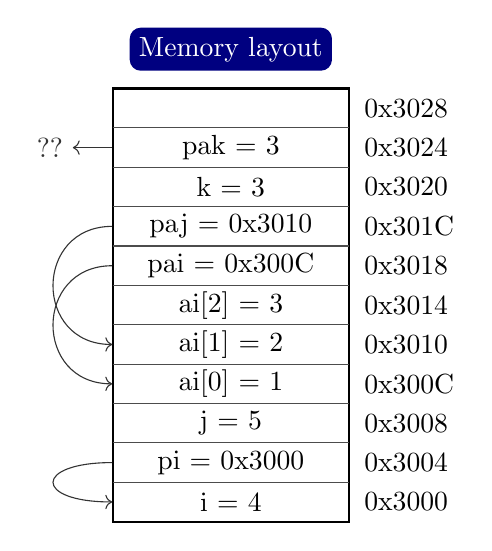
\begin{tikzpicture}
        \memorystack[size x=3cm,word size=1,block size=4,nb blocks=11]
        \onslide<2-> {\memorypush{i = 4}}
        \onslide<3-> {\memorypushpointer[pi =]{1}}
        \onslide<4-> {\memorypush{j = 5}}
        \onslide<5-> {\memorypush{ai[0] = 1}}
        \onslide<5-> {\memorypush{ai[1] = 2}}
        \onslide<5-> {\memorypush{ai[2] = 3}}
        \onslide<6-> {\memorypushpointer[pai =]{4}}
        \onslide<7-> {\memorypushpointer[paj =]{5}}
        \onslide<8-> {\memorypush{k = 3}}
        \onslide<9-> {\memorypush{pak = 3}}
        \onslide<9-> {\draw[\stackcolor!80,->] (stack10-1.west) -- +(-0.5cm,0)
          node [anchor=east] {??};}
      \end{tikzpicture}
    }
  \end{multicols}
\end{frame}

\begin{frame}[fragile]
  \frametitlecpp[11]{nullptr}
  \begin{block}{A pointer to nothing}
    \begin{itemize}
    \item if a pointer doesn't point to anything, set it to \cppinline{nullptr}
    \begin{itemize}
      \item useful to e.g.\ mark the end of a linked data structure
      \item or absence of an optional function argument (pointer)
    \end{itemize}
    \item same as setting it to 0 or \cppinline{NULL} (before \cpp11)
    \item triggers compilation error when assigned to integer
    \end{itemize}
  \end{block}
  \pause
  \begin{exampleblock}{Example code}
    \begin{cppcode*}{}
      int* ip = nullptr;
      int i = NULL;      // compiles, bug?
      int i = nullptr;   // ERROR
    \end{cppcode*}
  \end{exampleblock}
\end{frame}

\begin{frame}[fragile]
  \frametitlecpp[98]{Dynamic arrays using C}
  \begin{cppcode}
    #include <cstdlib>
    #include <cstring>

    int *bad;          // pointer to random address
    int *ai = nullptr; // better, deterministic, testable

    // allocate array of 10 ints (uninitialized)
    ai = (int*) malloc(10*sizeof(int));
    memset(ai, 0, 10*sizeof(int)); // and set them to 0

    ai = (int*) calloc(10, sizeof(int)); // both in one go

    free(ai); // release memory
  \end{cppcode}
  \begin{goodpracticeWithShortcut}{Don't use C's memory management}{C's memory management}
    Use \cppinline{std::vector} and friends or smart pointers
  \end{goodpracticeWithShortcut}
\end{frame}

\begin{frame}[fragile]
	\frametitlecpp[98]{Manual dynamic arrays using \cpp}
	\begin{cppcode}
		#include <cstdlib>
		#include <cstring>

		// allocate array of 10 ints
		int* ai = new int[10];   // uninitialized
		int* ai = new int[10]{}; // zero-initialized

		delete[] ai; // release array memory

		// allocate a single int
		int* pi = new int;
		int* pi = new int{};
		delete pi; // release scalar memory
	\end{cppcode}
	\begin{goodpracticeWithShortcut}{Don't use manual memory management}{Manual memory management}
		Use \cppinline{std::vector} and friends or smart pointers
	\end{goodpracticeWithShortcut}
\end{frame}

\subsection[NS]{Scopes / namespaces}

\begin{frame}[fragile]
  \frametitlecpp[98]{Scope}
  \begin{block}{Definition}
    Portion of the source code where a given name is valid \\
    Typically :
    \begin{itemize}
    \item simple block of code, within \cppinline{{}}
    \item function, class, namespace
    \item the global scope, i.e.\ translation unit (.cpp file + all includes)
    \end{itemize}
  \end{block}
  \begin{exampleblock}{Example}
    \begin{cppcode*}{}
      { int a;
        { int b;
        } // end of b scope
      } // end of a scope
    \end{cppcode*}
  \end{exampleblock}
\end{frame}

\begin{frame}[fragile]
  \frametitlecpp[98]{Scope and lifetime of variables}
  \begin{block}{Variable life time}
    \begin{itemize}
      \item Variables are (statically) allocated when defined
      \item Variables are freed at the end of a scope
    \end{itemize}
  \end{block}
  \begin{goodpractice}{Initialisation}
    \begin{itemize}
      \item Initialise variables when allocating them!
      \item This prevents bugs reading uninitialised memory
    \end{itemize}
  \end{goodpractice}
  \begin{multicols}{2}
    % the code has to be repeated n times here. Anyone finding a better solution
    % is welcome, but it's not a trivial task, due to the verbatim nature of minted
    \begin{overprint}[\columnwidth]
    \onslide<1>
      \begin{minted}[linenos,highlightlines=1]{cpp}
int a = 1;
{
  int b[4];
  b[0] = a;
}
// Doesn't compile here:
// b[1] = a + 1;
      \end{minted}
    \onslide<2>
      \begin{minted}[linenos,highlightlines=3]{cpp}
int a = 1;
{
  int b[4];
  b[0] = a;
}
// Doesn't compile here:
// b[1] = a + 1;
      \end{minted}
    \onslide<3>
      \begin{minted}[linenos,highlightlines=4]{cpp}
int a = 1;
{
  int b[4];
  b[0] = a;
}
// Doesn't compile here:
// b[1] = a + 1;
      \end{minted}
    \onslide<4>
      \begin{minted}[linenos,highlightlines=7]{cpp}
int a = 1;
{
  int b[4];
  b[0] = a;
}
// Doesn't compile here:
// b[1] = a + 1;
      \end{minted}
    \end{overprint}

    \columnbreak

    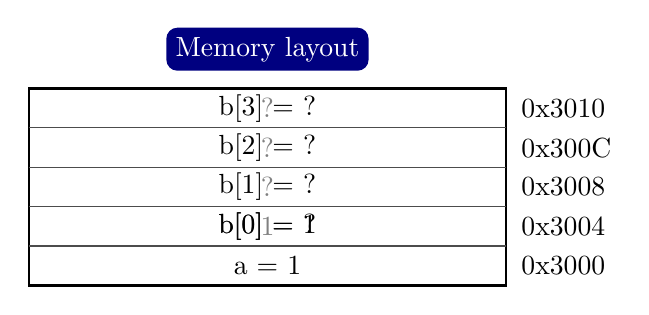
\begin{tikzpicture}
      \memorystack[word size=1, block size=4, nb blocks=5, size x = 0.5\columnwidth]
      \onslide<1-> {
        \memorypush{a = 1}
      }
      \onslide<2>{
        \memorypush{b[0] = ?}
      }
      \memorygoto{2}
      \onslide<3>{
        \memorypush{b[0] = 1}
      }
      \memorygoto{3}
      \onslide<2-3>{
        \memorypush{b[1] = ?}
        \memorypush{b[2] = ?}
        \memorypush{b[3] = ?}
      }

      \memorygoto{2}
      \onslide<4>{
        \memorypush{\color{gray} 1}
        \memorypush{\color{gray} ?}
        \memorypush{\color{gray} ?}
        \memorypush{\color{gray} ?}
        }

    \end{tikzpicture}

  \end{multicols}
\end{frame}

\begin{frame}[fragile]
  \frametitlecpp[98]{Namespaces}
  \begin{itemize}
  \item Namespaces allow to segment your code to avoid name clashes
  \item They can be embedded to create hierarchies (separator is '::')
  \end{itemize}
  \begin{multicols}{2}
    \begin{cppcode*}{gobble=2}
      int a;
      namespace n {
        int a;   // no clash
      }
      namespace p {
        int a;   // no clash
        namespace inner {
          int a; // no clash
        }
      }
      void f() {
        n::a = 3;
      }
    \end{cppcode*}
    \columnbreak
    \begin{cppcode*}{gobble=2,firstnumber=14}
      namespace p { // reopen p
        void f() {
          p::a = 6;
          a = 6;  //same as above
          ::a = 1;
          p::inner::a = 8;
          inner::a = 8;
          n::a = 3;
        }
      }
      using namespace p::inner;
      void g() {
        a = -1; // err: ambiguous
      }
  \end{cppcode*}
  \end{multicols}
\end{frame}

\begin{frame}[fragile]
  \frametitlecpp[17]{Nested namespaces}
  \begin{alertblock}{\cpp98: Old way to declare nested namespaces}
    \begin{cppcode*}{}
      namespace A {
        namespace B {
          namespace C {
            //...
          }
        }
      }
    \end{cppcode*}
  \end{alertblock}
  \begin{exampleblock}{\cpp17: Nested declaration}
    \begin{cppcode*}{}
      namespace A::B::C {
        //...
      }
    \end{cppcode*}
  \end{exampleblock}
  \begin{exampleblock}{\cpp17: Namespace alias}
    \begin{cppcode*}{}
      namespace ABC = A::B::C;
    \end{cppcode*}
  \end{exampleblock}
\end{frame}

\begin{advanced}
\begin{frame}[fragile]
  \frametitlecpp[98]{Unnamed / anonymous namespaces}
  \begin{exampleblock}{A namespace without a name!}
    \begin{cppcode*}{}
      namespace {
        int localVar;
      }
    \end{cppcode*}
  \end{exampleblock}
  \begin{block}{Purpose}
    \begin{itemize}
    \item groups a number of declarations
    \item visible only in the current translation unit
    \item but not reusable outside
    \item allows much better compiler optimizations and checking
      \begin{itemize}
      \item e.g. unused function warning
      \item context dependent optimizations
      \end{itemize}
    \end{itemize}
  \end{block}
  \begin{alertblock}{Supersedes static}
    \begin{cppcode*}{gobble=2,firstnumber=4}
      static int localVar; // equivalent C code
    \end{cppcode*}
  \end{alertblock}
\end{frame}

\begin{frame}[fragile]
  \frametitlecpp[98]{Using namespace directives}
  \begin{alertblock}{Avoid ``using namespace'' directives}
    \begin{itemize}
      \item Make all members of a namespace visible in current scope
      \item Risk of name clashes or ambiguities
    \end{itemize}
    \begin{cppcode*}{}
      using namespace std;
      cout << "We can print now\n"; // uses std::cout
    \end{cppcode*}
  \end{alertblock}
  \begin{alertblock}{Never use in headers at global scope!}
    \begin{cppcode*}{gobble=2}
      #include "PoorlyWritten.h" // using namespace std;
      struct array { ... };
      array a;  // Error: name clash with std::array
    \end{cppcode*}
  \end{alertblock}
  \begin{block}{What to do instead}
    \begin{itemize}
      \item Qualify names: \cppinline{std::vector}, \cppinline{std::cout}, \ldots
      \item Put things that belong together in the same namespace
      \item Use \textit{using declarations} in local scopes: \cppinline{using std::cout;}
    \end{itemize}
  \end{block}
\end{frame}

\end{advanced}

\subsection[Class/Enum]{Class and enum types}

\begin{frame}[fragile]
  \frametitlecpp[98]{struct}
  \begin{mdframed}[style=simplebox]
    \center ``members'' grouped together under one name
  \end{mdframed}
  \begin{multicols}{2}
    \begin{cppcode*}{}
      struct Individual {
        unsigned char age;
        float weight;
      };

      Individual student;
      student.age = 25;
      student.weight = 78.5f;

      Individual teacher = {
        45, 67.0f
      };
    \end{cppcode*}
    \columnbreak
    \begin{cppcode*}{firstnumber=14}
      Individual *ptr = &student;
      ptr->age = 25;
      // same as: (*ptr).age = 25;
    \end{cppcode*}
    \pause
    \vfill
    \hspace{-1.5cm}
    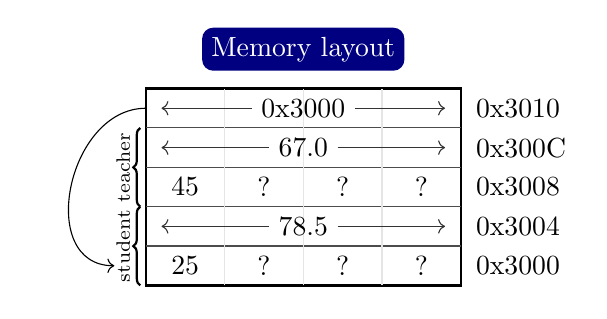
\begin{tikzpicture}
      \memorystack[nb blocks=5]
      \onslide<3-> {
        \memorypush{25,?,?,?}
        \memorypushwidevalue{78.5}
        \memorystruct{1}{2}{\scriptsize student}
      }
      \onslide<4-> {
        \memorypush{45,?,?,?}
        \memorypushwidevalue{67.0}
        \memorystruct{3}{4}{\scriptsize teacher}
      }
      \onslide<5-> {
        \memorypushwidevalue{0x3000}
        \draw[->] (0,2.25) .. controls +(left:1) and +(left:1) .. (-.4,.25);
      }
    \end{tikzpicture}
    \vfill \null
  \end{multicols}
\end{frame}

\begin{frame}[fragile]
  \frametitlecpp[98]{union}
  \begin{mdframed}[style=simplebox]
    \center ``members'' packed together at same memory location
  \end{mdframed}
  \begin{multicols}{2}
    \begin{cppcode*}{}
      union Duration {
        int seconds;
        short hours;
        char days;
      };
      Duration d1, d2, d3;
      d1.seconds = 259200;
      d2.hours = 72;
      d3.days = 3;
      d1.days = 3; // d1.seconds overwritten
      int a = d1.seconds; // d1.seconds is garbage
    \end{cppcode*}
    \pause
    \columnbreak
    \null \vfill
    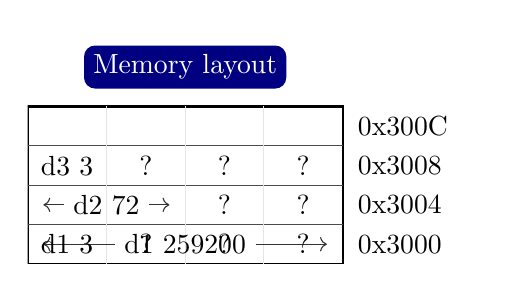
\begin{tikzpicture}
      \clip (0,0) rectangle (6cm, 3cm);
      \memorystack[word size=4,nb blocks=4]
      \visible<3-5>{\memorypushwidevalue{d1 259200}}
      \onslide<4->{\memorypushhalfvalue{d2 72}}
      \memorygoto{2}
      \onslide<4->{\memorypush{,,?,?}}
      \onslide<5->{\memorypush{d3 3,?,?,?}}
      \memorygoto{1}
      \onslide<6->{\memorypush{d1 3,?,?,?}}
    \end{tikzpicture}
    \vfill \null
  \end{multicols}
  \onslide<7->{
  \begin{goodpractice}{Avoid unions}
    \begin{itemize}
      \item Starting with \cpp17: prefer \cppinline{std::variant}
    \end{itemize}
  \end{goodpractice}
  }
\end{frame}

\begin{frame}[fragile]
  \frametitlecpp[98]{Enums}
  \begin{block}{}
    \begin{itemize}
        \item use to declare a list of related constants (enumerators)
        \item has an underlying integral type
        \item enumerator names leak into enclosing scope
    \end{itemize}
  \end{block}
  \begin{multicols}{2}
    \begin{cppcode*}{}
      enum VehicleType {

        BIKE,  // 0
        CAR,   // 1
        BUS,   // 2
      };
      VehicleType t = CAR;
    \end{cppcode*}
    \columnbreak
    \begin{cppcode*}{firstnumber=8}
      enum VehicleType
        : int { // C++11
        BIKE = 3,
        CAR = 5,
        BUS = 7,
      };
      VehicleType t2 = BUS;
    \end{cppcode*}
  \end{multicols}
\end{frame}

\begin{frame}[fragile]
  \frametitlecpp[11]{Scoped enumeration, aka enum class}
  \begin{block}{Same syntax as enum, with scope}
    \begin{cppcode*}{}
      enum class VehicleType { Bus, Car };
      VehicleType t = VehicleType::Car;
    \end{cppcode*}
  \end{block}
  \pause
  \begin{exampleblock}{Only advantages}
    \begin{itemize}
    \item scopes enumerator names, avoids name clashes
    \item strong typing, no automatic conversion to int
    \end{itemize}
    \small
    \begin{cppcode*}{firstnumber=3}
      enum VType { Bus, Car }; enum Color { Red, Blue };
      VType t = Bus;
      if (t == Red) { /* We do enter */ }
      int a = 5 * Car; // Ok, a = 5

      enum class VT { Bus, Car }; enum class Col { Red, Blue };
      VT t = VT::Bus;
      if (t == Col::Red) { /* Compiler error */ }
      int a = t * 5;       // Compiler error
    \end{cppcode*}
  \end{exampleblock}
\end{frame}

\begin{frame}[fragile]
  \frametitlecpp[98]{More sensible example}
  \begin{multicols}{2}
    \begin{cppcode*}{}
      enum class ShapeType {
        Circle,
        Rectangle
      };

      struct Rectangle {
        float width;
        float height;
      };
    \end{cppcode*}
    \columnbreak
    \pause
    \begin{cppcode*}{firstnumber=10}
      struct Shape {
        ShapeType type;
        union {
          float radius;
          Rectangle rect;
        };
      };
    \end{cppcode*}
  \end{multicols}
  \pause
  \begin{multicols}{2}
    \begin{cppcode*}{firstnumber=17}
      Shape s;
      s.type =
        ShapeType::Circle;
      s.radius = 3.4;

    \end{cppcode*}
    \columnbreak
    \begin{cppcode*}{firstnumber=20}
      Shape t;
      t.type =
        Shapetype::Rectangle;
      t.rect.width = 3;
      t.rect.height = 4;
    \end{cppcode*}
  \end{multicols}
\end{frame}

\begin{frame}[fragile]
  \frametitle{typedef and using \hfill \cpp98 / \cpp11}
  Used to create type aliases
  \begin{alertblock}{\cpp98}
    \begin{cppcode*}{}
      typedef std::uint64_t myint;
      myint count = 17;
      typedef float position[3];
    \end{cppcode*}
  \end{alertblock}
  \begin{exampleblock}{\cpp11}
    \begin{cppcode*}{firstnumber=4}
      using myint = std::uint64_t;
      myint count = 17;
      using position = float[3];

      template <typename T> using myvec = std::vector<T>;
      myvec<int> myintvec;
    \end{cppcode*}
  \end{exampleblock}
\end{frame}

\subsection[Refs]{References}

\begin{frame}[fragile]
  \frametitlecpp[98]{References}
  \begin{block}{References}
    \begin{itemize}
      \item References allow for direct access to another object
      \item They can be used as shortcuts / better readability
      \item They can be declared \mintinline{cpp}{const} to allow only read access
      \item They can be used as function arguments
    \end{itemize}
  \end{block}

  \begin{exampleblock}{Example:}
    \begin{cppcode*}{gobble=2}
      int i = 2;
      int &iref = i; // access to i
      iref = 3;      // i is now 3

      // const reference to a member:
      struct A { int x; int y; } a;
      const int &x = a.x; // direct read access to A's x
      x = 4;              // doesn't compile
    \end{cppcode*}
  \end{exampleblock}
\end{frame}

\begin{frame}[fragile]
  \frametitlecpp[98]{Pointers vs References}
  \begin{block}{Specificities of reference}
    \begin{itemize}
    \item natural syntax
    \item must be assigned when defined, cannot be \mintinline{cpp}{nullptr}
    \item cannot be reassigned
    \item non-const references to temporary objects are not allowed
    \end{itemize}
  \end{block}
  \begin{block}{Advantages of pointers}
    \begin{itemize}
    \item can be reassigned to point elsewhere or to \mintinline{cpp}{nullptr}
    \item clearly indicates that argument may be modified
    \end{itemize}
  \end{block}
  \pause
  \begin{goodpractice}{References}
    \begin{itemize}
      \item Always use references when you can
      \item Consider that a reference will be modified
      \item Use constness when it's not the case
    \end{itemize}
  \end{goodpractice}
\end{frame}

\subsection[$f()$]{Functions}

\begin{frame}[fragile]
  \frametitlecpp[98]{Functions}
  \begin{multicols}{2}
    \begin{cppcode*}{gobble=2}
      // with return type
      int square(int a) {
        return a * a;
      }

      // multiple parameters
      int mult(int a,
               int b) {
        return a * b;
      }
    \end{cppcode*}
    \columnbreak
    \begin{cppcode*}{gobble=2,firstnumber=11}
      // no return
      void log(char* msg) {
        std::cout << msg;
      }

      // no parameter
      void hello() {
        std::cout << "Hello World";
      }
    \end{cppcode*}
  \end{multicols}
\end{frame}

\begin{frame}[fragile]
  \frametitlecpp[98]{Function default arguments}
  \begin{multicols}{2}
    \begin{cppcode*}{gobble=2}
      // must be the trailing
      // argument
      int add(int a,
              int b = 2) {
        return a + b;
      }
      // add(1) == 3
      // add(3,4) == 7

    \end{cppcode*}
    \columnbreak
    \begin{cppcode*}{gobble=2,firstnumber=11}
      // multiple default
      // arguments are possible
      int add(int a = 2,
              int b = 2) {
        return a + b;
      }
      // add() == 4
      // add(3) == 5
    \end{cppcode*}
  \end{multicols}
\end{frame}


\Scontents*[store-cmd=code_bigStruct]{
struct BigStruct {...};
BigStruct s;

// parameter by value
void printVal(BigStruct p) {
  ...
}
printVal(s); // copy

// parameter by reference
void printRef(BigStruct &q) {
  ...
}
printRef(s); // no copy
}
\begin{frame}[fragile]
  \frametitlecpp[98]{Functions: parameters are passed by value}
  \begin{multicols}{2}
    \begin{overprint}[\columnwidth]
      \onslide<1-2>
      \highlightCppCode{2}{code_bigStruct}
      \onslide<3>
      \highlightCppCode{5,8}{code_bigStruct}
      \onslide<4->
      \highlightCppCode{11,14}{code_bigStruct}
    \end{overprint}
    \columnbreak
    \null \vfill
    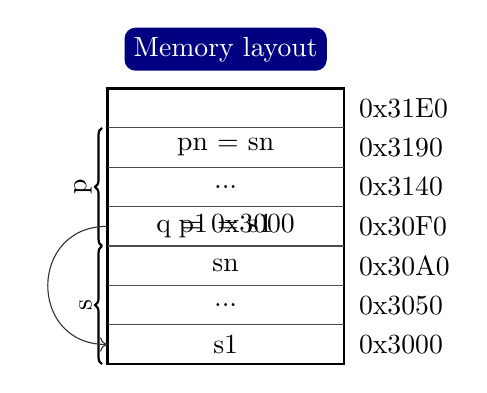
\begin{tikzpicture}
      \memorystack[word size=1, block size=80, nb blocks=7, size x=3cm]
      \onslide<2-> {
        \memorypush{s1}
        \memorypush{...}
        \memorypush{sn}
        \memorystruct{1}{3}{s}
      }
      \onslide<3> {
        \memorypush{p1 = s1}
        \memorypush{...}
        \memorypush{pn = sn}
        \memorystruct{4}{6}{p}
      }
      \memorygoto{4}
      \onslide<4> {
        \memorypushpointer[q =]{1}
      }
    \end{tikzpicture}
    \vfill \null
  \end{multicols}
\end{frame}

\Scontents*[store-cmd=code_smallStruct]{
struct SmallStruct {int a;};
SmallStruct s = {1};

void changeVal(SmallStruct p) {
  p.a = 2;
}
changeVal(s);
// s.a == 1

void changeRef(SmallStruct &q) {
  q.a = 2;
}
changeRef(s);
// s.a == 2
}
\begin{frame}[fragile]
  \frametitlecpp[98]{Functions: pass by value or reference?}
  \begin{multicols}{2}
    \begin{overprint}[\columnwidth]
      \onslide<1>
      \highlightCppCode{}{code_smallStruct}
      \onslide<2>
      \highlightCppCode{2}{code_smallStruct}
      \onslide<3>
      \highlightCppCode{4,7}{code_smallStruct}
      \onslide<4>
      \highlightCppCode{5}{code_smallStruct}
      \onslide<5>
      \highlightCppCode{8}{code_smallStruct}
      \onslide<6>
      \highlightCppCode{10,13}{code_smallStruct}
      \onslide<7>
      \highlightCppCode{11}{code_smallStruct}
      \onslide<8>
      \highlightCppCode{14}{code_smallStruct}
    \end{overprint}
    \columnbreak
    \null \vfill
    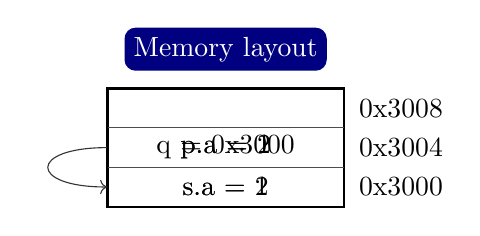
\begin{tikzpicture}
      \memorystack[word size=1, block size=4, nb blocks=3, size x=3cm]
      \onslide<2-6> {
        \memorypush{s.a = 1}
      }
      \memorygoto{1}
      \onslide<7-> {
        \memorypush{s.a = 2}
      }

      \memorygoto{2}
      \onslide<3> {
        \memorypush{p.a = 1}
      }
      \memorygoto{2}
      \onslide<4> {
        \memorypush{p.a = 2}
      }
      \memorygoto{2}
      \onslide<6-7> {
        \memorypushpointer[q =]{1}
      }
      \end{tikzpicture}
    \vfill \null
  \end{multicols}
\end{frame}

\begin{frame}[fragile]
  \frametitlecpp[98]{Pass by value, reference or pointer}
  \begin{block}{Different ways to pass arguments to a function}
    \begin{itemize}
    \item By default, arguments are passed by value (= copy) \\
          good for small types, e.g.\ numbers
    \item Use references for parameters to avoid copies \\
          good for large types, e.g.\ objects
    \item Use \cppinline{const} for safety and readability whenever possible
    \end{itemize}
  \end{block}
  \pause
  \begin{block}{Syntax}
    \begin{cppcode*}{escapeinside=||}
struct T {...}; T a;
void fVal(T value);        fVal(a);   // by value
void fRef(const T &value); fRef(a);   // by reference
void fPtr(const T *value); fPtr(|{\setlength{\fboxsep}{0pt}\color{gray}\colorbox{yellow}{\textsc{&}}}|a);  // by pointer
void fWrite(T &value);     fWrite(a); // non-const ref
    \end{cppcode*}
  \end{block}
\end{frame}

\begin{frame}[fragile]
    \frametitlecpp[98]{Overloading}
    \begin{block}{Overloading}
        \begin{itemize}
            \item We can have multiple functions with the same name
            \item They must have different parameter lists
            \item A different return type alone is not allowed
            \item Default arguments can cause ambiguities
            \item All functions with the same name form an ``overload set''
        \end{itemize}
    \end{block}
    \begin{exampleblock}{}
        \begin{cppcode*}{gobble=6}
            int sum(int b);             // 1
            int sum(int b, int c);      // 2, ok, overload
            // float sum(int b, int c); // disallowed
            sum(42); // calls 1
            sum(42, 43); // calls 2
            int sum(int b, int c, int d = 4); // 3, overload
            sum(42, 43, 44); // calls 3
            sum(42, 43);     // error: ambiguous, 2 or 3
        \end{cppcode*}
    \end{exampleblock}
\end{frame}

\begin{frame}[fragile]
  \frametitlecpp[98]{Functions}
  \begin{exercise}{Functions}
    Familiarise yourself with pass by value / pass by reference.
    \begin{itemize}
      \item Go to \texttt{code/functions}
      \item Look at \texttt{functions.cpp}
      \item Compile it (\texttt{make}) and run the program (\texttt{./functions})
      \item Work on the tasks that you find in \texttt{functions.cpp}
    \end{itemize}
  \end{exercise}
\end{frame}

\begin{frame}[fragile]
  \frametitlecpp[98]{Functions: good practices}
  \begin{onlyenv}<1>
    \begin{goodpractice}{Write readable functions}
      \begin{itemize}
        \item Keep functions short
        \item Do one logical thing (single-responsibility principle)
        \item Use expressive names
        \item Document non-trivial functions
      \end{itemize}
    \end{goodpractice}
    \begin{exampleblock}{Example: Good}
      \begin{cppcode*}{gobble=2}
        /// Count number of dilepton events in data.
        /// \param d Dataset to search.
        unsigned int countDileptons(Data d) {
          selectEventsWithMuons(d);
          selectEventsWithElectrons(d);
          return d.size();
        }
      \end{cppcode*}
    \end{exampleblock}
  \end{onlyenv}
  \begin{onlyenv}<2->
    \begin{alertblock}{Example: don't! Everything in one long function}
      \begin{multicols}{2}
        \begin{cppcode*}{gobble=6}
          unsigned int runJob() {
            // Step 1: data
            Data data;
            data.resize(123456);
            data.fill(...);

            // Step 2: muons
            for (....) {
              if (...) {
                data.erase(...);
              }
            }
            // Step 3: electrons
            for (....) {
        \end{cppcode*}
        \columnbreak
        \begin{cppcode*}{gobble=6,firstnumber=last}
              if (...) {
                data.erase(...);
              }
            }

            // Step 4: dileptons
            int counter = 0;
            for (....) {
              if (...) {
                counter++;
              }
            }

            return counter;
          }
        \end{cppcode*}
      \end{multicols}
    \end{alertblock}
  \end{onlyenv}
\end{frame}

\subsection[Op]{Operators}

\begin{frame}[fragile]
  \frametitlecpp[98]{Operators(1)}
  \begin{block}{Binary and Assignment Operators}
    \begin{cppcode*}{}
      int i = 1 + 4 - 2;  // 3
      i *= 3;             // 9, short for: i = i * 3;
      i /= 2;             // 4
      i = 23 % i;         // modulo => 3
    \end{cppcode*}
  \end{block}
  \pause
  \begin{block}{Increment / Decrement Operators \uncover<3->{\hfill \alert{\bf Use wisely}}}
    \begin{cppcode*}{}
      int i = 0; i++; // i = 1
      int j = ++i;    // i = 2, j = 2
      int k = i++;    // i = 3, k = 2
      int l = --i;    // i = 2, l = 2
      int m = i--;    // i = 1, m = 2
    \end{cppcode*}
  \end{block}
\end{frame}

\begin{frame}[fragile]
  \frametitlecpp[98]{Operators(2)}
  \begin{block}{Bitwise and Assignment Operators}
    \begin{cppcode*}{}
      unsigned i = 0xee & 0x55;  // 0x44
      i |= 0xee;                 // 0xee
      i ^= 0x55;                 // 0xbb
      unsigned j = ~0xee;        // 0xffffff11
      unsigned k = 0x1f << 3;    // 0xf8
      unsigned l = 0x1f >> 2;    // 0x7
    \end{cppcode*}
  \end{block}
  \pause
  \begin{block}{Logical Operators}
    \begin{cppcode*}{}
      bool a = true;
      bool b = false;
      bool c = a && b;    // false
      bool d = a || b;    // true
      bool e = !d;        // false
    \end{cppcode*}
  \end{block}
\end{frame}

\begin{frame}[fragile]
  \frametitlecpp[98]{Operators(3)}
  \begin{block}{Comparison Operators}
    \begin{cppcode*}{}
      bool a = (3 == 3);  // true
      bool b = (3 != 3);  // false
      bool c = (4 <  4);  // false
      bool d = (4 <= 4);  // true
      bool e = (4 >  4);  // false
      bool f = (4 >= 4);  // true
    \end{cppcode*}
  \end{block}
  \pause
  \begin{block}{Precedences \uncover<3->{\hfill \alert{\bf Avoid}\uncover<4->{\color{green} \bf\ - use parentheses}}}
    \begin{cppcode*}{linenos=false}
      c &= 1+(++b)|(a--)*4%5^7; // ???
    \end{cppcode*}
    Details can be found on {\color{blue!50!white} \href{https://en.cppreference.com/w/cpp/language/operator_precedence}{cppreference}}
  \end{block}
\end{frame}

\subsection[Control]{Control structures}

\begin{frame}[fragile]
  \frametitlecpp[98]{Control structures: if}
  \begin{block}{if syntax}
    \begin{cppcode*}{}
      if (condition1) {
        Statement1; Statement2;
      } else if (condition2)
        OnlyOneStatement;
      else {
        Statement3;
        Statement4;
      }
    \end{cppcode*}
    \begin{itemize}
      \item The \cppinline{else} and \cppinline{else if} clauses are optional
      \item The \cppinline{else if} clause can be repeated
      \item Braces are optional if there is a single statement
    \end{itemize}
  \end{block}
\end{frame}

\begin{frame}[fragile]
  \frametitlecpp[98]{Control structures: if}
  \begin{exampleblock}{Practical example}
    \begin{cppcode*}{}
      int collatz(int a) {
        if (a <= 0) {
          std::cout << "not supported\n";
          return 0;
        } else if (a == 1) {
          return 1;
        } else if (a%2 == 0) {
          return collatz(a/2);
        } else {
          return collatz(3*a+1);
        }
      }
    \end{cppcode*}
  \end{exampleblock}
\end{frame}

\begin{frame}[fragile]
  \frametitlecpp[98]{Control structures: conditional operator}
  \begin{block}{Syntax}
    \begin{cppcode*}{linenos=false}
      test ? expression1 : expression2;
    \end{cppcode*}
    \vspace{-0.2cm}
    \begin{itemize}
      \item If test is \cppinline{true} \cppinline{expression1} is returned
      \item Else, \cppinline{expression2} is returned
    \end{itemize}
  \end{block}
  \pause
  \begin{exampleblock}{Practical example}
    \begin{cppcode*}{}
      int collatz(int a) {
        return a==1 ? 1 : collatz(a%2==0 ? a/2 : 3*a+1);
      }
    \end{cppcode*}
  \end{exampleblock}
  \pause
  \begin{alertblock}{Do not abuse it}
    \begin{itemize}
      \item Explicit \cppinline{if}s are generally easier to read
      \item Use the ternary operator with short conditions and expressions
      \item Avoid nesting
    \end{itemize}
  \end{alertblock}
\end{frame}

\begin{frame}[fragile]
  \frametitlecpp[98]{Control structures: switch}
  \begin{block}{Syntax}
    \begin{cppcode*}{gobble=0}
      switch(identifier) {
        case c1 : statements1; break;
        case c2 : statements2; break;
        case c3 : statements3; break;
        ...
        default : instructiond; break;
      }
    \end{cppcode*}
    \begin{itemize}
      \item The \cppinline{break} statement is not mandatory but...
      \item Cases are entry points, not independent pieces
      \item Execution falls through to the next case without a \cppinline{break}!
      \item The \cppinline{default} case may be omitted
    \end{itemize}
  \end{block}
  \pause
  \begin{alertblock}{Use break}
    Avoid \cppinline{switch} statements with fall-through cases
  \end{alertblock}
\end{frame}

\begin{frame}[fragile]
  \frametitlecpp[98]{Control structures: switch}
  \begin{exampleblock}{Practical example}
    \begin{cppcode*}{}
      enum class Lang { French, German, English, Other };
      ...
      switch (language) {
      case Lang::French:
        std::cout << "Bonjour";
        break;
       case Lang::German:
        std::cout << "Guten Tag";
        break;
      case Lang::English:
        std::cout << "Good morning";
        break;
      default:
        std::cout << "I do not speak your language";
      }
    \end{cppcode*}
  \end{exampleblock}
\end{frame}

\AtBeginEnvironment{minted}{\renewcommand{\fcolorbox}[4][]{#4}}

\begin{frame}[fragile]
  \frametitlecpp[17]{\texttt{[[fallthrough]]} attribute}
  \begin{block}{New compiler warning}
    Since \cpp17, compilers are encouraged to warn on fall-through
  \end{block}
  \begin{exampleblock}{\cpp17}
    \begin{cppcode*}{}
      switch (c) {
        case 'a':
          f();    // Warning emitted
        case 'b': // Warning emitted
        case 'c':
          g();
          [[fallthrough]]; // Warning suppressed
        case 'd':
          h();
      }
    \end{cppcode*}
  \end{exampleblock}
\end{frame}

\begin{frame}[fragile]
  \frametitlecpp[17]{Init-statements for if and switch}
  \begin{block}{}
    Allows to limit variable scope in \cppinline{if} and \cppinline{switch} statements
  \end{block}
  \begin{exampleblock}{\cpp17}
    \begin{cppcode*}{}
      if (Value val = GetValue(); condition(val)) {
        f(val);
      } else {
        g(val);
      }
      h(val); // compile error
    \end{cppcode*}
  \end{exampleblock}
  \pause
  \begin{alertblock}{\cpp98}
    Don't confuse with a variable declaration as condition:
    \begin{cppcode*}{firstnumber=7}
      if (Value* val = GetValuePtr())
        f(*val);
    \end{cppcode*}
  \end{alertblock}
\end{frame}

\begin{frame}[fragile]
  \frametitlecpp[98]{Control structures: for loop}
  \begin{block}{for loop syntax}
    \begin{cppcode*}{}
      for(initializations; condition; increments) {
        statements;
      }
    \end{cppcode*}
    \vspace{-0.2cm}
    \begin{itemize}
      \item Initializations and increments are comma separated
      \item Initializations can contain declarations
      \item Braces are optional if loop body is a single statement
    \end{itemize}
  \end{block}
  \pause
  \begin{exampleblock}{Practical example}
    \begin{cppcode*}{firstnumber=4}
      for(int i = 0, j = 0 ; i < 10 ; i++, j = i*i) {
        std::cout << i << "^2 is " << j << '\n';
      }
    \end{cppcode*}
  \end{exampleblock}
  \pause
  \begin{goodpracticeWithShortcut}{Don't abuse the \texttt{for} syntax}{\texttt{for} syntax}
    \begin{itemize}
      \item The \cppinline{for} loop head should fit in 1-3 lines
    \end{itemize}
  \end{goodpracticeWithShortcut}
\end{frame}

\begin{frame}[fragile]
  \frametitlecpp[11]{Range-based loops}
  \begin{block}{Reason of being}
    \begin{itemize}
    \item Simplifies loops over ``ranges'' tremendously
    \item Especially with STL containers and ranges
    \end{itemize}
  \end{block}
  \begin{block}{Syntax}
    \begin{cppcode*}{}
      for ( type iteration_variable : range ) {
        // body using iteration_variable
      }
    \end{cppcode*}
  \end{block}
  \begin{exampleblock}{Example code}
    \begin{cppcode*}{firstnumber=4}
      int v[4] = {1,2,3,4};
      int sum = 0;
      for (int a : v) { sum += a; }
    \end{cppcode*}
  \end{exampleblock}
\end{frame}

\begin{frame}[fragile]
  \frametitlecpp[20]{Init-statements for range-based loops}
  \begin{block}{}
    Allows to limit variable scope in range-based loops
  \end{block}
  \begin{alertblock}{\cpp17}
    \begin{cppcode*}{}
      std::array data = {"hello", ",", "world"};
      std::size_t i = 0;
      for (auto& d : data) {
        std::cout << i++ << ' ' << d << '\n';
      }
    \end{cppcode*}
  \end{alertblock}
  \begin{exampleblock}{\cpp20}
    \begin{cppcode*}{firstnumber=6}
      for (std::size_t i = 0; auto& d : data) {
        std::cout << i++ << ' ' << d << '\n';
      }
    \end{cppcode*}
  \end{exampleblock}
\end{frame}

\begin{frame}[fragile]
  \frametitlecpp[98]{Control structures: while loop}
  \begin{block}{while loop syntax}
    \begin{cppcode*}{}
      while(condition) {
        statements;
      }
      do {
        statements;
      } while(condition);
    \end{cppcode*}
    \begin{itemize}
      \item Braces are optional if the body is a single statement
    \end{itemize}
  \end{block}
  \pause
  \begin{alertblock}{Bad example}
    \begin{cppcode*}{}
      while (n != 1)
        if (0 == n%2) n /= 2;
        else n = 3 * n + 1;
    \end{cppcode*}
  \end{alertblock}
\end{frame}

\begin{frame}[fragile]
  \frametitlecpp[98]{Control structures: jump statements}
  \begin{block}{}
    \begin{description}
    \item[break] Exits the loop and continues after it
    \item[continue] Goes immediately to next loop iteration
    \item[return] Exits the current function
    \item[goto] Can jump anywhere inside a function, avoid!
    \end{description}
  \end{block}
  \pause
  \begin{alertblock}{Bad example}
    \begin{cppcode*}{}
      while (1) {
        if (n == 1) break;
        if (0 == n%2) {
          std::cout << n << '\n';
          n /= 2;
          continue;
        }
        n = 3 * n + 1;
      }
    \end{cppcode*}
  \end{alertblock}
\end{frame}

\begin{frame}[fragile]
  \frametitlecpp[11]{Control structures}
  \begin{exerciseWithShortcut}{Control structures}{Control structs}
    Familiarise yourself with different kinds of control structures. Re-implement them in different ways.
    \begin{itemize}
      \item Go to \texttt{code/control}
      \item Look at \texttt{control.cpp}
      \item Compile it (\texttt{make}) and run the program (\texttt{./control})
      \item Work on the tasks that you find in \texttt{README.md}
    \end{itemize}
  \end{exerciseWithShortcut}
\end{frame}

\subsection[.h]{Headers and interfaces}

\begin{frame}[fragile]
  \frametitlecpp[98]{Headers and interfaces}
  \begin{block}{Interface}
    Set of declarations defining some functionality
    \begin{itemize}
    \item Put in a so-called ``header file''
    \item The implementation exists somewhere else
    \end{itemize}
  \end{block}
  \begin{block}{Header: hello.hpp}
    \begin{cppcode*}{linenos=false}
      void printHello();
    \end{cppcode*}
  \end{block}
  \begin{block}{Usage: myfile.cpp}
    \begin{cppcode*}{}
      #include "hello.hpp"
      int main() {
        printHello();
      }
    \end{cppcode*}
  \end{block}
\end{frame}

\begin{frame}[fragile]
  \frametitlecpp[98]{Preprocessor}
  \begin{cppcode}
    // file inclusion
    #include "hello.hpp"
    // macro constants and function-style macros
    #define MY_GOLDEN_NUMBER 1746
    #define CHECK_GOLDEN(x) if ((x) != MY_GOLDEN_NUMBER) \
      std::cerr << #x " was not the golden number\n";
    // compile time or platform specific configuration
    #if defined(USE64BITS) || defined(__GNUG__)
      using myint = std::uint64_t;
    #elif
      using myint = std::uint32_t;
    #endif
  \end{cppcode}
  \pause
  \begin{goodpractice}[preprocessor]{Use preprocessor only in very restricted cases}
    \begin{itemize}
      \item Conditional inclusion of headers
      \item Customization for specific compilers/platforms
    \end{itemize}
  \end{goodpractice}
\end{frame}

\begin{frame}[fragile]
  \frametitlecpp[98]{Header include guards}
  \begin{block}{Problem: redefinition by accident}
    \begin{itemize}
      \item Headers may define new names (e.g.\ types)
      \item Multiple (transitive) inclusions of a header would define those names multiple times, which is a compile error
      \item Solution: guard the content of your headers!
    \end{itemize}
  \end{block}
  \begin{block}{Include guards}
    \begin{cppcode*}{}
      #ifndef MY_HEADER_INCLUDED
      #define MY_HEADER_INCLUDED
      ... // header file content
      #endif
    \end{cppcode*}
  \end{block}
  \begin{block}{Pragma once (non-standard)}
    \begin{cppcode*}{}
      #pragma once
      ... // header file content
    \end{cppcode*}
  \end{block}
\end{frame}

\begin{frame}[fragile]
  \frametitlecpp[98]{Header / source separation}
  \begin{goodpractice}[Header / source]{Headers and source files}
    \begin{itemize}
      \item Headers should contain declarations of functions / classes
        \begin{itemize}
          \item Only create them if interface is used somewhere else
        \end{itemize}
      \item Might be included/compiled many times
      \item Good to keep them short
      \item Minimise \cppinline{#include} statements
      \item Put long code in implementation files. Exceptions:
        \begin{itemize}
          \item Short functions
          \item Templates and constexpr functions
        \end{itemize}
    \end{itemize}
  \end{goodpractice}
\end{frame}

\subsection[auto]{Auto keyword}

\begin{frame}[fragile]
  \frametitlecpp[11]{Auto keyword}
  \begin{block}{Reason of being}
    \begin{itemize}
    \item Many type declarations are redundant
    \item They are often a source for compiler warnings and errors
    \item Using auto prevents unwanted/unnecessary type conversions
    \end{itemize}
    \begin{cppcode*}{}
      std::vector<int> v;
      float a = v[3];    // conversion intended?
      int b = v.size();  // bug? unsigned to signed
    \end{cppcode*}
  \end{block}
  \pause
  \begin{block}{Practical usage}
    \begin{cppcode*}{}
      std::vector<int> v;
      auto a = v[3];
      const auto b = v.size(); // std::size_t
      int sum{0};
      for (auto n : v) { sum += n; }
    \end{cppcode*}
  \end{block}
\end{frame}

\begin{frame}[fragile]
  \frametitlecpp[98]{Loops, references, auto}
  \begin{exerciseWithShortcut}{Loops, references, auto}{Loops, refs, auto}
    Familiarise yourself with range-based for loops and references
    \begin{itemize}
      \item Go to \texttt{exercises/loopsRefsAuto}
      \item Look at \texttt{loopsRefsAuto.cpp}
      \item Compile it (\texttt{make}) and run the program (\texttt{./loopsRefsAuto})
      \item Work on the tasks that you find in \texttt{loopsRefsAuto.cpp}
    \end{itemize}
  \end{exerciseWithShortcut}
\end{frame}

\begin{advanced}
  \subsection[inline]{Inline keyword}

\begin{frame}[fragile]
  \frametitlecpp[98]{Inline keyword}
  \begin{block}{Inline functions originally}
    \begin{itemize}
      \item Applies to a function to tell the compiler to inline it
        \begin{itemize}
        \item That is, replace function calls by the function's content\\
              (similar to how a macro works)
        \end{itemize}
      \item Only a hint, compiler can still choose to not inline
      \item Avoids call overhead at the cost of increasing binary size
    \end{itemize}
  \end{block}
  \begin{exampleblock}{Major side effect}
    \begin{itemize}
      \item The linker reduces the duplicated functions into one
      \item An inline function definition can thus live in header files
    \end{itemize}
  \end{exampleblock}
  \begin{block}{}
    \begin{cppcode*}{}
      inline int mult(int a, int b) {
        return a * b;
      }
    \end{cppcode*}
  \end{block}
\end{frame}

\begin{frame}[fragile]
  \frametitlecpp[98]{Inline keyword}
  \begin{block}{Inline functions nowadays}
    \begin{itemize}
      \item Compilers can judge far better when to inline or not
        \begin{itemize}
        \item thus primary purpose is gone
        \end{itemize}
      \item Putting functions into headers became main purpose
      \item Many types of functions are marked \mintinline{cpp}{inline} by default:
      \begin{itemize}
        \item function templates
        \item \mintinline{cpp}{constexpr} functions
        \item class member functions
      \end{itemize}
    \end{itemize}
  \end{block}
\end{frame}

\begin{frame}[fragile]
  \frametitlecpp[17]{Inline keyword}
  \begin{block}{Inline variables}
    \begin{itemize}
      \item Global (or \mintinline{cpp}{static} member) variable specified as \mintinline{cpp}{inline}
      \item Same side effect, linker merges all occurrences into one
      \item Allows to define global variables/constants in headers
    \end{itemize}
  \end{block}
  \begin{block}{}
    \small
    \begin{cppcode*}{}
      // global.h
      inline int count = 0;
      inline const std::string filename = "output.txt";
      // a.cpp
      #include "global.h"
      int f() { return count; }
      // b.cpp
      #include "global.h"
      void g(int i) { count += i; }
    \end{cppcode*}
  \end{block}
  \begin{alertblock}{}
    \begin{itemize}
      \item Avoid global variables! Global constants are fine.
    \end{itemize}
  \end{alertblock}
\end{frame}

  \subsection[assert]{Assertions}

\begin{frame}[fragile]
  \frametitlecpp[98]{Assertions}
  \begin{block}{Checking invariants in a program}
    \begin{itemize}
      \item An invariant is a property that is guaranteed to be true during certain phases of a program, and the program might crash or yield wrong results if it is violated
      \begin{itemize}
        \item ``Here, `a' should always be positive''
      \end{itemize}
      \item This can be checked using \mintinline{cpp}{assert}
      \item The program will be aborted if the assertion fails
    \end{itemize}
  \end{block}
  \begin{exampleblockGB}{\texttt{assert} in practice}{https://godbolt.org/z/eo78cY7hM}{\texttt{assert}}
    \begin{overprint}
    \onslide<1>
    \begin{cppcode*}{}
      #include <cassert>
      double f(double a) {
        // [...] do stuff with a
        // [...] that should leave it positive
        assert(a > 0.);
        return std::sqrt(a);
      }
    \end{cppcode*}
    \onslide<2>
    \begin{Verbatim}
% ./testAssert
Assertion failed: (a > 0.), function f,
                  file testAssert.cpp, line 5.
Abort trap: 6
    \end{Verbatim}
    \end{overprint}
  \end{exampleblockGB}
\end{frame}

\begin{frame}[fragile]
  \frametitlecpp[98]{Assertions}
  \begin{goodpractice}{Assert}
    \begin{itemize}
      \item Assertions are mostly for developers and debugging
      \item Use them to check important invariants of your program
      \item Prefer handling user-facing errors with helpful error messages/exceptions
      \item Assertions can impact the speed of a program
      \begin{itemize}
        \item Assertions are disabled when the macro \mintinline{cpp}{NDEBUG} is defined
        \item Decide if you want to disable them when you release code
      \end{itemize}
    \end{itemize}
  \end{goodpractice}
  \begin{exampleblock}{Disabling assertions}
    \small
    Compile a program with NDEBUG defined:\\
    \texttt{g++ \textcolor{blue}{-DNDEBUG} -O2 -W[...] test.cpp -o test.exe}

    \begin{cppcode*}{}
      double f(double a) {
        assert(a > 0.); // no effect
        return std::sqrt(a);
      }
    \end{cppcode*}
  \end{exampleblock}
\end{frame}

\begin{frame}[fragile]
  \frametitlecpp[11]{Static Assert}
  \begin{block}{Checking invariants at compile time}
    \begin{itemize}
      \item To check invariants at compile time, use \mintinline{cpp}{static_assert}
      \item The assertion can be any constant expression (see later)
      \item The message argument is optional in \cpp 17 and later
    \end{itemize}
  \end{block}
  \begin{exampleblock}{\texttt{static\_assert}}
    \small
    \begin{cppcode*}{}
      double f(UserType a) {
        static_assert(
          std::is_floating_point_v<UserType>,
          "This function expects floating-point types.");
        return std::sqrt(a);
      }
    \end{cppcode*}
  \end{exampleblock}
  \scriptsize
  \begin{Verbatim}[commandchars=\\\{\}]
a.cpp: In function 'double f(UserType)':
\textcolor{blue}{a.cpp:3:9:} \textcolor{red}{error:} \textcolor{blue}{static assertion failed: This function}
                                           \textcolor{blue}{expects floating-point types.}
   2 | static_assert(
     |   \textcolor{red}{std::is_floating_point_v<UserType>},
     |   \textcolor{red}{~~~~~^~~~~~~~~~~~~~~~~~~~~~~~~~~~~}
  \end{Verbatim}
\end{frame}

\end{advanced}

\section[OO]{Object orientation (OO)}
\subsection[OO]{Objects and Classes}

\begin{frame}[fragile]
  \frametitlecpp[98]{What are classes and objects}
  \begin{block}{Classes (or ``user-defined types'')}
    C structs on steroids
    \begin{itemize}
    \item with inheritance
    \item with access control
    \item including methods (aka.\ member functions)
    \end{itemize}
  \end{block}
  \begin{block}{Objects}
    \begin{itemize}
    \item instances of classes
    \end{itemize}
  \end{block}
  \begin{block}{A class encapsulates state and behavior of ``something''}
    \begin{itemize}
    \item shows an interface
    \item provides its implementation
      \begin{itemize}
      \item status, properties
      \item possible interactions
      \item construction and destruction
      \end{itemize}
    \end{itemize}
  \end{block}
\end{frame}


\begin{frame}[fragile]
  \frametitlecpp[98]{My first class}
  \begin{multicols}{2}
    \begin{cppcode*}{gobble=2}
      struct MyFirstClass {
        int a;
        void squareA() {
          a *= a;
        }
        int sum(int b) {
          return a + b;
        }
      };

      MyFirstClass myObj;
      myObj.a = 2;

      // let's square a
      myObj.squareA();
    \end{cppcode*}
    \columnbreak
    \center
    \null \vfill
    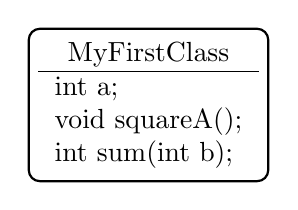
\begin{tikzpicture}
      \classbox{MyFirstClass}{
        int a; \\
        void squareA(); \\
        int sum(int b);
      }
    \end{tikzpicture}
    \vfill \null
  \end{multicols}
\end{frame}

\begin{frame}[fragile]
  \frametitlecpp[98]{Separating the interface}
  \begin{columns}[t]
    \begin{column}{.45\textwidth}
    \begin{block}{Header: MyClass.hpp}
      \begin{cppcode*}{gobble=4}
        #pragma once
        struct MyClass {
          int a;
          void squareA();
        };
      \end{cppcode*}
    \end{block}
    \begin{block}{Implementation: MyClass.cpp}
      \begin{cppcode*}{gobble=4}
        #include "MyClass.hpp"
        void MyClass::squareA() {
          a *= a;
        }
      \end{cppcode*}
    \end{block}
    \end{column}
    \begin{column}{.45\textwidth}
    \begin{block}{User 1: main.cpp}
      \begin{cppcode*}{gobble=4}
        #include "MyClass.hpp"
        int main() {
          MyClass mc;
          ...
        }
      \end{cppcode*}
    \end{block}
    \begin{block}{User 2: fun.cpp}
      \begin{cppcode*}{gobble=4}
        #include "MyClass.hpp"
        void f(MyClass& mc) {
          mc.squareA();
        }
      \end{cppcode*}
    \end{block}
    \end{column}
  \end{columns}
\end{frame}

\begin{frame}[fragile]
  \frametitlecpp[98]{Implementing methods}
  \begin{goodpractice}{Implementing methods}
    \begin{itemize}
    \item usually in .cpp, outside of class declaration
    \item using the class name as ``namespace''
    \item short member functions can be in the header
    \item some functions (templates, \cppinline{constexpr}) must be in the header
    \end{itemize}
  \end{goodpractice}
  \begin{block}{}
    \begin{cppcode}
    #include "MyFirstClass.hpp"

    void MyFirstClass::squareA() {
      a *= a;
    }
    int MyFirstClass::sum(int b) {
      return a + b;
    }
    \end{cppcode}
  \end{block}
\end{frame}

\begin{frame}[fragile]
  \frametitlecpp[98]{Method overloading}
  \begin{block}{The rules in \cpp}
    \begin{itemize}
    \item overloading is authorized and welcome
    \item signature is part of the method identity
    \item but not the return type
    \end{itemize}
  \end{block}
  \begin{cppcode}
    struct MyFirstClass {
      int a;
      int sum(int b);
      int sum(int b, int c);
    };

    int MyFirstClass::sum(int b) { return a + b; }

    int MyFirstClass::sum(int b, int c) {
      return a + b + c;
    }
  \end{cppcode}
\end{frame}

\subsection[inherit]{Inheritance}

\begin{frame}[fragile]
  \frametitlecpp[98]{First inheritance}
  \begin{multicols}{2}
    \begin{cppcode*}{gobble=2}
      struct MyFirstClass {
        int a;
        void squareA() { a *= a; }
      };
      struct MySecondClass :
        MyFirstClass {
        int b;
        int sum() { return a + b; }
      };

      MySecondClass myObj2;
      myObj2.a = 2;
      myObj2.b = 5;
      myObj2.squareA();
      int i = myObj2.sum(); // i = 9
    \end{cppcode*}
    \columnbreak
    \raggedleft
    \null \vfill
    \begin{overprint}[0.8\columnwidth]
      \onslide<1>
      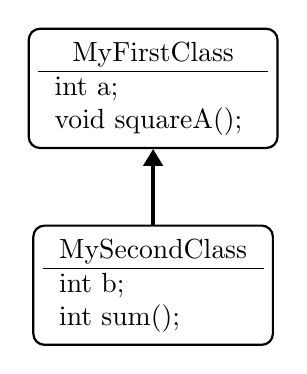
\begin{tikzpicture}[node distance=2.5cm]
        \classbox{MyFirstClass}{
          int a; \\
          void squareA();
        }
        \classbox[below of=MyFirstClass]{MySecondClass}{
          int b; \\
          int sum();
        }
        \draw[very thick,-Triangle] (MySecondClass)--(MyFirstClass);
      \end{tikzpicture}
      \onslide<2>
      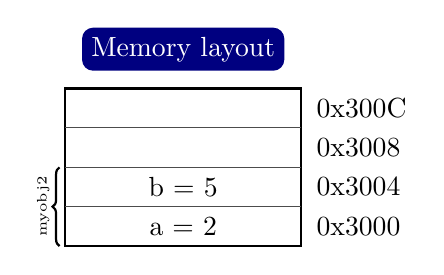
\begin{tikzpicture}
        \memorystack[size x=3cm,word size=1,block size=4,nb blocks=4]
        \memorypush{a = 2}
        \memorypush{b = 5}
        \memorystruct{1}{2}{\tiny myobj2}
      \end{tikzpicture}
    \end{overprint}
    \vfill \null
  \end{multicols}
\end{frame}

\begin{frame}[fragile]
  \frametitlecpp[98]{Managing access to class members}
  \begin{block}{\texttt{public} / \texttt{private} keywords}
    \begin{description}
      \item[\texttt{private}] allows access only within the class
      \item[\texttt{public}] allows access from anywhere
    \end{description}
    \begin{itemize}
       \item The default for \texttt{class} is \cppinline{private}
       \item The default for \texttt{struct} is \cppinline{public}
    \end{itemize}
  \end{block}
  \begin{multicols}{2}
    \begin{cppcode*}{gobble=2}
      class MyFirstClass {
      public:
        void setA(int x);
        int getA();
        void squareA();
      private:
        int a;
      };
    \end{cppcode*}
    \columnbreak
    \begin{cppcode*}{gobble=2,firstnumber=9}
      MyFirstClass obj;
      obj.a = 5;   // error !
      obj.setA(5); // ok
      obj.squareA();
      int b = obj.getA();
    \end{cppcode*}
    \pause
    \begin{tcolorbox}[left=0mm,right=0mm,top=0mm,bottom=0mm,colback=red!5!white,colframe=red!75!black]
      This breaks MySecondClass !
    \end{tcolorbox}
  \end{multicols}
\end{frame}

\begin{frame}[fragile]
  \frametitlecpp[98]{Managing access to class members(2)}
  \begin{block}{Solution is \texttt{protected} keyword}
    Gives access to classes inheriting from base class
  \end{block}
  \begin{multicols}{2}
    \begin{cppcode*}{gobble=2}
      class MyFirstClass {
      public:
        void setA(int a);
        int getA();
        void squareA();
      protected:
        int a;
      };
    \end{cppcode*}
    \columnbreak
    \begin{cppcode*}{gobble=2,firstnumber=13}
      class MySecondClass :
        public MyFirstClass {
      public:
        int sum() {
          return a + b;
        }
      private:
        int b;
      };
    \end{cppcode*}
  \end{multicols}
\end{frame}

\begin{frame}[fragile]
  \frametitlecpp[98]{Managing inheritance privacy}
  \begin{block}{Inheritance can be public, protected or private}
    It influences the privacy of inherited members for external code.\\
    The code of the class itself is not affected
    \begin{description}
    \item[\texttt{public}] privacy of inherited members remains unchanged
    \item[\texttt{protected}] inherited public members are seen as protected
    \item[\texttt{private}] all inherited members are seen as private \\
      this is the default for classes if nothing is specified
    \end{description}
  \end{block}
  \pause
  \begin{block}{Net result for external code}
    \begin{itemize}
    \item only public members of public inheritance are accessible
    \end{itemize}
  \end{block}
  \begin{block}{Net result for code in derived classes}
    \begin{itemize}
    \item only public and protected members of public and protected parents are accessible
    \end{itemize}
  \end{block}
\end{frame}

\begin{frame}[fragile]
  \frametitlecpp[98]{Managing inheritance privacy - public}
  \begin{multicols}{2}
    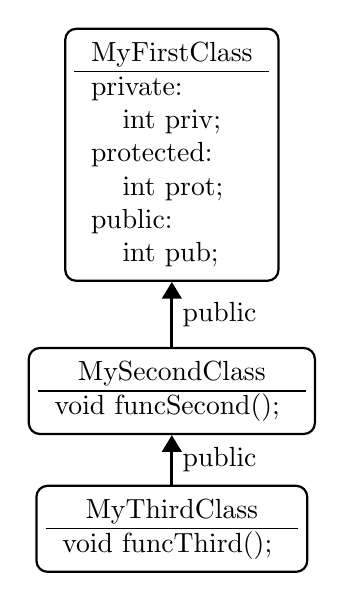
\begin{tikzpicture}[node distance=3cm]
      \classbox{MyFirstClass}{
      private: \\
        \hspace{0.4cm}int priv; \\
      protected: \\
        \hspace{0.4cm}int prot; \\
      public: \\
        \hspace{0.4cm}int pub;
      }
      \classbox[below of=MyFirstClass]{MySecondClass}{
        void funcSecond();
      }
      \classbox[below of=MySecondClass,node distance=1.75cm]{MyThirdClass}{
        void funcThird();
      }
      \draw[very thick,-Triangle] (MySecondClass)--(MyFirstClass) node[midway,right] {public};
      \draw[very thick,-Triangle] (MyThirdClass)--(MySecondClass) node[midway,right] {public};
    \end{tikzpicture}
    \columnbreak
    \begin{cppcode*}{gobble=2}
      void funcSecond() {
        int a = priv;   // Error
        int b = prot;   // OK
        int c = pub;    // OK
      }
      void funcThird() {
        int a = priv;   // Error
        int b = prot;   // OK
        int c = pub;    // OK
      }
      void extFunc(MyThirdClass t) {
        int a = t.priv; // Error
        int b = t.prot; // Error
        int c = t.pub;  // OK
      }
    \end{cppcode*}
  \end{multicols}
\end{frame}

\begin{frame}[fragile]
  \frametitlecpp[98]{Managing inheritance privacy - protected}
  \begin{multicols}{2}
    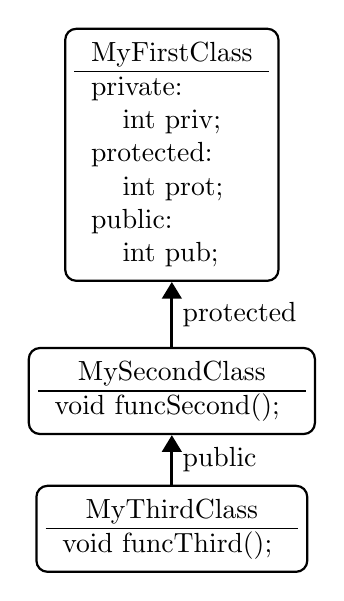
\begin{tikzpicture}[node distance=3cm]
      \classbox{MyFirstClass}{
      private: \\
        \hspace{0.4cm}int priv; \\
      protected: \\
        \hspace{0.4cm}int prot; \\
      public: \\
        \hspace{0.4cm}int pub;
      }
      \classbox[below of=MyFirstClass]{MySecondClass}{
        void funcSecond();
      }
      \classbox[below of=MySecondClass,node distance=1.75cm]{MyThirdClass}{
        void funcThird();
      }
      \draw[very thick,-Triangle] (MySecondClass)--(MyFirstClass) node[midway,right] {protected};
      \draw[very thick,-Triangle] (MyThirdClass)--(MySecondClass) node[midway,right] {public};
    \end{tikzpicture}
    \columnbreak
    \begin{cppcode*}{gobble=2,highlightlines=14}
      void funcSecond() {
        int a = priv;   // Error
        int b = prot;   // OK
        int c = pub;    // OK
      }
      void funcThird() {
        int a = priv;   // Error
        int b = prot;   // OK
        int c = pub;    // OK
      }
      void extFunc(MyThirdClass t) {
        int a = t.priv; // Error
        int b = t.prot; // Error
        int c = t.pub;  // Error
      }
    \end{cppcode*}
  \end{multicols}
\end{frame}

\begin{frame}[fragile]
  \frametitlecpp[98]{Managing inheritance privacy - private}
  \begin{multicols}{2}
    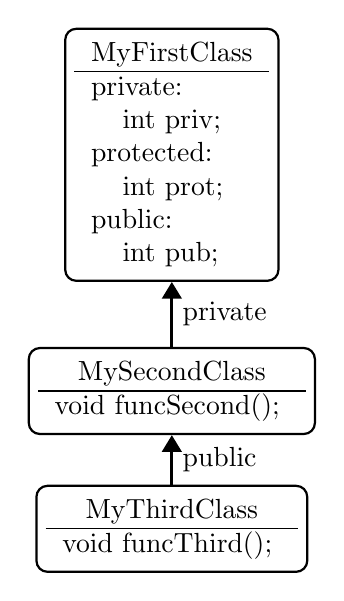
\begin{tikzpicture}[node distance=3cm]
      \classbox{MyFirstClass}{
      private: \\
        \hspace{0.4cm}int priv; \\
      protected: \\
        \hspace{0.4cm}int prot; \\
      public: \\
        \hspace{0.4cm}int pub;
      }
      \classbox[below of=MyFirstClass]{MySecondClass}{
        void funcSecond();
      }
      \classbox[below of=MySecondClass,node distance=1.75cm]{MyThirdClass}{
        void funcThird();
      }
      \draw[very thick,-Triangle] (MySecondClass)--(MyFirstClass) node[midway,right] {private};
      \draw[very thick,-Triangle] (MyThirdClass)--(MySecondClass) node[midway,right] {public};
    \end{tikzpicture}
    \columnbreak
    \begin{cppcode*}{gobble=2,highlightlines=8-9}
      void funcSecond() {
        int a = priv;   // Error
        int b = prot;   // OK
        int c = pub;    // OK
      }
      void funcThird() {
        int a = priv;   // Error
        int b = prot;   // Error
        int c = pub;    // Error
      }
      void extFunc(MyThirdClass t) {
        int a = t.priv; // Error
        int b = t.prot; // Error
        int c = t.pub;  // Error
      }
    \end{cppcode*}
  \end{multicols}
\end{frame}

\begin{advanced}
\begin{frame}[fragile]
  \frametitlecpp[11]{Final class}
  \begin{block}{Idea}
    \begin{itemize}
    \item make sure you cannot inherit from a given class
    \item by declaring it final
    \end{itemize}
  \end{block}
  \begin{exampleblock}{Practically}
    \begin{cppcode}
      struct Base final {
        ...
      };
      struct Derived : Base { // compiler error
        ...
      };
    \end{cppcode}
  \end{exampleblock}
\end{frame}
\end{advanced}

\subsection[construct]{Constructors/destructors}

\begin{frame}[fragile]
  \frametitlecpp[98]{Class Constructors and Destructors}
  \begin{block}{Concept}
    \begin{itemize}
    \item special functions called when building/destroying an object
    \item a class can have several constructors, but only one destructor
    \item the constructors have the same name as the class
    \item same for the destructor with a leading \mintinline{cpp}{~}
    \end{itemize}
  \end{block}
  \begin{multicols}{2}
    \begin{cppcode*}{gobble=2}
      class MyFirstClass {
      public:
        MyFirstClass();
        MyFirstClass(int a);
        ~MyFirstClass();
        ...
      protected:
        int a;
      };
    \end{cppcode*}
    \columnbreak
    \begin{cppcode*}{gobble=2,firstnumber=10}
      // note special notation for
      // initialization of members
      MyFirstClass() : a(0) {}

      MyFirstClass(int a_):a(a_) {}

      ~MyFirstClass() {}
    \end{cppcode*}
  \end{multicols}
\end{frame}


\begin{frame}[fragile]
  \frametitlecpp[98]{Class Constructors and Destructors}
  \begin{cppcode}
    class Vector {
    public:
      Vector(int n);
      ~Vector();
      void setN(int n, int value);
      int getN(int n);
    private:
      int len;
      int* data;
    };
    Vector::Vector(int n) : len(n) {
      data = new int[n];
    }
    Vector::~Vector() {
      delete[] data;
    }
  \end{cppcode}
\end{frame}

\begin{frame}[fragile]
  \frametitlecpp[98]{Constructors and inheritance}
  \begin{cppcode}
    struct MyFirstClass {
      int a;
      MyFirstClass();
      MyFirstClass(int a);
    };
    struct MySecondClass : MyFirstClass {
      int b;
      MySecondClass();
      MySecondClass(int b);
      MySecondClass(int a, int b);
    };
    MySecondClass::MySecondClass() : MyFirstClass(), b(0) {}
    MySecondClass::MySecondClass(int b_)
      : MyFirstClass(), b(b_) {}
    MySecondClass::MySecondClass(int a_, int b_)
      : MyFirstClass(a_), b(b_) {}
  \end{cppcode}
\end{frame}

\begin{frame}[fragile]
  \frametitlecpp[98]{Copy constructor}
  \begin{block}{Concept}
    \begin{itemize}
    \item special constructor called for replicating an object
    \item takes a single parameter of type \mintinline{cpp}{const &} to class
    \item provided by the compiler if not declared by the user
    \item in order to forbid copy, use \mintinline{cpp}{= delete} (see next slides)
      \begin{itemize}
      \item or private copy constructor with no implementation in \cpp98
      \end{itemize}
    \end{itemize}
  \end{block}
  \pause
  \begin{cppcode}
    struct MySecondClass : MyFirstClass {
      MySecondClass();
      MySecondClass(const MySecondClass &other);
    };
  \end{cppcode}
  \pause
  \begin{exampleblock}{The rule of 3/5/0 (\cpp98/\cpp11 and newer) - {\color{blue!50!white} \href{https://en.cppreference.com/w/cpp/language/rule_of_three}{cppreference}}}
    \begin{itemize}
    \item if a class has a destructor, a copy/move constructor or a copy/move assignment operator, it should have all three/five. strive for having none by using RAII types as members.
    \end{itemize}
  \end{exampleblock}
\end{frame}

\begin{frame}[fragile]
  \frametitlecpp[98]{Class Constructors and Destructors}
  \begin{cppcode}
    class Vector {
    public:
      Vector(int n);
      Vector(const Vector &other);
      ~Vector();
      ...
    };
    Vector::Vector(int n) : len(n) {
      data = new int[n];
    }
    Vector::Vector(const Vector &other) : len(other.len) {
      data = new int[len];
      std::copy(other.data, other.data + len, data);
    }
    Vector::~Vector() { delete[] data; }
  \end{cppcode}
\end{frame}

\begin{frame}[fragile]
  \frametitlecpp[98]{Explicit unary constructor}
  \begin{block}{Concept}
    \begin{itemize}
    \item A constructor with a single non-default parameter can be used by the compiler for an implicit conversion.
    \end{itemize}
  \end{block}
  \begin{cppcode}
    void print( const Vector & v )
      std::cout<<"printing v elements...\n";
    }

    int main {
      // calls Vector::Vector(int n) to construct a Vector
      // then calls print with that Vector
      print(3);
    };
  \end{cppcode}
\end{frame}

\begin{frame}[fragile]
  \frametitlecpp[98]{Explicit unary constructor}
  \begin{block}{Concept}
    \begin{itemize}
      \item The keyword \mintinline{cpp}{explicit} forbids such implicit conversions.
      \item It is recommended to use it systematically, except in special cases.
    \end{itemize}
  \end{block}
  \begin{cppcode}
    class Vector {
    public:
      explicit Vector(int n);
      Vector(const Vector &other);
      ~Vector();
      ...
    };
  \end{cppcode}
\end{frame}

\begin{frame}[fragile]
  \frametitlecpp[11]{Defaulted Constructor}
  \begin{block}{Idea}
    \begin{itemize}
    \item avoid empty default constructors like \mintinline{cpp}{ClassName() {}}
    \item declare them as \mintinline{cpp}{= default}
    \end{itemize}
  \end{block}
  \begin{block}{Details}
    \begin{itemize}
    \item without a user-defined constructor, a default one is provided
    \item any user-defined constructor disables the default one
    \item but the default one can be requested explicitly
    \item rule can be more subtle depending on data members
    \end{itemize}
  \end{block}
  \begin{exampleblock}{Practically}
    \begin{cppcode}
      Class() = default; // provide default if possible
      Class() = delete;  // disable default constructor
    \end{cppcode}
  \end{exampleblock}
\end{frame}

\begin{frame}[fragile]
  \frametitlecpp[11]{Delegating constructor}
  \begin{block}{Idea}
    \begin{itemize}
    \item avoid replication of code in several constructors
    \item by delegating to another constructor, in the initialization list
    \end{itemize}
  \end{block}
  \begin{exampleblock}{Practically}
    \begin{cppcode}
      struct Delegate {
        int m_i;
        Delegate(int i) : m_i(i) {
          ... complex initialization ...
        }
        Delegate() : Delegate(42) {}
      };
    \end{cppcode}
  \end{exampleblock}
\end{frame}

\begin{frame}[fragile]
  \frametitlecpp[11]{Constructor inheritance}
  \begin{block}{Idea}
    \begin{itemize}
    \item avoid having to re-declare parent's constructors
    \item by stating that we inherit all parent constructors
    \end{itemize}
  \end{block}
  \begin{exampleblock}{Practically}
    \begin{cppcode}
      struct BaseClass {
        BaseClass(int value);
      };
      struct DerivedClass : BaseClass {
        using BaseClass::BaseClass;
      };
      DerivedClass a{5};
    \end{cppcode}
  \end{exampleblock}
\end{frame}

\begin{frame}[fragile]
  \frametitlecpp[11]{Member initialization}
  \begin{block}{Idea}
    \begin{itemize}
    \item avoid redefining same default value for members n times
    \item by defining it once at member declaration time
    \end{itemize}
  \end{block}
  \begin{exampleblock}{Practically}
    \begin{cppcode}
      struct BaseClass {
        int a{5}; // also possible: int a = 5;
        BaseClass() = default;
        BaseClass(int _a) : a(_a) {}
      };
      struct DerivedClass : BaseClass {
        int b{6};
        using BaseClass::BaseClass;
      };
      DerivedClass d{7}; // a = 7, b = 6
    \end{cppcode}
  \end{exampleblock}
\end{frame}

\begin{frame}[fragile]
  \frametitlecpp[11]{Calling constructors}
  \begin{block}{After object declaration, arguments within \{\}}
    \begin{cppcode*}{gobble=2}
      struct A {
        int a;
        float b;
        A();
        A(int);
        A(int, int);
      };

      A a{1,2};    // A::A(int, int)
      A a{1};      // A::A(int)
      A a{};       // A::A()
      A a;         // A::A()
      A a = {1,2}; // A::A(int, int)
    \end{cppcode*}
  \end{block}
\end{frame}

\begin{frame}[fragile]
  \frametitlecpp[98]{Calling constructors the old way}
  \begin{block}{Arguments are given within (), aka \cpp98 nightmare}
    \begin{cppcode*}{gobble=2}
      struct A {
        int a;
        float b;
        A();
        A(int);
        A(int, int);
      };

      A a(1,2);    // A::A(int, int)
      A a(1);      // A::A(int)
      A a();       // declaration of a function !
      A a;         // A::A()
      A a = (1,2); // A::A(int), comma operator !
      A a = {1,2}; // not allowed
    \end{cppcode*}
  \end{block}
\end{frame}

\begin{frame}[fragile]
  \frametitlecpp[11]{Calling constructors for arrays and vectors}
  \begin{exampleblock}{list of items given within \{\}}
    \begin{cppcode*}{firstnumber=10}
     int ip[3]{1,2,3};
     int* ip = new int[3]{1,2,3};
     std::vector<int> v{1,2,3};
    \end{cppcode*}
  \end{exampleblock}
  \pause
  \begin{block}{\cpp98 nightmare}
    \begin{cppcode*}{firstnumber=10}
     int ip[3]{1,2,3};            // OK
     int* ip = new int[3]{1,2,3}; // not allowed
     std::vector<int> v{1,2,3};   // not allowed
    \end{cppcode*}
  \end{block}
\end{frame}

\subsection[static]{Static members}

\begin{frame}[fragile]
  \frametitlecpp[98]{Static members}
  \begin{block}{Concept}
    \begin{itemize}
    \item members attached to a class rather than to an object
    \item usable with or without an instance of the class
    \item identified by the \cppinline{static} keyword
    \end{itemize}
  \end{block}
  \begin{cppcode}
    class Text {
    public:
      static std::string upper(std::string) {...}
    private:
      static int callsToUpper; // add `inline` in C++17
    };
    int Text::callsToUpper = 0; // required before C++17
    std::string uppers = Text::upper("my text");
    // now Text::callsToUpper is 1
  \end{cppcode}
\end{frame}

\subsection[new]{Allocating objects}

\begin{frame}[fragile]
  \frametitlecpp[98]{Process memory organization}
  \begin{block}{4 main areas}
    \begin{description}
    \item[the code segment] for the machine code of the executable
    \item[the data segment] for global variables
    \item[the heap] for dynamically allocated variables
    \item[the stack] for parameters of functions and local variables
    \end{description}
  \end{block}
  \hspace{2.5cm}
  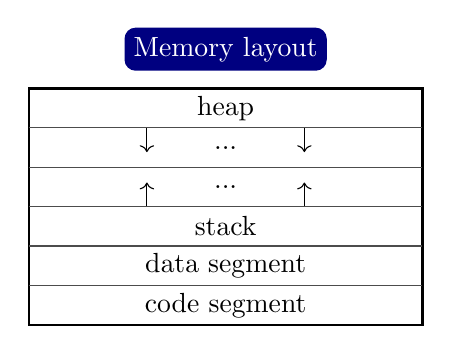
\begin{tikzpicture}
    \memorystack[size x=5cm,word size=1,nb blocks=6,addresses=0]
    \memorypush{code segment}
    \memorypush{data segment}
    \memorypush{stack}
    \memorypush{...}
    \memorypush{...}
    \memorypush{heap}
    \draw[->] (stack3-1.north) ++(-1cm,0) -- +(0,.3cm);
    \draw[->] (stack3-1.north) ++(1cm,0) -- +(0,.3cm);
    \draw[->] (stack6-1.south) ++(-1cm,0) -- +(0,-.3cm);
    \draw[->] (stack6-1.south) ++(1cm,0) -- +(0,-.3cm);
  \end{tikzpicture}
\end{frame}

\begin{frame}[fragile]
  \frametitlecpp[98]{The Stack}
  \begin{block}{Main characteristics}
    \begin{itemize}
    \item allocation on the stack stays valid for the duration of the current scope.
    It is destroyed when it is popped off the stack.
    \item memory allocated on the stack is known at compile time and can thus be accessed through a variable.
    \item the stack is relatively small, it is not a good idea to allocate large arrays, structures or classes
    \item each thread in a process has its own stack
      \begin{itemize}
      \item allocations on the stack are thus ``thread private''
      \item and do not introduce any thread safety issues
      \end{itemize}
    \end{itemize}
  \end{block}
\end{frame}

\begin{frame}[fragile]
  \frametitlecpp[98]{Object allocation on the stack}
  \begin{block}{On the stack}
    \begin{itemize}
    \item objects are created when declared (constructor called)
    \item objects are destructed when out of scope (destructor is called)
    \end{itemize}
  \end{block}
  \begin{cppcode}
    int f() {
      MyFirstClass a{3}; // constructor called
      ...
    } // destructor called

    int g() {
      MyFirstClass a; // default constructor called
      ...
    }  // destructor called
  \end{cppcode}
\end{frame}

\begin{frame}[fragile]
  \frametitlecpp[98]{The Heap}
  \begin{block}{Main characteristics}
    \begin{itemize}
    \item Allocated memory stays allocated until it is specifically deallocated
      \begin{itemize}
      \item beware memory leaks
      \end{itemize}
    \item Dynamically allocated memory must be accessed through pointers
    \item large arrays, structures, or classes should be allocated here
    \item there is a single, shared heap per process
      \begin{itemize}
      \item allows to share data between threads
      \item introduces race conditions and thread safety issues!
      \end{itemize}
    \end{itemize}
  \end{block}
\end{frame}

\begin{frame}[fragile]
  \frametitlecpp[98]{Object allocation on the heap}
  \begin{block}{On the heap}
    \begin{itemize}
    \item objects are created by calling \cppinline{new} (constructor is called)
    \item objects are destructed by calling \cppinline{delete} (destructor is called)
    \end{itemize}
  \end{block}
  \begin{cppcode}
    int f() {
      // default constructor called
      MyFirstClass *a = new MyFirstClass;
      delete a; // destructor is called
    }
    int g() {
      // constructor called
      MyFirstClass *a = new MyFirstClass(3);
    } // memory leak !!!
  \end{cppcode}
  \begin{goodpracticeWithShortcut}{Prefer smart pointers over new/delete}{Prefer smart pointer}
    Prefer smart pointers to manage objects (discussed later)
  \end{goodpracticeWithShortcut}
\end{frame}

\begin{frame}[fragile]
  \frametitlecpp[98]{Array allocation on the heap}
  \begin{block}{Arrays on the heap}
    \begin{itemize}
    \item arrays of objects are created by calling \cppinline{new[]} \\
      default constructor is called for each object of the array
    \item arrays of object are destructed by calling \cppinline{delete[]} \\
      destructor is called for each object of the array
    \end{itemize}
  \end{block}
  \begin{cppcode}
    int f() {
      // default constructor called 10 times
      MyFirstClass *a = new MyFirstClass[10];
      ...
      delete[] a; // destructor called 10 times
    }
  \end{cppcode}
  \begin{goodpracticeWithShortcut}{Prefer containers over new-ed arrays}{Prefer containers}
    Prefer containers to manage collections of objects (discussed later)
  \end{goodpracticeWithShortcut}
\end{frame}

\subsection[advOO]{Advanced OO}

\begin{frame}[fragile]
  \frametitlecpp[98]{Polymorphism}
  \begin{block}{the concept}
    \begin{itemize}
    \item objects actually have multiple types simultaneously
    \item and can be used as any of them
    \end{itemize}
  \end{block}
  \begin{multicols}{2}
    \begin{cppcode*}{gobble=2}
      Polygon p;

      int f(Drawable & d) {...}
      f(p);  //ok

      try {
        throw p;
      } catch (Shape & e) {
        // will be caught
      }
    \end{cppcode*}
    \columnbreak
    \center
    \begin{overprint}
      \onslide<1>
      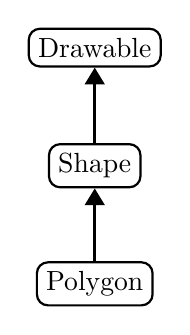
\begin{tikzpicture}[node distance=1.5cm]
        \classbox{Drawable}{}
        \classbox[below of=Drawable]{Shape}{}
        \classbox[below of=Shape]{Polygon}{}
        \draw[very thick,-Triangle] (Polygon) -- (Shape);
        \draw[very thick,-Triangle] (Shape) -- (Drawable);
      \end{tikzpicture}
      \onslide<2->
      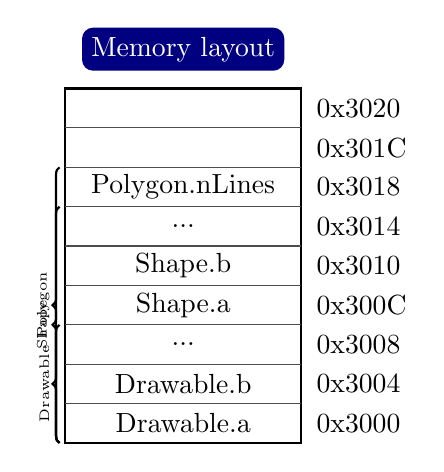
\begin{tikzpicture}
        \memorystack[size x=3cm,word size=1,block size=4,nb blocks=9]
        \memorypush{Drawable.a}
        \memorypush{Drawable.b}
        \memorypush{...}
        \memorypush{Shape.a}
        \memorypush{Shape.b}
        \memorypush{...}
        \memorypush{Polygon.nLines}
        \onslide<2>{\memorystruct{1}{7}{\tiny Polygon}}
        \onslide<3>{\memorystruct{1}{3}{\tiny Drawable}}
        \onslide<4>{\memorystruct{1}{6}{\tiny Shape}}
      \end{tikzpicture}
    \end{overprint}
  \end{multicols}
\end{frame}


\begin{frame}[fragile]
  \frametitlecpp[98]{Inheritance privacy and polymorphism}
  \begin{block}{Only public base classes are visible to outside code}
    \begin{itemize}
    \item private and protected bases are not
    \item this may restrict usage of polymorphism
    \end{itemize}
  \end{block}
  \begin{multicols}{2}
    \begin{cppcode*}{gobble=2}
      Polygon p;

      int f(Drawable & d) {...}
      f(p);  // Not ok anymore

      try {
        throw p;
      } catch (Shape & e) {
        // ok, will be caught
      }
    \end{cppcode*}
    \columnbreak
    \center
    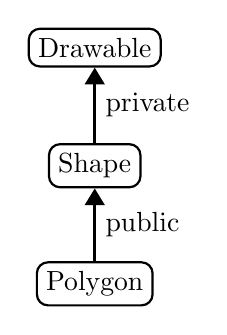
\begin{tikzpicture}[node distance=1.5cm]
      \classbox{Drawable}{}
      \classbox[below of=Drawable]{Shape}{}
      \classbox[below of=Shape]{Polygon}{}
      \draw[very thick,-Triangle] (Polygon) -- (Shape) node[midway,right] {public};
      \draw[very thick,-Triangle] (Shape) -- (Drawable) node[midway,right] {private};
    \end{tikzpicture}
  \end{multicols}
\end{frame}

\begin{frame}[fragile]
  \frametitlecpp[98]{Method overriding}
  \begin{block}{the idea}
    \begin{itemize}
    \item a method of the parent class can be replaced in a derived class
    \item but which one is called?
    \end{itemize}
  \end{block}
  \begin{multicols}{2}
    \begin{cppcode*}{gobble=2}
      Polygon p;
      p.draw(); // ?

      Shape & s = p;
      s.draw(); // ?
    \end{cppcode*}
    \columnbreak
    \center
    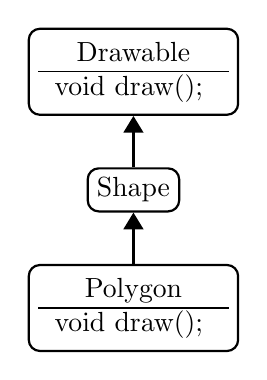
\begin{tikzpicture}[node distance=1.5cm]
      \classbox{Drawable}{
        void draw();
      }
      \classbox[below of=Drawable]{Shape}{}
      \classbox[below of=Shape]{Polygon}{
        void draw();
      }
      \draw[very thick,-Triangle] (Polygon) -- (Shape);
      \draw[very thick,-Triangle] (Shape) -- (Drawable);
    \end{tikzpicture}
  \end{multicols}
\end{frame}

\begin{frame}[fragile]
  \frametitlecpp[98]{Virtual methods}
  \begin{block}{the concept}
    \begin{itemize}
    \item methods can be declared \cppinline{virtual}
    \item for these, the most derived object's implementation is used
          (i.e.\ the dynamic type behind a pointer/reference)
    \item for non-virtual methods, the static type of the variable decides
    \end{itemize}
  \end{block}
  \begin{overprint}
  \onslide<2>
  \begin{multicols}{2}
    \begin{cppcode*}{gobble=2}
      Polygon p;
      p.draw(); // Polygon.draw

      Shape & s = p;
      s.draw(); // Drawable.draw
    \end{cppcode*}
    \columnbreak
    \center
    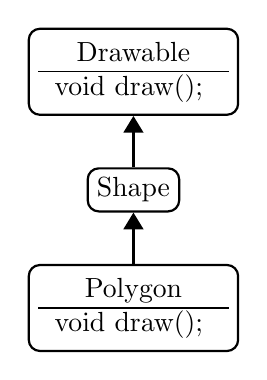
\begin{tikzpicture}[node distance=1.5cm]
      \classbox{Drawable}{
        \cppinline{void draw();}
      }
      \classbox[below of=Drawable]{Shape}{}
      \classbox[below of=Shape]{Polygon}{
        \cppinline{void draw();}
      }
      \draw[very thick,-Triangle] (Polygon) -- (Shape);
      \draw[very thick,-Triangle] (Shape) -- (Drawable);
    \end{tikzpicture}
  \end{multicols}

  \onslide<3>
    \begin{multicols}{2}
    \begin{cppcode*}{gobble=2,highlightlines=5}
      Polygon p;
      p.draw(); // Polygon.draw

      Shape & s = p;
      s.draw(); // Polygon.draw
    \end{cppcode*}
    \columnbreak
    \center
    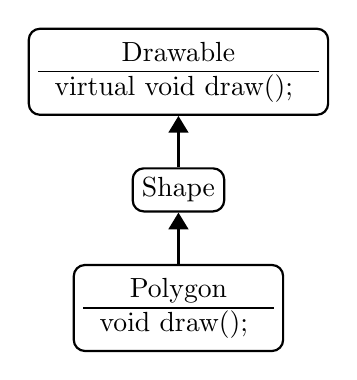
\begin{tikzpicture}[node distance=1.5cm]
      \classbox{Drawable}{
        \cppinline{virtual void draw();}
      }
      \classbox[below of=Drawable]{Shape}{}
      \classbox[below of=Shape]{Polygon}{
        \cppinline{void draw();}
      }
      \draw[very thick,-Triangle] (Polygon) -- (Shape);
      \draw[very thick,-Triangle] (Shape) -- (Drawable);
    \end{tikzpicture}
  \end{multicols}
  \end{overprint}
\end{frame}

\begin{frame}[fragile]
  \frametitlecpp[11]{Virtual methods - implications}
  \begin{block}{Mechanics}
    \begin{itemize}
    \item virtual methods are dispatched at run time
      \begin{itemize}
      \item while non-virtual methods are bound at compile time
      \end{itemize}
    \item they also imply extra storage and an extra indirection
      \begin{itemize}
      \item practically, the object stores a pointer to the correct method
      \item in a so-called ``virtual table'' (``vtable'')
      \end{itemize}
    \end{itemize}
  \end{block}
  \begin{alertblock}{Consequences}
    \begin{itemize}
    \item virtual methods are ``slower'' than standard ones
    \item and they can rarely be inlined
    \item templates are an alternative for performance-critical cases
    \end{itemize}
  \end{alertblock}
\end{frame}

\begin{frame}[fragile]
  \frametitlecpp[11]{{\texttt override} keyword}
  \begin{block}{Principle}
    \begin{itemize}
    \item when overriding a virtual method
    \item the \cppinline|override| keyword should be used
    \item the \cppinline|virtual| keyword is then optional
    \end{itemize}
  \end{block}
  \begin{exampleblock}{Practically}
    \begin{cppcode}
      struct Base {
        virtual void some_func(float);
      };
      struct Derived : Base {
        void some_func(float) override;
      };
    \end{cppcode}
  \end{exampleblock}
\end{frame}

\begin{frame}[fragile]
  \frametitlecpp[11]{Why was {\texttt override} keyword introduced?}
  To detect the mistake in the following code :
  \begin{block}{Without {\texttt override} (\cpp98)}
    \begin{cppcode}
      struct Base {
        virtual void some_func(float);
      };
      struct Derived : Base {
        void some_func(double); // oops !
      };
    \end{cppcode}
  \end{block}
  \begin{itemize}
  \item with \cppinline|override|, you would get a compiler error
  \item if you forget \cppinline|override| when you should have it, you get a compiler warning
  \end{itemize}
\end{frame}

\begin{advanced}
\begin{frame}[fragile]
  \frametitlecpp[11]{{\texttt final} keyword}
  \begin{block}{Idea}
    \begin{itemize}
    \item make sure you cannot further override a given virtual method
    \item by declaring it final
    \end{itemize}
  \end{block}
  \begin{exampleblock}{Practically}
    \begin{cppcode}
      struct Base {
        virtual void some_func(float);
      };
      struct Intermediate : Base {
        void some_func(float) final;
      };
      struct Derived : Intermediate {
        void some_func(float) override; // error
      };
    \end{cppcode}
  \end{exampleblock}
\end{frame}
\end{advanced}

\begin{frame}[fragile]
  \frametitlecpp[98]{Pure Virtual methods}
  \begin{block}{Concept}
    \begin{itemize}
    \item unimplemented methods that must be overridden
    \item marked by \cppinline{= 0} in the declaration
    \item makes their class abstract
    \item only non-abstract classes can be instantiated
    \end{itemize}
  \end{block}
  \pause
  \begin{multicols}{2}
    \begin{cppcode*}{gobble=2}
      // Error : abstract class
      Shape s;

      // ok, draw has been implemented
      Polygon p;

      // Shape type still usable
      Shape & s = p;
      s.draw();
    \end{cppcode*}
    \columnbreak
    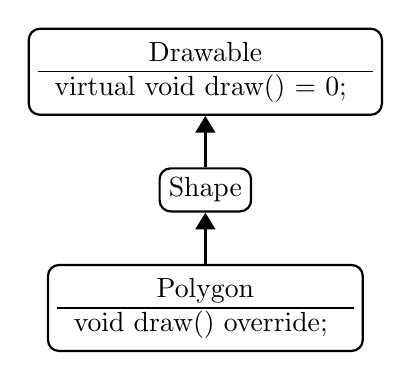
\begin{tikzpicture}[node distance=1.5cm]
      \classbox{Drawable}{
        \cppinline{virtual void draw() = 0;}
      }
      \classbox[below of=Drawable]{Shape}{}
      \classbox[below of=Shape]{Polygon}{
        \cppinline{void draw() override;}
      }
      \draw[very thick,-Triangle] (Polygon) -- (Shape);
      \draw[very thick,-Triangle] (Shape) -- (Drawable);
    \end{tikzpicture}
  \end{multicols}
\end{frame}

\begin{frame}[fragile]
  \frametitlecpp[98]{Polymorphism and destruction}
  \begin{block}{Owning base pointers}
    We sometimes need to maintain owning pointers to base classes:
  \end{block}
  \begin{overprint}
    \onslide<1>
  \begin{cppcode}
    struct Drawable {
       virtual void draw() = 0;
    };
    Drawable* getImpl();

    Drawable* p = getImpl();
    p->draw();
    delete p;
  \end{cppcode}
    \onslide<2>
  \begin{cppcode}
    struct Drawable {
       virtual void draw() = 0;
    };
    std::unique_ptr<Drawable> getImpl(); // better API

    auto p = getImpl();
    p->draw();
  \end{cppcode}
  \end{overprint}
  \begin{block}{}
    \begin{itemize}
      \item What happens when \cppinline{p} is deleted?
      \item What if a class deriving from \cppinline{Drawable} has a destructor?
    \end{itemize}
  \end{block}
\end{frame}

\begin{frame}[fragile]
  \frametitlecpp[98]{Polymorphism and destruction}
  \begin{block}{Virtual destructors}
    \begin{itemize}
    \item We can mark a destructor as \cppinline{virtual}
    \item This selects the right destructor based on the runtime type
    \end{itemize}
  \end{block}
  \begin{cppcode}
    struct Drawable {
       virtual ~Drawable() = default;
       virtual void draw() = 0;
    };
    Drawable* p = getImpl(); // returns derived obj.
    p->draw();
    delete p; // dynamic dispatch to right destructor
  \end{cppcode}
  \begin{goodpractice}{Virtual destructors}
    \begin{itemize}
      \item If you expect users to inherit from your class and override methods (i.e.\ use your class polymorphically), declare its destructor \cppinline{virtual}
    \end{itemize}
  \end{goodpractice}
\end{frame}

\begin{frame}[fragile]
  \frametitlecpp[98]{Pure Abstract Class aka Interface}
  \begin{block}{Definition of pure abstract class}
    \begin{itemize}
    \item a class that has
      \begin{itemize}
        \item no data members
        \item all its methods pure virtual
        \item a \cppinline{virtual} destructor
      \end{itemize}
    \item the equivalent of an Interface in Java
    \end{itemize}
  \end{block}
  \begin{multicols}{2}
    \begin{cppcode*}{gobble=2}
      struct Drawable {
        ~Drawable() = default;
        virtual void draw() = 0;
      }
    \end{cppcode*}
    \columnbreak
    \center
    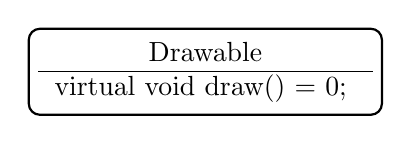
\begin{tikzpicture}[node distance=1.5cm]
      \classbox{Drawable}{
        virtual void draw() = 0;
      }
    \end{tikzpicture}
  \end{multicols}
\end{frame}

\begin{frame}[fragile]
  \frametitlecpp[98]{Overriding overloaded methods}
  \begin{block}{Concept}
    \begin{itemize}
    \item overriding an overloaded method will hide the others
    \item unless you inherit them using \cppinline{using}
    \end{itemize}
  \end{block}
  \begin{cppcode*}{gobble=0}
    struct BaseClass {
      virtual int foo(std::string);
      virtual int foo(int);
    };
    struct DerivedClass : BaseClass {
      using BaseClass::foo;
      int foo(std::string) override;
    };
    DerivedClass dc;
    dc.foo(4);      // error if no using
    \end{cppcode*}
\end{frame}

\begin{frame}[fragile]
  \frametitlecpp[98]{Polymorphism}
  \begin{exercise}{Polymorphism}
    \begin{itemize}
    \item go to code/polymorphism
    \item look at the code
    \item open trypoly.cpp
    \item create a Pentagon, call its perimeter method
    \item create a Hexagon, call its perimeter method
    \item create a Hexagon, call its parent's perimeter method
    \item retry with virtual methods
    \end{itemize}
  \end{exercise}
\end{frame}

\begin{frame}[fragile]
  \frametitlecpp[98]{Multiple Inheritance}
  \begin{block}{Concept}
    \begin{itemize}
    \item one class can inherit from multiple parents
    \end{itemize}
  \end{block}
  \begin{multicols}{2}
    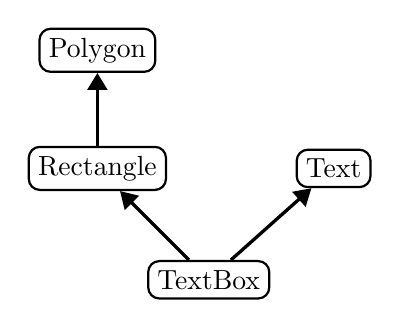
\begin{tikzpicture}[]
      \classbox[]{Polygon}{}
      \classbox[below of=Polygon,node distance=1.5cm]{Rectangle}{}
      \classbox[right of=Rectangle,node distance=3cm]{Text}{}
      \classbox[below right of=Rectangle,node distance=2cm]{TextBox}{}
      \draw[very thick,Triangle-] (Polygon) -- (Rectangle);
      \draw[very thick,Triangle-] (Rectangle) -- (TextBox);
      \draw[very thick,Triangle-] (Text) -- (TextBox);
    \end{tikzpicture}
    \columnbreak
    \vspace{2cm}
    \begin{cppcode*}{gobble=2}
      class TextBox :
        public Rectangle, Text {
        // inherits from both
        // publicly from Rectangle
        // privately from Text
      }
    \end{cppcode*}
  \end{multicols}
\end{frame}

\begin{frame}[fragile]
  \frametitlecpp[98]{The diamond shape}
  \begin{block}{Definition}
    \begin{itemize}
    \item situation when one class inherits several times from a given grand parent
    \end{itemize}
  \end{block}
  \begin{alertblock}{Problem}
    \begin{itemize}
    \item are the members of the grand parent replicated?
    \end{itemize}
  \end{alertblock}
  \vfill
  \hspace{2.5cm}
  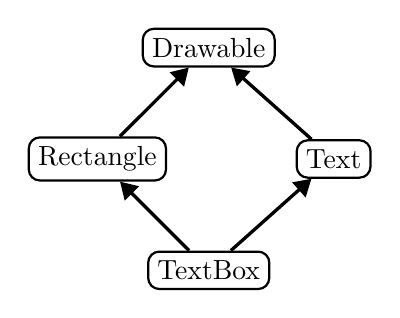
\begin{tikzpicture}[]
    \classbox[]{Drawable}{}
    \classbox[below left of=Drawable,node distance=2cm]{Rectangle}{}
    \classbox[right of=Rectangle,node distance=3cm]{Text}{}
    \classbox[below right of=Rectangle,node distance=2cm]{TextBox}{}
    \draw[very thick,Triangle-] (Drawable) -- (Rectangle);
    \draw[very thick,Triangle-] (Drawable) -- (Text);
    \draw[very thick,Triangle-] (Rectangle) -- (TextBox);
    \draw[very thick,Triangle-] (Text) -- (TextBox);
  \end{tikzpicture}
\end{frame}

\begin{frame}[fragile]
  \frametitlecpp[98]{Virtual inheritance}
  \begin{block}{Solution}
    \begin{itemize}
    \item inheritance can be \cppinline{virtual} or not
    \begin{itemize}
      \item \cppinline{virtual} inheritance will ``share'' parents
      \item standard inheritance will replicate them
    \end{itemize}
    \item most derived class will call the virtual base class's constructor
    \end{itemize}
    \begin{cppcode}
      class Text : public virtual Drawable {...};
      class Rectangle : public virtual Drawable {...};
    \end{cppcode}
  \end{block}
  \begin{multicols}{2}
    \begin{tikzpicture}[]
      \classbox[below of=title]{Drawable}{}
      \classbox[below left of=Drawable,node distance=2cm]{Rectangle}{}
      \classbox[right of=Rectangle,node distance=3cm]{Text}{}
      \classbox[below right of=Rectangle,node distance=2cm]{TextBox}{}
      \draw[very thick,Triangle-] (Drawable) -- node[below,pos=0.35,sloped] {\scriptsize virtual} (Rectangle);
      \draw[very thick,Triangle-] (Drawable) -- node[below,pos=0.45,sloped] {\scriptsize virtual} (Text);
      \draw[very thick,Triangle-] (Rectangle) -- (TextBox);
      \draw[very thick,Triangle-] (Text) -- (TextBox);
    \end{tikzpicture}
    \columnbreak
    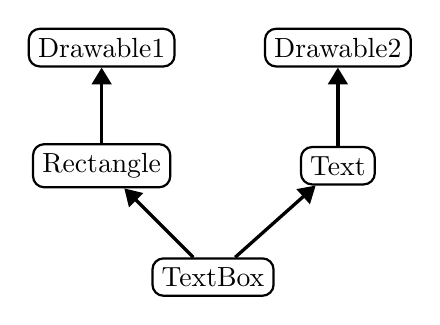
\begin{tikzpicture}[]
      \classbox[]{Drawable1}{}
      \classbox[below of=Drawable1,node distance=1.5cm]{Rectangle}{}
      \draw[very thick,Triangle-] (Drawable1) -- (Rectangle);
      \classbox[right of=Drawable1,node distance=3cm]{Drawable2}{}
      \classbox[below of=Drawable2,node distance=1.5cm]{Text}{}
      \draw[very thick,Triangle-] (Drawable2) -- (Text);
      \classbox[below right of=Rectangle,node distance=2cm]{TextBox}{}
      \draw[very thick,Triangle-] (Rectangle) -- (TextBox);
      \draw[very thick,Triangle-] (Text) -- (TextBox);
    \end{tikzpicture}
  \end{multicols}
\end{frame}

\begin{frame}[fragile]
  \frametitlecpp[98]{Multiple inheritance advice}
  \begin{goodpractice}{Avoid multiple inheritance}
    \begin{itemize}
    \item Except for inheriting from interfaces
    \item And for rare special cases
    \end{itemize}
  \end{goodpractice}
  \pause
  \begin{goodpractice}{Absolutely avoid diamond-shaped inheritance}
    \begin{itemize}
    \item This is a sign that your architecture is not correct
    \item In case you are tempted, think twice and change your mind
    \end{itemize}
  \end{goodpractice}
\end{frame}

\begin{frame}[fragile]
  \frametitlecpp[98]{Virtual inheritance}
  \begin{exerciseWithShortcut}{Virtual inheritance}{Virtual OO}
    \begin{itemize}
    \item go to code/virtual\_inheritance
    \item look at the code
    \item open trymultiherit.cpp
    \item create a TextBox and call draw
    \item Fix the code to call both draws by using types
    \item retry with virtual inheritance
    \end{itemize}
  \end{exerciseWithShortcut}
\end{frame}

\begin{advanced}
  \subsection[cast]{Type casting}

\begin{frame}
  \frametitlecpp[98]{Type casting}
  \begin{block}{5 types of casts in \cpp\ - These 2 should be used}
    \begin{itemize}
    \item \mintinline{c++}{static_cast<Target>(arg)}
      \begin{itemize}
      \item converts type if the static types allow it
      \item including using implicit conversion
      \item essentially compile time
      \end{itemize}
    \item \mintinline{c++}{dynamic_cast<Target>(arg)}
      \begin{itemize}
      \item checks if object at address of ``\mintinline{c++}{arg}'' is convertible to \mintinline{c++}{Target}
      \item throws \mintinline{c++}{std::bad_cast} or returns  \mintinline{c++}{nullptr} if it's not
      \item essentially run time
      \end{itemize}
    \end{itemize}
  \end{block}
\end{frame}

\begin{frame}[fragile]
  \frametitlecpp[98]{Type casting example}
  \small
  \begin{exampleblock}{}
    \begin{cppcode*}{gobble=2}
      struct A{ virtual ~A()=default; } a;
      struct B : A {} b;

      A& c = static_cast<A&>(b); // OK. b is also an A
      B& d = static_cast<B&>(a); // UB: a is not a B
      B& e = static_cast<B&>(c); // OK. c is a B

      B& f = dynamic_cast<B&>(c); // OK, c is a B
      B& g = dynamic_cast<B&>(a); // throws std::bad_cast
      B& foo(A& h) {
        return dynamic_cast<B&>(h);
      }
      B& i = foo(c); // OK, c is a B

      B* j = dynamic_cast<B*>(&a); // nullptr. a not a B.
      if (j != nullptr) {
        // Will not reach this
      }
      \end{cppcode*}
  \end{exampleblock}
\end{frame}

\begin{frame}[fragile]
  \frametitlecpp[98]{Type casting}
  \begin{block}{5 types of casts in \cpp - These 3 should be avoided}
    \begin{itemize}
    \item \mintinline{c++}{const_cast<Target>(arg)}
      \begin{itemize}
      \item removes (or adds) constness from a type
      \item if you think you need this, rather improve your design!
      \end{itemize}
    \item \mintinline{c++}{reinterpret_cast<Target>(arg)}
      \begin{itemize}
      \item changes type irrespective of what `arg` is
      \item almost never a good idea!
      \end{itemize}
    \item C-style: \mintinline{c++}{(Target)arg}
      \begin{itemize}
      \item Force-changes type in C-style. No checks. Don't use.
      \end{itemize}
    \end{itemize}
  \end{block}
  \begin{alertblock}{Casts to avoid}
    \scriptsize
    \begin{cppcode*}{gobble=2}
      void func(A const & a) {
        A& ra = a;                 // Error: not const
        A& ra = const_cast<A&>(a); // Compiles. Bad design!
        // Evil! Don't do this:
        B* b = reinterpret_cast<B*>(&a);
        B* b = (B*)&a;
      }
    \end{cppcode*}
  \end{alertblock}
\end{frame}

\end{advanced}
\subsection[Op]{Operators}

\begin{frame}[fragile]
  \frametitlecpp[98]{Operators(1)}
  \begin{block}{Binary and Assignment Operators}
    \begin{cppcode*}{}
      int i = 1 + 4 - 2;  // 3
      i *= 3;             // 9, short for: i = i * 3;
      i /= 2;             // 4
      i = 23 % i;         // modulo => 3
    \end{cppcode*}
  \end{block}
  \pause
  \begin{block}{Increment / Decrement Operators \uncover<3->{\hfill \alert{\bf Use wisely}}}
    \begin{cppcode*}{}
      int i = 0; i++; // i = 1
      int j = ++i;    // i = 2, j = 2
      int k = i++;    // i = 3, k = 2
      int l = --i;    // i = 2, l = 2
      int m = i--;    // i = 1, m = 2
    \end{cppcode*}
  \end{block}
\end{frame}

\begin{frame}[fragile]
  \frametitlecpp[98]{Operators(2)}
  \begin{block}{Bitwise and Assignment Operators}
    \begin{cppcode*}{}
      unsigned i = 0xee & 0x55;  // 0x44
      i |= 0xee;                 // 0xee
      i ^= 0x55;                 // 0xbb
      unsigned j = ~0xee;        // 0xffffff11
      unsigned k = 0x1f << 3;    // 0xf8
      unsigned l = 0x1f >> 2;    // 0x7
    \end{cppcode*}
  \end{block}
  \pause
  \begin{block}{Logical Operators}
    \begin{cppcode*}{}
      bool a = true;
      bool b = false;
      bool c = a && b;    // false
      bool d = a || b;    // true
      bool e = !d;        // false
    \end{cppcode*}
  \end{block}
\end{frame}

\begin{frame}[fragile]
  \frametitlecpp[98]{Operators(3)}
  \begin{block}{Comparison Operators}
    \begin{cppcode*}{}
      bool a = (3 == 3);  // true
      bool b = (3 != 3);  // false
      bool c = (4 <  4);  // false
      bool d = (4 <= 4);  // true
      bool e = (4 >  4);  // false
      bool f = (4 >= 4);  // true
    \end{cppcode*}
  \end{block}
  \pause
  \begin{block}{Precedences \uncover<3->{\hfill \alert{\bf Avoid}\uncover<4->{\color{green} \bf\ - use parentheses}}}
    \begin{cppcode*}{linenos=false}
      c &= 1+(++b)|(a--)*4%5^7; // ???
    \end{cppcode*}
    Details can be found on {\color{blue!50!white} \href{https://en.cppreference.com/w/cpp/language/operator_precedence}{cppreference}}
  \end{block}
\end{frame}

\subsection[()]{Function objects}

\begin{frame}[fragile]
  \frametitlecpp[98]{Function objects}
  \begin{block}{Concept}
    \begin{itemize}
    \item also known as functors (no relation to functors in math)
    \item a class that implements \cppinline{operator()}
    \item allows to use objects in place of functions
    \item with constructors and data members
    \end{itemize}
  \end{block}
  \begin{cppcode}
    struct Adder {
      int m_increment;
      Adder(int increment) : m_increment(increment) {}
      int operator()(int a) { return a + m_increment; }
    };
    Adder inc1{1}, inc10{10};
    int i = 3;
    int j = inc1(i);  // 4
    int k = inc10(i); // 13
    int l = Adder{25}(i); // 28
  \end{cppcode}
\end{frame}

\begin{frame}[fragile]
  \frametitlecpp[20]{Function objects}
  \begin{exampleblockGB}{Function objects as function arguments}{https://godbolt.org/z/zxqYG6xzT}{function objects}
    \begin{cppcode}
    int count_if(const auto& range, auto predicate) {
      int count = 0;             // ↑ template (later)
      for (const auto& e : range)
        if (predicate(e)) count++;
      return count;
    }
    struct IsBetween {
      int lower, upper;
      bool operator()(int value) const {
        return lower < value && value < upper;
      }
    };
    int arr[]{1, 2, 3, 4, 5, 6, 7};
    std::cout << count_if(arr, IsBetween{2, 6}); // 3
    // prefer: std::ranges::count_if
    \end{cppcode}
  \end{exampleblockGB}
\end{frame}

\begin{advanced}
  \subsection[ADL]{Name Lookups}

\begin{frame}[fragile]
  \frametitlecpp[98]{Basics of name lookup}
  \begin{exampleblock}{Example code}
    \begin{cppcode}
      std::cout << std::endl;
    \end{cppcode}
  \end{exampleblock}
  \begin{block}{How to find the declaration of a name?}
    Mainly 2 cases :
    \begin{itemize}
    \item qualified lookup, for names preceded by `::'
      \begin{itemize}
      \item here \cppinline{cout} and \cppinline{endl}
      \item name is only looked for in given class/namespace/enum class
      \end{itemize}
    \item unqualified lookup
      \begin{itemize}
      \item here for \cppinline{std} and \cppinline{operator<<}
      \item name is looked for in a sequence of scopes until found
      \item remaining scopes are not examined
      \end{itemize}
    \end{itemize}
  \end{block}
\end{frame}

\begin{frame}
  \frametitlecpp[98]{Unqualified name lookup and ADL}
  \begin{block}{Ordered list of scopes (simplified)}
    \begin{itemize}
    \item file (only for global level usage)
    \item current namespace/block, enclosing namespaces/blocks, etc...
    \item current class if any, base classes if any, etc...
    \item for a call expression (e.g.\ \cppinline{f(a, b)} or \cppinline{a + b}), Argument Dependent Lookup (ADL)
    \end{itemize}
  \end{block}
  \begin{exampleblock}{Argument Dependent Lookup (simplified)}
    To find a function name (including operators), the compiler also examines the arguments. For each argument, it searches:
    \begin{itemize}
    \item class, if any
    \item direct and indirect base classes, if any
    \item enclosing namespace
    \end{itemize}
  \end{exampleblock}
\end{frame}

\begin{frame}[fragile]
  \frametitlecpp[98]{ADL consequences (1)}
  \begin{block}{Use standalone/non-member functions}
    When a method is not accessing the private part of a class, make it a function in the same namespace
    \vspace{-1mm}
    \begin{columns}[T]
      \begin{column}{.35\textwidth}
        Don't write :
        \vspace{-1mm}
        \begin{cppcode*}{gobble=6}
          namespace MyNS {
            struct A {
              T func(...);
            };
          }
        \end{cppcode*}
      \end{column}
      \begin{column}{.35\textwidth}
        Prefer :
        \vspace{-1mm}
        \begin{cppcode*}{gobble=6,firstnumber=6}
          namespace MyNS {
            struct A { ... };
            T func(const A&, ..);
          }
        \end{cppcode*}
      \end{column}
    \end{columns}
    \vspace{.2cm}
    Advantages :
    \begin{itemize}
    \item minimal change in user code, \cppinline{func} still feels part of class \cppinline{A}
    \item makes sure \cppinline{func} does not touch internal state of \cppinline{A}
    \end{itemize}
    Notes :
    \begin{itemize}
    \item non-member \cppinline{func} has to be in same namespace as \cppinline{A}
    \item please avoid global namespace
    \end{itemize}
  \end{block}
\end{frame}

\begin{frame}[fragile]
  \frametitlecpp[98]{ADL consequences (2)}
  \begin{block}{Customization points and \texttt{using}}
    \begin{columns}[t]
      \begin{column}{.35\textwidth}
        Don't write :
        \begin{cppcode*}{gobble=6}
          N::A a,b;
          std::swap(a, b);
        \end{cppcode*}
      \end{column}
      \begin{column}{.35\textwidth}
        Prefer :
        \begin{cppcode*}{gobble=6,firstnumber=3}
          N::A a,b;
          using std::swap;
          swap(a, b);
        \end{cppcode*}
      \end{column}
    \end{columns}
    \vspace{.2cm}
    Advantages :
    \begin{itemize}
    \item allows to use \cppinline{std::swap} by default
    \item but benefits from any dedicated overload
    \end{itemize}
    \begin{columns}
      \begin{column}{.7\textwidth}
        \begin{cppcode*}{gobble = 6,firstnumber=6}
          namespace N {
            class A { ... };
            // optimized swap for A
            void swap(A&, A&);
          }
        \end{cppcode*}
      \end{column}
    \end{columns}
  \end{block}
\end{frame}

\begin{frame}[fragile]
  \frametitlecpp[11]{Hidden Friends}
  \begin{block}{Hidden friends}
    \begin{itemize}
      \item Friend functions \emph{defined} in class scope are ``hidden friends''
      \begin{itemize}
        \item Without any declaration outside the class
      \end{itemize}
      \item They are \emph{not} member functions (no access to \cppinline{this})
    \end{itemize}
  \end{block}
  \begin{exampleblock}{\texttt{operator<<} as hidden friend}
    \small
    \begin{cppcode*}{gobble=2}
      class Complex {
        float m_real, m_imag;
      public:
        Complex(float, float) { ... }
        friend
        std::ostream & operator<<(std::ostream & os,
                                  Complex const & c) {
          return os << c.m_real << " + " << c.m_imag << "i";
        }
      };
      std::cout << Complex{2.f, 3.f}; // Prints 2 + 3i
    \end{cppcode*}
  \end{exampleblock}
\end{frame}

\begin{frame}[fragile]
  \frametitlecpp[11]{Hidden Friends and ADL}
  \begin{block}{Advantages of hidden friends}
    \begin{itemize}
      \item Are \emph{only} found via ADL, e.g.\ \cppinline{std::cout << complex;}
      \item Compiler needs to consider less functions during ordinary name lookup (faster compilation)
      \item Avoid accidental implicit conversions
    \end{itemize}
  \end{block}
  \begin{alertblock}{Accidental conversions - two examples in one}
    \footnotesize
    \begin{cppcode*}{gobble=2}
      std::ostream & operator<< // out-of-class definition
        (std::ostream & os, Complex const & c) { ... }
      struct Fraction {
        int num, denom;
        operator Complex() const { ... } // case 1: conversion op
      };
      Complex::Complex(Fraction f); // or case 2: converting ctor
      std::cout << Fraction{2,4}; // Prints 0.5 + 0i, would call:
      //case 1: operator<<(std::cout, Fraction{2,4}.operator Complex());
      //case 2: operator<<(std::cout, Complex(Fraction{2, 3}));
    \end{cppcode*}
  \end{alertblock}
\end{frame}

\begin{frame}[fragile]
  \frametitlecpp[98]{Good practice for operator overloading}
  \begin{goodpractice}{Operator overloading}
    \begin{itemize}
      \item Must declare in-class, as member operators:
      \begin{itemize}
        \item \cppinline{operator=}, \cppinline{operator()}, \cppinline{operator[]}, \cppinline{operator->}
      \end{itemize}
      \item Prefer in-class declaration, as member operators:
      \begin{itemize}
        \item compound assignment operators, e.g.\ \cppinline{operator+=}
        \item unary operators
        \begin{itemize}
          \item e.g.\ \cppinline{operator++}, \cppinline{operator--}, \cppinline{operator!}, unary \cppinline{operator-} (negate), dereference operator \cppinline{operator*}
        \end{itemize}
      \end{itemize}
      \item Prefer definition in-class as hidden friends:
      \begin{itemize}
        \item binary arithmetic operators, e.g.\ \cppinline{operator+}, \cppinline{operator|}
        \item binary logical operators, e.g.\ \cppinline{operator<}
        \item stream operators, e.g.\ \cppinline{operator<<}
      \end{itemize}
      \item Avoid overloading:
      \begin{itemize}
        \item Address-of \cppinline{operator&}
        \item Boolean logic operators, e.g.\ \cppinline{operator||}
        \item Comma operator \cppinline{operator,}
        \item Member dereference operators \cppinline{operator->*}
      \end{itemize}
    \end{itemize}
  \end{goodpractice}
\end{frame}

\end{advanced}

\section[Core]{Core modern \cpp}
\subsection[const]{Constness}

\begin{frame}[fragile]
  \frametitlecpp[98]{Constness}
  \begin{block}{The {\it const} keyword}
    \begin{itemize}
    \item indicate that the element to the left is constant
    \item this element won't be modifiable in the future
    \item this is all checked at compile time
    \end{itemize}
  \end{block}
  \begin{cppcode}
    // standard syntax
    int const i = 6;

    // error : i is constant
    i = 5;

    // also ok, when nothing on the left,
    // const applies to the element on the right
    const int j = 6;
  \end{cppcode}
\end{frame}

\begin{frame}[fragile]
  \frametitlecpp[98]{Constness and pointers}
  \scriptsize
  \begin{cppcode}
    // pointer to a constant integer
    int a = 1, b = 2;
    int const *i = &a;
    *i = 5; // error, int is const
    i = &b; // ok, pointer is not const

    // constant pointer to an integer
    int * const j = &a;
    *j = 5; // ok, value can be changed
    j = &b; // error, pointer is const

    // constant pointer to a constant integer
    int const * const k = &a;
    *k = 5; // error, value is const
    k = &b; // error, pointer is const

    // const reference
    int const & l = a;
    l = b; // error, reference is const

    int const & const l = a; // compile error
  \end{cppcode}
\end{frame}

\begin{frame}[fragile]
  \frametitlecpp[98]{Method constness}
  \begin{block}{The {\it const} keyword for member functions}
    \begin{itemize}
    \item indicate that the function does not modify the object
    \item in other words, \mintinline{cpp}{this} is a pointer to a constant object
    \end{itemize}
  \end{block}
  \begin{cppcode}
    struct Example {
      void foo() const {
        // type of 'this' is 'Example const*'
        m_member = 0; // Error: member function is const
      }
      int m_member;
    };
  \end{cppcode}
\end{frame}

\begin{frame}[fragile]
  \frametitlecpp[98]{Method constness}
  \begin{block}{Constness is part of the type}
    \begin{itemize}
    \item \mintinline{cpp}{T const} and \mintinline{cpp}{T} are different types
    \item however, \mintinline{cpp}{T} is automatically cast to \mintinline{cpp}{T const} when needed
    \end{itemize}
  \end{block}
  \begin{cppcode}
    void func(int & a);
    void funcConst(int const & a);

    int a = 0;
    int const b = 0;

    func(a);      // ok
    func(b);      // error
    funcConst(a); // ok
    funcConst(b); // ok
  \end{cppcode}
\end{frame}

\begin{frame}[fragile]
  \frametitlecpp[98]{constness}
  \begin{alertblock}{Exercise Time}
    \begin{itemize}
    \item go to code/constness
    \item open constplay.cpp
    \item try to find out which lines won't compile
    \item check your guesses by compiling for real
    \end{itemize}
  \end{alertblock}
\end{frame}

\begin{advanced}
  \subsection[cstexpr]{Constant Expressions}

\begin{frame}[fragile]
  \frametitlecpp[14]{Generalized Constant Expressions}
  \begin{block}{Reason of being}
    \begin{itemize}
    \item use functions to compute constant expressions at compile time
    \end{itemize}
  \end{block}
  \pause
  \begin{exampleblock}{Example}
    \begin{cppcode*}{}
      constexpr int f(int x) {
        if (x > 1) return x * f(x - 1);
        return 1;
      }
      constexpr int a = f(5); // computed at compile-time
      int b = f(5); // maybe computed at compile-time
      int n = ...;  // runtime value
      int c = f(n); // computed at runtime
    \end{cppcode*}
  \end{exampleblock}
\end{frame}

\begin{frame}[fragile]
  \frametitlecpp[14]{Generalized Constant Expressions(2)}
  \begin{block}{Notes}
    \begin{itemize}
    \item A \mintinline{cpp}{constexpr} function \emph{may} be executed at compile time.
    \begin{itemize}
      \item Arguments must be \mintinline{cpp}{constexpr} or literals in order to allow compile time evaluation
      \item Function body must be visible to the compiler
    \end{itemize}
    \item A \mintinline{cpp}{constexpr} function can also be used at runtime
    \item A \mintinline{cpp}{constexpr} variable must be initialized at compile time
    \item Classes can have \mintinline{cpp}{constexpr} member functions
    \item Objects used in constant expressions must be of \emph{literal type}:
      \begin{itemize}
      \item integral, floating-point, enum, reference, pointer type
      \item union (of at least one) or array of literal types
      \item class type with a \mintinline{cpp}{constexpr} constructor and
            the destructor is trivial (or \mintinline{cpp}{constexpr} since C++20)
      \end{itemize}
    \item A constexpr function is implicitly \mintinline{cpp}{inline} (header files)
    \end{itemize}
  \end{block}
\end{frame}

\begin{frame}[fragile,shrink=15]
  \frametitlecpp[11]{Limitations of constexpr functions}
   \begin{block}{C++11}
     \begin{itemize}
     \item Non-virtual function with a single return statement
     \end{itemize}
   \end{block}
   \begin{block}{C++14/C++17}
    \begin{itemize}
    \item no try-catch, goto or asm statements
    \item no uninitialized/static/thread\_local/non-literal-type variables
    \end{itemize}
  \end{block}
   \begin{block}{C++20}
    \begin{itemize}
    \item no coroutines or static/thread\_local/non-literal-type variables
    \item throw and asm statements allowed, but may not be executed
    \item transient memory allocation
          (memory allocated at compile-time must be freed again at compile-time)
    \item virtual functions and uninitialized variables allowed
    \end{itemize}
  \end{block}
  \begin{block}{C++23}
    \begin{itemize}
    \item no coroutines, or execution of throw and asm statements
    \item transient memory allocation
    \item everything else allowed
    \end{itemize}
  \end{block}
  Further details on \href{https://en.cppreference.com/w/cpp/language/constexpr}{cppreference}
\end{frame}

\begin{frame}[fragile]
  \frametitlecpp[11]{Real life example}
  \begin{cppcode*}{}
    constexpr float toSI(float v, char unit) {
      switch (unit) {
      case 'k': return 1000.0f*v;
      case 'm': return 0.001f*v;
      case 'y': return 0.9144f*v;
      case 'i': return 0.0254f*v;
      ...
      default: return v;
      }
    }
    constexpr float fromSI(float v, char unit) {
      switch (unit) {
        case 'k': return 0.001f*v;
        case 'y': return 1.093f*v;
      ...
      }
    }
  \end{cppcode*}
\end{frame}

\begin{frame}[fragile]
  \frametitlecpp[11]{Real life example(2)}
  \begin{cppcode*}{}
    class DimLength {
      float m_value;
    public:
      constexpr DimLength(float v, char unit):
        m_value(toSI(v, unit)) {
      }
      constexpr float get(char unit) const {
        return fromSI(m_value, unit);
      }
    };
    constexpr DimLength km(1, 'k');
    constexpr float km_y = km.get('y');
    constexpr float km_i = km.get('i');
    static_assert(km_y == 1093, "expected km == 1093 yards!");
  \end{cppcode*}
\end{frame}

\begin{frame}[fragile]
  \frametitlecpp[20]{Immediate functions}
  \begin{block}{Motivation}
    \begin{itemize}
    \item Force a function to be executed at compile-time
    \item Runtime evaluation is forbidden
    \item Same restrictions as \mintinline{cpp}{constexpr} functions
    \item New keyword: \mintinline{cpp}{consteval}
    \end{itemize}
  \end{block}
  \begin{exampleblock}{Example}
    \begin{cppcode*}{}
      consteval int f(int x) {
        if (x > 1) return x * f(x - 1);
        return 1;
      }
      constexpr int a = f(5); // computed at compile-time
      int b = f(5); // computed at compile-time
      int n = ...;  // runtime value
      int c = f(n); // compilation error
    \end{cppcode*}
  \end{exampleblock}
\end{frame}

\begin{frame}[fragile]
  \frametitlecpp[20]{constinit}
  \begin{block}{Motivation}
    \begin{itemize}
    \item Like a \mintinline{cpp}{constexpr} variable, a \mintinline{cpp}{constinit} variable guarantees compile-time initialization, but can be modified afterwards
    \item Only allowed for \mintinline{cpp}{static}/global and \mintinline{cpp}{thread_local} variables
    \item Initializer must be a constant expression, but \mintinline{cpp}{constexpr} destruction is not required
    \end{itemize}
  \end{block}
  \begin{exampleblock}{Example}
    \begin{cppcode}
      constexpr int f(int x) {
        if (x > 1) return x * f(x - 1);
        return 1;
      }
      constexpr int a = f(5); // CT init, not modifiable
      int b           = f(5); // maybe CT init, modifiable
      constinit int c = f(5); // CT init, modifiable
    \end{cppcode}
  \end{exampleblock}
\end{frame}

\end{advanced}
\subsection[except]{Exceptions}

\begin{frame}[fragile]
  \frametitlecpp[98]{Exceptions}
  \begin{block}{The concept}
    \begin{itemize}
      \item to handle \textit{exceptional} events that happen rarely
      \item and cleanly jump to a place where the error can be handled
    \end{itemize}
  \end{block}
  \begin{block}{In practice}
    \begin{itemize}
      \item add an exception handling block with \mintinline{cpp}{try} ... \mintinline{cpp}{catch}
      \begin{itemize}
        \item when exceptions are possible \textit{and can be handled}
      \end{itemize}
      \item throw an exception using \mintinline{cpp}{throw}
      \begin{itemize}
        \item when a function cannot proceed or recover internally
      \end{itemize}
    \end{itemize}
  \end{block}
  \begin{multicols}{2}
    \begin{cppcode*}{fontsize=\small,gobble=2}
      try {
        process_data(f);
      } catch (const
        std::out_of_range& e) {
        std::cerr << e.what();
      }
    \end{cppcode*}
    \columnbreak
    \begin{cppcode*}{fontsize=\small,gobble=2}
      void process_data(file &f) {
        ...
        if (i >= buffer.size())
          throw std::out_of_range{
            "buf overflow"};
      }
    \end{cppcode*}
  \end{multicols}
\end{frame}

\begin{frame}[fragile]
  \frametitlecpp[98]{Exceptions}
  \begin{block}{Throwing exceptions}
    \begin{itemize}
      \item objects of any type can be thrown (even e.g.\ \mintinline{cpp}{int})
      \begin{itemize}
        \item prefer standard exception classes
      \end{itemize}
      \item throw objects by value
    \end{itemize}
  \end{block}
  \begin{cppcode}
    void process_data(file& f) {
      if (!f.open())
        throw std::invalid_argument{"stream is not open"};

      auto header = read_line(f); // may throw an IO error
      if (!header.starts_with("BEGIN"))
        throw std::runtime_error{"invalid file content"};

      std::string body(f.size()); // may throw std::bad_alloc
      ...
    }
  \end{cppcode}
\end{frame}

\begin{frame}[fragile]
  \frametitlecpp[98]{Exceptions}
  \begin{block}{Catching exceptions}
    \begin{itemize}
      \item a catch clause catches an exception of the same or derived type
      \item multiple catch clauses will be matched in order
      \item if no catch clause matches, the exception propagates
      \item if the exception is never caught, \mintinline{cpp}{std::terminate} is called
    \end{itemize}
  \end{block}
  \begin{cppcode}
    try {
      process_data(f);
    } catch (const std::invalid_argument& e) {
      bad_files.push_back(f);
    } catch (const std::exception& e) {
      std::cerr << "Failed to process file: " << e.what();
    }
  \end{cppcode}
\end{frame}

\begin{frame}[fragile]
  \frametitlecpp[98]{Exceptions}
  \begin{block}{Rethrowing exceptions}
    \begin{itemize}
      \item a caught exception can be rethrown
      \item useful when we want to act on an error, but cannot handle and want to propagate it
    \end{itemize}
  \end{block}
  \begin{cppcode}
    try {
      process_data(f);
    } catch (const std::bad_alloc& e) {
      std::cerr << "Insufficient memory for " << f.name();
      throw; // rethrow
    }
  \end{cppcode}
\end{frame}

\begin{frame}[fragile]
  \frametitlecpp[98]{Exceptions}
  \begin{block}{Catching everything}
    \begin{itemize}
    \item sometimes we need to catch all possible exceptions
    \item e.g.\ in \mintinline{cpp}{main}, a thread, a destructor, interfacing with C, \ldots
    \end{itemize}
  \end{block}
  \begin{cppcode}

    try {
      callUnknownFramework();
    } catch(const std::exception& e) {
      // catches std::exception and all derived types
      std::cerr << "Exception: " << e.what() << std::endl;
    } catch(...) {
      // catches everything else
      std::cerr << "Unknown exception type" << std::endl;
    }
  \end{cppcode}
\end{frame}

\begin{frame}[fragile]
  \frametitlecpp[98]{Exceptions}
  \begin{block}{Stack unwinding}
    \begin{itemize}
      \item all objects on the stack between a \mintinline{cpp}{throw} and the matching \mintinline{cpp}{catch} are destructed automatically
      \item this should cleanly release intermediate resources
      \item make sure you are using the RAII idiom for your own classes
    \end{itemize}
  \end{block}
  \begin{multicols}{2}
    \begin{cppcode*}{gobble=2}
      class C { ... };
      void f() {
        C c1;
        throw exception{};
          // start unwinding
        C c2; // not run
      }
      void g() {
        C c3; f();
      }
    \end{cppcode*}
    \columnbreak
    \begin{cppcode*}{gobble=2,firstnumber=11}
      int main() {
        try {
          C c5;
          g();
          cout << "done"; // not run
        } catch(const exception&) {
          // c1, c3 and c5 have been
          // destructed
        }
      }
    \end{cppcode*}
  \end{multicols}
\end{frame}

\begin{frame}[fragile]
  \frametitlecpp[98]{Exceptions}
  \begin{block}{Standard exceptions}
    \begin{itemize}
      \item \mintinline{cpp}{std::exception}, defined in header \mintinline{cpp}{<exception>}
      \begin{itemize}
        \item Base class of all standard exceptions
        \item Get error message: \mintinline{cpp}{virtual const char* what() const;}
        \item Please derive your own exception classes from this one
      \end{itemize}
      \item From \mintinline{cpp}{<stdexcept>}:
      \begin{itemize}
        \item \mintinline{cpp}{std::runtime_error}, \mintinline{cpp}{std::logic_error}, \mintinline{cpp}{std::out_of_range}, \mintinline{cpp}{std::invalid_argument}, ...
        \item Store a string: \mintinline{cpp}{throw std::runtime_error{"msg"}}
        \item You should use these the most
      \end{itemize}
      \item \mintinline{cpp}{std::bad_alloc}, defined in header \mintinline{cpp}{<new>}
      \begin{itemize}
        \item Thrown by standard allocation functions (e.g.\ \mintinline{cpp}{new})
        \item Signals failure to allocate
        \item Carries no message
      \end{itemize}
      \item ...
    \end{itemize}
  \end{block}
\end{frame}

\begin{frame}[fragile]
  \frametitlecpp[17]{Exceptions}
  \begin{exampleblock}{Advice}
    \begin{itemize}
      \item throw exceptions by value, catch them by (const) reference
      \item use exceptions for \textit{unlikely} runtime errors outside the program's control
      \begin{itemize}
        \item bad inputs, files unexpectedly not found, DB connection, \ldots
      \end{itemize}
      \item \textit{don't} use exceptions for logic errors in your code
      \begin{itemize}
        \item consider \mintinline{cpp}{assert} and tests
      \end{itemize}
      \item \textit{don't} use exceptions to provide alternative return values (or to skip them)
      \begin{itemize}
        \item you can use \mintinline{cpp}{std::optional} or \mintinline{cpp}{std::variant}
        \item avoid using the global C-style \mintinline{cpp}{errno}
      \end{itemize}
      \item never throw in destructors
      \item see also the \href{https://isocpp.github.io/CppCoreGuidelines/CppCoreGuidelines#S-errors}{\cpp core guidelines} and the \href{https://isocpp.org/wiki/faq/exceptions}{ISO \cpp FAQ}
    \end{itemize}
  \end{exampleblock}
\end{frame}

\begin{frame}[fragile]
  \frametitlecpp[98]{Exceptions}
  \begin{block}{A more illustrative example}
    \begin{itemize}
      \item exceptions are very powerful when there is much code between the error and where the error is handled
      \item they can also rather cleanly handle different types of errors
      \item \mintinline{cpp}{try}/\mintinline{cpp}{catch} statements can also be nested
    \end{itemize}
  \end{block}
  \begin{multicols}{2}
    \begin{cppcode*}{fontsize=\scriptsize,gobble=2}
      try {
        for (File const &f : files) {
          try {
            process_file(f);
          }
          catch (bad_file const & e) {
            ... // loop continues
          }
        }
      } catch (bad_db const & e) {
        ... // loop aborted
      }
    \end{cppcode*}
    \columnbreak
    \begin{cppcode*}{fontsize=\scriptsize,gobble=2}
      void process_file(File const & file) {
        ...
        if (handle = open_file(file))
          throw bad_file(file.status());
        while (!handle) {
          line = read_line(handle);
          database.insert(line); // can throw
                                 // bad_db
        }
      }
    \end{cppcode*}
  \end{multicols}
\end{frame}

\begin{frame}[fragile]
  \frametitlecpp[98]{Exceptions}
  \begin{block}{Cost}
    \begin{itemize}
      \item exceptions have little cost if no exception is thrown
      \begin{itemize}
        \item they are recommended to report \textit{exceptional} errors
      \end{itemize}
      \item for performance, when error raising and handling are close, or errors occur often, prefer error codes or a dedicated class
      \item when in doubt about which error strategy is better, profile!
   \end{itemize}
  \end{block}
  \begin{multicols}{2}
    \begin{minipage}{5cm}
      \begin{alertblock}{Avoid}
        \begin{cppcode*}{fontsize=\scriptsize,gobble=6,linenos=false}
          for (string const &num: nums) {
            try {
              int i = convert(num); // can
                                    // throw
              process(i);
            } catch (not_an_int const &e) {
              ... // log and continue
            }
          }
        \end{cppcode*}
      \end{alertblock}
    \end{minipage}
    \columnbreak
    \begin{minipage}{5cm}
      \begin{exampleblock}{Prefer}
        \begin{cppcode*}{fontsize=\scriptsize,gobble=6,linenos=false}
          for (string const &num: nums) {
            optional<int> i = convert(num);
            if (i) {
              process(*i);
            } else {
              ... // log and continue
            }
          }
        \end{cppcode*}
      \end{exampleblock}
    \end{minipage}
  \end{multicols}
\end{frame}

\begin{frame}[fragile]
  \frametitlecpp[11]{noexcept specifier}
  \begin{block}{}
    \begin{itemize}
      \item a function with the \mintinline{cpp}{noexcept} specifier states that it guarantees to not throw an exception
      \begin{cppcode*}{gobble=2,linenos=false}
        int f() noexcept;
      \end{cppcode*}
      \begin{itemize}
        \item either no exceptions will be thrown or they are handled internally
        \item checked at compile time, so it allows the compiler to optimise around that knowledge
      \end{itemize}
      \item a function with \mintinline{cpp}{noexcept(expression)} is only \mintinline{cpp}{noexcept} when \mintinline{cpp}{expression} evaluates to \mintinline{cpp}{true} at compile-time
      \begin{cppcode*}{gobble=2,linenos=false}
        int safe_if_8B_long() noexcept(sizeof(long)==8);
      \end{cppcode*}
      \item Use \mintinline{cpp}{noexcept} on leaf functions where you know the behaviour
      \item C++11 destructors are \mintinline{cpp}{noexcept} - never throw from them
    \end{itemize}
  \end{block}
\end{frame}

\begin{frame}[fragile]
  \frametitlecpp[11]{noexcept operator}
  \begin{block}{}
    \begin{itemize}
      \item the \mintinline{cpp}{noexcept(expression)} operator checks at compile-time whether an expression can throw exceptions
      \item it returns a \mintinline{cpp}{bool}, which is \mintinline{cpp}{true} if no exceptions can be thrown
    \end{itemize}
  \end{block}
  \begin{block}{}
    \begin{cppcode*}{gobble=2, linenos=false}
      constexpr bool callCannotThrow = noexcept(f());
      if constexpr (callCannotThrow) { ... }
    \end{cppcode*}
  \end{block}
  \begin{block}{}
    \begin{cppcode*}{gobble=2, linenos=false}
      template <typename Function>
      void g(Function f) noexcept(noexcept(f())) {
        ...
        f();
      }
    \end{cppcode*}
  \end{block}
\end{frame}

\begin{frame}[fragile]
  \frametitlecpp[98]{Exceptions}
  \begin{block}{Exception Safety Guarantees}
    A function can offer the following guarantees:
    \begin{itemize}
      \item No guarantee
      \begin{itemize}
        \item An exception will lead to undefined program state
      \end{itemize}
      \item Basic exception safety guarantee
      \begin{itemize}
        \item An exception will leave the program in a defined state
        \begin{itemize}
          \item At least destructors must be able to run
          \item This is similar to the moved from state
        \end{itemize}
        \item No resources are leaked
      \end{itemize}
      \item Strong exception safety guarantee
      \begin{itemize}
        \item The operation either succeeds or has no effect
        \item When an exception occurs, the original state must be restored
        \item This is hard to do, possibly expensive, maybe impossible
      \end{itemize}
      \item No-throw guarantee
      \begin{itemize}
        \item The function never throws (e.g.\ is marked \mintinline{cpp}{noexcept})
        \item Errors may occur internally, but are always handled successfully
      \end{itemize}
    \end{itemize}
  \end{block}
\end{frame}

\begin{frame}[fragile]
  \frametitle{Exceptions}
  \begin{block}{Alternatives to exceptions}
    \begin{itemize}
      \item The global variable \mintinline{cpp}{errno} (avoid)
      \item Return an error code (e.g.\ an \mintinline{cpp}{int} or an \mintinline{cpp}{enum})
      \item Return a \mintinline{cpp}{std::error_code} (\cpp11)
      \item If failing to produce a value is not a hard error, consider returning \mintinline{cpp}{std::optional<T>} (\cpp17)
      \item Return \mintinline{cpp}{std::expected<T, E>} (\cpp23), where \mintinline{cpp}{T} is the return type on success and \mintinline{cpp}{E} is the type on failure
      \item Terminate the program, e.g.\ by calling \mintinline{cpp}{std::terminate()} or  \mintinline{cpp}{std::abort()}
      \item Contracts: Specify function pre- and postconditions. Planned for \cpp20, but removed. Will come back in the future
    \end{itemize}
  \end{block}
\end{frame}

\begin{frame}[fragile]
  \frametitle{Further resources}
  \begin{block}{}
    \begin{itemize}
      \item \href{https://isocpp.org/wiki/faq/exceptions}{Exceptions and Error Handling} - ISO C++ FAQ
      \item \href{https://www.youtube.com/watch?v=0ojB8c0xUd8&t=1505s}{Back to Basics: Exceptions - Klaus Iglberger - CppCon 2020}
      \item \href{https://www.youtube.com/watch?v=fOV7I-nmVXw}{The Unexceptional Exceptions - Fedor Pikus - CppCon 2015}
      \item \href{https://www.youtube.com/watch?v=ZUH8p1EQswA}{The Dawn of a New Error, (C++ error-handling and exceptions) - Phil Nash - CppCon 2019} (alternatives)
      \item \href{https://www.youtube.com/watch?v=mkkaAWNE-Ig}{Exceptions the Other Way Round - Sean Parent - CppNow 2022} (theoretical approach to errors)
      \item \href{https://wg21.link/P0709}{P0709}: Zero-overhead deterministic exceptions: Throwing values - Herb Sutter (proposal - distant future)
      \begin{itemize}
        \item \href{https://www.youtube.com/watch?v=ARYP83yNAWk}{De-fragmenting C++: Making Exceptions and RTTI More Affordable and Usable - Herb Sutter CppCon 2019}
      \end{itemize}
    \end{itemize}
  \end{block}
\end{frame}

\begin{advanced}
  \subsection[mv]{Move semantics}

\begin{frame}[fragile]
  \frametitlecpp[11]{Move semantics: the problem}
  \begin{exampleblock}{Inefficient code}
    \begin{cppcode*}{}
      void swap(std::vector<int> &a,
                std::vector<int> &b) {
        std::vector<int> c = a;
        a = b;
        b = c;
      }
      std::vector<int> v(10000), w(10000);
      ...
      swap(v, w);
    \end{cppcode*}
  \end{exampleblock}
  \pause
  \begin{alertblock}{What happens during swap}
    \begin{itemize}
    \item one allocation and one release for 10k \mintinline{cpp}{int}s
    \item a copy of 30k \mintinline{cpp}{int}s
    \end{itemize}
  \end{alertblock}
\end{frame}

\begin{frame}[fragile]
  \frametitlecpp[11]{Move semantics: the problem}
  \begin{exampleblock}{Vector's built-in efficient swap}
    \begin{cppcode*}{}
      std::vector<int> v(10'000), w(10'000);
      ...
      v.swap(w);
      \end{cppcode*}
  \end{exampleblock}
  \pause
  \begin{block}{What happens during swap}
    \begin{itemize}
    \item 3 swaps of \mintinline{cpp}{int*} (9 copies)
    \item only some pointers to the underlying storage are swapped
    \end{itemize}
  \end{block}
\end{frame}

\begin{frame}[fragile]
  \frametitlecpp[98]{Move semantics: the problem}
  \begin{exampleblock}{Another potentially inefficient code}
    \begin{overprint}
      \onslide<1-2>
      \begin{cppcode*}{gobble=4}
        T consumeVector(std::vector<int> input) {
          // ... change elements, compute result
          return result;
        }

        std::vector<int> values{...};
        consumeVector(values); // being copied now
      \end{cppcode*}
      \onslide<3-4>
      \begin{cppcode*}{gobble=4}
        T consumeVector(std::vector<int> const & input) {
          std::vector tmp{input};
          // ... change elements, compute result
          return result;
        }
        std::vector<int> values{...};
        consumeVector(values); // maybe copied internally?
      \end{cppcode*}
      \onslide<5->
      \begin{cppcode*}{gobble=4}
        T consumeVector(std::vector<int> & input) {
          // ... change elements, compute result
          return result;
        }

        std::vector<int> values{...};
        consumeVector(values); // maybe modified?
        somethingElse(values); // safe to use values now???
      \end{cppcode*}
    \end{overprint}
  \end{exampleblock}
  \begin{overprint}
    \onslide<2>
    \begin{alertblock}{Pass by copy}
      \begin{itemize}
      \item One unnecessary (large?) allocation and release
      \item Unnecessary copy of the \mintinline{cpp}{int}s
      \end{itemize}
    \end{alertblock}
    \onslide<4>
    \begin{alertblock}{Use references to avoid copies?}
      \begin{itemize}
      \item Working with pass by reference only moves allocation and copy to a different place
      \end{itemize}
    \end{alertblock}
    \onslide<5>
    \begin{alertblock}{So non-const references?}
      \begin{itemize}
      \item Non-\mintinline{cpp}{const} references could work, but does the outside know that we're changing the vector?
      \item Could lead to bugs
      \end{itemize}
    \end{alertblock}
    \onslide<6>
    \begin{block}{The ideal situation}
      Have a way to express that we move the vector's content
    \end{block}
  \end{overprint}
\end{frame}

\begin{frame}[fragile]
  \frametitlecpp[11]{Move semantics}
  \begin{block}{The idea}
    \begin{itemize}
      \item a new type of reference: rvalue reference
      \begin{itemize}
      \item used for move semantic
      \item denoted by \mintinline{cpp}{&&}
      \end{itemize}
      \item 2 new special member functions in every class:
      \begin{description}
      \item[a move constructor] similar to copy constructor
      \item[a move assignment operator] similar to assignment operator (now called copy assignment operator)
      \end{description}
    \end{itemize}
  \end{block}
  \pause
  \begin{exampleblock}{Practically}
    \begin{cppcode*}{}
      T(T const & other); // copy construction
      T(      T&& other); // move construction
      T& operator=(T const & other); // copy assignment
      T& operator=(      T&& other); // move assignment
    \end{cppcode*}
  \end{exampleblock}
\end{frame}

\begin{frame}[fragile]
  \frametitlecpp[11]{Move semantics}
  \begin{block}{A few points}
    \begin{itemize}
    \item move constructor and assignment operator are allowed to leave the source object "empty"
      \begin{itemize}
      \item so do not use the source object afterward
      \item leave the source in a valid state (for its destructor)
      \end{itemize}
    \item if no move semantic is implemented, copies will be performed
    \item the language and STL understand move semantic
    \item the compiler moves whenever possible
      \begin{itemize}
      \item e.g.\ when passing temporaries or returning from a function
      \end{itemize}
    \end{itemize}
  \end{block}
  \pause
  \begin{exampleblock}{Practically}
    \begin{cppcode*}{}
      T f() { T r; return r; } // move r out of f
      T v = f(); // move returned (temporary) T into v
      void g(T a, T b, T c);
      g(func(), T{}, v); // move, move, copy
    \end{cppcode*}
  \end{exampleblock}
\end{frame}

\begin{frame}[fragile]
  \frametitlecpp[11]{Move semantics}
  \begin{block}{In some cases, you want to force a move}
    \begin{cppcode*}{}
      void swap(T &a, T &b) {
        T c = a;  // copy construct
        a = b;    // copy assign
        b = c;    // copy assign
      }
    \end{cppcode*}
  \end{block}
  \pause
  \begin{block}{Explicitly request moving}
    \begin{itemize}
    \item using the \mintinline{cpp}{std::move} function
    \item which is basically a cast to an rvalue reference
    \end{itemize}
    \begin{cppcode*}{firstnumber=6}
      void swap(T &a, T &b) {
        T c = std::move(a);      // move construct
        a = std::move(b);        // move assign
        b = static_cast<T&&>(c); // move assign (don't)
      }
    \end{cppcode*}
  \end{block}
\end{frame}

\begin{frame}[fragile]
  \frametitlecpp[11]{Move semantics: recommended implementation}
  \begin{block}{Use copy and swap idiom}
    \begin{itemize}
    \item implement an efficient swap function for your class
      \begin{itemize}
      \item preferably hidden friend and symmetric
      \end{itemize}
    \item move constructor
      \begin{itemize}
      \item consider delegating to default constructor
      \item swap \mintinline{cpp}{*this} with parameter (source)
      \end{itemize}
    \item move assignment as \mintinline{cpp}{operator=(T source)}
      \begin{itemize}
      \item parameter passed by value; caller can move or copy into it
      \item swap parameter with \mintinline{cpp}{*this}
      \item end of scope: parameter destroys former content of \mintinline{cpp}{*this}
      \end{itemize}
    \item alternative: move assignment as \mintinline{cpp}{operator=(T&& source)}
      \begin{itemize}
      \item swap parameter with \mintinline{cpp}{*this}
      \item 1 swap less, separate copy assignment operator needed
      \item former content of \mintinline{cpp}{*this} destroyed with caller argument
      \end{itemize}
    \item swap, move constructor/assignment must be \mintinline{cpp}{noexept}
    \end{itemize}
  \end{block}
\end{frame}

\begin{frame}[fragile,t]
  \frametitlecpp[11]{Move semantics: recommended implementation}
  \begin{exampleblock}{Practically}
    \small
    \begin{cppcode*}{}
      class Movable {
        Movable();
        Movable(const Movable &other);
        Movable(Movable &&other) noexcept :
          Movable() {         // constructor delegation
          swap(*this, other);
        }
        Movable& operator=(Movable other) noexcept { // by value
          swap(*this, other);
          return *this;
        }
        friend void swap(Movable &a, Movable &b) noexcept {...}
      };
      Movable a, b;
      a = b;            // operator= copies b into "other"
      a = std::move(b); // operator= moves b into "other"
    \end{cppcode*}
  \end{exampleblock}
\end{frame}

\begin{frame}[fragile,t]
  \frametitlecpp[11]{Move semantics: alternative implementation}
  \begin{exampleblock}{Practically}
    \small
    \begin{cppcode*}{}
      class Movable {
        Movable();
        Movable(const Movable &other);
        Movable(Movable &&other) noexcept :
          Movable() {         // constructor delegation
          swap(*this, other);
        }
        Movable& operator=(const Movable& other);
        Movable& operator=(Movable&& other) noexcept {
          swap(*this, other);
          return *this;
        }
        friend void swap(Movable &a, Movable &b) noexcept { ... }
      };
    \end{cppcode*}
  \end{exampleblock}
\end{frame}

\begin{frame}[fragile]
  \frametitlecpp[11]{Move Semantic}
  \begin{exercise}{Move semantics}
    \begin{itemize}
    \item go to code/move
    \item look at the code and run it with callgrind
    \item understand how inefficient it is
    \item implement move semantic the easy way in NVector
    \item run with callgrind and see no improvement
    \item understand why and fix test.cpp
    \item see efficiency improvements
    \end{itemize}
  \end{exercise}
  prerequisite: be able to use simple templated code
\end{frame}

  \subsection[copy]{Copy elision}

\begin{frame}[fragile]
  \frametitlecpp[17]{Copy elision}
  \begin{block}{Copy elision}
    \small
    \begin{cppcode*}{}
      struct Foo { ... };
      Foo f() {
        return Foo(); // return-value opt. (RVO)
      }
      Foo g() {
        Foo foo;
        return foo; // named return-value opt. (NRVO)
      }
      int main() {
        // compiler must avoid these copies:
        Foo a = f();
        Foo b = Foo();
        Foo c = Foo(Foo());
        // copy elision allowed, but not guaranteed:
        Foo d = g();
      }
    \end{cppcode*}
  \end{block}
\end{frame}

\begin{frame}[fragile]
  \frametitlecpp[17]{Guaranteed copy elision}
  Allows to write code not allowed in \cpp14 (would not compile)
  \begin{block}{Guaranteed: Return value optimization (RVO)}
    \begin{cppcode*}{}
      struct Foo {
        Foo() { ... }
        Foo(const Foo &) = delete;
        Foo(Foo &&) = delete;
        Foo& operator=(const Foo &) = delete;
        Foo& operator=(Foo &&) = delete;
      };
      Foo f() {
        return Foo();  // ok, no move
      }
      int main() {
        Foo foo = f(); // ok, no move
      }
    \end{cppcode*}
  \end{block}
\end{frame}

\end{advanced}
\subsection[\textless{}T\textgreater]{Templates}

\begin{frame}[fragile]
  \frametitlecpp[17]{Templates}
  \begin{block}{Concept}
    \begin{itemize}
    \item The \cpp way to write reusable code
      \begin{itemize}
        \item like macros, but fully integrated into the type system
      \end{itemize}
    \item Applicable to functions, classes and variables
    \end{itemize}
  \end{block}
  \begin{cppcode}
    template<typename T>
    const T & max(const T &a, const T &b) {
      return b < a ? a : b;
    }
    template<typename T>
    struct Vector {
      int m_len;
      T* m_data;
    };
    template <typename T>
    std::size_t size = sizeof(T);
 \end{cppcode}
\end{frame}

\begin{frame}[fragile]
  \frametitlecpp[98]{Templates}
  \begin{block}{Notes on templates}
    \begin{itemize}
      \item they are compiled for each instantiation
      \item they need to be defined before used
      \begin{itemize}
        \item so all template code must typically be in headers
        \item or declared to be available externally (\cppinline{extern template})
      \end{itemize}
      \item this may lead to longer compilation times and bigger binaries
    \end{itemize}
  \end{block}
  \newsavebox{\codepiece}
  \begin{lrbox}{\codepiece}
    \begin{minipage}{.35\linewidth}
      \small
      \begin{cppcode*}{}
        template<typename T>
        T func(T a) {
          return a;
        }
      \end{cppcode*}
    \end{minipage}
  \end{lrbox}
  \newsavebox{\codepiecea}
  \begin{lrbox}{\codepiecea}
    \begin{minipage}{.4\linewidth}
      \small
      \begin{cppcode*}{linenos=false}
        int func(int a) {
          return a;
        }
      \end{cppcode*}
    \end{minipage}
  \end{lrbox}
  \newsavebox{\codepieceb}
  \begin{lrbox}{\codepieceb}
    \begin{minipage}{.4\linewidth}
      \small
      \begin{cppcode*}{linenos=false}
        double func(double a) {
          return a;
        }
      \end{cppcode*}
    \end{minipage}
  \end{lrbox}
  \begin{tikzpicture}[rectangle,rounded corners]
    \draw node (template) [draw] {\usebox{\codepiece}}
          node (templatea) [draw] at (6cm,+1cm) {\usebox{\codepiecea}}
          node (templateb) [draw] at (6cm,-1cm) {\usebox{\codepieceb}};
    \draw[->,thick] (template) -- (templatea) node [above,midway,sloped] {\small func(3)};
    \draw[->,thick] (template) -- (templateb) node [below,midway,sloped] {\small func(5.2)};
  \end{tikzpicture}
\end{frame}

\begin{frame}[fragile]
  \frametitlecpp[98]{Templates}
  \begin{block}{Template parameters}
    \begin{itemize}
    \item can be types, values or other templates
    \item you can have several
    \item default values allowed starting at the last parameter
    \end{itemize}
  \end{block}
  \begin{cppcode*}{}
    template<typename KeyType=int, typename ValueType=KeyType>
    struct Map {
      void set(const KeyType &key, ValueType value);
      ValueType get(const KeyType &key);
      ...
    };

    Map<std::string, int> m1;
    Map<float> m2;   // Map<float, float>
    Map<> m3;        // Map<int, int>
    Map m4;          // Map<int, int>, C++17
  \end{cppcode*}
\end{frame}

\begin{frame}[fragile]
  \frametitlecpp[98]{Template parameters}
  \begin{block}{\texttt{typename} vs.\ \texttt{class} keyword}
    \begin{itemize}
      \item for declaring a template type parameter,
            the \cppinline{typename} and \cppinline{class} keyword are semantically equivalent
      \item template template parameters require \cpp17 for \cppinline{typename}
    \end{itemize}
  \end{block}
  \small
  \begin{cppcode*}{}
    template<typename T>
    T func(T a); // equivalent to:
    template<class T>
    T func(T a);

    template<template<class> class C>
    C<int> func(C<int> a); // equivalent to:
    template<template<typename> class C>
    C<int> func(C<int> a); // equivalent to:
    template<template<typename> typename C> // C++17
    C<int> func(C<int> a);
  \end{cppcode*}
\end{frame}

\begin{frame}[fragile]
  \frametitlecpp[98]{Template implementation}
  \begin{cppcode*}{}
    template<typename KeyType=int, typename ValueType=KeyType>
    struct Map {
      // declaration and inline definition
      void set(const KeyType &key, ValueType value) {
        ...
      }
      // just declaration
      ValueType get(const KeyType &key);
    };

    // out-of-line definition
    template<typename KeyType, typename ValueType>
    ValueType Map<KeyType, ValueType>::get
       (const KeyType &key) {
      ...
    }
  \end{cppcode*}
\end{frame}

\begin{advanced}

\begin{frame}[fragile]
    \frametitlecpp[98]{Nested templates}
    \begin{exampleblockGB}{Nested templates}{https://godbolt.org/z/a9nPnK9jx}{Nested templates}
        \small
        \begin{cppcode*}{}
            template<typename KeyType=int, typename ValueType=KeyType>
            struct Map {
              template<typename OtherValueType>
              void set(const KeyType &key, OtherValueType value) {
                ...
              }
              template<typename OtherKeyType>
              ValueType get(const OtherKeyType &key);
            };

            template<typename KeyType, typename ValueType> //for class
            template<typename OtherKeyType>      //for member function
            ValueType Map<KeyType, ValueType>::get
               (const OtherKeyType &key) { ... }
        \end{cppcode*}
    \end{exampleblockGB}
\end{frame}

\end{advanced}

\begin{frame}[fragile]
  \frametitle{Non-type template parameter \hfill \cpp98 / \cpp17 / \cpp20}
  \begin{block}{template parameters can also be values}
    \begin{itemize}
    \item integral types, pointer, enums in \cpp98
    \item \cppinline{auto} in \cpp17
    \item literal types (includes floating points) in \cpp20
    \end{itemize}
  \end{block}
  \begin{cppcode*}{}
    template<unsigned int N>
    struct Polygon {
      float perimeter() {
        return 2 * N * std::sin(PI / N) * radius;
      }
      float radius;
    };

    Polygon<19> nonadecagon{3.3f};
  \end{cppcode*}
\end{frame}

\begin{frame}[fragile]
  \frametitlecpp[98]{Template specialization}
  \begin{block}{Specialization}
    Templates can be specialized for given values of their parameter
  \end{block}
  \small
  \begin{cppcode*}{}
    template<typename F, unsigned int N>
    struct Polygon { ... }; // primary template

    template<typename F> // partial specialization
    struct Polygon<F, 6> {
      F perimeter() { return 6 * radius; }
      F radius;
    };
    template<>           // full specialization
    struct Polygon<int, 6> {
      int perimeter() { return 6 * radius; }
      int radius;
    };
  \end{cppcode*}
\end{frame}

\begin{advanced}

\begin{frame}[fragile]
  \frametitlecpp[98]{Template argument deduction}
  \begin{block}{Template argument deduction}
    \begin{itemize}
    \item Template arguments deduced from (function) arguments
    \item Template arguments can always be specified explicitly
    \item Only for function templates (Before \cpp14)
    \end{itemize}
  \end{block}
  \begin{cppcode*}{}
    template <typename T, typename U>
    void f(T t, U u) { ... }

    f(42, true);        // deduces T=int, U=bool
                        // calls f<int, bool>(42, true);
    f<float>(42, true); // sets T=float, deduces U=bool
                        // calls f<float, bool>(42, true);
                        // 42 converted to float before call
  \end{cppcode*}
\end{frame}

\begin{frame}[fragile]
  \frametitlecpp[11]{Template argument deduction}
  \begin{block}{Deduced contexts}
    \begin{itemize}
    \item Compiler can even deduce template arguments inside certain expressions (pattern matching)
    \item See \href{https://en.cppreference.com/w/cpp/language/template_argument_deduction}{cppreference} for details
    \end{itemize}
  \end{block}
  \begin{cppcode*}{}
    template <typename T>
    void f(T* p) { ... }

    const int * ip = ...;
    f(ip); // deduces T=const int

    template <typename T, std::size_t N>
    void g(std::array<T*, N> a) { ... }

    std::array<int*, 3> aip = ...;
    g(aip); // deduces T=int, N=3
  \end{cppcode*}
\end{frame}

\begin{frame}[fragile]
  \frametitlecpp[11]{Template argument deduction}
  \begin{block}{Non-deduced contexts}
    \begin{itemize}
    \item Deduction from certain expressions is impossible/forbidden
    \end{itemize}
  \end{block}
  \begin{overprint}
    \onslide<1>
    \begin{alertblock}{}
      \footnotesize
      \begin{cppcode*}{}
        template <typename C>
        void f(typename C::value_type v) { ... }
        f(std::vector<int>{...}); // cannot deduce C
                                  // from a dependent type
        template <typename T, std::size_t N>
        void g(std::array<T, N * 2> a) { ... }
        g(std::array<int, 4>{...}); // deduces T=int,
                                    // cannot deduce N from expression
        template <typename T>
        void h(std::vector<T> v) { ... }
        h({1, 2, 3}); // error, braced-initializer list has no type
        h(std::vector<int>{1, 2, 3}); // ok, T=int
      \end{cppcode*}
    \end{alertblock}
    \onslide<2>
    \begin{alertblock}{}
      \footnotesize
      \begin{cppcode*}{}
        template <typename C, typename F>
        void reduce(const C& cont, const F& f = std::plus{});
        reduce(std::vector<int>{...}); // error: cannot deduce F
        // would need: <typename C, typename F = decltype(std::plus{})>

        template<typename T>
        const T & max(const T &a, const T &b) { ... }
        int i = 3;
        max(i, 3.14f); // deduces T=int and T=float, error
        // either: max<float>(i, 3.14f);
        // or:     max(static_cast<float>(i), 3.14f);
      \end{cppcode*}
    \end{alertblock}
  \end{overprint}
\end{frame}

\begin{frame}[fragile]
  \frametitlecpp[11]{Template argument deduction}
  \begin{block}{Deduction in partial specializations}
    \begin{itemize}
      \item Partial specializations also deduce template arguments
      \begin{itemize}
        \item with similar rules as for function templates
        \item but some more restrictions (cf.\ \href{https://en.cppreference.com/w/cpp/language/partial_specialization}{cppreference})
      \end{itemize}
    \end{itemize}
  \end{block}
  \small
  \begin{cppcode*}{}
    template <typename T>
    struct S { ... }; // primary template

    template <typename T>
    struct S<T*> { ... }; // specialization 1

    template <typename U, std::size_t N>
    struct S<std::array<U*, N>> { ... }; // specialization 2

    S<int>  s1; // prim. tmpl. (T=int) ok, spec. 1/2 invalid
    S<int*> s2; // prim. tmpl. (T=int*) and spec. 1 (T=int) ok
                // spec. 1 is more specialized, will be used
  \end{cppcode*}
\end{frame}

\begin{frame}[fragile]
  \frametitlecpp[98]{Template argument deduction}
  \begin{block}{Specialization vs.\ overloading}
    \begin{itemize}
      \item For function templates we can choose between specialization and overloading
      \item Partial specialization of function templates is forbidden
    \end{itemize}
  \end{block}
  \small
  \begin{multicols}{2}
    \begin{cppcode*}{}
      template <typename T>
      void f(T t) { ... }


      void f(int* t) { ... }


      template <typename T>
      void f(T* t) { ... }
    \end{cppcode*}
    \columnbreak
    \begin{cppcode*}{firstnumber=10}
      template <typename T>
      void f(T t) { ... }

      template <>
      void f<int*>(int* t) { ... }

      // part. spec. forbidden:
      template <typename T>
      void f<T*>(T* t) {...}
    \end{cppcode*}
  \end{multicols}
\end{frame}

\begin{frame}[fragile]
  \frametitlecpp[11]{Template argument deduction}
  \begin{block}{Disadvantages of specialization vs.\ overloading}
    \begin{itemize}
      \item Specialization always needs a primary template
      \begin{itemize}
        \item Sometimes this does not make sense
      \end{itemize}
      \item Partial specializations of function templates is forbidden
      \begin{itemize}
        \item So we need SFINAE workarounds or concepts
      \end{itemize}
    \end{itemize}
  \end{block}
  \small
  \begin{block}{Could you express this with specializations?}
    \begin{cppcode}
      template <typename T>
      void f(T* p) { ... }

      template <typename T>
      void f(std::unique_ptr<T> p) { ... }
    \end{cppcode}
  \end{block}
  \begin{goodpractice}{Specialization vs.\ overloading}
    Prefer overloading function templates over template specialization
  \end{goodpractice}
\end{frame}

\begin{frame}[fragile]
  \frametitlecpp[17]{Class Template Argument Deduction (CTAD)}
  \begin{block}{CTAD}
    \begin{itemize}
    \item Deduce the template arguments for a class template
    \item Based on construction arguments
    \item Only when no template arguments provided
    \item Since \cpp20: CTAD for aggregates (no constructor needed)
    \end{itemize}
  \end{block}
  \begin{exampleblockGB}{Practically}{https://godbolt.org/z/eYhsMcGsW}{CTAD}
    \small
    \begin{cppcode*}{}
      template<typename A, typename B, typename C = double>
      struct Triple {
        Triple(A a, B b, C c) : a(a), b(b), c(c) {}
        A a; B b; C c;
      };
      Triple t{42, true, 3.14}; // Triple<int, bool, double>
      Triple<int> t2{42, true, 3.14}; // compilation error
      Triple<int, bool> t3{42, true, 3.14}; // not CTAD
    \end{cppcode*}
  \end{exampleblockGB}
\end{frame}

\begin{frame}[fragile]
  \frametitlecpp[17]{Class Template Argument Deduction (CTAD)}
  \begin{block}{Deduction guides}
    \begin{itemize}
    \item Describe how constructor argument types are mapped to class template arguments
    \end{itemize}
  \end{block}
  \begin{cppcode}
    template<typename A, typename B>
    struct Pair {
     Pair(A a, B b) : a(a), b(b) {}
     A a; B b;
    };
  \end{cppcode}
  \begin{overprint}[\columnwidth]
    \onslide<1>
    \begin{cppcode*}{firstnumber=6}



      Pair p{42, "hello"}; // Pair<int, const char*>
    \end{cppcode*}
    \onslide<2>
    \begin{cppcode*}{firstnumber=6}
      template<typename A>
      Pair(A, const char*) -> Pair<A, std::string>;

      Pair p{42, "hello"}; // Pair<int, std::string>
    \end{cppcode*}
  \end{overprint}
\end{frame}

\begin{frame}[fragile]
  \frametitlecpp[17]{Class Template Argument Deduction (CTAD)}
  \begin{block}{Standard library examples}
    \begin{cppcode*}{}
      std::pair p{1.2, true}; // std::pair<double, bool>
      std::tuple t{1.2, true, 32};
                        // std::tuple<double, bool, int>
      std::vector v{1, 2, 3}; // std::vector<int>
      std::list l{v.begin(), v.end()}; // std::list<int>
      std::array a{1, 2, 3}; // std::array<int, 3>

      std::mutex m;
      std::lock_guard l{m}; // std::lock_guard<std::mutex>
    \end{cppcode*}
  \end{block}
\end{frame}

\end{advanced}

\begin{frame}[fragile]
  \frametitlecpp[98]{The full power of templates}
  \begin{exercise}{Templates}
    \begin{itemize}
    \item go to \texttt{exercises/templates}
    \item look at the OrderedVector code
    \item compile and run playwithsort.cpp. See the ordering
    \item modify playwithsort.cpp and reuse OrderedVector with Complex
    \item improve OrderedVector to template the ordering
    \item test reverse ordering of strings (from the last letter)
    \item test order based on {\color{blue} \href{https://en.wikipedia.org/wiki/Taxicab_geometry}{Manhattan distance}} with complex type
    \item check the implementation of Complex
    \item try ordering complex of complex
    \end{itemize}
  \end{exercise}
\end{frame}

\subsection[$\lambda$]{Lambdas}

\begin{frame}[fragile]
  \frametitlecpp[11]{Trailing function return type}
  \begin{block}{An alternate way to specify a function's return type}
    \begin{cppcode*}{linenos=false}
      ReturnType func(Arg1 a, Arg2 b);  // classic
      auto func(Arg1 a, Arg2 b) -> ReturnType;
    \end{cppcode*}
  \end{block}
  \pause
  \begin{block}{Advantages}
    \begin{itemize}
    \item Allows to simplify inner type definition
      \begin{cppcode*}{gobble=4}
        class Class {
          using ReturnType = int;
          ReturnType func();
        }
        Class::ReturnType Class::func() {...}
        auto Class::func() -> ReturnType {...}
      \end{cppcode*}
    \item \cpp14: \mintinline{cpp}{ReturnType} not required, compiler can deduce it
    \item used by lambda expressions
    \end{itemize}
  \end{block}
\end{frame}


\begin{frame}[fragile]
  \frametitlecpp[11]{Lambda expressions}
  \begin{block}{Definition}
    a lambda expression is a function with no name
  \end{block}
  \pause
  \begin{exampleblock}{Python example}
    \begin{pythoncode*}{}
      data = [1,9,3,8,3,7,4,6,5]

      # without lambdas
      def isOdd(n):
        return n%2 == 1
      print(filter(isOdd, data))

      # with lambdas
      print(filter(lambda n:n%2==1, data))
    \end{pythoncode*}
  \end{exampleblock}
\end{frame}

\begin{frame}[fragile]
  \frametitlecpp[11]{\cpp Lambdas}
  \begin{block}{Simplified syntax}
    \begin{cppcode*}{}
      auto lambda = [] (arguments) -> return_type {
        statements;
      };
    \end{cppcode*}
    \begin{itemize}
    \item The return type specification is optional
    \item \mintinline{cpp}{lambda} is an instance of a functor type, which is generated by the compiler
    \end{itemize}
  \end{block}
  \begin{exampleblock}{Usage example}
    \begin{cppcode*}{firstnumber=4,gobble=2}
      int data[]{1,2,3,4,5};
      auto f = [](int i) {
        std::cout << i << " squared is " << i*i << std::endl;
      };
      for (int i : data) f(i);
    \end{cppcode*}
  \end{exampleblock}
\end{frame}


\begin{frame}[fragile]
  \frametitlecpp[11]{Capturing variables}
  \begin{block}{Python code}
    \begin{pythoncode*}{}
      increment = 3
      data = [1,9,3,8,3,7,4,6,5]
      map(lambda x : x + increment, data)
    \end{pythoncode*}
  \end{block}
  \pause
  \begin{block}{First attempt in \cpp}
    \begin{cppcode*}{firstnumber=4}
      int increment = 3;
      int data[]{1,9,3,8,3,7,4,6,5};
      auto f = [](int x) { return x+increment; };
      for(int& i : data) i = f(i);
    \end{cppcode*}
  \end{block}
  \pause
  \begin{alertblock}{Error}
    \begin{minted}[gobble=6]{text}
        error: 'increment' is not captured
          [](int x) { return x+increment; });
                                     ^
    \end{minted}
  \end{alertblock}
\end{frame}

\begin{frame}[fragile]
  \frametitlecpp[11]{Capturing variables}
  \begin{block}{The capture list}
    \begin{itemize}
    \item local variables outside the lambda must be explicitly captured
    \item captured variables are listed within initial \mintinline{cpp}{[]}
    \end{itemize}
  \end{block}
  \pause
  \begin{exampleblock}{Example}
    \begin{cppcode*}{}
      int increment = 3;
      int data[]{1,9,3,8,3,7,4,6,5};
      auto f = [increment](int x) { return x+increment; };
      for(int& i : data) i = f(i);
    \end{cppcode*}
  \end{exampleblock}
\end{frame}

\begin{frame}[fragile]
  \frametitlecpp[11]{Default capture is by value}
  \begin{exampleblock}{Code example}
    \begin{cppcode}
      int sum = 0;
      int data[]{1,9,3,8,3,7,4,6,5};
      auto f = [sum](int x) { sum += x; };
      for (int i : data) f(i);
    \end{cppcode}
  \end{exampleblock}
  \pause
  \begin{alertblock}{Error}
    \begin{minted}[gobble=4]{text}
      error: assignment of read-only variable 'sum'
               [sum](int x) { sum += x; });
    \end{minted}
  \end{alertblock}
  \pause
  \begin{block}{Explanation}
    By default, variables are captured by value, and the lambda's \mintinline{cpp}{operator()} is \mintinline{cpp}{const}.
  \end{block}
\end{frame}

\begin{frame}[fragile]
  \frametitlecpp[11]{Capture by reference}
  \begin{exampleblock}{Simple example}
    In order to capture by reference, add '\&' before the variable
    \begin{cppcode*}{}
      int sum = 0;
      int data[]{1,9,3,8,3,7,4,6,5};
      auto f = [&sum](int x) { sum += x; };
      for (int i : data) f(i);
    \end{cppcode*}
  \end{exampleblock}
  \pause
  \begin{exampleblock}{Mixed case}
    One can of course mix values and references
    \begin{cppcode*}{firstnumber=5}
      int sum = 0, offset = 1;
      int data[]{1,9,3,8,3,7,4,6,5};
      auto f = [&sum, offset](int x) { sum += x + offset; };
      for (int i : data) f(i);
    \end{cppcode*}
  \end{exampleblock}
\end{frame}

\begin{frame}[fragile]
  \frametitlecpp[11]{Capture list}
  \begin{block}{all by value}
    \begin{cppcode*}{linenos=false}
      [=](...) { ... };
    \end{cppcode*}
  \end{block}
  \pause
  \begin{block}{all by reference}
    \begin{cppcode*}{linenos=false}
      [&](...) { ... };
    \end{cppcode*}
  \end{block}
  \pause
  \begin{block}{mix}
    \begin{cppcode*}{linenos=false}
      [&,  b](...) { ... };
      [=, &b](...) { ... };
    \end{cppcode*}
  \end{block}
\end{frame}

\begin{frame}[fragile]
  \frametitlecpp[11]{Capture list - this}
  \begin{block}{}
    Inside a (non-static) member function, we can capture \mintinline{cpp}{this}.
  \end{block}
  \begin{block}{}
    \begin{cppcode*}{gobble=2}
      [   this](...) { use(*this); };
      [      &](...) { use(*this); };
      [&, this](...) { use(*this); };
      [      =](...) { use(*this); }; // deprecated in C++20
      [=, this](...) { use(*this); }; // allowed in C++20
    \end{cppcode*}
    Since the captured \mintinline{cpp}{this} is a pointer, \mintinline{cpp}{*this} refers to the object by reference.
  \end{block}
  \pause
  \begin{block}{}
    \begin{cppcode*}{gobble=2}
      [   *this](...) { use(*this); }; // C++17
      [&, *this](...) { use(*this); }; // C++17
      [=, *this](...) { use(*this); }; // C++17
    \end{cppcode*}
    The object at \mintinline{cpp}{*this} is captured by value (the lambda gets a copy).
  \end{block}
  Details in  \href{https://www.nextptr.com/tutorial/ta1430524603/capture-this-in-lambda-expression-timeline-of-change}{this blog post}.
\end{frame}

\begin{frame}[fragile]
  \frametitlecpp[14]{Generic lambdas}
  \begin{block}{Generic lambdas (aka.\ polymorphic lambdas)}
    \begin{itemize}
      \item The type of lambda parameters may be \mintinline{cpp}{auto}.
      \begin{cppcode*}{linenos=false,gobble=4}
        auto add = [](auto a, auto b) { return a + b; };
      \end{cppcode*}
      \item The generated \mintinline{cpp}{operator()} becomes a template function:
      \begin{cppcode*}{linenos=false,gobble=4}
        template <typename T, typename U>
        auto operator()(T a, U b) const { return a + b; }
      \end{cppcode*}
      \item The types of \mintinline{cpp}{a} and \mintinline{cpp}{b} may be different.
    \end{itemize}
  \end{block}
  \begin{block}{Explicit template parameters (\cpp20)}
    \begin{itemize}
      \begin{cppcode*}{linenos=false,gobble=4}
        auto add = []<typename T>(T a, T b)
          { return a + b; };
      \end{cppcode*}
      \item The types of \mintinline{cpp}{a} and \mintinline{cpp}{b} must be the same.
    \end{itemize}
  \end{block}
\end{frame}

\begin{frame}[fragile]
  \frametitlecpp[11]{Anatomy of a lambda}
  \begin{block}{Lambdas are pure syntactic sugar - \href{https://cppinsights.io/lnk?code=aW50IG1haW4oKSB7CiAgaW50IHN1bSA9IDAsIG9mZnNldCA9IDE7CiAgYXV0byBsID0gWyZzdW0sIG9mZnNldF0oaW50IHgpIHsKICAgIHN1bSArPSB4ICsgb2Zmc2V0OwogIH07Cn0=&insightsOptions=cpp17&std=cpp17&rev=1.0}{{\color{blue!50!white} see cppinsights.io}}}
    \begin{itemize}
    \item they are replaced by a functor during compilation
    \end{itemize}
    \begin{columns}
      \scriptsize
      \begin{column}{.25\textwidth}
        \begin{cppcode*}{gobble=6}
          int sum = 0, off = 1;
          auto l =
          [&sum, off]



          (int x) {
            sum += x + off;
          };


          l(42);
        \end{cppcode*}
      \end{column}
      \begin{column}{.45\textwidth}
        \begin{cppcode*}{gobble=6, firstnumber=13}
          int sum = 0, off = 1;
          struct __lambda4 {
            int& sum;
            int off;
            __lambda4(int& s, int o)
            : sum(s), off(o) {}
            auto operator()(int x)const{
              sum += x + off;
            }
          };
          auto l = __lambda4{sum, off};
          l(42);
        \end{cppcode*}
      \end{column}
    \end{columns}
  \end{block}
  \begin{exampleblock}{Some nice consequence}
    \begin{itemize}
    \item lambda expressions create ordinary objects
    \item they can in particular be inherited from!
    \end{itemize}
  \end{exampleblock}
\end{frame}

\begin{frame}[fragile]
  \frametitlecpp[11]{Higher-order lambdas}
  \begin{exampleblock}{Example}
    \begin{cppcode*}{}
      auto build_incrementer = [](int inc) {
        return [inc](int value) { return value + inc; };
      };
      auto inc1 = build_incrementer(1);
      auto inc10 = build_incrementer(10);
      int i = 0;
      i = inc1(i);   // i = 1
      i = inc10(i);  // i = 11
    \end{cppcode*}
  \end{exampleblock}
  \begin{block}{How it works}
    \begin{itemize}
      \item \mintinline{cpp}{build_incrementer} returns a function object
      \item this function's behavior depends on a parameter
      \item note how \mintinline{cpp}{auto} is useful here!
    \end{itemize}
  \end{block}
\end{frame}

\begin{frame}[fragile]
  \frametitlecpp[17]{lambdas and the visitor pattern}
  \begin{exampleblock}{Idea}
    \begin{itemize}
    \item use lambda inheritance to group a set of lambdas
    \item use the resulting functor with \mintinline{cpp}{std::visit}
    \end{itemize}
  \end{exampleblock}
  \scriptsize
  \begin{block}{Practically}
    \begin{cppcode*}{}
      // variadic templating is covered in expert part
      template<typename... Ts> struct Overload :
          Ts ... { using Ts::operator()...; };
      template<typename... Ts> Overload(Ts...) -> Overload<Ts...>;

      int main(){
        std::variant<char, long, float, int> v = ...;
        auto overloadSet = Overload {
          [](char) { return "char"; },
          [](long) { return "long"; },
          [](float) { return "float"; },
          [](int) { return "int"; },
          [](auto) { return "unknown type"; },
        };
        std::visit(overloadSet, v);
      }
    \end{cppcode*}
  \end{block}
\end{frame}

\begin{frame}[fragile]
  \frametitlecpp[11]{Lambdas}
  \begin{alertblock}{Exercise Time}
    \begin{itemize}
    \item go to code/lambdas
    \item look at the code (it's the solution to the stl exercise)
    \item use lambdas to simplify it
    \end{itemize}
  \end{alertblock}
\end{frame}

\subsection[STL]{The STL}

\begin{frame}[fragile]
  \frametitlecpp[98]{The Standard Template Library}
  \begin{block}{What it is}
    \begin{itemize}
    \item A library of standard templates
    \item Has almost everything you need
      \begin{itemize}
      \item strings, containers, iterators
      \item algorithms, functions, sorters
      \item functors, allocators
      \item ...
      \end{itemize}
    \item Portable
    \item Reusable
    \item Efficient
    \end{itemize}
  \end{block}
  \pause
  \begin{exampleblock}{Use it}
    and adapt it to your needs, thanks to templates
  \end{exampleblock}
\end{frame}

\begin{frame}[fragile]
  \frametitlecpp[14]{STL in practice}
  \begin{cppcode*}{}
    #include <vector>
    #include <algorithm>

    std::vector<int> vi{5, 3, 4}; // initializer list
    std::vector<int> vr(3); // constructor taking int

    std::transform(vi.begin(), vi.end(),      // range1
                   vi.begin(),          // start range2
                   vr.begin(),          // start result
                   std::multiplies{}); // function objects

    for(auto n : vr) {
      std::cout << n << ' ';
    }
  \end{cppcode*}
\end{frame}

\begin{frame}[fragile]
  \frametitlecpp[98]{STL's concepts}
  \begin{block}{containers}
    \begin{itemize}
    \item data structures for managing a range of elements
    \item irrespective of
      \begin{itemize}
      \item the data itself (templated)
      \item the memory allocation of the structure (templated)
      \item the algorithms that may use the structure
      \end{itemize}
    \item examples
      \begin{itemize}
      \item string, string\_view (\cpp17)
      \item list, forward\_list (\cpp11), vector, deque, array (\cpp11)
      \item map, set, multimap, multiset
      \item unordered\_map (\cpp11), unordered\_set (\cpp11)
      \item stack, queue, priority\_queue
      \item span (\cpp20)
      \end{itemize}
    \item non-containers: pair, tuple (\cpp11), optional (\cpp17), variant (\cpp17), any (\cpp17)
    \item see also the \href{https://en.cppreference.com/w/cpp/string/basic_string}{string} and \href{https://en.cppreference.com/w/cpp/container}{container library} on cppreference
    \end{itemize}
  \end{block}
\end{frame}

\begin{frame}[fragile]
  \frametitlecpp[11]{Containers: std::vector}
  \begin{cppcode*}{}
    #include <vector>
    std::vector<T> v{5, 3, 4}; // 3 Ts, 5, 3, 4
    std::vector<T> v(100);     // 100 default constr. Ts
    std::vector<T> v(100, 42); // 100 Ts with value 42
    std::vector<T> v2 = v;            // copy
    std::vector<T> v2 = std::move(v); // move, v is empty

    std::size_t s = v.size();
    bool empty = v.empty();

    v[2] = 17;         // write element 2
    T& t = v[1000];    // access element 1000, bug!
    T& t = v.at(1000); // throws std::out_of_range
    T& f = v.front();  // access first element
    v.back() = 0;      // write to last element
    T* p = v.data();   // pointer to underlying storage
  \end{cppcode*}
\end{frame}

\begin{frame}[fragile]
  \frametitlecpp[11]{Containers: std::vector}
  \begin{cppcode*}{}
    std::vector<T> v = ...;
    auto b = v.begin(); // iterator to first element
    auto e = v.end();   // iterator to one past last element
    // all following operations, except reserve, invalidate
    // all iterators (b and e) and references to elements

    v.resize(100); // size changes, grows: new T{}s appended
                   //           shrinks: Ts at end destroyed
    v.reserve(1000); // size remains, memory increased
    for (T i = 0; i < 900; i++)
      v.push_back(i); // add to the end
    v.insert(v.begin()+3, T{}); // insert after 3rd position

    v.pop_back();         // removes last element
    v.erase(v.end() - 3); // removes 3rd-last element
    v.clear();            // removes all elements
  \end{cppcode*}
\end{frame}

\begin{frame}[fragile]
  \frametitlecpp[98]{STL's concepts}
  \begin{block}{iterators}
    \begin{itemize}
    \item generalization of pointers
    \item allow iteration over some data
    \item irrespective of
      \begin{itemize}
      \item the container used (templated)
      \item the data itself (container is templated)
      \item the consumer of the data (templated algorithm)
      \end{itemize}
    \item examples
      \begin{itemize}
      \item iterator
      \item reverse\_iterator
      \item const\_iterator
      \end{itemize}
    \end{itemize}
  \end{block}
\end{frame}

\begin{frame}[fragile]
  \frametitlecpp[98]{STL's concepts}
  \begin{block}{algorithms}
    \begin{itemize}
    \item implementation of an algorithm working on data
    \item with a well defined behavior (defined complexity)
    \item irrespective of
      \begin{itemize}
      \item the data handled
      \item the container where the data live
      \item the iterator used to go through data (almost)
      \end{itemize}
    \item examples
      \begin{itemize}
      \item for\_each, find, find\_if, count, count\_if, search
      \item copy, swap, transform, replace, fill, generate
      \item remove, remove\_if
      \item unique, reverse, rotate, shuffle, partition
      \item sort, partial\_sort, merge, make\_heap, min, max
      \item lexicographical\_compare, iota, reduce, partial\_sum
      \end{itemize}
    \item see also \href{https://www.youtube.com/watch?v=2olsGf6JIkU}{105 STL Algorithms in Less Than an Hour} and the \href{https://en.cppreference.com/w/cpp/algorithm}{algorithms library} on cppreference
    \end{itemize}
  \end{block}
\end{frame}

\begin{frame}[fragile]
  \frametitlecpp[98]{STL's concepts}
  \begin{block}{functors / function objects}
    \begin{itemize}
      \item generic utility functions
      \item as structs with \mintinline{cpp}{operator()}
      \item mostly useful to be passed to STL algorithms
    \item implemented independently of
      \begin{itemize}
      \item the data handled (templated)
      \item the context (algorithm) calling it
      \end{itemize}
    \item examples
      \begin{itemize}
      \item plus, minus, multiplies, divides, modulus, negate
      \item equal\_to, less, greater, less\_equal, ...
      \item logical\_and, logical\_or, logical\_not
      \item bit\_and, bit\_or, bit\_xor, bit\_not
      \item identity, not\_fn
      \item bind, bind\_front
      \end{itemize}
    \item see also documentation on \href{https://en.cppreference.com/w/cpp/utility/functional}{cppreference}
    \end{itemize}
  \end{block}
\end{frame}

\begin{frame}[fragile]
  \frametitlecpp[11]{Functors / function objects}
  \begin{block}{Example}
    \begin{cppcode*}{}
      struct Incrementer {
        int m_inc;
        Incrementer(int inc) : m_inc(inc) {}

        int operator()(int value) const {
          return value + m_inc;
        }
      };
      std::vector<int> v{1, 2, 3};
      const auto inc = 42;
      std::transform(v.begin(), v.end(), v.begin(),
                     Incrementer{inc});
      \end{cppcode*}
    \end{block}
\end{frame}

\begin{frame}[fragile]
  \frametitlecpp[11]{Prefer lambdas over functors}
  \begin{exampleblock}{With lambdas}
    \begin{cppcode*}{}
      std::vector<int> v{1, 2, 3};
      const auto inc = 42;
      std::transform(begin(v), end(v), begin(v),
                     [inc](int value) {
                       return value + inc;
                     });
    \end{cppcode*}
  \end{exampleblock}
  \pause
  \begin{exampleblock}{Good practice}
    \begin{itemize}
      \item Use STL algorithms with lambdas!
      \item Avoid binders like \mintinline{cpp}{std::bind2nd}, \mintinline{cpp}{std::ptr_fun}, etc.
    \end{itemize}
  \end{exampleblock}
\end{frame}

\begin{frame}[fragile]
  \frametitlecpp[11]{Range-based for loops with STL containers}
  \begin{block}{Iterator-based loop (since \cpp98)}
    \begin{cppcode*}{}
      std::vector<int> v = ...;
      int sum = 0;
      for (std::vector<int>::iterator it = v.begin();
           it != v.end(); it++)
        sum += *it;
    \end{cppcode*}
  \end{block}
  \pause
  \begin{block}{Range-based for loop (since \cpp11)}
    \begin{cppcode*}{firstnumber=6}
      std::vector<int> v = ...;
      int sum = 0;
      for (auto a : v) { sum += a; }
    \end{cppcode*}
  \end{block}
  \pause
  \begin{exampleblock}{STL way (since \cpp98)}
    \begin{cppcode*}{firstnumber=9}
      std::vector<int> v = ...;
      int sum = std::accumulate(v.begin(), v.end(), 0);
      // std::reduce(v.begin(), v.end(), 0); // C++17
    \end{cppcode*}
  \end{exampleblock}
\end{frame}

\begin{frame}[fragile]
  \frametitlecpp[14]{More examples}
  \begin{cppcode}
    std::list<int> l = ...;

    // Finds the first element in a list between 1 and 10.
    const auto it =
      std::find_if(l.begin(), l.end(),
        [](int i) { return i >= 1 && i <= 10; });
    if (it != l.end())
      int element = *it;

    // Computes sin(x)/(x + DBL_MIN) for elements of a range.
    std::vector<double> r(l.size());
    std::transform(l.begin(), l.end(), r.begin(),
      [](auto x) { return sin(x)/(x + DBL_MIN); });

    // reduce/fold (using addition)
    const auto sum = std::reduce(v.begin(), v.end());
  \end{cppcode}
\end{frame}

\begin{frame}[fragile]
  \frametitlecpp[14]{More examples}
  \begin{cppcode}
    std::vector<int> v = ...;

    // remove duplicates
    std::sort(v.begin(), v.end());
    auto newEndIt = std::unique(v.begin(), v.end());
    v.erase(newEndIt, v.end());

    // remove by predicate
    auto p = [](int i) { return i > 42; };
    auto newEndIt = std::remove_if(v.begin(), v.end(), p);
    v.erase(newEndIt, v.end());

    // remove by predicate (C++20)
    std::erase_if(v, p);
  \end{cppcode}
\end{frame}

\begin{frame}[fragile]
  \frametitlecpp[98]{Welcome to lego programming!}
  \begin{block}{}
    \pgfdeclareimage[height=0.5cm]{AtlasLego}{morelanguage/AtlasLego.jpg}
    \includegraphics[width=\linewidth]{morelanguage/AtlasLego}
  \end{block}
\end{frame}

\begin{frame}[fragile]
  \frametitlecpp[98]{Using the STL}
  \begin{alertblock}{Exercise Time}
    \begin{itemize}
    \item go to code/stl
    \item look at the non STL code in randomize.nostl.cpp
      \begin{itemize}
        \item it creates a vector of ints at regular intervals
        \item it randomizes them
        \item it computes differences between consecutive ints
        \item and the mean and variance of it
      \end{itemize}
    \item open randomize.cpp and complete the ``translation'' to STL
    \item see how easy it is to reuse the code with complex numbers
    \end{itemize}
  \end{alertblock}
\end{frame}

\begin{frame}[fragile]
  \frametitlecpp[98]{Using the STL}
  \begin{exampleblock}{Be brave and persistent!}
    \begin{itemize}
    \item you may find the STL quite difficult to use
    \item template syntax is really tough
    \item it is hard to get right, compilers spit out long error novels
    \begin{itemize}
      \item but, compilers are getting better with error messages
    \end{itemize}
    \item \cpp20 will help with concepts and ranges
    \item the STL is extremely powerful and flexible
    \item it will be worth your time!
    \end{itemize}
  \end{exampleblock}
\end{frame}

\begin{advanced}
  \subsection[More]{More STL}

\begin{frame}[fragile]
  \frametitlecpp[17]{\texttt{std::string\_view}}
  \begin{block}{Non owning read-only view of a contiguous char sequence}
    \begin{itemize}
    \item Doesn't allocate memory
    \item Similar interface to \mintinline{cpp}{std::string}, but read-only
    \item Easy to copy, faster for some calls eg. \texttt{substr} (O(1) vs O(n))
    \item The data pointed to has to outlive the \mintinline{cpp}{string_view}
    \end{itemize}
  \end{block}
  \begin{exampleblock}{Some example uses}
    \begin{cppcode*}{}
      constexpr std::string_view sv {"Some example"};
      auto first = sv.substr(0, sv.find_first_of(" "));
      std::string some_string {"foo bar"};
      std::string_view sv_str(some_string);
      char foo[3] = {'f','o','o'};
      std::string_view carr(foo, std::size(foo));
    \end{cppcode*}
  \end{exampleblock}
\end{frame}

\begin{frame}[fragile]
  \frametitlecpp[20]{\texttt{std::span<T>} - Concept}
  \begin{block}{Non owning view of a contiguous sequence of items}
    \begin{itemize}
    \item Doesn't allocate memory
    \item Allows to modify items, but not the container itself
      \begin{itemize}
      \item no reallocation, push or pop
      \end{itemize}
    \item Provides container like interface
      \begin{itemize}
      \item iterators, \mintinline{cpp}{size}, \mintinline{cpp}{front}/\mintinline{cpp}{back}, \mintinline{cpp}{subspan}, ...
      \end{itemize}
    \item Standard contiguous containers convert to it automatically
      \begin{itemize}
      \item \mintinline{cpp}{std::vector}, \mintinline{cpp}{std::array}, C arrays, ...
      \item not \mintinline{cpp}{std::list} or \mintinline{cpp}{std::deque} (no contiguous storage)
      \item \mintinline{cpp}{span} should thus be preferred as function arguments
      \end{itemize}
    \item Simply a pair (pointer, size), so cheap to copy
      \begin{itemize}
      \item and thus to be passed by value
      \end{itemize}
    \item \mintinline{cpp}{span} can also have a \texttt{static extend}
      \begin{itemize}
      \item meaning the size is determined at compile time
      \item and thus only a pointer is stored by \mintinline{cpp}{span}
      \end{itemize}
    \end{itemize}
  \end{block}
\end{frame}

\begin{frame}[fragile]
  \frametitlecpp[20]{\texttt{std::span<T>} - Usage}
  \begin{exampleblock}{Some example - \href{https://godbolt.org/z/W81sjrbxK}{\color{blue!50!white} godbolt}}
    \scriptsize
    \begin{cppcode*}{}
      void print(std::span<int> c) {
        for (auto a : c) { std::cout << a << " "; }
        std::cout << "\n";
      }
      void times2(std::span<int> c) {
        for(auto &e : c) { e *= 2; }
      }
      int a[]{23, 45, 67, 89};
      print(a);                 // 23 45 67 89

      std::vector v{1, 2, 3, 4, 5};
      std::span<int> sv = v;
      print(sv.subspan(2, 2));  // 3 4

      std::array a2{-14, 55, 24};
      times2(a2);
      print(a2);                // -28 110 48

      std::span<int, 3> sa2 = a2;
      std::cout << sizeof(sv) << " " << sizeof(sa2) << "\n";  // 16 8
      std::span<int, 3> s2a2 = a; // compilation failure, invalid conversion
    \end{cppcode*}
  \end{exampleblock}
\end{frame}

\begin{frame}[fragile]
  \frametitlecpp[17]{std::optional}
  \begin{block}{Manages an optional contained value}
    \begin{itemize}
    \item Contextually converts to bool telling if it contains something
    \item Has value semantics (Copy, Move, Compare, stack alloc.)
    \item Useful for the return value of a function that may fail
    \item Useful in place of pointers where value semantics are intuitive
    \end{itemize}
  \end{block}
  \begin{exampleblock}{Code example}
    \small
    \begin{cppcode*}{}
      std::optional<Phone> parse_phone(std::string_view in) {
        if (is_valid_phone(in))
          return in;   // equiv. to optional<Phone>(in);
        else
          return {};   // default constructs std::nullopt
      }
      auto v = parse_phone(...);
      if (v) {            // alternatively v.is_valid()
        process_phone(v.value()); // *v is equivalent
      }
    \end{cppcode*}
  \end{exampleblock}
\end{frame}

\begin{frame}[fragile]
  \frametitlecpp[17]{std::variant}
  \begin{block}{a type-safe union}
    \begin{itemize}
    \item Allows the variable to hold any of the given types
    \item \mintinline{cpp}{std::get} reads the value of the variant
    \item and throws \mintinline{cpp}{std::bad_variant_access} for bad accesses
    \item Makes it easy to implement visitor pattern
    \end{itemize}
  \end{block}
  \begin{exampleblock}{Code example}
    \small
    \begin{cppcode*}{}
      std::variant<int, float, string> opt{100}; // holding int
      int ival = std::get<int>(opt); // or std::get<0>(opt)
      try {
        float val = std::get<float>(opt) // will throw
      } catch (std::bad_variant_access const& ex) {...}

      // Or check the type before accessing it
      if (std::holds_alternative<float>(opt))
          std::cout << std::get<float>(opt);
    \end{cppcode*}
  \end{exampleblock}

\end{frame}

\begin{frame}[fragile]
  \frametitlecpp[17]{std::variant and the visitor pattern}
  \begin{block}{std::visit}
    \begin{itemize}
    \item Applies a ``visitor'' to given variant
    \item A visitor is a callable able to handle the different types
    \end{itemize}
  \end{block}
  \begin{exampleblock}{Practically}
    \small
    \begin{cppcode*}{gobble=2}
      struct Visitor {
        void operator() (int i) { std::cout << "i32:" << i;}
        void operator() (float f) { std::cout << "f32:" << f;}
        void operator() (std::string s) { std::cout << s;}
        template <typename T>
        void operator() (T t) { return std::cout << "other"; }
      };
      void print(std::variant<int, float, std::string, char> v) {
        std::cout << std::visit(Visitor{}, v) << "\n;
      }
      print(100); print(42.0f); print("example"); print('A');
    \end{cppcode*}
  \end{exampleblock}
\end{frame}

\begin{frame}[fragile]
  \frametitlecpp[17]{std::variant and the lambda visitor pattern}
  \begin{exampleblock}{Idea}
    \begin{itemize}
    \item use inheritance to group a set of lambdas
    \end{itemize}
  \end{exampleblock}
  \begin{block}{Practically}
    \small
    \begin{cppcode*}{gobble=2}
      template<typename... Ts> // covered in expert part
      struct Overload : Ts ... { using Ts::operator()...; };
      template<typename... Ts>
      Overload(Ts...) -> Overload<Ts...>; // obsolete in C++20
      int main(){
        std::variant<int, float, std::string, char> v{ ... };
        auto overloadSet = Overload {
          [](int i) { std::cout << "i32:" << i;},
          [](std::string s) { std::cout << s;},
          [](auto a) { std::cout << "other"; },
        };
        std::visit(overloadSet, v);
      }
    \end{cppcode*}
  \end{block}
\end{frame}

\begin{frame}[fragile]
  \frametitlecpp[17]{std::any}
  \begin{block}{a type-safe container for single values of any type}
    \begin{itemize}
    \item Allows a variable to hold any type (say bye to \mintinline{cpp}{void*})
    \item \mintinline{cpp}{std::any_cast} reads the internal value
    \item and throws \mintinline{cpp}{std::bad_any_cast} for bad accesses
    \item \mintinline{cpp}{any_cast} will only match concrete types, ignoring inheritance
    \end{itemize}
  \end{block}
  \begin{exampleblock}{Code example}
    \small
    \begin{cppcode*}{}
      std::any val{100};          // holding int
      val = std::string("hello"); // holding string
      std::string s = std::any_cast<std::string>(val);
      try {
        int val = std::any_cast<int>(val); // will throw
      } catch (std::bad_any_cast const& ex) {...}
      // Or check the type before accessing it
      if (val.type() == typeid(int))
        std::cout << std::any_cast<int>(val);
    \end{cppcode*}
  \end{exampleblock}
\end{frame}

\begin{frame}[fragile]
  \frametitlecpp[11]{non-member begin and end}
  \begin{alertblock}{The problem in \cpp98}
    STL containers and arrays have different syntax for loop
    \vspace{-1mm}
    \begin{cppcode*}{}
      std::vector<int> v;
      int a[] = {1,2,3};
      for(auto it = v.begin(); it != v.end(); it++) {...}
      for(int i = 0; i < 3; i++) {...}
    \end{cppcode*}
  \end{alertblock}
  \pause
  \begin{block}{A new syntax}
    \begin{cppcode*}{firstnumber=5}
      for(auto it = begin(v); it != end(v); it++) {...}
      for(auto i = begin(a); i != end(a); i++) {...}
    \end{cppcode*}
  \end{block}
  \pause
  \begin{exampleblock}{Allowing the best syntax}
    \begin{cppcode*}{firstnumber=7}
      for(auto & element : v) {...}
      for(auto & element : a) {...}
    \end{cppcode*}
  \end{exampleblock}
\end{frame}

\begin{frame}[fragile]
  \frametitlecpp[11]{\texttt{std::tuple}}
  \begin{exampleblock}{}
    \begin{cppcode*}{}
      #include <tuple>

      std::tuple<int, float, bool> t{42, 3.14f, false};
      auto t = std::make_tuple(42, 3.14f, false);
      std::tuple t{42, 3.14f, false}; // C++17 CTAD

      float& f = std::get<1>(t);   // get 1. member
      bool& b = std::get<bool>(t); // get bool member

      using Tup = decltype(t);
      constexpr auto s = std::tuple_size_v<Tup>; // 3
      using E2Type = std::tuple_element<2, Tup>; // bool

      auto t2 = std::tuple_cat(t, std::tuple{'A'}, t);
        // <int, float, bool, char, int, float, bool>
      bool& b2 = std::get<bool>(t2); // error
    \end{cppcode*}
  \end{exampleblock}
\end{frame}

\begin{frame}[fragile]
  \frametitlecpp[11]{\texttt{std::tuple}}
  \begin{exampleblock}{}
    \begin{cppcode*}{}
      void f(std::tuple<int, float, bool> tuple) {
        int a; float b; bool c;
        std::tie(a, b, c) // tuple<int&, float&, bool&>
          = tuple;
        // Use structured bindings in C++17
      }

      int& i = ...;
      std::tuple{i};                // tuple<int>
      std::make_tuple(i);           // tuple<int>
      std::make_tuple(std::ref(i)); // tuple<int&>
      std::tuple{std::ref(i)};
        // C++17 CTAD, tuple<std::reference_wrapper<int>>
    \end{cppcode*}
  \end{exampleblock}
\end{frame}

\begin{frame}[fragile]
  \frametitlecpp[17]{Structured Binding Declarations}
  \begin{block}{}
    \begin{itemize}
      \item Helps with \mintinline{cpp}{std::tuple}, tuple-like, array or aggregate types
      \item Automatically creates variables and ties them
      \item CV qualifiers and references allowed
    \end{itemize}
  \end{block}
  \begin{exampleblock}{}
    \begin{cppcode*}{}
      std::tuple<int, double, long> tuple = ...;
      auto [ a, b, c ] = tuple;

      struct S { int i; float f; bool b; } s = ...;
      auto&& [ a, b, c ] = std::move(s);

      int arr[] = {1, 3, 4};
      const auto& [ a, b, c ] = arr;

      std::unordered_map<K, V> map = ...;
      for (const auto& [key, value] : map) { ... }
    \end{cppcode*}
  \end{exampleblock}
\end{frame}

\begin{frame}[fragile]
  \frametitlecpp[17]{Structured Binding Declarations}
  \begin{block}{``Tuple-like binding prototcol''}
    \begin{itemize}
      \item For non-aggregates, you can opt-in to structured bindings
      \item The compiler requires these hooks:
      \begin{itemize}
        \item Specialize \mintinline{cpp}{std::tuple_size}
        \item Specialize \mintinline{cpp}{std::tuple_element}
        \item Provide either \mintinline{cpp}{T::get<I>()} or \mintinline{cpp}{get<I>(T)}
      \end{itemize}
    \end{itemize}
  \end{block}
  \begin{exampleblock}{}
    \small
    \begin{cppcode*}{gobble=2}
      class C { ... }; // complex, cannot change
      template <>
      struct std::tuple_size<C> {
        static constexpr std::size_t value = ...;
      };
      template <std::size_t I>
      struct std::tuple_element<I, C> { using type = ...; };
      template <std::size_t I>
      auto& get(C& c) { ... }; // -> std::tuple_element<I, C>&
    \end{cppcode*}
  \end{exampleblock}
\end{frame}

\begin{frame}[fragile]
  \frametitlecpp[17]{compile-time branches}
  \begin{block}{{\it if constexpr}}
    \begin{itemize}
    \item takes a \mintinline{cpp}{constexpr} expression as condition
    \item evaluates at compile time
    \item key benefit: the discarded branch can contain invalid code
    \end{itemize}
  \end{block}
  \begin{exampleblock}{Example code}
    \small
    \begin{cppcode*}{}
      template <typename T>
      auto remove_ptr(T t) {
        if constexpr (std::is_pointer_v<T>) {
          return *t;
        } else {
          return t;
        }
      }
      int i = ...; int *j = ...;
      int r = remove_ptr(i);  // equivalent to i
      int q = remove_ptr(j);  // equivalent to *j
    \end{cppcode*}
  \end{exampleblock}
\end{frame}

  %\subsection[rnd]{Random}

\begin{frame}[fragile]
  \frametitlecpp[11]{Pseudo-random number generators (PRNG)}
  \begin{block}{Concept}
    \begin{itemize}
      \item For generating pseudo-random numbers the STL offers:
      \begin{itemize}
        \item engines and engine adaptors to generate pseudo random bits
        \item distributions to shape these into numbers
        \item access to (potential) hardware entropy
      \end{itemize}
      \item All found in header \cppinline{<random>}
    \end{itemize}
  \end{block}
  \begin{exampleblock}{Example}
    \begin{cppcode}
      #include <random>
      std::random_device rd;
      std::default_random_engine engine{rd()};
      std::normal_distribution dist(5.0, 1.5); // µ, σ
      double r = dist(engine);
    \end{cppcode}
  \end{exampleblock}
\end{frame}

\begin{frame}[fragile]
  \frametitlecpp[11]{Engines}
  \begin{block}{Engines}
    \begin{itemize}
      \item Generate random bits (as integers), depending on algorithm
      \item Can be seeded via constructor or \cppinline{seed()}
      \item Algorithms:
        {\footnotesize \cppinline{linear_congruential_engine}, \cppinline{mersenne_twister_engine}, \cppinline{subtract_with_carry_engine}}
      \item Adaptors:
        {\footnotesize \cppinline{discard_block_engine}, \cppinline{independent_bits_engine}, \cppinline{shuffle_order_engine}}
      \item Aliases:
        {\footnotesize \cppinline{minstd_rand0}, \cppinline{minstd_rand}, \cppinline{mt19937}, \cppinline{mt19937_64}, \cppinline{ranlux24}, \cppinline{ranlux48}, \cppinline{knuth_b}} (use these)
      \item \cppinline{std::default_random_engine} aliases one of the above
    \end{itemize}
  \end{block}
  \begin{exampleblock}{Engine creation with seed}
    \begin{cppcode}
      std::default_random_engine engine{42}; // or empty
      auto i = engine(); // operator(): random integer
    \end{cppcode}
  \end{exampleblock}
\end{frame}

\begin{frame}[fragile]
  \frametitlecpp[11]{Determinism and random device}
  \begin{block}{Engines / PRNGs}
    \begin{itemize}
      \item Are \emph{deterministic}
      \item Will produce the same number sequence for the same seed
      \item May be useful for reproducibility
    \end{itemize}
  \end{block}
  \begin{block}{\texttt{std::random\_device}}
    \begin{itemize}
      \item Provides \emph{non-deterministic} random numbers
      \item Uses hardware provided entropy, if available
      \item May become slow when called too often,\\e.g.\ when hardware entropy pool is exhausted
      \item Use only to seed engine, if \emph{non-deterministic} numbers needed
    \end{itemize}
  \end{block}
  \begin{exampleblock}{Non-deterministic engine seeding}
    \begin{cppcode}
      std::random_device rd;
      std::default_random_engine engine{rd()};
    \end{cppcode}
  \end{exampleblock}
\end{frame}

\begin{frame}[fragile]
  \frametitlecpp[11]{Distributions}
  \begin{block}{Distributions}
    \begin{itemize}
      \item Take random bits from engines and shape them into numbers
      \item Standard library provides a lot of them
      \begin{itemize}
        \item Uniform, bernoulli, poisson, normal and sampling distributions
        \item See \href{https://en.cppreference.com/w/cpp/numeric/random}{cppreference} for the full list
      \end{itemize}
    \end{itemize}
  \end{block}
  \begin{exampleblock}{Distributions sharing a non-deterministic engine}
    \begin{cppcode*}{gobble=2}
      std::random_device rd;
      std::default_random_engine engine{rd()};
      std::uniform_int_distribution<int> dist(2,7);//min,max
      const int size = dist(engine); // gen. random number
      std::vector<int> v(size);
      std::normal_distribution<double> norm(5.0, 1.5); //µ,σ
      std::generate(begin(v), end(v),
                    [&]{ return norm(engine); });
    \end{cppcode*}
  \end{exampleblock}
\end{frame}

\begin{frame}[fragile]
  \frametitlecpp[98]{C random library}
  \begin{block}{C random library}
    \begin{itemize}
      \item The C library (\cppinline{<cstdlib>}) offers a primitive PRNG:
      \item \cppinline{rand()} returns random int between 0 and \cppinline{RAND_MAX} (incl.)
      \item \cppinline{srand(seed)} sets the global seed
    \end{itemize}
  \end{block}
  \begin{alertblock}{Disadvantages}
    \begin{itemize}
      \item Seeding is not thread-safe; \cppinline{rand()} may be.
      \item Returned numbers have small, implementation-defined range
      \item No guarantee on quality
      \item Mapping a random number to a custom range is hard
      \item E.g.: \cppinline{rand() % 10} yields biased numbers and is wrong!
    \end{itemize}
  \end{alertblock}
  \begin{goodpracticeWithShortcut}{Strongly avoid the C random library}{C random library}
    Use the \cpp11 facilities from the \cppinline{<random>} header
  \end{goodpracticeWithShortcut}
\end{frame}

  \subsection[range]{Ranges}

\begin{frame}[fragile]
  \frametitlecpp[20]{Ranges}
  \begin{block}{The range concept}
    \begin{itemize}
    \item A range is a sequence of items that you can iterate over
    \item It must provide iterators to its beginning and end, obtainable via \mintinline{cpp}{std::range::begin} and \mintinline{cpp}{std::range::end}
    \item Range concepts are located in \mintinline{cpp}{std::ranges} namespace
    \item All STL containers are ranges
    \end{itemize}
  \end{block}
  \begin{exampleblock}{Variations on ranges}
    There are actually different types of ranges
    \begin{itemize}
    \item \mintinline{cpp}{input_range}, \mintinline{cpp}{output_range}, \mintinline{cpp}{forward_range}, \mintinline{cpp}{bidirectional_range}, \mintinline{cpp}{random_access_range}, \mintinline{cpp}{contiguous_range}
    \item corresponding to the different iterator categories
    \end{itemize}
  \end{exampleblock}
\end{frame}

\begin{frame}[fragile]
  \frametitlecpp[20]{Views}
  \begin{block}{The view concept}
    \begin{itemize}
    \item A \mintinline{cpp}{view} is a non-owning object built from a range or another view after applying some range adaptor(s)
    \item The time complexity to copy, move, assign is constant
    \item Range adaptors can be applied/chained with \mintinline{cpp}{|} and are lazy
    \item They live in the \mintinline{cpp}{std::views} namespace
    \item They introduce easy functional programming to the STL
    \end{itemize}
  \end{block}
  \begin{exampleblockGB}{Example}{https://godbolt.org/z/d1vTv4TMa}{Views}
    { \small
      \begin{cppcode*}{gobble=4}
        auto const numbers = std::views::iota(0, 6);
        auto even = [](int i) { return 0 == i % 2; };
        auto square = [](int i) { return i * i; };
        auto results = numbers | std::views::filter(even)
                               | std::views::transform(square);
        for (auto a : results) { ... } // 0, 4, 16
      \end{cppcode*}
    }
  \end{exampleblockGB}
\end{frame}

\begin{frame}[fragile]
  \frametitlecpp[20]{Many range adaptors are provided by the STL}
  \begin{block}{Useful subset}
    \begin{description}[keys/values]
    \item[all] a view on all elements
    \item[filter] applies a filter
    \item[transform] applies a transformation
    \item[take] takes only first n elements
    \item[drop] skips first n elements
    \item[join/split] joins ranges or splits into subranges
    \item[reverse] reverses view order
    \item[elements] for tuple views, extract nth elements of each tuple
    \item[keys/values] for pair like views, takes 1st/2nd element of each pair
    \end{description}
  \end{block}
  Remember you can combine them via (\mintinline{cpp}{|})
\end{frame}

\begin{frame}[fragile]
  \frametitlecpp[23]{Back to laziness}
  \begin{block}{Views are lazy}
    \begin{itemize}
    \item Computation is only triggered when iterating
    \item And can be stopped by e.g. \mintinline{cpp}{take}
    \item Here, the minimal number of iterations is performed
    \end{itemize}
  \end{block}
  \begin{exampleblockGB}{Example}{https://godbolt.org/z/bWe6W69oE}{Lazy view}
    \begin{cppcode*}{gobble=2}
      // print first 20 prime numbers above 1000000
      for (int i: std::views::iota(1000000)
                  | std::views::filter(odd)
                  | std::views::filter(isPrime)
                  | std::views::take(20)) {
        std::cout << i << " ";
      }
    \end{cppcode*}
  \end{exampleblockGB}
\end{frame}

\end{advanced}
\subsection[RAII]{Pointers and RAII}

\begin{frame}[fragile]
  \frametitlecpp[98]{Pointers: why are they error prone?}
  \begin{exampleblock}{They need initialization
      \hfill \onslide<2->{\textcolor{orange}{\bf Seg Fault}}}
    \begin{cppcode*}{xleftmargin=20pt}
      char *s;
      try {
        foo(); // may throw
        s = new char[100];
        read_line(s);
      } catch (...) { ... }
      process_line(s);
    \end{cppcode*}
  \end{exampleblock}
  \pause
  \pause
  \vspace{-2cm}
  \begin{exampleblock}{They need to be released
      \hfill \onslide<4->{\textcolor{orange}{\bf Memory leak}}}
    \begin{cppcode*}{xleftmargin=20pt}
      char *s = new char[100];
      read_line(s);
      if (s[0] == '#') return;
      process_line(s);
      delete[] s;
    \end{cppcode*}
  \end{exampleblock}
  \pause
  \pause
  \vspace{-2cm}
  \begin{exampleblock}{They need clear ownership
      \hfill \onslide<6->{\textcolor{orange}{\bf Who should release ?}}}
    \begin{cppcode*}{xleftmargin=20pt}
      char *s = new char[100];
      read_line(s);
      vec.push_back(s);
      set.add(s);
      std::thread t1(func1, vec);
      std::thread t2(func2, set);
    \end{cppcode*}
  \end{exampleblock}
\end{frame}

\begin{frame}[fragile]
  \frametitlecpp[11]{This problem exists for any resource}
  \begin{exampleblock}{For example with a file}
    \begin{cppcode*}{}
      std::FILE *handle = std::fopen(path, "w+");
      if (nullptr == handle) { throw ... }
      std::vector v(100, 42);
      write(handle, v);
      if (std::fputs("end", handle) == EOF) {
        return;
      }
      std::fclose(handle);
    \end{cppcode*}
  \end{exampleblock}
  \begin{block}{}
    Which problems do you spot in the above snippet?
  \end{block}
\end{frame}

\begin{frame}
  \frametitlecpp[98]{Resource Acquisition Is Initialization (RAII)}
  \begin{block}{Practically}
    Use object semantic to acquire/release resources
    \begin{itemize}
    \item wrap the resource inside an object
    \item acquire resource in constructor
    \item release resource in destructor
    \item create this object on the stack so that it is automatically destructed when leaving the scope, including in case of exception
    \item use move semantics to pass the resource around
    \end{itemize}
  \end{block}
\end{frame}

\begin{frame}[fragile]
  \frametitlecpp[98]{RAII in practice}
  \begin{exampleblock}{File class}
    \begin{cppcode*}{}
      class File {
      public:
        File(const char* filename) :
          m_handle(std::fopen(filename, "w+")) {
          if (m_handle == nullptr) { throw ... }
        }
        ~File() { std::fclose(m_handle); }
        void write (const char* str) {
          if (std::fputs(str, m_handle) == EOF) {
            throw ...
          }
        }
      private:
        std::FILE* m_handle;
      };
    \end{cppcode*}
  \end{exampleblock}
\end{frame}

\begin{frame}[fragile]
  \frametitlecpp[98]{RAII usage}
  \begin{exampleblock}{Usage of File class}
    \begin{cppcode*}{}
      void log_function() {
        // file opening, aka resource acquisition
        File logfile("logfile.txt") ;

        // file usage
        logfile.write("hello logfile!") ;

        // file is automatically closed by the call to
        // its destructor, even in case of exception !
      }
    \end{cppcode*}
  \end{exampleblock}
  \begin{goodpracticeWithShortcut}{Use \texttt{std::fstream} for file handling}{Use \texttt{std::fstream}}
     The standard library provides \mintinline{cpp}{std::fstream} to handle files, use it!
  \end{goodpracticeWithShortcut}
\end{frame}

\begin{frame}[fragile]
  \frametitlecpp[11]{std::unique\_ptr}
  \begin{block}{an RAII pointer}
    \begin{itemize}
    \item wraps a regular pointer
    \item has move only semantic
      \begin{itemize}
      \item the pointer has unique ownership
      \item copying will result in a compile error
      \end{itemize}
    \item in \mintinline{cpp}{<memory>} header
    \end{itemize}
  \end{block}
  \pause
  \begin{exampleblock}{Usage}
    \begin{cppcode*}{}
      std::unique_ptr<Foo> p{ new Foo{} }; // allocation
      std::cout << p.get() << " points to "
                << p->someMember << '\n';
      void f(std::unique_ptr<Foo> ptr);
      f(std::move(p)); // transfer ownership
      // deallocation when exiting f
      assert(p.get() == nullptr);
    \end{cppcode*}
  \end{exampleblock}
\end{frame}

\begin{frame}[fragile]
  \frametitlecpp[11]{Quiz}
  \begin{exampleblock}{}
    \begin{cppcode*}{}
      Foo *p = new Foo{};  // allocation
      std::unique_ptr<Foo> uptr(p);
      void f(std::unique_ptr<Foo> ptr);
      f(uptr); // transfer of ownership
    \end{cppcode*}
    What do you expect ?
  \end{exampleblock}
  \pause
  \begin{alertblock}{Compilation Error - \godboltLink{https://godbolt.org/z/jfqKjocnh}{\texttt{unique\_ptr} copy}}
    \begin{minted}{text}
test.cpp:15:5: error: call to deleted constructor
of 'std::unique_ptr<Foo>'
  f(uptr);
    ^~~~
/usr/include/c++/4.9/bits/unique_ptr.h:356:7: note:
 'unique_ptr' has been explicitly marked deleted here
 unique_ptr(const unique_ptr&) = delete;
 ^
    \end{minted}
  \end{alertblock}
\end{frame}

\begin{frame}[fragile]
  \frametitlecpp[14]{std::make\_unique}
  \begin{block}{}
    \begin{itemize}
    \item directly allocates a unique\_ptr
    \item no \mintinline{cpp}{new} or \mintinline{cpp}{delete} calls anymore!
    \end{itemize}
  \end{block}
  \pause
  \begin{exampleblock}{make\_unique usage}
    \begin{cppcode*}{}
      // allocation of one Foo object,
      // calls new Foo(arg1, arg2) internally
      auto a = std::make_unique<Foo>(arg1, arg2);
      std::cout << a.get() << " points to "
                << a->someMember << '\n';
      // allocation of an array of Foos
      // calls default constructor
      auto b = std::make_unique<Foo[]>(10);
      // deallocations at end of scope
    \end{cppcode*}
  \end{exampleblock}
\end{frame}

\begin{frame}[fragile]
  \frametitlecpp[11]{RAII or raw pointers}
  \begin{block}{When to use what ?}
    \begin{itemize}
    \item Always use RAII for resources, in particular allocations
    \item You thus never have to release / deallocate yourself
    \item Use raw pointers as non-owning, re-bindable observers
    \item Remember that \mintinline{cpp}{unique_ptr} is move only
    \end{itemize}
  \end{block}
  \pause
  \begin{exampleblock}{A question of ownership}
    \begin{cppcode*}{}
      unique_ptr<T> producer();
      void observer(const T&);
      void modifier(T&);
      void consumer(unique_ptr<T>);
      unique_ptr<T> pt{producer()}; // Receive ownership
      observer(*pt);                // Keep ownership
      modifier(*pt);                // Keep ownership
      consumer(std::move(pt));      // Transfer ownership
    \end{cppcode*}
  \end{exampleblock}
\end{frame}

\begin{frame}[fragile]
  \frametitlecpp[11]{unique\_ptr usage summary}
  \begin{block}{It's about lifetime management}
    \begin{itemize}
    \item Use \mintinline{cpp}{unique_ptr} in functions taking part in lifetime management
    \item Otherwise use raw pointers or references
    \end{itemize}
  \end{block}
\end{frame}

\begin{frame}[fragile]
  \frametitlecpp[11]{shared\_ptr, make\_shared}
  \begin{block}{shared\_ptr : a reference counting pointer}
    \begin{itemize}
    \item wraps a regular pointer similar to \mintinline{cpp}{unique_ptr}
    \item has move and copy semantic
    \item uses reference counting internally
      \begin{itemize}
      \item "Would the last person out, please turn off the lights?"
      \end{itemize}
    \item reference counting is thread-safe, therefore a bit costly
    \end{itemize}
  \end{block}
  \begin{block}{make\_shared : creates a shared\_ptr}
    \begin{cppcode*}{}
      {
        auto sp = std::make_shared<Foo>(); // #ref = 1
        vector.push_back(sp);              // #ref = 2
        set.insert(sp);                    // #ref = 3
      } // #ref 2
    \end{cppcode*}
  \end{block}
\end{frame}

\begin{frame}[fragile]
  \frametitlecpp[11]{weak\_ptr}
  \begin{block}{weak\_ptr: a non-owning observer}
    \small
    \begin{itemize}
    \item Sometimes want to observe resources without keeping them alive
    \begin{itemize}
      \item \mintinline{cpp}{shared_ptr}? Resource stays alive
      \item Raw pointer? Risk of dangling pointer
    \end{itemize}
    \item The solution is to construct a \mintinline{cpp}{weak_ptr} from a shared pointer
    \item To access the resource, convert the weak into a \mintinline{cpp}{shared_ptr}
    \end{itemize}
  \end{block}
  \begin{exampleblock}{}
    \small
    \begin{cppcode*}{}
      std::shared_ptr<Cache> getSharedCache();
      std::weak_ptr<Cache> weakPtr{ getSharedCache() };
      // ... shared cache may be invalidated here
      if (std::shared_ptr<Cache> cache = weakPtr.lock()) {
        // Cache is alive, we actively extend its lifetime
        return cache->findItem(...);
      } else {
        // Cache is nullptr, we need to do something
        weakPtr = recomputeCache(...);
    \end{cppcode*}
  \end{exampleblock}
\end{frame}

\begin{frame}[fragile]
  \frametitlecpp[11]{Quiz: shared\_ptr and weak\_ptr}
  \begin{exampleblockGB}{What is the output of this code?}{https://godbolt.org/z/vM35Y6qEW}{shared\_ptr vs weak\_ptr}
    \small
    \begin{cppcode*}{gobble=2}
      auto shared = std::make_shared<int>(100);
      auto print = [shared](){
        std::cout << "Use: " << shared.use_count() << " "
                  << "value: " << *shared << "\n";
      };
      print();
      {
        auto ptr{ shared };
        (*ptr)++;
        print();
      }
      print();
    \end{cppcode*}
  \end{exampleblockGB}
  \pause
  \begin{block}{}
    \small
    \begin{minted}[autogobble=true]{bash}
      Use: 2 value: 100
      Use: 3 value: 101
      Use: 2 value: 101
    \end{minted}
  \end{block}
\end{frame}

\begin{frame}[fragile]
  \frametitlecpp[11]{Quiz: shared\_ptr and weak\_ptr}
  \begin{exampleblockGB}{What is the output of this code?}{https://godbolt.org/z/vM35Y6qEW}{shared\_ptr vs weak\_ptr}
    \small
    % escapeinside seems to break gobble, so need to un-indent manually
    \begin{cppcode*}{escapeinside=@@}
auto shared = std::make_shared<int>(100);
auto print = [@\textcolor{red}{&}@shared](){
  std::cout << "Use: " << shared.use_count() << " "
            << "value: " << *shared << "\n";
};
print();
{
  auto ptr{ shared };
  (*ptr)++;
  print();
}
print();
      \end{cppcode*}
  \end{exampleblockGB}
  \begin{block}{}
    \small
    \begin{minted}[autogobble=true]{bash}
      Use: 1 value: 100
      Use: 2 value: 101
      Use: 1 value: 101
    \end{minted}
  \end{block}
\end{frame}

\begin{frame}[fragile]
  \frametitlecpp[11]{Quiz: shared\_ptr and weak\_ptr}
  \begin{exampleblockGB}{What is the output of this code?}{https://godbolt.org}{shared\_ptr vs weak\_ptr}
    \small
    \begin{cppcode*}{gobble=2}
      auto shared = std::make_shared<int>(100);
      std::weak_ptr<int> weak{ shared };
      print(); // with print as before

      auto ptr = weak.lock();
      (*ptr)++;       print();

      ptr = nullptr;  print();

      function(weak); print();
    \end{cppcode*}
  \end{exampleblockGB}
  \pause
  \begin{block}{}
    \small
    \begin{minted}[autogobble=true]{bash}
      Use: 1 value: 100
      Use: 2 value: 101
      Use: 1 value: 101
      Use: 1 (or more) value: ???
    \end{minted}
  \end{block}
\end{frame}

\begin{frame}[fragile]
  \frametitlecpp[98]{smart pointers}
  \begin{exercise}{Smart pointers}
    \begin{itemize}
    \item go to code/smartPointers
    \item compile and run the program. It doesn't generate any output.
    \item Run with valgrind to check for leaks
      { \scriptsize
      \begin{minted}[gobble=6]{shell-session}
        $ valgrind --leak-check=full --track-origins=yes ./smartPointers
      \end{minted}
      }
    \item Go through {\ttfamily problem1()} to {\ttfamily problem3()} and fix the leaks using smart pointers.
    \item {\ttfamily problem4()} is the most difficult. Skip if not enough time.
    \end{itemize}
  \end{exercise}
\end{frame}

\begin{advanced}
  \subsection[Init]{Initialization}

\begin{frame}[fragile]
  \frametitle{Initialization}
  \begin{block}{Initializing scalars}
    \begin{cppcode}
      int i(42);    // direct initialization
      int i{42};    // direct list initialization (C++11)
      int i = 42;   // copy initialization
      int i = {42}; // copy list initialization (C++11)
    \end{cppcode}
    \begin{itemize}
      \item All of the above have the same effect: \mintinline{cpp}{i == 42}
    \end{itemize}
  \end{block}
  \begin{block}{Narrowing conversions}
    \begin{cppcode}
      int i(42.3);    // i == 42
      int i{42.3};    // compilation error
      int i = 42.3;   // i == 42
      int i = {42.3}; // compilation error
    \end{cppcode}
    \begin{itemize}
      \item Braced initialization prevents narrowing conversions
    \end{itemize}
  \end{block}
\end{frame}

\begin{frame}[fragile,shrink=10]
  \frametitle{Initialization}
  \begin{block}{Initializing class types with constructors}
    \begin{cppcode}
      struct C {
        C(int i);
        C(int i, int j);
      };

      C c(42);    // calls C(42)
      C c{42};    // same
      C c = 42;   // calls C(42) in C++17, before C(C(42))
      C c = {42}; // same

      C c(1, 2);    // calls C(1, 2)
      C c{1, 2};    // calls C(1, 2)
      C c = (1, 2); // calls C(2), comma operator
      C c = {1, 2}; // calls C(1, 2) in C++17, before C(C(1, 2))

      C c(1.1, 2.2); // calls C(1, 2)
      C c{1.1, 2.2}; // compilation error
    \end{cppcode}
  \end{block}
\end{frame}

\begin{frame}[fragile,shrink=10]
  \frametitle{Initialization}
  \begin{block}{std::initializer\_list}
    \begin{cppcode}
      struct C {
        C(int i, int j);
        C(std::initializer_list<int> l);
      };

      C c(1, 2);    // calls C(1, 2)
      C c{1, 2};    // calls C(std::initializer_list<int>{1, 2})
      C c = (1, 2); // calls C(2), comma operator, error
      C c = {1, 2}; // calls C(std::initializer_list<int>{1, 2})
    \end{cppcode}
    \begin{itemize}
      \item A constructor with a \mintinline{cpp}{std::initializer_list} parameter takes precedence over other overloads.
    \end{itemize}
  \end{block}
  \begin{alertblock}{Beware}
    \begin{cppcode}
      std::vector<int> v1(4, 5); // {5, 5, 5, 5}
      std::vector<int> v2{4, 5}; // {4, 5}
    \end{cppcode}
  \end{alertblock}
\end{frame}

\begin{frame}[fragile]
  \frametitle{Initialization}
  \begin{block}{Type deduction}
    \begin{cppcode}
      auto i(42);    // int
      auto i{42};    // C++11: std::initializer_list<int>
                     // since C++17: int
      auto i = 42;   // int
      auto i = {42}; // std::initializer_list<int>
    \end{cppcode}
  \end{block}
\end{frame}

\begin{frame}[fragile]
  \frametitlecpp[11]{Initialization}
  \begin{block}{Default initialization}
    \begin{cppcode*}{linenos=false}
      T t;
    \end{cppcode*}
    \begin{itemize}
      \item If \mintinline{cpp}{T} has a default constructor (including compiler generated), calls it
      \item If \mintinline{cpp}{T} is a fundamental type, \mintinline{cpp}{t} is left uninitialized (undefined value)
      \item If \mintinline{cpp}{T} is an array, the same rules are applied to each item
    \end{itemize}
  \end{block}
\end{frame}

\begin{frame}[fragile]
  \frametitlecpp[11]{Initialization}
  \begin{block}{Value initialization}
    \begin{cppcode}
      T t{};    // value initialization
      T t = {}; // same
      f(T());   // passes value-initialized temporary
      f(T{});   // same
      T t();    // function declaration
    \end{cppcode}
    \begin{itemize}
      \item Basically zero-initializes \mintinline{cpp}{t} (or the temporary), unless \mintinline{cpp}{T} has a user defined constructor, which is run in this case
      \item Details on \href{https://en.cppreference.com/w/cpp/language/value_initialization}{cppreference}
    \end{itemize}
  \end{block}
\end{frame}

\begin{frame}[fragile,shrink=10]
  \frametitlecpp[11]{Initialization}
  \begin{block}{Aggregate initialization}
    \begin{cppcode}
      struct S { int i; double d; };

      S s{1, 2.3};             // s.i == 1, s.d == 2.3
      S s = {1, 2.3};          // same
      S s{.i = 1, .d = 2.3}    // same, designated init. (C++20)
      S s = {.i = 1, .d = 2.3} // same
      S s{1};        // s.i == 1, s.d == 0.0
      S s = {1};     // same
      S s{.i = 1}    // same (C++20)
      S s = {.i = 1} // same (C++20)
      S s{}; // value init, s.i == 0, s.d == 0.0
      S s;   // default init, undefined values
    \end{cppcode}
    \begin{itemize}
      \item An aggregate is a class with no constructors, only public base classes (\cpp17) and members, no virtual functions, no default member initializers (until \cpp14)
      \item Details on \href{https://en.cppreference.com/w/cpp/language/aggregate_initialization}{cppreference}
    \end{itemize}
  \end{block}
\end{frame}

\begin{frame}[fragile]
  \frametitlecpp[11]{Initialization}
  \begin{goodpractice}{Initialization}
    \begin{itemize}
      \item In generic code, for a generic type \mintinline{cpp}{T}:
      \begin{itemize}
        \item \mintinline{cpp}{T t;} performs the minimally necessary initialization
        \item \mintinline{cpp}{T t{};} performs full and deterministic initialization
      \end{itemize}
      \item Prefer \mintinline{cpp}{T t{};} over \mintinline{cpp}{T t; memset(&t, 0, sizeof(t));}
      \item Prefer braces over parentheses to avoid accidental narrowing conversions. E.g.\ \mintinline{cpp}{T t{1, 2};}
      \begin{itemize}
        \item Unless \mintinline{cpp}{T} has a \mintinline{cpp}{std::initializer_list} constructor that you do not want to call!
        \item Be wary of \mintinline{cpp}{std::vector}!
      \end{itemize}
      \item The STL value initializes when creating new user objects
      \begin{itemize}
        \item E.g. \mintinline{cpp}{vec.resize(vec.size() + 10);}
      \end{itemize}
      \item Aggregates are very flexible. If your class does not need special initialization, make it an aggregate (rule of zero)
    \end{itemize}
  \end{goodpractice}
\end{frame}

\begin{frame}[fragile]
  \frametitle{Initialization}
  \begin{block}{Further resources}
    \begin{itemize}
      \item \href{https://www.youtube.com/watch?v=7DTlWPgX6zs}{The Nightmare of Initialization in C++ - Nicolai Josuttis - CppCon 2018}
      \item \href{https://www.youtube.com/watch?v=ZfP4VAK21zc}{Initialization in modern C++ - Timur Doumler - Meeting C++ 2018}
    \end{itemize}
  \end{block}
\end{frame}

\end{advanced}

\begin{advanced}
  \section[exp]{Expert \cpp}
  \subsection[spaceship]{The \texttt{<=>} operator}

\begin{frame}[fragile]
  \frametitle{The burden of comparison operators}
  \begin{block}{Motivation}
    \begin{itemize}
    \item One often needs \mintinline{cpp}{operator<} for a home-made class
      \begin{itemize}
      \item e.g.\ when sorting a \mintinline{cpp}{std::vector}
      \item e.g.\ when using it as a key for \mintinline{cpp}{std::set} or \mintinline{cpp}{std::map}
      \end{itemize}
    \item Many other operators are also desirable for completeness
      \begin{itemize}
      \item \mintinline{cpp}{operator>}, \mintinline{cpp}{operator>=}, \mintinline{cpp}{operator<=}, ...
      \item often implemented reusing e.g.\ \mintinline{cpp}{operator<} and \mintinline{cpp}{operator==}
      \end{itemize}
    \item All these should be defined as free functions, optionally friends
    \item Much boilerplate code to write. Too much...
    \end{itemize}
  \end{block}
\end{frame}

\begin{frame}[fragile]
  \frametitlecpp[20]{The three-way comparison operator}
  \begin{block}{Idea}
    \begin{itemize}
    \item C++20 introduces \mintinline{cpp}{operator<=>}
    \item named the \textbf{three-way comparison operator}.
      \begin{itemize}
      \item unofficially called \textbf{spaceship operator}
      \end{itemize}
    \item allowing to implement all comparisons in one go
    \end{itemize}
  \end{block}
  \begin{exampleblock}{How it works}
    \begin{itemize}
    \item it returns \emph{something} which can be compared to \mintinline{cpp}{0}
      \begin{itemize}
      \item similar to \mintinline{cpp}{std::strcmp}
      \end{itemize}
    \item greater, lower or equal to \mintinline{cpp}{0} means respectively \emph{lower than}, \emph{greater than} and \emph{equivalent to}
    \item It is provided by default for all built-in types and many types in the standard library
    \end{itemize}
  \end{exampleblock}
\end{frame}

\begin{frame}[fragile]
  \frametitlecpp[20]{The three-way comparison operator practically}
  \begin{exampleblock}{}
    \begin{cppcode*}{}
    template <typename T>
    void three_way_compare( T lhs, T rhs ) {
      auto res = ( lhs <=> rhs );
      std::cout << "(" << lhs << "<=>" << rhs << ") : "
                << (res<0) << (res==0) << (res>0)
                << std::endl;
    }
    int main() {
      three_way_compare(1, 2); // (1<=>2): 100
      three_way_compare(2, 2); // (2<=>2): 010
      three_way_compare(2, 1); // (2<=>1): 001
    }
    \end{cppcode*}
  \end{exampleblock}
\end{frame}

\begin{frame}[fragile]
  \frametitlecpp[20]{Different kinds of ordering}
  \begin{block}{About the return type of \texttt{operator<=>}}
    \begin{itemize}
    \item for integers \mintinline{cpp}{operator<=>} returns \mintinline{cpp}{std::strong_ordering}
    \item \mintinline{cpp}{partial_ordering} and \mintinline{cpp}{weak_ordering} also exist
    \end{itemize}
  \end{block}
  \begin{exampleblock}{3 types of ordering}
    \begin{description}[partial]
    \item[strong] exactly one test among \mintinline{cpp}{<0}, \mintinline{cpp}{==0}, and \mintinline{cpp}{>0} will return \mintinline{cpp}{true}
    \item[partial] like strong but all tests may return \mintinline{cpp}{false}
      \begin{itemize}
      \item e.g.\ compare a floating point to \mintinline{cpp}{NaN}
      \end{itemize}
    \item[weak] like strong but two \emph{equivalent} values may differ
      \begin{itemize}
      \item they are however \emph{equivalent} for ranking
      \item e.g.\ rational numbers $2/3$ and $4/6$
      \end{itemize}
    \end{description}
  \end{exampleblock}
\end{frame}

\begin{frame}[fragile]
  \frametitlecpp[20]{Exercising different orderings}
  \scriptsize
  \begin{exampleblock}{Example}
    \begin{cppcode*}{}
    struct Ratio {
      unsigned n, d ;
      friend std::weak_ordering operator<=>( Ratio const & a,
                                             Ratio const & b ) {
        return (a.n * b.d) <=> (a.d * b.n);
      }
      friend std::ostream & operator<<( std::ostream & os, Ratio const & r ) {
        return (os << r.n << '/' << r.d);
      }
    };
    int main() {
      // floats use partial_ordering
      three_way_compare(+0., -0.);     // (0<=>-0)   : 010
      three_way_compare(0./1., 1./0.); // (0<=>inf)  : 100
      three_way_compare(0., 0./0.);    // (0<=>-nan) : 000

      // Ratio uses weak_ordering
      three_way_compare(Ratio{1, 2}, Ratio{2, 3}); // (1/2<=>2/3) : 100
      three_way_compare(Ratio{2, 3}, Ratio{4, 6}); // (2/3<=>4/6) : 010
      three_way_compare(Ratio{2, 3}, Ratio{1, 2}); // (2/3<=>1/2) : 001
    }
    \end{cppcode*}
  \end{exampleblock}
\end{frame}

\begin{frame}[fragile]
  \frametitlecpp[20]{Compiler-generated comparison operators}
  \begin{block}{For a given user-defined class}
    \begin{itemize}
    \item defining \mintinline{cpp}{operator<=>} allows the compiler to use it when encountering any other comparison operators
    \item of course, one can replace the default implementations
    \item the compiler will \emph{NOT} add a default implementation for \mintinline{cpp}{operator==} and \mintinline{cpp}{operator!=}
      \begin{itemize}
      \item as those operators mean \textbf{equal}, rather than \textbf{equivalent}
      \item if \mintinline{cpp}{operator<=>} does not provide a strong order, it is advised not to define \mintinline{cpp}{operator==} yourself
      \end{itemize}
    \end{itemize}
  \end{block}
\end{frame}

\begin{frame}[fragile]
  \frametitlecpp[20]{Compiler-generated \texttt{operator<=>}}
  \begin{block}{Default \texttt{operator<=>} implementation}
    \begin{itemize}
    \item One can ask the compiler to provide a default implementation for \mintinline{cpp}{operator<=>} and/or \mintinline{cpp}{operator==}
      \begin{itemize}
        \item declaring them with ``\mintinline{cpp}{= default}''
        \item it will compare the member variables, one by one
      \end{itemize}
    \item Can be useful e.g.\ for tuples
    \item Can be wrong, e.g.\ for the Ratio class
    \item If \mintinline{cpp}{operator<=>} is defaulted and no \mintinline{cpp}{operator==} is defined, then the compiler also provides \mintinline{cpp}{operator==}
    \end{itemize}
  \end{block}
\end{frame}

\begin{frame}[fragile]
  \frametitlecpp[20]{\texttt{operator<=>} summary}
  \begin{block}{Summary}
    \begin{itemize}
      \item Defining \mintinline{cpp}{operator<=>} allows you to use \mintinline{cpp}{operator<}, \mintinline{cpp}{operator>},\mintinline{cpp}{operator<=}, and \mintinline{cpp}{operator>=} for free
      \item The standard library defines a few kinds of orderings
        \begin{itemize}
          \item strong, weak and partial
        \end{itemize}
      \item If \mintinline{cpp}{operator<=>} does not define a strong order, avoid defining \mintinline{cpp}{operator==}.
    \end{itemize}
  \end{block}
\end{frame}

  \subsection[tmpl]{Variadic templates}

%http://eli.thegreenplace.net/2014/variadic-templates-in-c/

\begin{frame}[fragile]
  \frametitlecpp[11]{Basic variadic template}
  \begin{block}{The idea}
    \begin{itemize}
    \item a parameter accepting arbitrarily many arguments (i.e.\ pack)
    \item template parameter pack for e.g.\ types, function parameter packs for values, and expansions, details on \href{https://en.cppreference.com/w/cpp/language/parameter_pack}{cppreference}
    \end{itemize}
  \end{block}
  \begin{exampleblock}{Recursive example \cppinsightLink{https://cppinsights.io/s/1c9fa05f}}
    \begin{cppcode*}{}
      template<typename T>
      T sum(T v) { return v; }

      template<typename T,
               typename... Args>     // temp. param. pack
      T sum(T first, Args... args) { // func. param. pack
        return first + sum(args...); // pack expansion
      }
      int s = sum(1, 2, 3, 8, 7);
    \end{cppcode*}
  \end{exampleblock}
\end{frame}

\begin{frame}
  \frametitlecpp[11]{A couple of remarks}
  \begin{block}{About performance}
    \begin{itemize}
    \item do not be afraid of recursion
    \item everything is at compile time!
    \item unlike C-style variadic functions \\
          e.g.\ \cppinline{printf(const char* fmt, ...);}
    \end{itemize}
  \end{block}
  \begin{block}{Why it is better than variadic functions}
    \begin{itemize}
    \item it's more performant
    \item type safety is included
    \item it applies to everything, including user-defined types
    \end{itemize}
  \end{block}
\end{frame}

\begin{frame}[fragile]
  \frametitlecpp[11]{Parameter packs}
  \begin{block}{Parameter packs}
    \begin{itemize}
      \item only a few operations are supported
      \begin{itemize}
        \item query the number of elements in a pack with \cppinline{sizeof...}
        \item expand it with \cppinline{x...}
      \end{itemize}
      \item can be empty
      \item can hold different types
    \end{itemize}
  \end{block}
  \begin{exampleblock}{}
    \begin{cppcode*}{}
      template<typename... Args>
      void f(Args... args) {
        constexpr std::size_t N = sizeof...(Args);
        std::tuple<Args...> t{args...};
      }
      f(0, 1, 2);       // Args = [int, int, int]
      f();              // Args = empty
      f(0, true, 3.14); // Args = [int, bool, double]
    \end{cppcode*}
  \end{exampleblock}
\end{frame}

\begin{frame}[fragile]
  \frametitlecpp[17]{Fold expressions}
  \begin{block}{The idea}
    \begin{itemize}
      \item reduces a parameter pack over a binary operator
      \item details on \href{https://en.cppreference.com/w/cpp/language/fold}{cppreference}
    \end{itemize}
  \end{block}
  \begin{exampleblock}{Example}
    \begin{cppcode*}{}
      template<typename... Args>
      auto sum1(Args... args) {
        return (args + ...);     // unary fold over +
      }                          // parentheses mandatory
      template<typename... Args>
      auto sum2(Args... args) {
        return (args + ... + 0); // binary fold over +
      }                          // parentheses mandatory
      int sum = sum1(); // error
      int sum = sum2(); // ok
    \end{cppcode*}
  \end{exampleblock}
\end{frame}

\begin{frame}[fragile]
  \frametitlecpp[17]{Fold expressions}
  \begin{exampleblock}{Example: call a function on all arguments - \cppinsightLink{https://cppinsights.io/s/23e7d474}}
    \begin{cppcode*}{}
      template<typename T>
      void print(const T& t) {
        std::cout << t;
      }
      template<typename... Ts>
      void printAll(const Ts&... ts) {
         (print(ts),...); // fold over comma operator
      }
    \end{cppcode*}
  \end{exampleblock}
  \begin{alertblock}{\cpp11 workaround (don't use anymore)}
    \begin{cppcode*}{}
      template<typename... Ts>
      void printAll(const Ts&... ts) {
         int dummy[]{(print(ts),0)...};
      }
    \end{cppcode*}
  \end{alertblock}
\end{frame}

\begin{frame}[fragile]
  \frametitlecpp[11]{Variadic class template}
  \begin{exampleblockGB}{The tuple example, simplified}{https://godbolt.org/z/nxjja4bob}{\texttt{tuple} code}
    \begin{cppcode*}{}
      template <typename... Ts>
      struct tuple {};

      template <typename T, typename... Ts>
      struct tuple<T, Ts...> : tuple<Ts...> {
        tuple(T head, Ts... tail) :
          tuple<Ts...>(tail...), m_head(head) {}
        T m_head;
      };

      tuple<double, uint64_t, const char*>
        t1(12.2, 42, "big");
    \end{cppcode*}
  \end{exampleblockGB}
\end{frame}

\begin{frame}[fragile]
  \frametitlecpp[14]{\texttt{std::integer\_sequence}}
  \begin{block}{Packs of values}
    \begin{itemize}
      \item We can also have non-type template parameter packs
      \item Useful to pass lists of compile-time constants around
      \item The standard library includes a few helpers
    \end{itemize}
  \end{block}
  \begin{block}{}
    \begin{cppcode*}{}
      template<typename T, T... Is>
      struct integer_sequence { ... };

      template<size_t... Is>
      using index_sequence =
        integer_sequence<std::size_t, Is...>;

      template<size_t N>
      using make_index_sequence =
        index_sequence</*0, 1, ..., N-1*/>;
    \end{cppcode*}
  \end{block}
\end{frame}

\begin{frame}[fragile]
  \frametitlecpp[14]{\texttt{std::integer\_sequence}}
  \begin{exampleblock}{Example - make\_from\_tuple with helper}
    \begin{cppcode*}{}
      template<typename T,
        typename... Args, std::size_t... Is>
      T helper(std::tuple<Args...> args,
        std::index_sequence<Is...>) {
        return T(std::get<Is>(args)...);
      }
      template<typename T, typename... Args>
      T make_from_tuple(std::tuple<Args...> args) {
         return helper<T>(args,
           std::make_index_sequence<sizeof...(Args)>{});
      }

      struct S { S(int, float, bool) { ... } };
      std::tuple t{42, 3.14, false};
      S s = make_from_tuple<S>(t);
    \end{cppcode*}
  \end{exampleblock}
\end{frame}

\begin{frame}[fragile]
  \frametitlecpp[20]{\texttt{std::integer\_sequence}}
  \begin{exampleblock}{Example - make\_from\_tuple with lambda}
    \begin{cppcode*}{}
      template<typename T, typename... Args>
      T make_from_tuple(std::tuple<Args...> args) {
         return [&]<std::size_t... Is>(
             std::index_sequence<Is...>){
           return T(std::get<Is>(args)...);
         }(std::make_index_sequence<sizeof...(Args)>{});
      }

      struct S { S(int, float, bool) { ... } };
      std::tuple t{42, 3.14, false};
      S s = make_from_tuple<S>(t);
    \end{cppcode*}
  \end{exampleblock}
\end{frame}

\begin{frame}[fragile]
  \frametitlecpp[11]{Variadic templates}
  \begin{exerciseWithShortcut}{Variadic templates}{Variadic tpl}
    \begin{itemize}
    \item go to code/variadic
    \item you will extend the \cppinline{tuple} from the last slides
    \item follow the instructions in the source code
    \end{itemize}
  \end{exerciseWithShortcut}
\end{frame}

  \subsection[forward]{Perfect forwarding}

%http://eli.thegreenplace.net/2014/perfect-forwarding-and-universal-references-in-c/
\begin{frame}[fragile]
  \frametitlecpp[11]{The problem}
  Trying to write a generic wrapper function
  \begin{cppcode*}{}
    template <typename T>
    void wrapper(T arg) {
      func(arg);
    }
  \end{cppcode*}
  Example usage :
  \begin{itemize}
  \item emplace\_back
  \item make\_unique
  \end{itemize}
\end{frame}

\begin{frame}[fragile]
  \frametitlecpp[11]{Why is it not so simple?}
  \begin{cppcode*}{}
    template <typename T>
    void wrapper(T arg) {
      func(arg);
    }
  \end{cppcode*}
  \begin{alertblock}{What about references ?}
    what if func takes references to avoid copies ?\\
    wrapper would force a copy and we fail to use references
  \end{alertblock}
\end{frame}

\begin{frame}[fragile]
  \frametitlecpp[11]{Second try, second failure?}
  \begin{cppcode*}{}
    template <typename T>
    void wrapper(T &arg) {
      func(arg);
    }
    wrapper(42);
    // invalid initialization of
    // non-const reference from
    // an rvalue
  \end{cppcode*}
  \begin{alertblock}{}
    const ref won't help : you may want to pass something non const\\
    and rvalue are not yet supported...
  \end{alertblock}
\end{frame}

\begin{frame}[fragile]
  \frametitlecpp[11]{The solution: cover all cases}
  \begin{cppcode*}{}
    template <typename T>
    void wrapper(T& arg) { func(arg); }

    template <typename T>
    void wrapper(const T& arg) { func(arg); }

    template <typename T>
    void wrapper(T&& arg) { func(arg); }
  \end{cppcode*}
\end{frame}

\begin{frame}[fragile]
  \frametitlecpp[11]{The new problem: scaling to n arguments}
  \begin{cppcode*}{}
    template <typename T1, typename T2>
    void wrapper(T1& arg1, T2& arg2)
    { func(arg1, arg2); }

    template <typename T1, typename T2>
    void wrapper(const T1& arg1, T2& arg2)
    { func(arg1, arg2); }

    template <typename T1, typename T2>
    void wrapper(T1& arg1, const T2& arg2)
    { func(arg1, arg2); }
    ...
  \end{cppcode*}
  \begin{alertblock}{Exploding complexity}
    3$^{n}$ complexity\\
    you do not want to try n = 5...
  \end{alertblock}
\end{frame}

\begin{frame}[fragile]
  \frametitlecpp[11]{Reference collapsing in \cpp98}
  \begin{block}{Reference to references}
    They are forbidden in \cpp\\
    But still may happen
    \begin{cppcode*}{}
      template <typename T>
      void foo(T t) {
        T& k = t;
        ...
      }
      int ii = 4;
      foo<int&>(ii);
    \end{cppcode*}
  \end{block}
  \begin{exampleblock}{Practically}
    all compilers were collapsing the 2 references
  \end{exampleblock}
\end{frame}

\begin{frame}
  \frametitlecpp[11]{Reference collapsing in \cpp11}
  \begin{block}{rvalues have been added}
    \begin{itemize}
    \item what about int\&\& \&?
    \item and int \&\& \&\&?
    \end{itemize}
  \end{block}
  \begin{exampleblock}{\cpp11 standardization}
    The rule is simple : \& always wins\\
    \&\& \&, \& \&\&, \& \& $\rightarrow$ \&\\
    \&\& \&\& $\rightarrow$ \&\&
  \end{exampleblock}
\end{frame}

\begin{frame}[fragile]
  \frametitlecpp[11]{rvalue in type-deducing context}
  \begin{cppcode*}{}
    template <typename T>
    void func(T&& t) {}
  \end{cppcode*}
  Next to a template parameter, \&\& is not an rvalue, but a ``universal reference''\\
  T\&\& actual type depends on the arguments passed to func
  \begin{itemize}
  \item if an lvalue of type U is given, T is deduced to U\&
  \item otherwise, collapse references normally
  \end{itemize}
  \begin{cppcode*}{firstnumber=3}
    func(4);        // rvalue -> T&& is int&&
    double d = 3.14;
    func(d);        // lvalue -> T&& is double&
    float f() {...}
    func(f());      // rvalue -> T&& is float&&
    int foo(int i) {
      func(i);      // lvalue -> T&& is int&
    }
  \end{cppcode*}
\end{frame}

\begin{frame}[fragile]
  \frametitlecpp[11]{std::remove\_reference}
  Some template trickery removing reference from a type
  \begin{cppcode*}{}
    template< typename T >
    struct remove_reference
    {using type = T;};

    template< typename T >
    struct remove_reference<T&>
    {using type = T;};

    template< typename T >
    struct remove_reference<T&&>
    {using type = T;};
  \end{cppcode*}
  If {\ttfamily T} is a reference type, {\ttfamily remove\_reference<T>::type} is the type referred to by T,
  otherwise it is T.
\end{frame}

\begin{frame}[fragile]
  \frametitlecpp[11]{std::forward}
  Another template trickery keeping references and mapping non reference types to rvalue references
  \begin{cppcode*}{}
    template<typename T>
    T&& forward(typename std::remove_reference<T>::type& t)
      noexcept {
      return static_cast<T&&>(t);
    }
  \end{cppcode*}
  \begin{block}{How it works}
    \begin{itemize}
    \item if T is int, it returns int \&\&
    \item if T is int\&, it returns int\& \&\& ie int\&
    \item if T is int\&\&, it returns int\&\& \&\& ie int\&\&
    \end{itemize}
  \end{block}
\end{frame}

\begin{frame}[fragile]
  \frametitlecpp[11]{Perfect forwarding}
  Putting it all together
  \begin{cppcode*}{}
    template <typename... T>
    void wrapper(T&&... args) {
      func(std::forward<T>(args)...);
    }
  \end{cppcode*}
  \begin{block}{How it works}
    \begin{itemize}
    \item if we pass an rvalue to wrapper (U\&\&)
      \begin{itemize}
      \item arg will be of type U\&\&
      \item func will be called with a U\&\&
      \end{itemize}
    \item if we pass an lvalue to wrapper (U\&)
      \begin{itemize}
      \item arg will be of type U\&
      \item func will be called with a U\&
      \end{itemize}
    \item if we pass a plain value (U)
      \begin{itemize}
      \item arg will be of type U\&\& (no copy in wrapper)
      \item func will be called with a U\&\&
      \item but func takes a U, so copy happens there, as expected
      \end{itemize}
    \end{itemize}
  \end{block}
\end{frame}

\begin{frame}[fragile]
  \frametitlecpp[11]{Real life example}
  \begin{cppcode*}{}
    template<typename T, typename... Args>
    unique_ptr<T> make_unique(Args&&... args) {
      return unique_ptr<T>
        (new T(std::forward<Args>(args)...));
    }
  \end{cppcode*}
\end{frame}

  \subsection[sfinae]{SFINAE}

%https://jguegant.github.io/blogs/tech/sfinae-introduction.html
\begin{frame}[fragile]
  \frametitlecpp[11]{Substitution Failure Is Not An Error (SFINAE)}
  \begin{block}{The main idea}
    \begin{itemize}
    \item substitution replaces template parameters with the provided arguments (types or values)
    \item if it leads to invalid code, do not report an error but try other overloads/specializations
    \end{itemize}
  \end{block}
  \begin{exampleblock}{Example}
    \begin{cppcode*}{}
      template <typename T>
      void f(typename T::type arg) { ... }
      void f(int a) { ... }

      f(1); // Calls void f(int)
    \end{cppcode*}
  \end{exampleblock}
  \begin{alertblock}{}
    Note: SFINAE is largely superseded by concepts in \cpp20
  \end{alertblock}
\end{frame}

\begin{frame}[fragile]
  \frametitlecpp[11]{\texttt{decltype}}
  \begin{block}{The main idea}
    \begin{itemize}
    \item gives the type of the result of an expression
    \item the expression is not evaluated (i.e.\ unevaluated context)
    \item at compile time
    \end{itemize}
  \end{block}
  \begin{exampleblock}{Example}
    \begin{cppcode*}{}
      struct A { double x; };
      A a;
      decltype(a.x) y;        // double
      decltype((a.x)) z = y;  // double& (lvalue)
      decltype(1 + 2u) i = 4; // unsigned int

      template<typename T, typename U>
      auto add(T t, U u) -> decltype(t + u);
      // return type depends on template parameters
    \end{cppcode*}
  \end{exampleblock}
\end{frame}

\begin{frame}[fragile]
  \frametitlecpp[11]{\texttt{declval}}
  \begin{block}{The main idea}
    \begin{itemize}
    \item gives you a reference to a ``fake'' object at compile time
    \item useful for types that cannot easily be constructed
    \item use only in unevaluated contexts, e.g. inside \cppinline{decltype}
    \end{itemize}
  \end{block}
  \begin{exampleblock}{}
    \begin{cppcode*}{}
      struct Default {
        int foo() const;
      };
      class NonDefault {
        private: NonDefault();
        public:  int foo() const;
      };
      decltype(Default().foo()) n1 = 1;     // int
      decltype(NonDefault().foo()) n2 = 2; // error
      decltype(std::declval<NonDefault>().foo()) n3 = 3;
    \end{cppcode*}
  \end{exampleblock}
\end{frame}

\begin{frame}[fragile]
  \frametitlecpp[11]{\texttt{true\_type} and \texttt{false\_type}}
  \begin{block}{The main idea}
    \begin{itemize}
    \item encapsulate a compile-time boolean as type
    \item can be inherited
    \end{itemize}
  \end{block}
  \begin{exampleblock}{Example}
    \begin{cppcode*}{}
      struct truth : std::true_type { };

      constexpr bool test = truth::value; // true
      constexpr truth t;
      constexpr bool test = t(); // true
      constexpr bool test = t;   // true
    \end{cppcode*}
  \end{exampleblock}
  \begin{exampleblock}{Possible implementation}
    \begin{cppcode*}{}
      using true_type  = integral_constant<bool, true >;
      using false_type = integral_constant<bool, false>;
    \end{cppcode*}
  \end{exampleblock}
\end{frame}

\begin{frame}[fragile]
  \frametitlecpp[11]{Using SFINAE for introspection}
  \begin{block}{The main idea}
    \begin{itemize}
    \item use a primary template, inheriting from \cppinline{false_type}
    \item use a template specialization, inheriting from \cppinline{true_type}
    \begin{itemize}
      \item which depends on the feature you want to introspect,
            as part of the context where template argument deduction happens
    \end{itemize}
    \item let SFINAE choose between the two templates
    \end{itemize}
  \end{block}
  \begin{exampleblock}{Example}
    \small
    \begin{cppcode*}{}
      template <typename T, typename = void>
      struct hasFoo : std::false_type {}; // primary template
      template <typename T>
      struct hasFoo<T, decltype(std::declval<T>().foo())>
        : std::true_type {};              // template special.
      struct A{}; struct B{ void foo(); };
      static_assert(!hasFoo<A>::value, "A has no foo()");
      static_assert(hasFoo<B>::value, "B has foo()");
    \end{cppcode*}
  \end{exampleblock}
\end{frame}

\begin{frame}[fragile]
  \frametitlecpp[11]{Not so easy actually...}
  \begin{exampleblockGB}{Example}{https://godbolt.org/z/Y9Ys4hvWq}{\texttt{hasFoo} failing}
    \small
    \begin{cppcode*}{}
      template <typename T, typename = void>
      struct hasFoo : std::false_type {};
      template <typename T>
      struct hasFoo<T, decltype(std::declval<T>().foo())>
        : std::true_type {};

      struct A{};
      struct B{ void foo(); };
      struct C{ int  foo(); };

      static_assert(!hasFoo<A>::value, "A has no foo()");
      static_assert(hasFoo<B>::value, "B has foo()");
      static_assert(!hasFoo<C>::value, "C has no foo()");
      static_assert(hasFoo<C,int>::value, "C has foo()");
    \end{cppcode*}
  \end{exampleblockGB}
\end{frame}

\begin{frame}[fragile]
  \frametitlecpp[17]{Using \texttt{void\_t}}
  \begin{block}{Concept}
    \begin{itemize}
    \item Maps a sequence of given types to \cppinline{void}
    \item Introduced in \cpp17, though trivial to implement in \cpp11
    \item Can be used in specializations to check the validity of an expression
    \end{itemize}
  \end{block}
  \begin{block}{Implementation in header type\_traits}
    \begin{cppcode*}{gobble=2}
      template <typename...>
      using void_t = void;
    \end{cppcode*}
  \end{block}
\end{frame}

\begin{frame}[fragile]
  \frametitlecpp[17]{Previous introspection example using \texttt{void\_t}}
    \begin{exampleblockGB}{Example}{https://godbolt.org/z/hfMxndP1x}{\texttt{hasFoo} working}
      \begin{cppcode*}{}
      template <typename T, typename = void>
      struct hasFoo : std::false_type {};

      template <typename T>
      struct hasFoo<T,
         std::void_t<decltype(std::declval<T>().foo())>>
      : std::true_type {};

      struct A{}; struct B{ void foo(); };
      struct C{ int foo(); };

      static_assert(!hasFoo<A>::value,"unexpected foo()");
      static_assert(hasFoo<B>::value, "expected foo()");
      static_assert(hasFoo<C>::value, "expected foo()");
      \end{cppcode*}
    \end{exampleblockGB}
\end{frame}

\begin{frame}[fragile]
  \frametitlecpp[11]{Standard type traits}
  \begin{block}{Standard type traits}
    \begin{itemize}
    \item Don't implement SFINAE introspection for everything,\\
          use the standard library!
    \item Standard type traits in header \cppinline{<type_traits>}
    \item They look like \cppinline{std::is_*<T>}
    \item Checks at compile time whether \cppinline{T} is
    \begin{itemize}
      \item float, signed, final, abstract, default\_constructible, ...
    \end{itemize}
    \item Result in nested boolean constant \cppinline{value}
    \item Since \cpp17, variable template versions: \cppinline{std::is_*_v<T>}, giving the bool directly
    \end{itemize}
  \end{block}
  \begin{cppcode*}{}
    constexpr bool b = std::is_pointer<int*>::value;
    constexpr bool b = std::is_pointer_v<int*>; // C++17
  \end{cppcode*}
\end{frame}

\begin{frame}[fragile]
  \frametitle{SFINAE and the STL \hfill \cpp11/\cpp14}
  \begin{block}{\texttt{enable\_if} \cpprefLink{https://en.cppreference.com/w/cpp/types/enable_if}}
    \begin{cppcode*}{linenos=false}
      template<bool B, typename T=void>
      struct enable_if;
    \end{cppcode*}
    \begin{itemize}
    \item If \cppinline{B} is true, has a nested alias \cppinline{type} to type \cppinline{T}
    \item otherwise, has no such alias
    \end{itemize}
  \end{block}
  \begin{exampleblock}{Example}
    \begin{cppcode*}{}
      template<bool B, typename T=void>
      struct enable_if {};
      template<typename T>
      struct enable_if<true, T> { using type = T; };

      template<bool B, typename T = void> // C++14
      using enable_if_t = typename enable_if<B, T>::type;
    \end{cppcode*}
  \end{exampleblock}
\end{frame}

\begin{frame}[fragile]
  \begin{exampleblockGB}{Usage example}{https://godbolt.org/z/xse8GM8fq}{\texttt{enable\_if}}
    \small
    \begin{cppcode*}{}
    template <typename T> constexpr bool is_iterable ... ;

    template<typename T,
             typename std::enable_if_t
               <!is_iterable<T>, bool> = true>
    void print(T const& t) {
        std::cout << t << "\n";
    }
    template<typename T,
             typename std::enable_if_t
               <is_iterable<T>, bool> = true>
    void print(T const& t) {
        for (auto const& item : t) {
            std::cout << item << "\n";
        }
    }
    \end{cppcode*}
    Note : using \cppinline{if constexpr} would be simpler
  \end{exampleblockGB}
\end{frame}

\begin{frame}[fragile]
  \frametitlecpp[11]{Back to variadic class templates}
  \begin{block}{The \texttt{tuple\_element} trait}
    \begin{cppcode*}{}
      template <size_t I, typename Tuple>
      struct tuple_element;

      template <typename T, typename... Ts>
      struct tuple_element<0, tuple<T, Ts...>> {
        using type = T;
      };

      template <size_t I, typename T, typename... Ts>
      struct tuple_element<I, tuple<T, Ts...>> {
        using type = typename
          tuple_element<I - 1, tuple<Ts...>>::type;
      };
    \end{cppcode*}
  \end{block}
\end{frame}

\begin{frame}[fragile]
  \frametitlecpp[14]{Back to variadic class templates}
  \begin{block}{The tuple get function}
    \begin{cppcode*}{gobble=2}
      template <size_t I, typename... Ts>
      std::enable_if_t<I == 0,
        typename tuple_element<0, tuple<Ts...>>::type&>
      get(tuple<Ts...>& t) {
        return t.m_head;
      }
      template <size_t I, typename T, typename... Ts>
      std::enable_if_t<I != 0,
        typename tuple_element<I - 1, tuple<Ts...>>::type&>
      get(tuple<T, Ts...>& t) {
        return get<I - 1>(static_cast<tuple<Ts...>&>(t));
      }
    \end{cppcode*}
  \end{block}
\end{frame}

\begin{frame}[fragile]
  \frametitlecpp[17]{with if constexpr and return type deduction}
  \begin{block}{The tuple get function}
    \begin{cppcode*}{gobble=2}
      template <size_t I, typename T, typename... Ts>
      auto& get(tuple<T, Ts...>& t) {
        if constexpr(I == 0)
          return t.m_head;
        else
          return get<I - 1>(static_cast<tuple<Ts...>&>(t));
      }
    \end{cppcode*}
  \end{block}
  \begin{goodpractice}{SFINAE vs.\ if constexpr}
    \begin{itemize}
      \item \cppinline{if constexpr} can replace SFINAE in many places.
      \item It is usually more readable as well. Use it if you can.
    \end{itemize}
  \end{goodpractice}
\end{frame}

  \subsection[tmpl]{C++20 Requirements and Concepts}

\begin{frame}[fragile]
  \frametitlecpp[20]{C++20 Requirements and Concepts}
  \begin{block}{Motivation}
    Generic programming is made of functions and class templates
    which can be instantiated with different types. It is frequent
    to instantiate them with {\em irrelevant types}, and the resulting
    compilation errors are generally very long and hardly understandable.
    As a last resort, the template authors are providing {\em documentation}
    about the relevant parameters, and practice some tricky
    {\em template meta-programmation}. C++20 finally brings simpler ways to
    define constraint on template parameters ! Among different proposals,
    the ISO committee has validated the flavor known as {\em Concepts Lite}.
  \end{block}
\end{frame}

\begin{frame}[fragile]
  \frametitlecpp[20]{C++20 Requirements and Concepts}
  \begin{block}{Requirements and concepts in a nutshell}
    \begin{itemize}
    \item A template can define requirements on some of its type parameters.
    \item Compiler error messages clearly state which parameter value does not fulfill which expected requirement.
    \item A typical set of requirements can be gathered in a reusable concept.
    \item Overload resolution takes those requirements and concepts into account.
    \item The standard library now provides many concepts, easy to use.
    \item Writing a new perfect concept stays an expert topic.
    \end{itemize}
  \end{block}
\end{frame}

\begin{frame}[fragile]
  \frametitlecpp[20]{C++20 Requirements and Concepts}
  \begin{block}{Old-style SFINAE example}
    The old way to forbid some type arguments is the definition of
    fake template arguments, which lead to a substitution failure when
    the type does not fulfill the condition.
  \end{block}
  \begin{exampleblock}{Original C++17 code}
    \begin{cppcode*}{}
    template< typename T, std::enable_if_t<!std::is_floating_point_v<T>> * = nullptr>
    bool equal( T e1, T e2 )
    { return (e1==e2) ; }

    template< typename T, std::enable_if_t<std::is_floating_point_v<T>> * = nullptr>
    bool equal( T e1, T e2 )
    { return abs(e1-e2)<std::numeric_limits<T>::epsilon() ; }
    \end{cppcode*}
  \end{exampleblock}
\end{frame}

\begin{frame}[fragile]
    \frametitlecpp[20]{C++20 Requirements and Concepts}
    \begin{block}{Basic requirements}
      The new keyword {\it requires} let us define many kind of requirements
      on the template parameters, with a syntax a lot more natural than previously.
    \end{block}
    \begin{exampleblock}{With {\it requires}}
      \begin{cppcode*}{}
      template< typename T>
      bool equal( T e1, T e2 )
      { return (e1==e2) ; }

      template< typename T>
      requires
        (std::is_floating_point_v<T>) &&
        (std::numeric_limits<T>::epsilon()>0)
      bool equal( T e1, T e2 )
      { return abs(e1-e2)<std::numeric_limits<T>::epsilon() ; }
      \end{cppcode*}
    \end{exampleblock}
  \end{frame}

  \begin{frame}[fragile]
    \frametitlecpp[20]{C++20 Requirements and Concepts}
    \begin{block}{Concepts}
      When a given set of requirements may be reused often, one should gather them in a concept.
    \end{block}
    \begin{exampleblock}{With {\it concept}}
      \begin{cppcode*}{}
      template< typename T>
      concept MyFloatingPoint =
        (std::is_floating_point_v<T>) &&
        (std::numeric_limits<T>::epsilon()>0) ;

      template<typename T>
      requires MyFloatingPoint<T>
      bool equal( T e1, T e2 )
      { return abs(e1-e2)<std::numeric_limits<T>::epsilon() ; }
      \end{cppcode*}
    \end{exampleblock}
  \end{frame}

  \begin{frame}[fragile]
    \frametitlecpp[20]{C++20 Requirements and Concepts}
    \begin{block}{Within the template head}
        Actually, when relevant, the concept can be directly used instead of {it typename} within the template head.
    \end{block}
    \begin{exampleblock}{Instead of {\it typename}}
      \begin{cppcode*}{}
      template< typename T>
      concept MyFloatingPoint =
        (std::is_floating_point_v<T>) &&
        (std::numeric_limits<T>::epsilon()>0) ;

      template<MyFloatingPoint T>
      bool equal( T e1, T e2 )
      { return abs(e1-e2)<std::numeric_limits<T>::epsilon() ; }
      \end{cppcode*}
    \end{exampleblock}
  \end{frame}

  \begin{frame}[fragile]
    \frametitlecpp[20]{C++20 Requirements and Concepts}
    \begin{block}{With abbreviated function templates}
        The concepts can be used together with {\it auto} in the abbreviated function templates.
    \end{block}
    \begin{exampleblock}{With {\it auto}}
      \begin{cppcode*}{}
      template< typename T>
      concept MyFloatingPoint =
        (std::is_floating_point_v<T>) &&
        (std::numeric_limits<T>::epsilon()>0) ;

      bool equal( MyFloatingPoint auto e1, MyFloatingPoint auto e2 )
      { return abs(e1-e2)<std::numeric_limits<T>::epsilon() ; }
      \end{cppcode*}
    \end{exampleblock}
  \end{frame}

  \begin{frame}[fragile]
    \frametitlecpp[20]{C++20 Requirements and Concepts}
    \begin{block}{Standard concepts}
        Writing a bug-proof concept is actually is really expert task.
        Whenever you can, use the ones provided by the standard library.
        Not surprinsgly, there is one for floating point numbers.
    \end{block}
    \begin{exampleblock}{With {\it std::}}
      \begin{cppcode*}{}
      #include <concepts>

      bool equal( std::floating_point auto e1, std::floating_point auto e2 )
      { return abs(e1-e2)<std::numeric_limits<T>::epsilon() ; }
      \end{cppcode*}
    \end{exampleblock}
  \end{frame}

  \begin{frame}[fragile]
    \frametitlecpp[20]{C++20 Requirements and Concepts}
    \begin{block}{Within a function body}
    Concepts are usable wherever a boolean is expected, including {\it if constexpr}, because they are evaluated at compile-time.
    \end{block}
    \begin{exampleblock}{With {\it if constexpr}}
      \begin{cppcode*}{}
      template< typename T>
      bool equal( T e1, T e2 )
      {
        if constexpr (std::floating_point<T>)
        {
          std::cout<<"(floating) " ;
          return abs(e1-e2)<std::numeric_limits<T>::epsilon() ;
        }
        else
        {
          std::cout<<"(default) " ;
          return (e1==e2) ;
        }
      }
      \end{cppcode*}
    \end{exampleblock}
  \end{frame}

  \begin{frame}[fragile]
    \frametitlecpp[20]{C++20 Requirements and Concepts}
    \begin{block}{Advanced requirements}
        More than the basic requirements seen before, one may use a **requires-expression**, able to:
        \begin{itemize}
            \item include basic requirements as before,
            \item list some expressions that must be valid,
            \item check the return type of some expressions.
        \end{itemize}
    \end{block}
    \begin{exampleblock}{Requires-expression}
      \begin{cppcode*}{}
      template< typename T>
      concept StreamableAndComparableNumber = requires( T v1, T v2 )
       {
        requires std::integral<T> || std::floating_point<T> ;
        std::cout<<v1<<v2 ;
        { equal(v1,v2) } -> std::convertible_to<bool> ;
       } ;
      \end{cppcode*}
    \end{exampleblock}
  \end{frame}

  \subsection[modules]{Modules}

\begin{frame}[fragile]
  \frametitlecpp[20]{Modules}
  \begin{block}{Motivation}
    \begin{itemize}
      \item Modules allow for sharing declarations and definitions across translation units
      \item Header files do the same, but modules have benefits:
      \begin{itemize}
        \item Better isolation. No cross-talk between multiple pieces of included code, and also not between included code and your code.
        \item Better control over public interface of your library. Avoid leaking library dependencies into user code.
        \item Faster compilation
      \end{itemize}
    \end{itemize}
  \end{block}
  \begin{alertblock}{Textual includes}
    \begin{cppcode}
      #include "math.h"
    \end{cppcode}
  \end{alertblock}
  \begin{exampleblock}{Module importation}
    \begin{cppcode}
      import math;
    \end{cppcode}
  \end{exampleblock}
\end{frame}

\begin{frame}[fragile]
  \frametitlecpp[20]{Writing modules}
  \begin{exampleblock}{ratio.cpp}
    \begin{cppcode*}{gobble=2}
      export module math;
      import <string>;
      namespace utils { // ns. and module names orthogonal
        export struct Ratio { float num, denom; };
        export std::string toString(const Ratio& r) { ... }
        void normalize(Ratio& r) { ... } // not exported
      }
    \end{cppcode*}
  \end{exampleblock}
  \begin{exampleblock}{main.cpp}
    \begin{cppcode*}{gobble=2}
      import <iostream>;
      import math;
      int main() {
        auto r = utils::Ratio{1, 3};
        std::cout << utils::toString(r);
      }
    \end{cppcode*}
  \end{exampleblock}
\end{frame}

\begin{frame}[fragile]
  \frametitlecpp[20]{Writing modules}
  \begin{block}{Exporting declarations}
    \begin{itemize}
      \item By default, everything inside a module is internal
      \item Declarations become visible when declared with \cppinline{export} in the primary module interface
      \item You can only export entities at namespace scope (including the global scope)
      \item You cannot export entities with internal linkage (declared static or inside anonymous namespace)
      \item You cannot export aliases to non-exported types
    \end{itemize}
  \end{block}
\end{frame}

\begin{frame}[fragile]
  \frametitlecpp[20]{Writing modules}
  \begin{exampleblock}{What to export}
    \begin{cppcode*}{gobble=2}
      export module math;

      export void f();           // function
      export float pi = 3.14f;   // variable
      export namespace utils {   // namespace
        enum Status { Yes, No }; // enum (exported)
      }
      namespace utils {
        export struct Ratio { ... }; // class
        export using R = Ratio;      // alias
        float e = 2.71f;             // (not exported)
      }
      export { // content of export block
        void h();
      }
    \end{cppcode*}
  \end{exampleblock}
\end{frame}

\begin{frame}[fragile]
  \frametitlecpp[20]{Writing modules}
  \begin{alertblock}{What not to export}
    \begin{cppcode*}{gobble=2}
      export module math;

      namespace {
        export void f();              // error
        export float pi = 3.14f;      // error
        export struct Ratio { ... };  // error
      }

      export static void f();         // error
      export static float pi = 3.14f; // error

      class C { ... };
      export using D = C;             // error
    \end{cppcode*}
  \end{alertblock}
\end{frame}

\begin{frame}[fragile]
  \frametitlecpp[20]{Visibility and reachability}
  \begin{exampleblock}{ratio.cpp}
    \begin{cppcode*}{gobble=2}
      export module math;
      struct Ratio { float num, denom; };
      export Ratio golden() { ... } // golden is visible
    \end{cppcode*}
  \end{exampleblock}
  \begin{exampleblock}{main.cpp}
    \begin{cppcode*}{gobble=2}
      import math;
      import <iostream>;
      int main() {
        Ratio r = golden(); // error (Ratio not visible)
        auto r = golden();  // ok: (Ratio is reachable)
        std::cout << r.num; // ok: members of reachable
                            // class types become visible
        using R = decltype(r);
        R r2{1.f, 3.f};     // ok
      }
    \end{cppcode*}
  \end{exampleblock}
\end{frame}

\begin{frame}[fragile]
  \frametitlecpp[20]{Module structure}
  \begin{exampleblock}{}
    \begin{cppcode*}{gobble=2}
      module;
      #include <cassert>       // global module fragment
      // ...                   //   only preprocessor
                               //   statements allowed

      export module math;      // exported module name

      import <string>;         // module preamble
      // ...                   //   only imports allowed

      export struct S { ... }; // module purview
      export S f() { ... }     //  starts at first
      std::string h() { ... }  //  non-import
    \end{cppcode*}
  \end{exampleblock}
\end{frame}

\begin{frame}[fragile]
  \frametitlecpp[20]{Module structure}
  \begin{alertblock}{Pitfall}
    \begin{cppcode*}{gobble=2}
      export module math;
      #include <header.h>
      import <string>;
      // ...
    \end{cppcode*}
  \end{alertblock}
  \begin{block}{}
    \begin{itemize}
    \item Headers included after \cppinline{export module} add to the module's preamble and purview
    \item This is usually not what you want
    \end{itemize}
  \end{block}
  \begin{exampleblock}{Put includes into global module fragment}
    \begin{cppcode*}{gobble=2}
      module;
      #include <vector>
      export module math;
      import <string>;
      // ...
    \end{cppcode*}
  \end{exampleblock}
\end{frame}

\begin{frame}[fragile,shrink=5]
  \frametitlecpp[20]{Module structure}
  \begin{block}{}
    Like with header files, we can split interface and implementation:
  \end{block}
  \begin{exampleblock}{Interface}
    \begin{cppcode*}{gobble=2}
      export module math;

      export struct S { ... };
      export S f();
    \end{cppcode*}
  \end{exampleblock}
  \begin{exampleblock}{Implementation}
    \begin{cppcode*}{gobble=2}
      module;
      #include <cassert>
      module math;
      import <string>;

      S f() { ... }
      std::string b() { ... }
    \end{cppcode*}
  \end{exampleblock}
\end{frame}

\begin{frame}[fragile,shrink=5]
  \frametitlecpp[20]{Module partitions}
  \begin{block}{}
    We can split a module's interface into multiple files:
  \end{block}
  \vspace{-5mm}
  \begin{columns}[t]
    \begin{column}{.4\textwidth}
      \begin{exampleblock}{Primary module interface}
        \begin{cppcode*}{gobble=6}
          export module math;
          export import :structs;

          export S f();
        \end{cppcode*}
      \end{exampleblock}
    \end{column}
    \begin{column}{.5\textwidth}
      \begin{exampleblock}{Module interface partition}
        \begin{cppcode*}{gobble=6}

          export module math:structs;

          export struct S { ... };
        \end{cppcode*}
      \end{exampleblock}
    \end{column}
  \end{columns}
  \begin{exampleblock}{Implementation}
    \begin{cppcode*}{gobble=2}
      module math;
      import <string>;

      S f() { ... }
      std::string b() { ... }
    \end{cppcode*}
  \end{exampleblock}
\end{frame}

\begin{frame}[fragile,shrink=5]
  \frametitlecpp[20]{Module implementation units}
  \begin{block}{}
    We can split a module's implementation into multiple files:
  \end{block}
  \begin{exampleblock}{Interface}
    \begin{cppcode*}{gobble=2}
      export module math;
      import :foo; // no export
      import :bar; // no export
      import <string>;

      export struct S { ... };
      export S f();
      std::string b();
    \end{cppcode*}
  \end{exampleblock}
  \vspace{-5mm}
  \begin{columns}[t]
    \begin{column}{.45\textwidth}
      \begin{exampleblock}{Implementation unit foo}
        \begin{cppcode*}{gobble=6}
          module math:foo;

          S f() { ... }
        \end{cppcode*}
      \end{exampleblock}
    \end{column}
    \begin{column}{.45\textwidth}
      \begin{exampleblock}{Implementation unit bar}
        \begin{cppcode*}{gobble=6}
          module math:bar;

          std::string b() { ... }
        \end{cppcode*}
      \end{exampleblock}
    \end{column}
  \end{columns}
\end{frame}

\begin{frame}[fragile,shrink=5]
  \frametitlecpp[20]{Submodules and re-exporting}
  \begin{block}{}
    Modules can (re-)export other modules:
  \end{block}
  \vspace{-5mm}
  \begin{columns}[t]
    \begin{column}{.45\textwidth}
      \begin{exampleblock}{Module base}
        \begin{cppcode*}{gobble=6}
          export module base;

          export struct S { ... };
        \end{cppcode*}
      \end{exampleblock}
    \end{column}
    \begin{column}{.45\textwidth}
      \begin{exampleblock}{Module bar}
        \begin{cppcode*}{gobble=6}
          export module bar;
          import <string>;

          export std::string b()
            { ... }
        \end{cppcode*}
      \end{exampleblock}
    \end{column}
  \end{columns}
  \begin{columns}[t]
    \begin{column}{.45\textwidth}
      \begin{exampleblock}{Module foo}
        \begin{cppcode*}{gobble=6}
          export module foo;
          import export module base;
          import bar;

          export S f() { ... }
        \end{cppcode*}
      \end{exampleblock}
    \end{column}
    \begin{column}{.45\textwidth}
      \begin{exampleblock}{Module math}
        \begin{cppcode*}{gobble=6}
          export module math;
          export import foo;
        \end{cppcode*}
      \end{exampleblock}
    \end{column}
  \end{columns}
\end{frame}

\begin{frame}[fragile]
  \frametitlecpp[23]{Standard library modules}
  % see: Minimal module support for the standard library http://wg21.link/P2412
  \begin{block}{Standard library modules}
    \begin{itemize}
      \item Use \cppinline|import std;| for the entire C++ standard library. Basically everything in namespace \cppinline|std|.
      \begin{itemize}
        \item E.g.\ \cppinline{memcpy(a, b, n);}, \cppinline{sqrt(val);}, \cppinline{uint32_t i;} will not compile. You need to prefix \cppinline{std::}.
      \end{itemize}
      \item Use \cppinline|import std.compat;| for the entire C and C++ standard library
      \item No macros are exported. For these, you still need to include the corresponding headers.
      \begin{cppcode*}{gobble=4}
        import std;        // everything C++
        #include <cassert> // for assert()
        #include <climits> // for e.g. CHAR_BIT
      \end{cppcode*}
      \item Definition of further, smaller modules of the standard library is in progress (e.g.\ fundamentals, containers, networking, etc.)
    \end{itemize}
  \end{block}
\end{frame}

\begin{frame}[fragile]
    \frametitlecpp[20]{Header units}
    \begin{block}{Purpose}
      \begin{itemize}
      \item For easier transition from header-based projects to modules
      \item Allows to import any header file as if it was a module
      \item Can be mixed with regular header inclusion
      \end{itemize}
    \end{block}
    \begin{cppcode}
      #include <set>
      import <vector>;

      #include "header.hpp"
      import "otherheader.hpp";
    \end{cppcode}
\end{frame}

\begin{frame}[fragile]
    \frametitlecpp[20]{Header units}
    \begin{block}{Effect}
      \begin{itemize}
      \item All declarations in the imported header will be exported
      \item An imported header is not affected by the preprocessor state.
            Thus, you cannot ``configure'' the header by defining a macro before importing.
            This allows the header to be precompiled.
      \item An imported header may still provide preprocessor macros
      \end{itemize}
    \end{block}
    \begin{cppcode}
      #define MY_MACRO 1
      #include "header.hpp" // may be affected by MY_MACRO
      import "otherheader.hpp"; // ignores MY_MACRO
    \end{cppcode}
\end{frame}

\begin{frame}[fragile]
    \frametitlecpp[20]{Automatic include to import translation}
    \begin{block}{Importable headers}
      \begin{itemize}
      \item A header file which can successfully be either included or imported is called ``importable''
      \begin{itemize}
        \item I.e.\ the header does not require setup of preprocessor state before inclusion
      \end{itemize}
      \item All \cpp standard library headers are importable
      \item C wrapper headers (\cppinline{<c*>}) are not
      \end{itemize}
    \end{block}
    \begin{block}{Include translation}
      \begin{itemize}
        \item Allows the compiler to automatically turn includes into imports
        \item Controlled via compiler flags and the build system
        \item Basically a standard replacement for precompiled headers
      \end{itemize}
    \end{block}
\end{frame}

\begin{frame}[fragile]
  \frametitle{Build system}
  \begin{columns}
    \begin{column}{.35\textwidth}
      \begin{block}{h.hpp}
        \begin{cppcode*}{gobble=6,linenos=false}
          #include <vector>
          ...
        \end{cppcode*}
      \end{block}
      \begin{block}{a.cpp}
        \begin{cppcode*}{gobble=6,linenos=false}
          #include "h.hpp"
          ...
        \end{cppcode*}
      \end{block}
      \begin{block}{b.cpp}
        \begin{cppcode*}{gobble=6,linenos=false}
          #include <vector>
          #include "h.hpp"
          ...
        \end{cppcode*}
      \end{block}
      \begin{block}{c.cpp}
        \begin{cppcode*}{gobble=6,linenos=false}
          #include <vector>
          ...
        \end{cppcode*}
      \end{block}
    \end{column}
    \begin{column}{.6\textwidth}
      \begin{block}{Traditional workflow}
        \center
        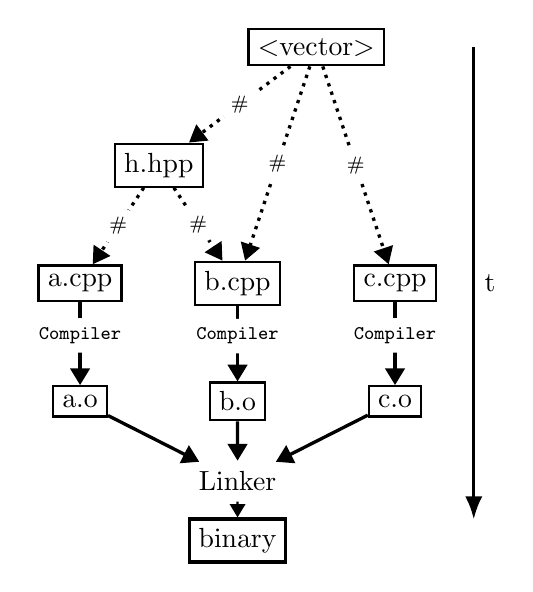
\begin{tikzpicture} [
            -Triangle,
            very thick
          ]
          \draw [-Latex](5,6) -- (5,0)  node [midway,right] {t};
          \path[thick]
            node (vec)  at(3,6)   [draw, rectangle] {\textless{}vector\textgreater{}}
            node (hpp)  at(1,4.5) [draw, rectangle] {h.hpp}
            node (acpp) at(0,3)   [draw, rectangle] {a.cpp}
            node (bcpp) at(2,3)   [draw, rectangle] {b.cpp}
            node (ccpp) at(4,3)   [draw, rectangle] {c.cpp}
            node (ao)   at(0,1.5) [draw, rectangle] {a.o}
            node (bo)   at(2,1.5) [draw, rectangle] {b.o}
            node (co)   at(4,1.5) [draw, rectangle] {c.o};

          \node[below= 0.5 cm of bo,fill=white,rounded rectangle] (link) {Linker};
          \node[below= 0.2 cm of link,rectangle,draw] (bin) {binary};

          \draw[very thick,dotted] (vec)  -- (hpp)  node [midway,fill=white,rounded rectangle] {\scriptsize \#};
          \draw[very thick,dotted] (vec)  -- (bcpp) node [midway,fill=white,rounded rectangle] {\scriptsize \#};
          \draw[very thick,dotted] (vec)  -- (ccpp) node [midway,fill=white,rounded rectangle] {\scriptsize \#};
          \draw[very thick,dotted] (hpp)  -- (acpp) node [midway,fill=white,rounded rectangle] {\scriptsize \#};
          \draw[very thick,dotted] (hpp)  -- (bcpp) node [midway,fill=white,rounded rectangle] {\scriptsize \#};
          \draw[very thick] (acpp) -- (ao)   node [pos=0.4,fill=white,rounded rectangle] {\scriptsize \texttt{Compiler}};
          \draw[very thick] (bcpp) -- (bo)   node [pos=0.4,fill=white,rounded rectangle] {\scriptsize \texttt{Compiler}};
          \draw[very thick] (ccpp) -- (co)   node [pos=0.4,fill=white,rounded rectangle] {\scriptsize \texttt{Compiler}};
          \draw[very thick] (ao)   -- (link);
          \draw[very thick] (bo)   -- (link);
          \draw[very thick] (co)   -- (link);
          \draw[thick] (link) -- (bin);

        \end{tikzpicture}
      \end{block}
    \end{column}
  \end{columns}
\end{frame}

\begin{frame}[fragile]
  \frametitlecpp[20]{Build system}
  \begin{columns}
    \begin{column}{.35\textwidth}
      \small
      \begin{block}{h.cpp}
        \begin{cppcode*}{gobble=6,linenos=false}
          export module foo;
          import <vector>;
          ...
        \end{cppcode*}
      \end{block}
      \begin{block}{a.cpp}
        \begin{cppcode*}{gobble=6,linenos=false}
          import foo;
          ...
        \end{cppcode*}
      \end{block}
      \begin{block}{b.cpp}
        \begin{cppcode*}{gobble=6,linenos=false}
          import <vector>;
          import foo;
          ...
        \end{cppcode*}
      \end{block}
      \begin{block}{c.cpp}
        \begin{cppcode*}{gobble=6,linenos=false}
          #include <vector>
          ...
        \end{cppcode*}
      \end{block}
    \end{column}
    \begin{column}{.6\textwidth}
      \begin{block}{New workflow}
        \center
        \resizebox{0.8\textwidth}{!}{%
        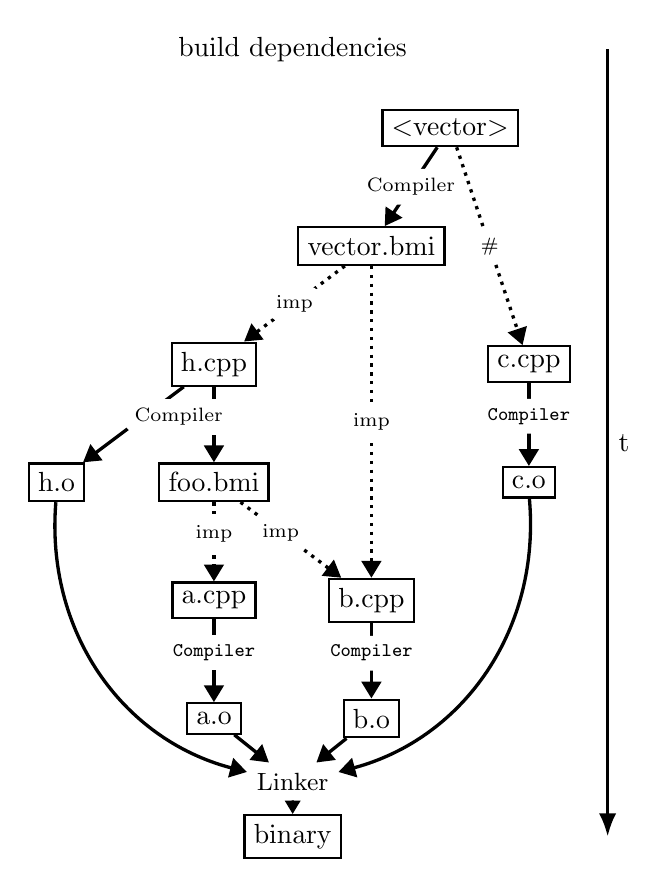
\begin{tikzpicture}[
              -Triangle,
              very thick
            ]
          \draw [-Latex](7,10) -- (7,0)  node [midway,right] {t};
          \draw[thick] node at(3, 10) [fill=white,rounded rectangle] {build dependencies};
          \path[thick]
          node (vec)    at(5,9)   [rectangle,draw] {\textless{}vector\textgreater{}}
          node (vecbmi) at(4,7.5) [rectangle,draw] {vector.bmi}
          node (hcpp)   at(2,6)   [rectangle,draw] {h.cpp}
          node (ho)     at(0,4.5) [rectangle,draw] {h.o}
          node (hbmi)   at(2,4.5) [rectangle,draw] {foo.bmi}
          node (acpp)   at(2,3)   [rectangle,draw] {a.cpp}
          node (bcpp)   at(4,3)   [rectangle,draw] {b.cpp}
          node (ccpp)   at(6,6)   [rectangle,draw] {c.cpp}
          node (ao)     at(2,1.5) [rectangle,draw] {a.o}
          node (bo)     at(4,1.5) [rectangle,draw] {b.o}
          node (co)     at(6,4.5) [rectangle,draw] {c.o}
          node (link)   at(3,0.7) [fill=white, rounded rectangle] {\small Linker}
          node (bin)    at(3,0)   [rectangle,draw] {binary};
          \draw[very thick,dotted] (vec) -- (ccpp) node [midway,fill=white,rounded rectangle] {\scriptsize \#};
          \draw[very thick] (vec) -- (vecbmi) node [midway,fill=white,rounded rectangle] {\scriptsize Compiler};
          \draw[very thick,dotted] (vecbmi) -- (hcpp) node [midway,fill=white,rounded rectangle] {\scriptsize imp};
          \draw[very thick] (hcpp) -- (ho) node [pos=0.4] (hoLeft) {};
          \draw[very thick] (hcpp) -- (hbmi) node [pos=0.4] (hoRight) {};
          \path (hoLeft) -- (hoRight) node[midway,fill=white,rounded rectangle] {\scriptsize Compiler};
          \draw[very thick,dotted] (vecbmi) -- (bcpp) node [midway,fill=white,rounded rectangle] {\scriptsize imp};
          \draw[very thick,dotted] (hbmi) -- (acpp) node [pos=0.4,fill=white,rounded rectangle] {\scriptsize imp};
          \draw[very thick,dotted] (hbmi) -- (bcpp) node [pos=0.4,fill=white,rounded rectangle] {\scriptsize imp};
          \draw[very thick] (acpp) -- (ao) node [pos=0.4,fill=white,rounded rectangle] {\scriptsize \texttt{Compiler}};
          \draw[very thick] (bcpp) -- (bo) node [pos=0.4,fill=white,rounded rectangle] {\scriptsize \texttt{Compiler}};
          \draw[very thick] (ccpp) -- (co) node [pos=0.4,fill=white,rounded rectangle] {\scriptsize \texttt{Compiler}};
          \draw[very thick] (ho) to [bend right=40] (link);
          \draw[very thick] (ao) -- (link);
          \draw[very thick] (bo) -- (link);
          \draw[very thick] (co) to [bend left=40] (link);
          \draw[thick] (link) -- (bin);
        \end{tikzpicture}
        }
      \end{block}
    \end{column}
  \end{columns}
\end{frame}

\begin{frame}[fragile]
    \frametitle{Build system}
    \begin{block}{New challenges}
      \begin{itemize}
        \item Resolving a module name to the file name building it
        \item Translation units no longer independent
        \begin{itemize}
          \item Extra tool needs to infer dependency graph before building
          \item This graph needs to be communicated to the build system
          \item We will likely need a \href{https://wg21.link/P1689}{standard dependency file format}
          \item Parallel and distributed builds need synchronization
        \end{itemize}
        \item Compilation of module translation units produces binary module interface (BMI) and object file
        \begin{itemize}
          \item BMIs need to be maintained/shared between multiple compiler instances
        \end{itemize}
        \item Tools beside the compiler need to build/read binary module interface (static analysis, auto completion, etc.)
        \item The C++ standard specifies very little on how this works
        \begin{itemize}
          \item We may experience large implementation divergence
        \end{itemize}
      \end{itemize}
    \end{block}
\end{frame}

\begin{frame}[fragile]
    \frametitlecpp[20]{Build system}
    \begin{block}{Status}
      \begin{itemize}
        \item build2 supports everything g++ does
        \item MSBuild figures out dependencies and build order automatically (Windows/Visual Studio only)
        \item \cppinline{g++ a.cpp b.cpp ...} ``just works'', must be one line though
        \item GCC uses a \href{https://wg21.link/P1184}{module mapper} to resolve imports, which specifies a protocol and uses a central server for module maintenance
        \item \href{https://wg21.link/p1602}{Experimental extensions to GNU make} exist to grow dependency graph on the fly while modules are discovered
        \item No support in cmake (3.23) yet
      \end{itemize}
    \end{block}
\end{frame}

\begin{frame}[fragile]
    \frametitlecpp[20]{Building modules (g++)}
    \begin{block}{Case study: g++}
      \begin{itemize}
        \item By default, g++ caches compiled module interfaces (CMI, i.e.\ BMI) in subdirectory \texttt{./gcm.cache}
        \item Each module needs to be built before it can be imported
        \begin{itemize}
          \item {\footnotesize \cppinline{g++ -std=c++20 -fmodules-ts -c ratio.cpp -o ratio.o}}
          \item Generates \texttt{ratio.o} and \texttt{./gcm.cache/ratio.gcm} (CMI)
        \end{itemize}
        \item Each header unit needs to be built before it can be imported
        \begin{itemize}
          \item {\footnotesize \cppinline{g++ -std=c++20 -fmodules-ts -x c++-system-header vector}}
          \item Generates e.g.\ \texttt{./gcm.cache/usr/include/c++/11/vector.gcm} (CMI)
          \item {\footnotesize \cppinline{g++ -std=c++20 -fmodules-ts -x c++-header ratio.h}}
          \item Generates e.g.\ \texttt{./gcm.cache/,/ratio.h.gcm} (CMI)
        \end{itemize}
      \end{itemize}
    \end{block}
\end{frame}

\begin{frame}[fragile]
    \frametitlecpp[20]{Modules}
    \begin{exampleblock}{Guidance for today}
      \begin{itemize}
        \item Start writing importable headers (no macro dependencies)
        \begin{itemize}
          \item This allows dual use: \cppinline{#include} before \cpp20 and \cppinline{import} with \cpp20
        \end{itemize}
        \item Watch progress on module support in your build system
      \end{itemize}
    \end{exampleblock}
    \begin{exampleblock}{Guidance for tomorrow}
      \begin{itemize}
        \item Start importing headers when \cpp20 is available
        \item Start writing modules when all users of your code have \cpp20
        \item Start using \cppinline{import std;} when \cpp23 is available
      \end{itemize}
    \end{exampleblock}
\end{frame}

\begin{frame}[fragile]
    \frametitlecpp[20]{Modules}
    \begin{block}{Resources}
      \begin{itemize}
      \item \href{https://www.youtube.com/watch?v=szHV6RdQdg8}{Practical C++ Modules - Boris Kolpackov - CppCon 2019}
      \item \href{https://www.youtube.com/watch?v=nP8QcvPpGeM}{A (Short) Tour of C++ Modules - Daniela Engert - CppCon 2021} (very technical)
      \item Understanding C++ Modules: \href{https://vector-of-bool.github.io/2019/03/10/modules-1.html}{Part1}, \href{https://vector-of-bool.github.io/2019/03/31/modules-2.html}{Part2} and \href{https://vector-of-bool.github.io/2019/10/07/modules-3.html}{Part3}.
      \end{itemize}
    \end{block}
\end{frame}

\begin{frame}[fragile]
  \frametitlecpp[20]{Modules}
  \begin{exercise}{Modules}
    \begin{itemize}
      \item go to \texttt{exercises/modules}
      \item convert the \texttt{Complex.hpp} header into a module named \texttt{math}
    \end{itemize}
  \end{exercise}
  \begin{exercise}{Header units}
    \begin{itemize}
      \item go to \texttt{exercises/header\_units}
      \item convert all \cppinline{#include}s into header unit \cppinline{import}s
    \end{itemize}
  \end{exercise}
\end{frame}

  \subsection{Coroutines}

\begin{frame}[fragile]
  \frametitlecpp[20]{Why do we need coroutines?}
  \begin{block}{The generator use case (one of several)}
    In python one can write
    {\scriptsize
      \begin{pythoncode*}{gobble=2}
        for i in range(0, 10):
          print(i)
      \end{pythoncode*}
    }
    What about it in \cpp?
    {\scriptsize
      \begin{cppcode*}{gobble=2, firstnumber=3}
        someType range(int first, int last) { ... }
        for (auto i : range(0, 10)) {
          std::cout << i << "\n";
        }
      \end{cppcode*}
    }
    How can we implement range?
  \end{block}
  \begin{exampleblock}{Requirements}
    \begin{itemize}
    \item \mintinline{cpp}{someType} needs to be some iterable type
    \item \mintinline{cpp}{range} should execute lazily, only creating values on demand
    \item meaning \mintinline{cpp}{range} should be suspended and resumed
    \end{itemize}
    That's what coroutines are for!
  \end{exampleblock}
\end{frame}

\begin{frame}[fragile]
  \frametitlecpp[20]{What \cpp20 allows}
  \begin{exampleblock}{Interesting part of the implementation (see \href{https://en.cppreference.com/w/cpp/coroutine/coroutine\_handle\#Example}{\color{blue!50!white}cppreference})}
    {\scriptsize
      \begin{cppcode*}{gobble=2}
        template<std::integral T>
        Generator<T> range(T first, const T last) {
          while (first < last) {
            co_yield first++;
          }
        }
        for (const char i : range(65, 91)) {
          std::cout << i << ' ';
        }
        std::cout << '\n';
      \end{cppcode*}
    }
  \end{exampleblock}
  \begin{alertblock}{The bad news}
    \begin{itemize}
    \item class \mintinline{cpp}{Generator} is not provided by the STL
    \item and is ~80 lines of boiler plate code...
    \item may be sorted out in \cpp23
    \item in the meantime, we'll have to dive into some details!
    \end{itemize}
  \end{alertblock}
\end{frame}

\begin{frame}
  \frametitlecpp[20]{A few concepts first}
  \begin{block}{Definition of a coroutine}
    \begin{itemize}
    \item a function which can be suspended and resumed
      \begin{itemize}
      \item potentially by another caller (even on a different thread)
      \end{itemize}
    \item practically a function using one of:
      \begin{description}
      \item[\mintinline{cpp}{co_await}] suspends execution
      \item[\mintinline{cpp}{co_yield}] suspends execution and returns a value
      \item[\mintinline{cpp}{co_return}] completes execution
      \end{description}
    \end{itemize}
  \end{block}
  \begin{alertblock}{Implications}
    \begin{itemize}
    \item on suspension, the state of the function needs to be preserved
    \item the suspended function becomes pure data on the heap
    \item access to this data is given via the returned value
      \begin{itemize}
      \item so the returned type must follow some convention
      \item it needs to contain a \mintinline{cpp}{struct promise_type}
      \end{itemize}
    \end{itemize}
  \end{alertblock}
\end{frame}

\begin{frame}[fragile]
  \frametitlecpp[20]{Minimal code}
  \begin{block}{Definition of an empty coroutine}
    {\scriptsize
      \begin{cppcode*}{gobble=2, firstnumber=3}
        #include <coroutine>
        struct Task {
          struct promise_type {
            Task get_return_object() { return {}; }
            std::suspend_never initial_suspend() { return {}; }
            std::suspend_never final_suspend() noexcept { return {}; }
            void return_void() {}
            void unhandled_exception() { throw; }
          };
        };
        Task myCoroutine() { co_return; }
        int main() { Task x = myCoroutine(); }
      \end{cppcode*}
    }
  \end{block}
  \begin{exampleblock}{\texttt{promise\_type} interface}
    \begin{description}[\small \mintinline{cpp}{initial/final_suspend}]
      \setlength{\itemsep}{0pt}
    \item[\small \mintinline{cpp}{get_return_object}] builds a Task from the given promise
    \item[\small \mintinline{cpp}{initial/final_suspend}] called before/after coroutine starts/ends
    \item[\small \mintinline{cpp}{unhandled_exception}] called in case of exception in coroutine
    \item[\small \mintinline{cpp}{return_void/value}] returns final value of the coroutine
    \end{description}
  \end{exampleblock}
\end{frame}

\begin{frame}[fragile]
  \frametitlecpp[20]{Minimal sequence of events (nothing suspended)}
  \begin{block}{Compiler generated set of calls when calling \mintinline{cpp}{myCoroutine}}
    \center
    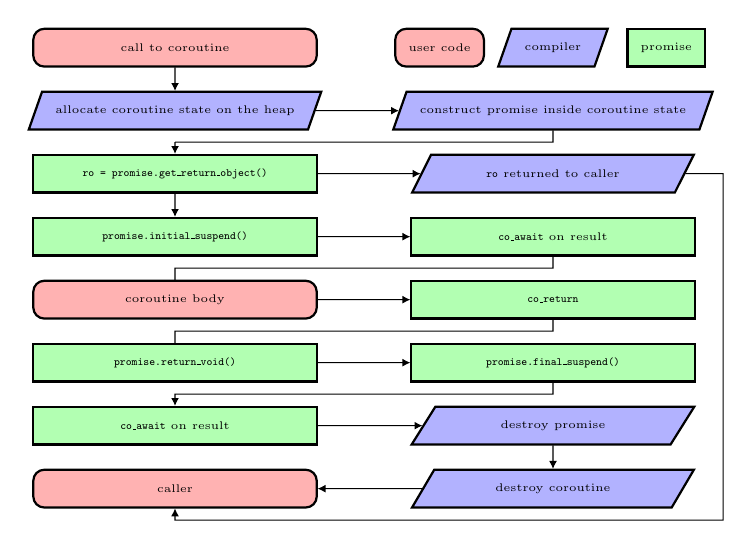
\begin{tikzpicture}[->, node distance=.75cm, font=\tiny, scale=0.8, every node/.style={scale=0.8},xscale=6,-{Latex[length=1mm,width=1mm]}]
      \tikzstyle{call}=[rectangle,draw=black,thick,inner sep=6pt,rounded corners,minimum width=4.5cm,minimum height=.6cm,fill=red!30]
      \tikzstyle{comp}=[trapezium,trapezium left angle=70,trapezium right angle=110,draw=black,thick,inner sep=6pt,trapezium stretches=true,minimum width=4.5cm,minimum height=.6cm,fill=blue!30]
      \tikzstyle{box}=[rectangle,draw=black,thick,inner sep=6pt,minimum width=4.5cm,minimum height=.6cm,fill=green!30]
      \node[call] at (0, 0) (initCall) {call to coroutine};
      \node[comp] at (0,-1) (allocState) {allocate coroutine state on the heap};
      \node[comp] at (1,-1) (construct) {construct promise inside coroutine state};
      \node[box]  at (0,-2) (getReturn) {\texttt{ro = promise.get\_return\_object()}};
      \node[comp] at (1,-2) (localVar) {\texttt{ro} returned to caller};
      \node[box]  at (0,-3) (initSuspend) {\texttt{promise.initial\_suspend()}};
      \node[box] at (1,-3) (initWait) {\texttt{co\_await} on result};
      \node[call] at (0,-4) (body) {coroutine body};
      \node[box]  at (1,-4) (coreturn) {\texttt{co\_return}};
      \node[box] at (1,-5) (finalSuspend) {\texttt{promise.final\_suspend()}};
      \node[box]  at (0,-6) (finalWait) {\texttt{co\_await} on result};
      \node[box]  at (0,-5) (return) {\texttt{promise.return\_void()}};
      \node[comp]  at (1,-6) (destroyP) {destroy promise};
      \node[call] at (0,-7) (caller) {caller};
      \node[comp]  at (1,-7) (destroyC) {destroy coroutine};
      \draw (initCall)      edge (allocState)
            (allocState)    edge (construct)
            (construct)     --   +(0,-.5) -| +(-1,-0.5) edge (getReturn)
            (getReturn)     edge (localVar)
            (localVar.east) --   +(0.1,0) |- (1,-7.5) -| (caller);
      \draw (getReturn)    edge (initSuspend)
            (initSuspend)  edge (initWait)
            (initWait)     -- +(0,-.5) -| (body)
            (body)         edge (coreturn)
            (coreturn)     -- +(0,-.5) -| (return)
            (return)       edge (finalSuspend)
            (finalSuspend) -- +(0,-.5) -| (finalWait)
            (finalWait)    edge (destroyP)
            (destroyP)     edge (destroyC)
            (destroyC)     edge (caller);
      \node[call,minimum width=1cm] at (.7, 0) {user code};
      \node[comp,minimum width=1cm] at (1, 0) {compiler};
      \node[box, minimum width=1cm] at (1.3, 0) {promise};
    \end{tikzpicture}
  \end{block}
\end{frame}

\begin{frame}[fragile]
  \frametitlecpp[20]{Suspending a coroutine}
  \begin{block}{Main way to suspend a coroutine: \mintinline{cpp}{co_wait}}
    \begin{itemize}
    \item it's an expression taking an ``awaitable''/ ``awaiter''
      \begin{itemize}
      \item we'll ignore the distinction for now
      \end{itemize}
    \item 2 trivial awaiters are provided by the STL: \mintinline{cpp}{std::suspend_always} and \mintinline{cpp}{std::suspend_never}
    \item obviously only the first one will trigger a suspension
      \begin{itemize}
      \item note the other one is used in the minimal code
      \end{itemize}
    \item more details on awaiters later
    \end{itemize}
  \end{block}
  \begin{exampleblock}{Code}
    {\scriptsize
      \begin{cppcode*}{gobble=4}
        Task myCoroutine() {
          std::cout << "Step 1 of coroutine\n";
          co_await std::suspend_always{};
          std::cout << "Step 2 of coroutine\n";
          co_await std::suspend_always{};
          std::cout << "final step\n";
        }
      \end{cppcode*}
    }
  \end{exampleblock}
\end{frame}

\begin{frame}[fragile]
  \frametitlecpp[20]{Resuming a coroutine}
  \begin{block}{Principles}
    \begin{itemize}
    \item one needs to call \mintinline{cpp}{resume()} on the \mintinline{cpp}{coroutine_handle}
    \item BUT user code has no such handle
      \begin{itemize}
      \item only the coroutine return object (here a \mintinline{cpp}{Task} instance)
      \end{itemize}
    \item so one has to amend the Task class
      \begin{itemize}
      \item and the \mintinline{cpp}{promise_type} as it's building the \mintinline{cpp}{Task} instance
      \end{itemize}
    \end{itemize}
  \end{block}
  \begin{exampleblock}{Code}
    {\scriptsize
      \begin{cppcode*}{gobble=4}
        struct Task {
          struct promise_type {
            Task get_return_object() {
              // build Task with the coroutine handle
              return {std::coroutine_handle<promise_type>::from_promise(*this)};
            }
            ... // rest is unchanged
          };
          std::coroutine_handle<promise_type> h_;
          void resume() { h_.resume(); }
        };
      \end{cppcode*}
    }
  \end{exampleblock}
\end{frame}

\begin{frame}[fragile]
  \frametitlecpp[20]{Resuming a coroutine}
  \scriptsize
  \begin{block}{User code - \href{https://godbolt.org/z/qx46Pa4v3}{\color{blue!50}godbolt}}
    \begin{cppcode*}{gobble=2}
      Task myCoroutine() {
        std::cout << "Step 1 of coroutine\n";
        co_await std::suspend_always{};
        std::cout << "Step 2 of coroutine\n";
        co_await std::suspend_always{};
        std::cout << "final step\n";
      }
      int main() {
        auto c = myCoroutine(); // Step 1 runs
        std::cout << "In main, between Step 1 and 2\n";
        c.resume();             // Step 2 runs
        std::cout << "In main, between Step 2 and final step\n";
        c.resume();             // final Step runs
        // c.resume(); // would segfault!
      }
    \end{cppcode*}
  \end{block}
  \begin{block}{}
    \begin{minted}[gobble=4]{text}
      Step 1 of coroutine
      In main, between Step 1 and 2
      Step 2 of coroutine
      In main, between Step 2 and final step
      final step
    \end{minted}
  \end{block}
\end{frame}

\begin{frame}[fragile]
  \frametitlecpp[20]{A few more details}
  \begin{block}{About suspension of coroutines}
    \begin{itemize}
    \item \mintinline{cpp}{initial/final_suspend} methods allow to suspend a coroutine at the very start/end (after \mintinline{cpp}{co_return})
    \item a suspended coroutine is not deallocated
      \begin{itemize}
      \item i.e.\ its state will stay on the heap
      \item so you can leak coroutines!
      \end{itemize}
    \item one can directly call \mintinline{cpp}{coroutine_handle::destroy} if the execution of a suspended coroutine should be aborted
      \begin{itemize}
      \item which requires another piece of code in \mintinline{cpp}{Task}, e.g.
        {\scriptsize
          \begin{cppcode*}{gobble=8,linenos=false}
            ~Task() { if (h_) h_.destroy(); }
          \end{cppcode*}
        }
      \end{itemize}
    \item the \mintinline{cpp}{Task} class should be move only
     \end{itemize}
  \end{block}
  \begin{alertblock}{We need standard \mintinline{cpp}{Task} classes in the STL!}
    \begin{itemize}
    \item \mintinline{cpp}{std::generator} may come in \cpp23
     \end{itemize}
    \end{alertblock}
\end{frame}

\begin{frame}[fragile]
  \frametitlecpp[20]{\texttt{co\_yield} - returning a value upon suspension}
  \begin{block}{What \texttt{co\_yield} really is}
    \begin{itemize}
    \item an expression like \mintinline{cpp}{co_await}
    \item a shortcut for \mintinline{cpp}{co_await promise.yield_value(expr)}
    \item and we have to provide the \mintinline{cpp}{yield_value} method of \mintinline{cpp}{promise_type} and the \mintinline{cpp}{Task} accessor
    \end{itemize}
  \end{block}
  \begin{exampleblock}{Typical code}
    {\scriptsize
      \begin{cppcode*}{gobble=4}
        template<typename T> struct Task {
          struct promise_type {
            T value_;
            std::suspend_always yield_value(T&& from) {
              value_ = std::forward<T>(from); // caching the result
              return {};
            }
            ... // rest is unchanged
          };
          T getValue() { return h_.promise().value_; } // accessor for user code
        };
      \end{cppcode*}
    }
  \end{exampleblock}
\end{frame}

\begin{frame}[fragile]
  \frametitlecpp[20]{\texttt{co\_yield} - generator behavior}
  \begin{block}{Generator behavior - more boiler plate code}
    {\scriptsize
      \begin{cppcode*}{gobble=4}
        template<typename T>
        struct Task {
          struct iterator {
            std::coroutine_handle<promise_type> handle;
            auto &operator++() {
              handle.resume();
              if (handle.done()) { handle = nullptr; } // == end iterator
              return *this;
            }
            auto operator++(int) { ++*this; }
            T const& operator*() const { return handle.promise().value_; }
            ...
          };
          iterator begin() { resume(); return {h_}; }
          iterator end() { return {nullptr}; }
          ... // plus error handling is missing
        };
      \end{cppcode*}
    }
  \end{block}
\end{frame}

\begin{frame}[fragile]
  \frametitlecpp[20]{\texttt{co\_yield} - final usage}
  \begin{exampleblock}{Finally, we can use the generator nicely - \href{https://godbolt.org/z/6bbrYrss5}{\color{blue!50}godbolt}}
    {\scriptsize
      \begin{cppcode*}{gobble=4}
        Task range(int first, int last) {
          while (first != last) {
            co_yield first++;
          }
        }
        for (int i : range(0, 10)) {
          std::cout << i << "";
        } // 1 2 3 4 5 6 7 8 9
      \end{cppcode*}
    }
  \end{exampleblock}
  \pause
  \begin{alertblock}{Wait a minute: 0 is missing in the output!}
    \begin{itemize}
    \item resume called in \mintinline{cpp}{operator++} before 0 is printed
    \item we should pause in \mintinline{cpp}{initial_suspend}
    \end{itemize}
     {\scriptsize
      \begin{cppcode*}{gobble=4,firstnumber=10}
        struct Task {
          struct promise_type {
            ...
            std::suspend_always initial_suspend() { return {}; }
            ...
          }
        };
      \end{cppcode*}
    }
  \end{alertblock}
\end{frame}

\begin{frame}[fragile]
  \frametitlecpp[20]{Lazyness allows for infinite ranges}
  \begin{block}{Generators do not need to be finite - \href{https://godbolt.org/z/MP6qdGWYe}{\color{blue!50}godbolt}}
    \begin{cppcode*}{gobble=2}
      Task range(int first) {
        while (true) {
          co_yield first++;
        }
      }
      for (int i : range(0) | std::views::take(10)) {
        std::cout << i << "\n";
      }
    \end{cppcode*}
  \end{block}
\end{frame}

\begin{frame}[fragile]
  \frametitlecpp[20]{Real life example}
  \begin{block}{A Fibonacci generator - \href{https://godbolt.org/z/3Pev1M8se}{\color{blue!50}godbolt}, from \href{https://en.cppreference.com/w/cpp/language/coroutines}{\color{blue!50}cppreference}}
    \scriptsize
     \begin{cppcode*}{gobble=2}
       Task<long long int> fibonacci(unsigned n) {
         if (n==0) co_return;
         co_yield 0;
         if (n==1) co_return;
         co_yield 1;
         if (n==2) co_return;
         uint64_t a=0;
         uint64_t b=1;
         for (unsigned i = 2; i < n; i++) {
           uint64_t s=a+b;
           co_yield s;
           a=b;
           b=s;
         }
       }

       int main() {
         for (int i : fibonacci(10)) {
           std::cout << i << "\n";
         }
       }
    \end{cppcode*}
  \end{block}
\end{frame}

\begin{frame}
  \frametitlecpp[20]{Coming back to awaitables/awaiters}
  \begin{block}{awaitables vs awaiters}
    \begin{itemize}
    \item awaitable is the type required by \mintinline{cpp}{co_await}/\mintinline{cpp}{co_yield}
      \begin{itemize}
      \item or the expression given has to be convertible to awaitable
      \item alternatively the \mintinline{cpp}{promise_type} can have an \mintinline{cpp}{await_transform} method returning an awaitable
      \end{itemize}
    \item an awaiter is retrieved from the awaitable by the compiler
      \begin{itemize}
      \item either by calling operator \mintinline{cpp}{co_wait} on it
      \item or via direct conversion if no such operator exists
      \end{itemize}
    \item an awaiter has 3 main methods
      \begin{itemize}
      \item \mintinline{cpp}{await_ready}, \mintinline{cpp}{await_suspend} \mintinline{cpp}{and await_resume}
      \end{itemize}
    \end{itemize}
  \end{block}
\end{frame}

\begin{frame}[fragile]
  \frametitlecpp[20]{How awaiters work}
  \begin{block}{Compiler generated set of calls}
    \center
    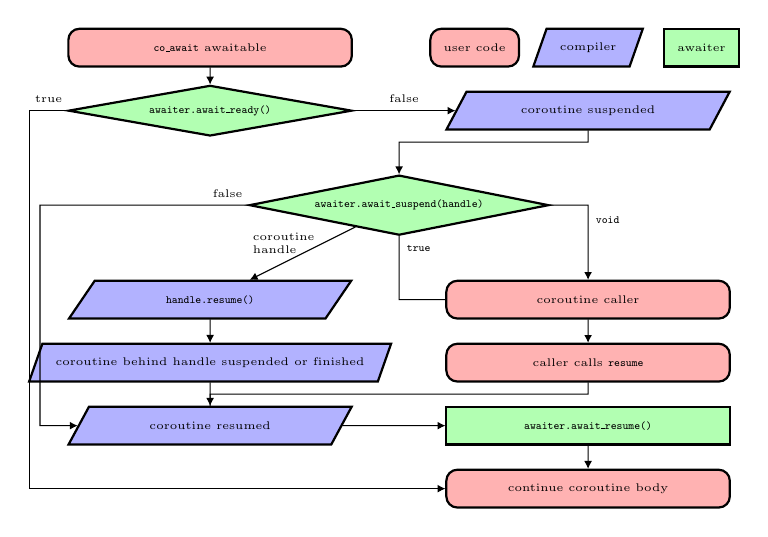
\begin{tikzpicture}[->, node distance=.75cm, font=\tiny, scale=0.8, every node/.style={scale=0.8},xscale=6,-{Latex[length=1mm,width=1mm]}]
      \tikzstyle{call}=[rectangle,draw=black,thick,inner sep=6pt,rounded corners,minimum width=4.5cm,minimum height=.6cm,fill=red!30]
      \tikzstyle{comp}=[trapezium,trapezium left angle=70,trapezium right angle=110,draw=black,thick,inner sep=6pt,trapezium stretches=true,minimum width=4.5cm,minimum height=.6cm,fill=blue!30]
      \tikzstyle{box}=[rectangle,draw=black,thick,inner sep=6pt,minimum width=4.5cm,minimum height=.6cm,fill=green!30]
      \tikzstyle{choice}=[diamond,draw=black,thick,inner sep=3pt,minimum width=4.5cm,minimum height=.6cm,fill=green!30,aspect=5]
      \node[call]   at (0, 0) (co_await) {\texttt{co\_await} awaitable};
      \node[choice] at (0,-1) (await_ready) {\texttt{awaiter.await\_ready()}};
      \node[comp]   at (1,-1) (suspend) {coroutine suspended};
      \node[choice] at (.5,-2.5) (await_suspend) {\texttt{awaiter.await\_suspend(handle)}};
      \node[comp]   at (0,-4) (handleresume) {\texttt{handle.resume()}};
      \node[call]   at (1,-4) (caller) {coroutine caller};
      \node[comp]   at (0,-5) (corofin) {coroutine behind handle suspended or finished};
      \node[call]   at (1,-5) (callresume) {caller calls \texttt{resume}};
      \node[comp]   at (0,-6) (resumed) {coroutine resumed};
      \node[box]    at (1,-6) (await_resume) {\texttt{awaiter.await\_resume()}};
      \node[call]   at (1,-7) (body) {continue coroutine body};
      \draw (co_await)      edge (await_ready)
            (await_ready)   edge node[above] {false}  (suspend)
            (await_ready.west) -- node[above] {true} +(-0.1,0) |- (body);
      \draw (suspend)       -- +(0,-.5)  -|   (await_suspend);
      \draw (await_suspend) -- node[above,pos=.1] {false} +(-.95,0) |- (resumed);
      \draw (await_suspend) edge node[text width=1cm,left,pos=.3] {coroutine handle} (handleresume)
            (handleresume)  edge (corofin)
            (corofin)       edge (resumed)
            (await_suspend) |- node[right,pos=0.1] {\texttt{true}}  (caller)
            (caller)        edge (callresume)
            (callresume)    --   +(0,-.5) -| (resumed)
            (await_suspend) -|  node[right,pos=0.6] {\texttt{void}}  (caller)
            (resumed)       edge (await_resume)
            (await_resume)       edge (body);
      \node[call,minimum width=1cm] at (.7, 0) {user code};
      \node[comp,minimum width=1cm] at (1, 0) {compiler};
      \node[box, minimum width=1cm] at (1.3, 0) {awaiter};
    \end{tikzpicture}
  \end{block}
\end{frame}

\begin{frame}[fragile]
  \frametitlecpp[20]{\texttt{awaiter} example}
  \begin{block}{Switch to new thread - \href{https://godbolt.org/z/K7svE4P7s}{\color{blue!50}godbolt}, from \href{https://en.cppreference.com/w/cpp/language/coroutines}{\color{blue!50}cppreference}}
    \scriptsize
    \begin{cppcode*}{gobble=2}
      auto switch_to_new_thread(std::jthread& out) {
        struct awaiter {
          std::jthread* th;
          bool await_ready() { return false; }
          void await_suspend(std::coroutine_handle<> h) {
            *th = std::jthread([h] { h.resume(); });
            std::cout << "New thread ID: " << th->get_id() << '\n';
          }
          void await_resume() {}
        };
        return awaiter{&out};
      }
      Task<int> resuming_on_new_thread(std::jthread& out) {
        std::cout << "Started on " << std::this_thread::get_id() << '\n';
        co_await switch_to_new_thread(out);
        std::cout << "Resumed on " << std::this_thread::get_id() << std::endl;
      }
      int main() {
        std::jthread out;
        resuming_on_new_thread(out);
      }
     \end{cppcode*}
  \end{block}
  \pause
  \vspace{-2.1cm}
  \begin{columns}
    \begin{column}{.45\textwidth}
    \end{column}
    \begin{column}{.55\textwidth}
      \setlength{\textwidth}{5.4cm}
      \raggedright
      \begin{exampleblock}{Output}
        \scriptsize
        \begin{minted}[gobble=9]{text}
          Started on thread: 140144191063872
          New thread ID: 140144191059712
          Resumed on thread: 140144191059712
        \end{minted}
      \end{exampleblock}
    \end{column}
  \end{columns}
\end{frame}

\begin{frame}[fragile]
  \frametitlecpp[20]{Summary on coroutines}
  \begin{exampleblock}{Coroutines are usable in \cpp20}
    \begin{itemize}
    \item allow to have nice generators
    \item also very useful for async/IO code
      \begin{itemize}
      \item another big use case which we did not touch
      \end{itemize}
    \end{itemize}
  \end{exampleblock}
  \begin{alertblock}{But library support is poor for now}
    \begin{itemize}
    \item standard Task/Generator classes are not provided
    \item leading to \emph{lots of boiler plate code} for the end user
    \item \mintinline{cpp}{std::generator} is part of \cpp23's draft
    \item in the meantime, libraries exist, e.g. \href{https://github.com/lewissbaker/cppcoro}{CppCoro}
    \end{itemize}
  \end{alertblock}
\end{frame}

\end{advanced}

\section[Tool]{Useful tools}
\subsection[edit]{\cpp editor}

\begin{frame}[fragile]
  \frametitle{\cpp editors and IDEs}
  \begin{block}{Can dramatically improve your efficiency by}
    \begin{itemize}
      \item Coloring the code for you to ``see'' the structure
      \item Helping with indenting and formatting properly
      \item Allowing you to easily navigate in the source tree
      \item Helping with compilation/debugging, profiling, static analysis
      \item Showing you errors and suggestions while typing
    \end{itemize}
  \end{block}
  \begin{block}{}
    \begin{description}
    \item[\href{http://www.microsoft.com/}{\beamergotobutton{Visual Studio}}]
      Heavy, fully fledged IDE for Windows
    \item[\href{https://code.visualstudio.com/}{\beamergotobutton{Visual Studio Code}}]
      Editor, open source, portable, many plugins
    \item[\href{https://www.eclipse.org/}{\beamergotobutton{Eclipse}}]
      IDE, open source, portable
    \item[\href{http://www.gnu.org/software/emacs/}{\beamergotobutton{Emacs}} \href{https://www.vim.org/}{\beamergotobutton{Vim}}]
      Editors for experts, extremely powerful. \\
      They are to IDEs what latex is to PowerPoint
    \item[CLion, Code::Blocks, Atom, NetBeans, Sublime Text, ...]
    \end{description}
    Choosing one is mostly a matter of taste
  \end{block}
\end{frame}

\subsection[VCS]{Version control}

\begin{frame}[fragile]
  \frametitle{Version control}
  \begin{alertblock}{Please use one!}
    \begin{itemize}
    \item Even locally
    \item Even on a single file
    \item Even if you are the only committer
    \end{itemize}
    It will soon save your day
  \end{alertblock}
  \begin{block}{A few tools}
    \begin{description}
    \item[\href{http://git-scm.com/}{\beamergotobutton{git}}]
      THE mainstream choice. Fast, light, easy to use
    \item[\href{http://mercurial.selenic.com/}{\beamergotobutton{mercurial}}]
      The alternative to git
    \item[\href{http://bazaar.canonical.com/en/}{\beamergotobutton{Bazaar}}]
      Another alternative
    \item[\href{https://subversion.apache.org/}{\beamergotobutton{Subversion}}]
      Historical, not distributed - don't use
    \item[\href{https://cvs.nongnu.org/}{\beamergotobutton{CVS}}]
      Archeological, not distributed - don't use
    \end{description}
  \end{block}
\end{frame}

\begin{frame}[fragile]
  \frametitle{Git crash course}
  \begin{minted}[gobble=4]{shell-session}
    $ git init myProject
    Initialized empty Git repository in myProject/.git/

    $ vim file.cpp; vim file2.cpp
    $ git add file.cpp file2.cpp
    $ git commit -m "Committing first 2 files"
    [master (root-commit) c481716] Committing first 2 files
    ...

    $ git log --oneline
    d725f2e Better STL test
    f24a6ce Reworked examples + added stl one
    bb54d15 implemented template part
    ...

    $ git diff f24a6ce bb54d15
  \end{minted}
\end{frame}

\subsection[format]{Code formatting}

\begin{frame}[fragile]
\frametitle{clang-format}
\begin{block}{.clang-format}
	\begin{itemize}
		\item File describing your formatting preferences
		\item Should be checked-in at the repository root (project wide)
		\item \mintinline{bash}{clang-format -style=LLVM -dump-config >} \\
		  \mintinline{bash}{.clang-format}
		\item Adapt style options with help from: \url{https://clang.llvm.org/docs/ClangFormatStyleOptions.html}
	\end{itemize}
\end{block}
\begin{block}{Run clang-format}
	\begin{itemize}
		\item \mintinline{bash}{clang-format --style=LLVM -i <file.cpp>}
		\item \mintinline{bash}{clang-format -i <file.cpp>} (looks for .clang-format file)
		\item \mintinline{bash}{git clang-format} (formats local changes)
		\item \mintinline{bash}{git clang-format <ref>} (formats changes since git \textless{}ref\textgreater{})
		\item Some editors/IDEs find a .clang-format file and adapt
	\end{itemize}
\end{block}
\end{frame}

\begin{frame}[fragile]
\frametitle{clang-format}
\begin{exercise}{clang-format}
	\begin{itemize}
		\item Go to any example
		\item Format code with: \mintinline{bash}{clang-format --style=GNU -i <file.cpp>}
		\item Inspect changes, try \mintinline{bash}{git diff .}
		\item Revert changes using \mintinline{bash}{git checkout -- <file.cpp>} or \mintinline{bash}{git checkout .}
		\item Go to code directory and create a .clang-format file \\
		  \mintinline{bash}{clang-format -style=LLVM -dump-config >} \\
		  \mintinline{bash}{.clang-format}
		\item Run \mintinline{bash}{clang-format -i <any_exercise>/*.cpp}
		\item Revert changes using \mintinline{bash}{git checkout <any_exercise>}
	\end{itemize}
\end{exercise}
\end{frame}

\subsection[gcc]{The Compiling Chain}

\begin{frame}[fragile]
  \frametitlecpp[17]{The compiling chain}
  \center
  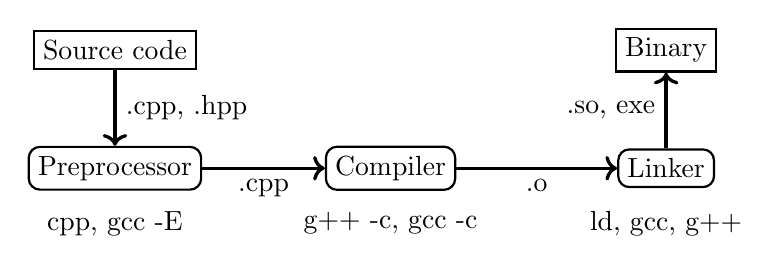
\begin{tikzpicture}
    \draw[thick] node (code) at(0,0) [rectangle,draw] {Source code}
                 node (cpp) at(0, -1.5cm) [rectangle,rounded corners,draw] {Preprocessor}
                 node (gcc) at(3.5cm,-1.5cm) [rectangle,rounded corners,draw] {Compiler}
                 node (ld) at(7cm,-1.5cm) [rectangle,rounded corners,draw] {Linker}
                 node (bin) at(7cm,0) [rectangle,draw] {Binary}
                 node at(0, -2.2cm) {cpp, gcc -E}
                 node at(3.5cm, -2.2cm) {g++ -c, gcc -c}
                 node at(7cm, -2.2cm) {ld, gcc, g++};
    \draw[very thick,->] (code) -- (cpp) node [midway,right] {.cpp, .hpp};
    \draw[very thick,->] (cpp) -- (gcc) node [midway,below] {.cpp};
    \draw[very thick,->] (gcc) -- (ld) node [midway,below] {.o};
    \draw[very thick,->] (ld) -- (bin) node [midway,left] {.so, exe};
  \end{tikzpicture}
  \begin{block}{The steps}
    \begin{description}
    \item[cpp]
        the preprocessor \\
        handles the \# directives (macros, includes) \\
        creates ``complete'' source code (ie. translation unit)
    \item[g++]
        the compiler \\
        creates machine code from \cpp code
    \item[ld]
        the linker \\
        links several binary files into libraries and executables
    \end{description}
  \end{block}
\end{frame}

\begin{frame}[fragile]
  \frametitle{Compilers}
  \begin{block}{Available tools}
    \begin{description}
    \item[\href{http://gcc.gnu.org/}{\beamergotobutton{gcc}}]
        the most common and most used\\
        free and open source
    \item[\href{http://clang.llvm.org/}{\beamergotobutton{clang}}]
        drop-in replacement of gcc \\
        slightly better error reporting \\
        free and open source, based on LLVM
    \item[\href{https://www.intel.com/content/www/us/en/developer/tools/oneapi/dpc-compiler.html\#gs.dyllp0}{\beamergotobutton{icc} \beamergotobutton{icx}}]
        Intel's compilers, proprietary but now free \\
        optimized for Intel hardware \\
        icc being replaced by icx, based on LLVM
    \item[\href{https://visualstudio.microsoft.com/}{\beamergotobutton{Visual \cpp / MSVC}}]
      Microsoft's C++ compiler on Windows
    \end{description}
  \end{block}
  \begin{alertblock}{My preferred choice today}
    \begin{itemize}
      \item \alert{gcc} as the de facto standard in HEP
      \item \hspace{0pt}\alert{clang} in parallel to catch more bugs
    \end{itemize}
  \end{alertblock}
\end{frame}

\begin{frame}[fragile]
  \frametitle{Useful compiler options (gcc/clang)}
  \begin{block}{Get more warnings}
    \begin{description}
      \item[-Wall -Wextra] get all warnings
      \item[-Werror] force yourself to look at warnings
    \end{description}
  \end{block}
  \begin{block}{Optimization}
    \begin{description}
      \item[-g] add debug symbols
      \item[-Ox] 0 = no opt., 1-2 = opt., 3 = highly opt. (maybe larger binary), g = opt. for debugging
    \end{description}
  \end{block}
  \begin{block}{Compilation environment}
    \begin{description}
      \item[\texttt{-I} \textless{}path\textgreater] where to find header files
      \item[\texttt{-L} \textless{}path\textgreater] where to find libraries
      \item[\texttt{-l} \textless{}name\textgreater] link with libname.so
      \item[\texttt{-E / -c}] stop after preprocessing / compilation
    \end{description}
  \end{block}
\end{frame}

\begin{frame}[fragile]
  \frametitle{How to inspect object files?}
  \begin{block}{Listing symbols : \texttt{nm}}
    \begin{itemize}
    \item gives list of symbols in a file
      \begin{itemize}
      \item these are functions and constants
      \item with their internal (mangled/encoded) naming
      \end{itemize}
    \item also gives type and location in the file for each symbol
      \begin{itemize}
      \item 'U' type means undefined
        \begin{itemize}
        \item so a function used but not defined
        \item linking will be needed to resolve it
        \end{itemize}
      \end{itemize}
    \item use \texttt{-C} option to demangle on the fly
    \end{itemize}
  \end{block}
  \small
  \begin{minted}{shell}
> nm -C Struct.o
                 U strlen
                 U _Unwind_Resume
000000000000008a T SlowToCopy::SlowToCopy(SlowToCopy const&)
0000000000000000 T SlowToCopy::SlowToCopy()
0000000000000064 T SlowToCopy::SlowToCopy(std::__cxx11::basic_string...
  \end{minted}
\end{frame}

\begin{frame}[fragile]
  \frametitle{How to inspect libraries/executables?}
  \begin{block}{Listing dependencies : \texttt{ldd}}
    \begin{itemize}
    \item gives (recursive) list of libraries required by the given argument
      \begin{itemize}
      \item and if/where they are found in the current context
      \end{itemize}
    \item use \texttt{-r} to list missing symbols (mangled)
    \end{itemize}
  \end{block}
  \small
  \begin{minted}{shell}
> ldd -r trypoly
    linux-vdso.so.1 (0x00007f3938085000)
    libpoly.so => not found
    libstdc++.so.6 => /lib/x86_64-linux-gnu/libstdc++.so.6 (0x00007f3937e00000)
    [...]
    undefined symbol: _ZNK7Hexagon16computePerimeterEv    (./trypoly.sol)
    undefined symbol: _ZNK7Polygon16computePerimeterEv    (./trypoly.sol)
    undefined symbol: _ZN7HexagonC1Ef    (./trypoly.sol)
    undefined symbol: _ZN8PentagonC1Ef    (./trypoly.sol)
  \end{minted}
\end{frame}

\begin{frame}[fragile]
  \frametitle{Makefiles}
  \begin{block}{Why to use them}
    \begin{itemize}
    \item an organized way of describing building steps
    \item avoids a lot of typing
    \end{itemize}
  \end{block}
  \begin{block}{Several implementations}
    \begin{itemize}
    \item raw Makefiles: suitable for small projects
    \item cmake: portable, the current best choice
    \item automake: GNU project solution
    \end{itemize}
  \end{block}
  \begin{minted}{makefile}
    test : test.cpp libpoly.so
        $(CXX) -Wall -Wextra -o $@ $^
    libpoly.so: Polygons.cpp
        $(CXX) -Wall -Wextra -shared -fPIC -o $@ $^
    clean:
        rm -f *o *so *~ test test.sol
  \end{minted}
\end{frame}

\begin{frame}[fragile]
  \frametitle{CMake}
  \begin{block}{}
    \begin{itemize}
      \item a cross-platform meta build system
      \item generates platform-specific build systems
      \item see also this \href{https://www.youtube.com/watch?v=eC9-iRN2b04}{basic} and \href{https://www.youtube.com/watch?v=bsXLMQ6WgIk}{detailed} talks
    \end{itemize}
  \end{block}
  \begin{block}{Example CMakeLists.txt}
    \begin{minted}[linenos=true,autogobble]{cmake}
      cmake_minimum_required(VERSION 3.18)
      project(hello CXX)

      find_package(ZLIB REQUIRED) # for external libs

      add_executable(hello main.cpp util.h util.cpp)
      target_compile_features(hello PUBLIC cxx_std_17)
      target_link_libraries(hello PUBLIC ZLIB::ZLIB)
    \end{minted}
  \end{block}
\end{frame}

\begin{frame}[fragile]
  \frametitle{CMake - Building}
  \begin{block}{Building a CMake-based project}
    Start in the directory with the top-level \texttt{CMakeLists.txt}:
    \begin{minted}[linenos=true,autogobble]{bash}
      mkdir build # will contain all build-related files
      cd build
      cmake ..    # configures and generates a build system
      cmake -DCMAKE_BUILD_TYPE=Release .. # pass arguments
      ccmake .    # change configuration using terminal GUI
      cmake-gui . # change configuration using Qt GUI
      cmake --build . -j8    # build project with 8 jobs
      cmake --build . --target hello  # build only hello
      sudo cmake --install . # install project into system
      cd ..
      rm -r build # clean everything
    \end{minted}
  \end{block}
\end{frame}

\begin{frame}[fragile]
  \frametitle{Compiler chain}
  \begin{exercise}{Compiler chain}
    \begin{itemize}
    \item go to code/polymorphism
    \item preprocess Polygons.cpp (g++ -E -o output)
    \item compile Polygons.o and trypoly.o (g++ -c -o output)
    \item use nm to check symbols in .o files
    \item look at the Makefile
    \item try make clean; make
    \item see linking stage of the final program using g++ -v
      \begin{itemize}
      \item just add a -v in the Makefile command for trypoly target
      \item run make clean; make
      \item look at the collect 2 line, from the end up to ``-o trypoly''
      \end{itemize}
    \item see library dependencies of `trypoly` using `ldd`
    \end{itemize}
  \end{exercise}
\end{frame}

\subsection[web]{Web tools}

\begin{frame}
  \frametitle{Godbolt / Compiler Explorer }
  \begin{block}{Concept}
    An online generic compiler with immediate feedback.
    Allows:
    \begin{itemize}
    \item trying various compilers in the browser
    \item inspecting the assembly generated
    \item use of external libraries (over 50 available !)
    \item running the produced code
    \item sharing small pieces of code via permanent short links
    \end{itemize}
  \end{block}
  \begin{exampleblock}{Typical usage}
    \begin{itemize}
    \item check small pieces of code on different compilers
    \item check some new \cpp functionality and its support
    \item optimize small pieces of code
    \item NOT relevant for large codes
    \end{itemize}
  \end{exampleblock}
\end{frame}

\begin{frame}
  \frametitle{Godbolt by example}
  \begin{block}{Check effect of optimization flags}
    \url{https://godbolt.org/z/Pb8WsWjEx}
    \begin{itemize}
    \item Check generated code with -O0, -O1, -O2, -O3
    \item See how it gets shorter and simpler
    \end{itemize}
  \end{block}
  \includegraphics[width=\textwidth]{tools/godbolt.png}
\end{frame}

\begin{frame}
  \frametitle{cppinsights}
  \begin{block}{Concept}
    Reveals the actual code behind \cpp syntactic sugar
    \begin{itemize}
    \item lambdas
    \item range-based loops
    \item templates
    \item initializations
    \item auto
    \item ...
    \end{itemize}
  \end{block}
  \begin{exampleblock}{Typical usage}
    \begin{itemize}
    \item understand how things work behind the \cpp syntax
    \item debug some non working pieces of code
    \end{itemize}
  \end{exampleblock}
\end{frame}

\begin{frame}
  \frametitle{cppinsights by example}
  \begin{block}{Check how range-based loop work}
    \url{https://cppinsights.io/s/b886aa76}
    \begin{itemize}
    \item See how they map to regular iterators
    \item And how operators are converted to function calls
    \end{itemize}
  \end{block}
  \includegraphics[width=\textwidth]{tools/cppinsights.png}
\end{frame}

\subsection[gdb]{Debugging}

\begin{frame}[fragile]
  \frametitle{Debugging}
  \begin{alertblock}{The problem}
    \begin{itemize}
      \item everything compiles fine (no warning)
      \item but crashes at run time
      \item no error message, no clue
    \end{itemize}
  \end{alertblock}
  \pause
  \begin{block}{The solution : debuggers}
    \begin{itemize}
    \item dedicated program able to stop execution at any time
    \item and show you where you are and what you have
    \end{itemize}
  \end{block}
  \pause
  \begin{block}{Existing tools}
    \begin{description}
    \item[\href{http://www.sourceware.org/gdb/}{\beamergotobutton{gdb}}]
      THE main player
    \item[\href{http://lldb.llvm.org/}{\beamergotobutton{lldb}}]
      the debugger coming with clang/LLVM
    \item[\href{https://www.intel.com/content/www/us/en/develop/documentation/get-started-with-debugging-dpcpp-linux/top.html}{\beamergotobutton{gdb-oneapi}}]
      the Intel OneAPI debugger
    \end{description}
    If you use an IDE, the debugger is usually integrated
  \end{block}
\end{frame}

\begin{frame}[fragile]
  \frametitle{gdb crash course}
  \begin{block}{start gdb}
    \begin{itemize}
    \item gdb \textless{}program\textgreater
    \item gdb \textless{}program\textgreater \textless{}core file\textgreater
    \item gdb -{}-args \textless{}program\textgreater \textless{}program arguments\textgreater
    \end{itemize}
  \end{block}
  \begin{block}{inspect state}
    \begin{description}
    \item[bt] prints a backtrace
    \item[print \textless{}var\textgreater] prints current content of the variable
    \item[list] show code around current point
    \item[up/down] go up or down in call stack
    \end{description}
  \end{block}
  \begin{block}{breakpoints}
    \begin{description}
    \item[break \textless{}function\textgreater] puts a breakpoint on function entry
    \item[break \textless{}file\textgreater:\textless{}line\textgreater] puts a breakpoint on that line
    \end{description}
  \end{block}
\end{frame}

\begin{frame}[fragile]
  \frametitle{gdb}
  \begin{exercise}{gdb}
    \begin{itemize}
    \item go to code/debug
    \item compile, run, see the crash
    \item run it in gdb (or lldb on newer MacOS)
    \item inspect backtrace, variables
    \item find problem and fix bug
    \item try stepping, breakpoints
    \item use -Wall -Wextra and see warning
    \end{itemize}
  \end{exercise}
\end{frame}

\begin{advanced}
  \subsection[sani]{Sanitizers}

\begin{frame}[fragile]
  \frametitle{Address Sanitizer (ASan)}
  \begin{block}{ASan introduction}
    \begin{itemize}
    \item Compiler instrumentation
    \item Program stops on invalid memory access, e.g.\
      \begin{itemize}
        \item Invalid read/write on heap and stack
        \item Double free/delete, use after free
        \item Buffer overflow on stack (few tools can do this)
        \item Only linux: memory leaks
      \end{itemize}
    \end{itemize}
  \end{block}
  \pause
  \begin{exampleblock}{Usage (gcc/clang syntax)}
    \begin{itemize}
    \item Compile with \mintinline{bash}{-fsanitize=address -fno-omit-frame-pointer -g}
    \item With clang, add optionally: \texttt{-fsanitize-address-use-after-return=always -fsanitize-address-use-after-scope}
    \item Link with \mintinline{bash}{-fsanitize=address}
    \item Run the program
    \end{itemize}
  \end{exampleblock}
\end{frame}

\begin{frame}[fragile]
  \frametitle{Address Sanitizer (ASan)}
  \begin{block}{How it works}
    \begin{itemize}
      \item Compiler adds run-time checks ($\sim$2x slow down)
      \item \cppinline{IsPoisoned(address)} looks up state of address in asan's ``shadow memory''
      \item Shadow memory: memory where 1 shadow byte tracks state of 8 application bytes (state = accessible, poisoned, \ldots)
      \item Functions that deal with memory (\cppinline{new() / delete()} / strings / ...) update entries in shadow memory when called
    \end{itemize}
  \end{block}
  \begin{exampleblock}{asan instrumentation (mock code)}
    \begin{overprint}
      \onslide<1>
      \vfill
      \begin{cppcode*}{gobble=4}
        int i = *address;
      \end{cppcode*}
      \onslide<2->
      \vfill
      \begin{cppcode*}{gobble=4}
        if (IsPoisoned(address)) {
          ReportError(address, kAccessSize, kIsWrite);
        }
        int i = *address;
      \end{cppcode*}
    \end{overprint}
  \end{exampleblock}
\end{frame}


\begin{frame}[fragile]
  \begin{block}{ASan red zones}
    \begin{itemize}
      \item If adjacent data blocks are owned by the process, the operating system will allow an access
      \item<2> ASan surrounds blocks of memory by poisoned red zones
      \item<2> Program stops when accessing a red zone
    \end{itemize}
  \end{block}
  \begin{exampleblock}{Illegal access (not detected without ASan)}
    \begin{multicols}{2}
      \begin{overprint}
        \onslide<1>
        \begin{cppcode*}{gobble=4}
          void foo() {
            char a[8];
            char b[8];
            a[8] = '1';
          }
        \end{cppcode*}
        \onslide<2>
        \begin{minted}{diff}
  void foo() {
+   char redzone1[32];
    char a[8];
+   char redzone2[24];
    char b[8];
+   char redzone3[24];
+   // <poison redzones>
    a[8] = '1';
+   // <unpoison redzones>
 }
        \end{minted}
      \end{overprint}
      \columnbreak
      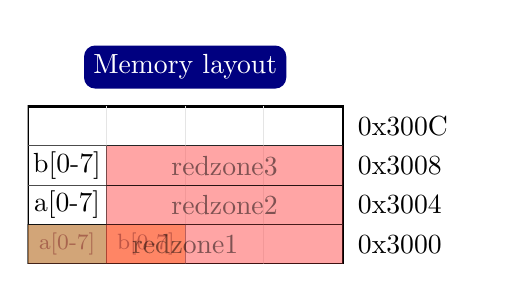
\begin{tikzpicture}
        \clip (0,0) rectangle (6cm, 3cm);
        \memorystack[word size=4,nb blocks=4]
        \onslide<1>{
          \draw[fill=green!70,opacity=0.5] (0.,0.*\stacksizey) rectangle (\stacksizex/4.,1.*\stacksizey) node[midway]{\footnotesize a[0-7]};
          \draw[fill=orange,opacity=0.5] (\stacksizex/4.,0.*\stacksizey) rectangle (\stacksizex/2.,1.*\stacksizey) node[midway]{\footnotesize b[0-7]};
        }
        \memorygoto{2}
        \onslide<2->{
          \draw[fill=red!70,opacity=0.5] (0.,0.*\stacksizey) rectangle (\stacksizex,1.*\stacksizey) node[midway]{redzone1};
          \memorypush{a[0-7]}
          \draw[fill=red!70,opacity=0.5] (0.+\stacksizex/4.,1.*\stacksizey) rectangle (\stacksizex,2.*\stacksizey) node[midway]{redzone2};
          \memorypush{b[0-7]}
          \draw[fill=red!70,opacity=0.5] (0.+\stacksizex/4.,2.*\stacksizey) rectangle (\stacksizex,3.*\stacksizey) node[midway]{redzone3};
        }
      \end{tikzpicture}
    \end{multicols}
    \vspace{1mm}
  \end{exampleblock}
\end{frame}

\begin{frame}[fragile]
  \vspace{-1\baselineskip}
  \begin{columns}
    \column{\textwidth+1cm}
    \scriptsize
    \begin{Verbatim}[commandchars=\\\{\}]
    \ttfamily
\textcolor{teal}{==34015==ERROR: AddressSanitizer: stack-buffer-overflow on address 0x7ffee93ed968 at pc 0x000106812df4 bp 0x7ffee93ed930 sp 0x7ffee93ed928}
\textcolor{blue}{WRITE of size 1 at 0x7ffee93ed968 thread T0}
    #0 0x106812df3 in foo() asan.cpp:4
    #1 0x106812ed8 in main asan.cpp:9
    #2 0x7fff6d3923d4 in start (libdyld.dylib:x86_64+0x163d4)

\textcolor{teal}{Address 0x7ffee93ed968 is located in stack of thread T0 at offset 40 in frame}
    #0 0x106812cdf in foo() asan.cpp:1

  This frame has 2 object(s):
    [32, 40) 'a' (line 2) \textcolor{teal}{<== Memory access at offset 40 overflows this variable}
    [64, 72) 'b' (line 3)
Shadow bytes around the buggy address:
=>0x1fffdd27db20: 00 00 00 00 00 00 00 00 \textcolor{red}{f1 f1 f1 f1} 00[\textcolor{red}{f2}]\textcolor{red}{f2 f2}
  0x1fffdd27db30: 00 \textcolor{red}{f3 f3 f3} 00 00 00 00 00 00 00 00 00 00 00 00
  0x1fffdd27db40: 00 00 00 00 00 00 00 00 00 00 00 00 00 00 00 00
  0x1fffdd27db50: 00 00 00 00 00 00 00 00 00 00 00 00 00 00 00 00
Shadow byte legend (one shadow byte represents 8 application bytes):
  Addressable:           00
  Partially addressable: 01 02 03 04 05 06 07
  Heap left redzone:       \textcolor{red}{fa}
  Freed heap region:       \textcolor{pink}{fd}
  Stack left redzone:      \textcolor{red}{f1}
  Stack mid redzone:       \textcolor{red}{f2}
  Stack right redzone:     \textcolor{red}{f3}
  Stack after return:      \textcolor{pink}{f5}
    \end{Verbatim}
  \end{columns}
\end{frame}

\begin{frame}[fragile]
  \begin{columns}
    \column{\textwidth+1cm}
    \begin{block}{Finding memory leaks with ASan}
      \begin{itemize}
        \item On linux, ASan can display memory leaks
        \item Start executable with \mintinline{bash}{ASAN_OPTIONS=detect_leaks=1 ./myProgram}
      \end{itemize}
    \end{block}
    \scriptsize
    \begin{Verbatim}[commandchars=\\\{\}]
    \ttfamily
\textcolor{red}{==113262==ERROR: LeakSanitizer: detected memory leaks}

\textcolor{blue}{Direct leak of 32 byte(s) in 1 object(s) allocated from:}
  #0 0x7f2671201647 in operator new(unsigned long) /build/dkonst/WORK/build/contrib/gcc-10.1.0/src/gcc/10.1.0/libsanitizer/asan/asan_new_delete.cpp:99
  #1 0x4033c7 in memoryLeak[abi:cxx11]() /afs/cern.ch/user/s/shageboe/asan.cpp:33
  #2 0x403633 in main /afs/cern.ch/user/s/shageboe/asan.cpp:40
  #3 0x7f2670a15492 in __libc_start_main (/lib64/libc.so.6+0x23492)

\textcolor{blue}{Indirect leak of 22 byte(s) in 1 object(s) allocated from:}
  #0 0x7f2671201647 in operator new(unsigned long) /build/dkonst/WORK/build/contrib/gcc-10.1.0/src/gcc/10.1.0/libsanitizer/asan/asan_new_delete.cpp:99
  #1 0x403846 in void std::__cxx11::basic_string<char, std::char_traits<char>, std::allocator<char> >::_M_construct<char const*>(char const*, char const*, std::forward_iterator_tag) /cvmfs/sft.cern.ch/lcg/releases/gcc/10.1.0.c82-6f386/x86_64-centos8/include/c++/10.1.0/bits/basic_string.tcc:219
  #2 0x4033f4 in std::__cxx11::basic_string<char, std::char_traits<char>, std::allocator<char> >::basic_string<std::allocator<char> >(char const*, std::allocator<char> const&) /cvmfs/sft.cern.ch/lcg/releases/gcc/10.1.0.c82-6f386/x86_64-centos8/include/c++/10.1.0/bits/basic_string.h:247
  #3 0x4033f4 in memoryLeak[abi:cxx11]() /afs/cern.ch/user/s/shageboe/asan.cpp:33
  #4 0x403633 in main /afs/cern.ch/user/s/shageboe/asan.cpp:40
  #5 0x7f2670a15492 in __libc_start_main (/lib64/libc.so.6+0x23492)

SUMMARY: AddressSanitizer: 54 byte(s) leaked in 2 allocation(s).
    \end{Verbatim}
  \end{columns}
\end{frame}

\begin{frame}[fragile]
  \frametitle{Address sanitizer (ASan)}
  \begin{block}{Wrap up}
    \begin{itemize}
      \item If a program crashes, run it with asan
      \item Should be part of every \cpp{} continuous integration system
      \item It will also find bugs that by luck didn't crash the program
      \item It doesn't generate false positives
    \end{itemize}
  \end{block}

  \begin{exampleblock}{More info}
    \begin{itemize}
      \item \url{https://github.com/google/sanitizers/wiki/AddressSanitizer}
      \item Compile with asan, and start executable using \mintinline{bash}{ASAN_OPTIONS=help=1 <executable>}
    \end{itemize}
  \end{exampleblock}
\end{frame}

\begin{frame}[fragile]
  \frametitle{Address sanitizer (ASan)}
  \begin{exercise}{address sanitizer}
    \begin{itemize}
      \item Go to \texttt{code/asan}
      \item Compile and run the program \texttt{./asan}
      \item There are two bugs and one memory leak. Use asan to trace them down.
    \end{itemize}
  \end{exercise}

\end{frame}

\begin{frame}[fragile]
  \frametitle{Thread sanitizer (TSan)}
  \begin{block}{TSan}
    \begin{itemize}
      \item Thread sanitizer detects many data races in MT programs
      \item Recompile your program with e.g.\ \mintinline{shell}{clang++ -fsanitize=thread -g -O1 datarace.cpp}
    \end{itemize}
  \end{block}

  \footnotesize
  \begin{verbatim}
% ./a.out
WARNING: ThreadSanitizer: data race (pid=19219)
Write of size 4 at 0x7fcf47b21bc0 by thread T1:
  #0 Thread1 datarace.c:4 (exe+0x00000000a360)

Previous write of size 4 at 0x7fcf47b21bc0 by main thread:
  #0 main datarace.c:10 (exe+0x00000000a3b4)

Thread T1 (running) created at:
  #0 pthread_create tsan_interceptors.cc:705 (exe+0x00000000c790)
  #1 main datarace.c:9 (exe+0x00000000a3a4)
  \end{verbatim}

  \begin{block}{}
    \scriptsize
    \url{https://github.com/google/sanitizers/wiki/ThreadSanitizerCppManual}
  \end{block}
\end{frame}

\begin{frame}[fragile]
  \frametitle{Undefined Behaviour Sanitizer (UBSan)}
  \begin{block}{UBSan}
    \begin{itemize}
      \item Tracks uninitialised memory, broken arithmetic, wrong array indexing and other undefined behaviour
      \item Recompile your program with e.g.\ \mintinline{bash}{clang++ -fsanitize=undefined -g -O1 ub.cpp}
    \end{itemize}
  \end{block}
  \small
  \begin{verbatim}
% ./a.out
up.cpp:3:5: runtime error: signed integer overflow:
            2147483647 + 1 cannot be represented in type 'int'
  \end{verbatim}
  \begin{block}{}
    \footnotesize
    \url{https://clang.llvm.org/docs/UndefinedBehaviorSanitizer.html}
  \end{block}
\end{frame}

  \subsection[valgrind]{The Valgrind family}

\begin{frame}[fragile]
  \frametitle{The valgrind family}
  \begin{block}{Valgrind fundamentals}
    \begin{itemize}
    \item valgrind is a framework for different tools
    \item a processor simulator allowing checks in between instructions
    \item slow (10-50 times slower than normal execution)
    \item easy to use : ``valgrind \textless{}your executable\textgreater''
      \begin{itemize}
      \item no recompilation
      \item better with -g -O0, but not strictly needed
      \end{itemize}
    \item it is free and open source
    \end{itemize}
  \end{block}
  \pause
  \begin{block}{Main tools}
    \begin{description}
      \item[memcheck] a memory checker (default tool) and leak detector
      \item[callgrind] a call graph builder
      \item[helgrind] a race condition detector
    \end{description}
  \end{block}
\end{frame}

\begin{frame}[fragile]
  \frametitle{memcheck}
  \begin{block}{}
    \begin{itemize}
      \item keeps track of all memory allocations and deallocations
      \item is able to detect accesses to unallocated memory
      \item and even tell you when it was deallocated if it was
      \item or what is the closest array in case of overflow
      \item is able to list still allocated memory when program exits\\
        (memory leaks detection)
    \end{itemize}
  \end{block}
\end{frame}

\begin{frame}[fragile]
  \frametitle{valgrind}
  \begin{exercise}{valgrind}
    \begin{itemize}
    \item go to code/valgrind
    \item compile, run, it should work
    \item run with valgrind, see the problem
    \item fix the problem
      \vspace{.3cm}
    \item go back to the code/debug exercise
    \item check it with valgrind
    \item analyze the issue, see that the variance was biaised
    \item fix the issue
    \end{itemize}
  \end{exercise}
\end{frame}

\begin{frame}[fragile]
  \frametitle{memcheck}
  \begin{exercise}{memcheck}
    \begin{itemize}
    \item go to code/memcheck
    \item compile, run, it should work
    \item run with valgrind, see LEAK summary
    \item run with -{}-leak-check=full to get details
    \item analyze and correct it
    \end{itemize}
  \end{exercise}
\end{frame}

\begin{frame}[fragile]
  \frametitle{callgrind and kcachegrind}
  \begin{block}{callgrind}
    \begin{itemize}
      \item keeps track of all function calls
      \item and time spent in each function
      \item build statistics on calls, CPU usages and more
      \item outputs flat statistics file, quite unreadable
    \end{itemize}
  \end{block}
  \begin{block}{kcachegrind}
    \begin{itemize}
      \item a gui exploiting statistics built by callgrind
      \item able to browse graphically the program calls
      \item able to ``graph'' CPU usage on the program structure
    \end{itemize}
  \end{block}
\end{frame}

\begin{frame}[fragile]
  \frametitle{callgrind}
  \begin{exercise}{callgrind}
    \begin{itemize}
    \item go to code/callgrind
    \item compile, run, it will be slow
    \item change nb iterations to 20
    \item run with valgrind -{}-tool=callgrind
    \item look at output with kcachegrind
    \item change fibo call to fibo2
    \item observe the change in kcachegrind
    \end{itemize}
  \end{exercise}
\end{frame}

\begin{frame}[fragile]
  \frametitle{helgrind}
  \begin{block}{}
    \begin{itemize}
      \item keeps track of all pthreads activity
      \item in particular keeps track of all mutexes
      \item builds a graph of dependencies of the different actions
      \item works on the resulting graph to detect:
        \begin{itemize}
        \item possible dead locks
        \item possible data races
        \end{itemize}
    \end{itemize}
  \end{block}
  \pause
  \begin{alertblock}{}
    Note the ``possible''. It finds future problems !
  \end{alertblock}
\end{frame}

\begin{frame}[fragile]
  \frametitle{helgrind}
  \begin{exercise}{helgrind}
    \begin{itemize}
    \item go to code/helgrind
    \item compile, run
    \item check it with valgrind. You may see strange behavior \\
      or it will be perfectly fine
    \item check it with valgrind -{}-tool=helgrind
    \item understand issue and fix
    \end{itemize}
  \end{exercise}
\end{frame}

  \subsection[static]{Static code analysis}

\begin{frame}[fragile]
  \frametitle{Static analysis}
  \begin{alertblock}{The problem}
    \begin{itemize}
    \item all the tools discussed so far work on binaries
    \item they analyze the code being run
    \item so there is a coverage problem (e.g. for error cases)
    \end{itemize}
  \end{alertblock}
  \pause
  \begin{block}{A (partial) solution : analyzing the source code}
    \begin{itemize}
    \item build a graph of dependencies of the calls
    \item use graph tools to detect potential memory corruptions,
      memory leaks or missing initializations
    \end{itemize}
  \end{block}
  \pause
  \begin{block}{Existing tools}
    \begin{description}
    \item[\href{http://www.coverity.com/}{\beamergotobutton{Coverity}}]
      proprietary tool, the most complete
    \item[\href{http://cppcheck.sourceforge.net/}{\beamergotobutton{cppcheck}}]
      free and opensource, but less complete
    \item[\href{https://clang.llvm.org/extra/clang-tidy/}{\beamergotobutton{clang-tidy}}]
      clang-based ``linter'', includes clang static analyzer
    \end{description}
  \end{block}
\end{frame}

\begin{frame}[fragile]
  \frametitle{cppcheck}
  \begin{exercise}{cppcheck}
    \begin{itemize}
    \item go to code/cppcheck
    \item compile, run, see that it works
    \item use valgrind: no issue
    \item use cppcheck, see the problem
    \item analyze the issue, and fix it
    \item bonus: understand why valgrind did not complain \\
      and how the standard deviation could be biased \\
      hint : use gdb and check addresses of v and diffs
    \end{itemize}
  \end{exercise}
\end{frame}

\begin{frame}[fragile]
  \frametitle{clang-tidy}
  \begin{block}{Documentation and supported checks}
    \begin{itemize}
      \item \url{https://clang.llvm.org/extra/clang-tidy/}
    \end{itemize}
  \end{block}
  \begin{block}{Run clang-tidy}
    \begin{itemize}
      \item \mintinline{bash}{clang-tidy <file.cpp> -checks=...}
      \item \mintinline{bash}{clang-tidy <file.cpp>} (checks from .clang-tidy file)
      \item \mintinline{bash}{clang-tidy <file.cpp> --fix} (applies fixes)

    \end{itemize}
  \end{block}
  \begin{block}{Compilation flags}
    \begin{itemize}
      \item clang-tidy needs to know exactly how your program is built
      \item \mintinline{bash}{clang-tidy ... -- <all compiler flags>}
    \end{itemize}
  \end{block}
  \begin{block}{.clang-tidy file}
    \begin{itemize}
      \item describes which checks to run
      \item usually checked in at repository root
    \end{itemize}
  \end{block}
\end{frame}

\begin{frame}[fragile]
  \begin{block}{Automatically collecting compilation flags}
    \begin{itemize}
      \item clang-tidy looks for a file called compile\_commands.json
      \item contains the exact build flags for each .cpp file
      \item generate with CMake: \\
        \mintinline{bash}{cmake -DCMAKE_EXPORT_COMPILE_COMMANDS=ON ...}
      \item for Makefiles try \href{https://github.com/rizsotto/Bear}{\beamergotobutton{Bear}}
      \item allows to run clang-tidy in bulk on all files:
      \begin{itemize}
        \item \mintinline{bash}{run-clang-tidy -checks ...}
        \item \mintinline{bash}{run-clang-tidy} (checks from .clang-tidy)
        \item \mintinline{bash}{run-clang-tidy -fix} (applies fixes)
      \end{itemize}
    \end{itemize}
  \end{block}
\end{frame}

\begin{frame}[fragile]
  \frametitle{clang-tidy}
  \begin{exercise}{clang-tidy}
    \begin{itemize}
      \item go to any example which compiles (e.g. code/cppcheck)
      \item \mintinline{bash}{mkdir build && cd build}
      \item \mintinline{bash}{cmake -DCMAKE_EXPORT_COMPILE_COMMANDS=ON ..}
      \item \mintinline{bash}{clang-tidy <../file.cpp> -checks=*}
      \item inspect output
      \item run with \mintinline{bash}{--fix} flag
      \item revert changes using \mintinline{bash}{git checkout <../file.cpp>}
    \end{itemize}
  \end{exercise}
\end{frame}

  \subsection[prof]{Profiling}

\begin{frame}[fragile]
  \frametitle{Profiling}
  \begin{block}{Conceptually}
    \begin{itemize}
      \item take a measurement of a performance aspect of a program
      \begin{itemize}
        \item where in my code is most of the time spent?
        \item is my program compute or memory bound?
        \item does my program make good use of the cache?
        \item is my program using all cores most of the time?
        \item how often are threads blocked and why?
        \item which API calls are made and in which order?
        \item ...
      \end{itemize}
      \item the goal is to find performance bottlenecks
      \item is usually done on a compiled program, not on source code
    \end{itemize}
  \end{block}
\end{frame}

\begin{frame}[fragile]
  \frametitle{perf, VTune and uProf}
  \begin{block}{perf}
    \begin{itemize}
      \item perf is a powerful command line profiling tool for linux
      \item compile with \mintinline{bash}{-g -fno-omit-frame-pointer}
      \item \mintinline{bash}{perf stat -d <prg>} gathers performance statistics while running \mintinline{bash}{<prg>}
      \item \mintinline{bash}{perf record -g <prg>} starts profiling \mintinline{bash}{<prg>}
      \item \mintinline{bash}{perf report} displays a report from the last profile
      \item More information in \href{https://perf.wiki.kernel.org/index.php/Main_Page}{this wiki}, \href{https://www.brendangregg.com/linuxperf.html}{this website} or \href{https://indico.cern.ch/event/980497/contributions/4130271/attachments/2161581/3647235/linux-systems-performance.pdf}{this talk}.
    \end{itemize}
  \end{block}
  \begin{block}{Intel VTune and AMD uProf}
    \begin{itemize}
      \item Graphical profilers from CPU vendors with rich features
      \item Needs vendor's CPU for full experience
      \item More information on \href{https://www.intel.com/content/www/us/en/developer/tools/oneapi/vtune-profiler.html}{Intel's website} and \href{https://developer.amd.com/amd-uprof/}{AMD's website}
    \end{itemize}
  \end{block}
\end{frame}

  \subsection[doxygen]{Doxygen}

\begin{frame}[fragile]
  \frametitle{Doxygen}
  \begin{block}{Doxygen}
    \begin{itemize}
      \item Generates documentation from source code comments
      \item Output formats: HTML, LaTeX, XML, ...
      \begin{itemize}
        \item May be input for further generators, e.g.\ Sphinx
      \end{itemize}
      \item Doxygen uses a config file, usually called Doxyfile
      \item Run \mintinline{bash}{doxygen -g} to generate an initial Doxyfile
      \item Edit Doxyfile (e.g.\ output format, source code location, etc.)
      \item Run \mintinline{bash}{doxygen} to (re-)generate documentation
      \item View e.g.\ HTML documentation using a standard web browser
      \item More on the \href{https://doxygen.nl/manual/starting.html}{doxygen website}
    \end{itemize}
  \end{block}
\end{frame}

\begin{frame}[fragile]
  \frametitle{Doxygen}
  \begin{block}{Comment blocks}
    \begin{columns}
      \begin{column}{.35\textwidth}
        \begin{cppcode*}{}
          /**
           * text/directives ...
           */
          some_cpp_entity

          /*!
           * text/directives ...
           */
          some_cpp_entity
        \end{cppcode*}
      \end{column}
      \begin{column}{.35\textwidth}
        \begin{cppcode*}{firstnumber=10}
          ///
          /// text/directives ...
          ///
          some_cpp_entity

          //!
          //! text/directives ...
          //!
          some_cpp_entity
        \end{cppcode*}
      \end{column}
    \end{columns}
    \begin{itemize}
      \item More details available \href{https://www.doxygen.nl/manual/docblocks.html}{here}
    \end{itemize}
  \end{block}
  \begin{block}{Comment blocks for members}
    \begin{cppcode*}{linenos=false}
      int a_class_member; ///< trailing documentation
    \end{cppcode*}
  \end{block}

\end{frame}

\begin{frame}[fragile]
  \frametitle{Doxygen}
  \begin{block}{Comment directives}
    \begin{cppcode*}{}
      /**
       * Long description here. May include HTML etc.
       *
       * \brief Checks whether i is odd
       * \tparam Integral The integral type of the input
       * \param i Input value
       * \return True if i is odd, otherwise false
       * \throw std::out_of_range if i is larger than 100
       * \see isEven
       */
      template <typename Integral>
      bool isOdd(Integral i);
    \end{cppcode*}
    \begin{itemize}
      \item All directives can also start with @ instead of \textbackslash
      \item A list of all commands can be found \href{https://doxygen.nl/manual/commands.html}{here}
    \end{itemize}
  \end{block}
\end{frame}


  \section[conc]{Concurrency}
  \subsection[thr]{Threads and async}

\begin{frame}[fragile]
  \frametitlecpp[11]{Basic concurrency}
  \begin{block}{Threading}
    \begin{itemize}
    \item \cpp11 added \mintinline{cpp}{std::thread} in \mintinline{cpp}{<thread>} header
    \item takes a function as argument of its constructor
    \item must be detached or joined before the main thread terminates
    \item \cpp20: \mintinline{cpp}{std::jthread} automatically joins at destruction
    \end{itemize}
  \end{block}
  \pause
  \begin{exampleblock}{Example code}
    \begin{cppcode*}{}
      void foo() {...}
      void bar() {...}
      int main() {
        std::thread t1{foo};
        std::thread t2{bar};
        for (auto t: {&t1,&t2}) t->join();
      }
    \end{cppcode*}
  \end{exampleblock}
\end{frame}

\begin{frame}[fragile]
  \frametitlecpp[11]{The thread constructor}
  \begin{exampleblock}{Can take a function and its arguments}
    \begin{cppcode*}{}
      void function(int j, double j) {...};
      std::thread t1{function, 1, 2.0};
    \end{cppcode*}
  \end{exampleblock}
  \pause
  \begin{exampleblock}{Can take any function-like object}
    \begin{cppcode*}{}
      struct AdderFunctor {
        AdderFunctor(int i): m_i(i) {}
        int operator() (int j) const { return m_i+j; }
        int m_i;
      };
      std::thread t2{AdderFunctor{2}, 5};
      int a;
      std::thread t3{[](int i) { return i+2; }, a};
      std::thread t4{[a]       { return a+2; }};
    \end{cppcode*}
  \end{exampleblock}
\end{frame}

\begin{frame}[fragile]
  \frametitlecpp[11]{Basic asynchronicity}
  \begin{block}{Concept}
    \begin{itemize}
    \item separation of the specification of what should be done and the retrieval of the results
    \item ``start working on this, and let me check if it's done''
    \end{itemize}
  \end{block}
  \pause
  \begin{block}{Practically}
    \begin{itemize}
    \item \mintinline{cpp}{std::async} function launches an asynchronous task
    \item \mintinline{cpp}{std::future<T>} allows to retrieve the result
    \end{itemize}
  \end{block}
  \pause
  \begin{exampleblock}{Example code}
    \begin{cppcode*}{}
      int f() {...}
      std::future<int> res = std::async(f);
      std::cout << res.get() << "\n";
    \end{cppcode*}
  \end{exampleblock}
\end{frame}

\begin{frame}[fragile]
  \frametitlecpp[11]{Mixing the two}
  \begin{block}{Is async running concurrently ?}
    \begin{itemize}
    \item it depends!
    \item you can control this with a launch policy argument
      \begin{description}
      \item[std::launch::async] start executing immediately on a separate thread (may be a new thread, a thread pool, ...)
      \item[std::launch::deferred] causes lazy execution in current thread
      \end{description}
      \begin{itemize}
      \item execution starts when \mintinline{cpp}{get()} is called on the returned future
      \end{itemize}
    \item default is not specified, but tries to use existing concurrency!
    \end{itemize}
  \end{block}
  \pause
  \begin{exampleblock}{Usage}
    \begin{cppcode*}{}
      int f() {...}
      auto res1 = std::async(std::launch::async, f);
      auto res2 = std::async(std::launch::deferred, f);
    \end{cppcode*}
  \end{exampleblock}
\end{frame}

\begin{frame}[fragile]
  \frametitlecpp[11]{Fine-grained control on asynchronous execution}
  \begin{block}{\texttt{std::packaged\_task} template}
    \begin{itemize}
    \item creates an asynchronous version of any function-like object
      \begin{itemize}
      \item identical arguments
      \item returns a \mintinline{cpp}{std::future}
      \end{itemize}
    \item provides access to the returned future
    \item associated with threads, gives full control on execution
    \end{itemize}
  \end{block}
  \pause
  \begin{exampleblock}{Usage}
    \begin{cppcode*}{}
      int f() { return 42; }
      std::packaged_task<int()> task{f};
      auto future = task.get_future();
      task();
      std::cout << future.get() << std::endl;
    \end{cppcode*}
  \end{exampleblock}
\end{frame}

  \subsection[mutex]{Mutexes}

\begin{frame}[fragile]
  \frametitlecpp[11]{Races}
  \begin{exampleblock}{Example code}
    \begin{cppcode*}{}
      int a = 0;
      void inc() { a++; };
      void inc100() {
        for (int i=0; i < 100; i++) inc();
      };
      int main() {
        std::thread t1(inc100);
        std::thread t2(inc100);
        for (auto t: {&t1,&t2}) t->join();
        std::cout << a << std::endl;
      }
    \end{cppcode*}
  \end{exampleblock}
  \pause
  \begin{block}{What do you expect ? Try it in code/race}
    \pause
    Anything between 100 and 200 !!!
  \end{block}
\end{frame}

\begin{frame}[fragile]
  \frametitlecpp[11]{Atomicity}
  \begin{exampleblock}{Definition (wikipedia)}
    \begin{itemize}
    \item an operation (or set of operations) is atomic if it appears to the rest of the system to occur instantaneously
    \end{itemize}
  \end{exampleblock}
  \begin{block}{Practically}
    \begin{itemize}
    \item an operation that won't run concurrently to another one
    \item an operation that will have a stable environment during execution
    \end{itemize}
  \end{block}
  \pause
  \begin{alertblock}{Is \texttt{++} operator atomic ?}
    \pause
    Usually not. It behaves like :
    \begin{cppcode*}{}
      eax = a       // memory to register copy
      increase eax  // increase (atomic CPU instruction)
      a = eax       // copy back to memory
    \end{cppcode*}
  \end{alertblock}
\end{frame}

\begin{frame}[fragile]
  \frametitlecpp[11]{Timing}
  \begin{exampleblock}{Code}
    \begin{cppcode*}{}
      eax = a       // memory to register copy
      increase eax  // increase (atomic CPU instruction)
      a = eax       // copy back to memory
    \end{cppcode*}
  \end{exampleblock}
  \begin{block}{For 2 threads}
    \begin{tikzpicture}
      \begin{umlseqdiag}
        \umlobject[x=0, class=eax]{Thread 1}
        \umlobject[x=3, class=a, fill=blue!20]{Memory}
        \umlobject[x=6, class=eax]{Thread 2}
        \begin{umlcall}[op=read, type=synchron, return=0]{Thread 1}{Memory}
        \end{umlcall}
        \begin{umlcall}[padding=3, op=read, type=synchron, return=0]{Thread 2}{Memory}
        \end{umlcall}
        \begin{umlcallself}[op=incr, type=synchron]{Thread 1}
        \end{umlcallself}
        \begin{umlcallself}[op=incr, type=synchron]{Thread 2}
        \end{umlcallself}
        \begin{umlcall}[op=write 1]{Thread 2}{Memory}
        \end{umlcall}
        \begin{umlcall}[padding=3, op=write 1]{Thread 1}{Memory}
        \end{umlcall}
      \end{umlseqdiag}
      \draw[-triangle 60](8.5,0) -- (8.5,-4) node[right, pos=0.5]{time};
    \end{tikzpicture}
  \end{block}
\end{frame}

\begin{frame}[fragile]
  \frametitlecpp[17]{Mutexes and Locks}
  \begin{block}{Concept}
    \begin{itemize}
    \item Use locks to serialize access to a non-atomic piece of code
    \end{itemize}
  \end{block}
  \pause
  \begin{block}{The objects}
    \begin{description}[labelwidth=1.8cm]
    \item[std::mutex] in the \mintinline{cpp}{mutex} header. \textbf{Mut}ual \textbf{ex}clusion
    \item[std::scoped\_lock] RAII to lock and unlock automatically
    \item[std::unique\_lock] same, but can be released/relocked explicitly
    \end{description}
  \end{block}
  \pause
  \begin{exampleblock}{Practically}
    \begin{cppcode*}{}
      int a = 0;
      std::mutex m;
      void inc() {
        std::scoped_lock lock{m};
        a++;
      }
    \end{cppcode*}
  \end{exampleblock}
\end{frame}

\begin{frame}[fragile]
  \frametitlecpp[17]{Mutexes and Locks}
  \begin{goodpractice}{Locking}
    \begin{itemize}
      \item Generally, use \mintinline{cpp}{std::scoped_lock}. Before \cpp17 use \mintinline{cpp}{std::lock_guard}.
      \item Hold as short as possible, consider wrapping critical section in block statement \mintinline{cpp}|{ }|
      \item Only if manual control needed, use \mintinline{cpp}{std::unique_lock}
    \end{itemize}
  \end{goodpractice}
  \begin{exampleblock}{}
    \begin{cppcode*}{gobble=2}
      void function(...) {
        // ...
        {
          std::scoped_lock myLocks{mutex1, mutex2, ...};
          // critical section
        }
      }
    \end{cppcode*}
  \end{exampleblock}
\end{frame}

\begin{frame}[fragile]
  \frametitle{Mutexes and Locks}
  \begin{alertblock}{Exercise Time}
    \begin{itemize}
    \item Go to code/race
    \item Look at the code and try it\\
      See that it has a race condition
    \item Use a mutex to fix the issue
    \item See the difference in execution time
    \end{itemize}
  \end{alertblock}
\end{frame}

\begin{frame}[fragile]
  \frametitlecpp[11]{Dead lock}
  \begin{exampleblock}{Scenario}
    \begin{itemize}
    \item 2 mutexes, 2 threads
    \item locking order different in the 2 threads
    \end{itemize}
  \end{exampleblock}
  \pause
  \begin{block}{Sequence diagram}
    \begin{tikzpicture}
      \begin{umlseqdiag}
        \umlobject[x=0]{Thread 1}
        \umlobject[x=2.5, fill=blue!20]{Mutex A}
        \umlobject[x=5, fill=blue!20]{Mutex B}
        \umlobject[x=7.5]{Thread 2}
        \begin{umlcall}[op=lock]{Thread 1}{Mutex A}
        \end{umlcall}
        \begin{umlcall}[op=lock, dt=6]{Thread 2}{Mutex B}
        \end{umlcall}
        \begin{umlcall}[op=lock (block), dt=6]{Thread 1}{Mutex B}
        \end{umlcall}
        \begin{umlcall}[op=lock (block), dt=12]{Thread 2}{Mutex A}
        \end{umlcall}
      \end{umlseqdiag}
      \draw[-triangle 60](9,0) -- (9,-4) node[right, pos=0.5]{time};
    \end{tikzpicture}
  \end{block}
\end{frame}

\begin{frame}[fragile]
  \frametitlecpp[11]{How to avoid dead locks}
  \begin{block}{Possible solutions}
    \begin{itemize}
    \item \cpp17: \mintinline{cpp}{std::scoped_lock lock{m1, m2};} comes with deadlock-avoidance algorithm
    \item Never take several locks
      \begin{itemize}
      \item Or add master lock protecting the locking phase
      \end{itemize}
    \item Respect a strict order in the locking across all threads
    \item Do not use locks
      \begin{itemize}
      \item Use other techniques, e.g. lock-free queues
      \end{itemize}
    \end{itemize}
  \end{block}
\end{frame}

\begin{frame}[fragile]
  \frametitlecpp[17]{Shared mutex / locks}
  \begin{block}{Sharing a mutex}
    \begin{itemize}
      \item Normal \mintinline{cpp}{std::mutex} objects cannot be shared
      \item \mintinline{cpp}{std::shared_mutex} to the rescue, but can be slower
      \item \emph{Either} exclusive \emph{or} shared locking; never both
    \end{itemize}
  \end{block}
  \begin{exampleblock}{}
    \begin{cppcode*}{gobble=2}
      Data data; std::shared_mutex mutex;
      auto reader = [&](){
        std::shared_lock lock{mutex};
        read(data); // Many can read
      };
      std::thread r1{reader}, r2{reader}, ...;

      std::thread writer([&](){
        std::scoped_lock lock{mutex}; // exclusive
        modify(data); // Only one can write
      });
    \end{cppcode*}
  \end{exampleblock}
\end{frame}

  \subsection[atomic]{Atomic types}

\begin{frame}[fragile]
  \frametitlecpp[11]{Atomic types in \cpp}
  \begin{block}{\texttt{std::atomic} template}
    \begin{itemize}
      \item Any trivially copyable type can be made atomic in C++
      \item Most useful for integral types
      \item May internally use locks for custom types
    \end{itemize}
  \end{block}
  \begin{exampleblock}{}
    \begin{cppcode*}{}
      std::atomic<int> a{0};
      std::thread t1([&](){ a++; });
      std::thread t2([&](){ a++; });
      a += 2;
      t1.join(); t2.join();
      assert( a == 4 ); // Guaranteed to succeed
    \end{cppcode*}
  \end{exampleblock}
\end{frame}

\begin{frame}[fragile]
  \begin{alertblock}{Expressions using an atomic type are \textit{not} atomic!}
    \begin{itemize}
      \item Atomic load; value+2; atomic store
    \end{itemize}
    \begin{cppcode*}{}
      std::atomic<int> a{0};
      std::thread t1([&]{ a = a + 2; });
      std::thread t2([&]{ a = a + 2; });
    \end{cppcode*}
  \end{alertblock}
  \begin{block}{Sequence diagram}
    \begin{tikzpicture}
      \begin{umlseqdiag}
        \umlobject[x=0]{Thread 1}
        \umlobject[x=3, fill=blue!20]{atomic}
        \umlobject[x=6]{Thread 2}
        \begin{umlcall}[op=load]{Thread 1}{atomic}
        \end{umlcall}
        \begin{umlcall}[op=+2]{Thread 1}{Thread 1}
        \end{umlcall}
        \begin{umlcall}[op=load]{Thread 2}{atomic}
        \end{umlcall}
        \begin{umlcall}[op=+2]{Thread 2}{Thread 2}
        \end{umlcall}
        \begin{umlcall}[op=store 2]{Thread 1}{atomic}
        \end{umlcall}
        \begin{umlcall}[op=store 2]{Thread 2}{atomic}
        \end{umlcall}
      \end{umlseqdiag}
      \draw[-triangle 60](9,0) -- (9,-4) node[right, pos=0.5]{time};
    \end{tikzpicture}
  \end{block}
\end{frame}

\begin{frame}[fragile]
  \begin{block}{Use atomic member functions}
    \begin{itemize}
      \item The member functions of \mintinline{cpp}{std::atomic} are thread safe
      \item \mintinline{cpp}{fetch_add} and \mintinline{cpp}{operator+=}: atomic \{ load; add; store \}
      \item But don't confuse ``\mintinline{cpp}{a += 2}'' and ``\mintinline{cpp}{a = a + 2}''
    \end{itemize}
  \end{block}
  \begin{exampleblock}{}
    \begin{cppcode*}{}
      std::atomic<int> a{0};
      std::thread t1([&]{ a.fetch_add(2); });
      std::thread t2([&]{ a += 2; });
    \end{cppcode*}
  \end{exampleblock}
  \begin{block}{Sequence diagram}
    \begin{tikzpicture}
      \begin{umlseqdiag}
        \umlobject[x=0]{Thread 1}
        \umlobject[x=3, fill=blue!20]{atomic}
        \umlobject[x=6]{Thread 2}
        \begin{umlcall}[op=fetch\_add]{Thread 1}{atomic}
        \end{umlcall}
        \begin{umlcall}[op=\texttt{+=}, dt=9]{Thread 2}{atomic}
        \end{umlcall}
      \end{umlseqdiag}
      \draw[-triangle 60](9,0) -- (9,-2) node[right, pos=0.5]{time};
    \end{tikzpicture}
  \end{block}
\end{frame}

\begin{frame}[fragile]
  \frametitlecpp[20]{Atomic references}
  \begin{block}{\texttt{std::atomic\_ref} template}
    \begin{itemize}
      \item Wraps a \mintinline{cpp}{T&} and makes access to it atomic
      \item Like \mintinline{cpp}{std::atomic<T>}, but does not contain the \mintinline{cpp}{T}
    \end{itemize}
  \end{block}
  \begin{exampleblock}{}
    \begin{cppcode*}{gobble=2}
      int a{0};
      std::thread t1([&]{ std::atomic_ref<int> r{a}; r++;});
      std::thread t2([&]{ std::atomic_ref{a}++; });
      t1.join(); t2.join();
      a += 2; // non-atomic (fine, threads joined before)
      assert( a == 4 ); // Guaranteed to succeed
    \end{cppcode*}
  \end{exampleblock}
  \begin{alertblock}{Don't mix concurrent atomic and non-atomic access}
    \begin{cppcode*}{gobble=2}
      std::thread t3([&]{ std::atomic_ref{a}++; });
      a += 2; // data race
      t3.join();
    \end{cppcode*}
  \end{alertblock}
\end{frame}

\begin{frame}[fragile]
  \frametitle{Atomic types in \cpp}
  \begin{exercise}{Atomics}
    \begin{itemize}
      \item Go to \texttt{code/atomic}
      \item You'll find a program with the same race condition as in \texttt{race}
      \item Fix it using \mintinline{cpp}{std::atomic}
    \end{itemize}
  \end{exercise}
\end{frame}

  \subsection[TLS]{Thread-local storage}

\begin{frame}[fragile]
  \frametitlecpp[20]{Thread-local storage}
  \begin{block}{\mintinline{cpp}{thread_local} keyword}
    \begin{itemize}
      \item A variable can be declared \mintinline{cpp}{thread-local}
      \item Then every thread will have its own copy
      \item Most useful for ``working memory'' in each thread
      \item Note: Can also be declared directly on the stack of a thread
      \begin{itemize}
        \item and will be faster, thus should be preferred when possible
      \end{itemize}
    \end{itemize}
  \end{block}
  \begin{exampleblock}{}
    \begin{cppcode*}{}
      thread_local int a{0};
      std::jthread t1([&] { a++; });
      std::jthread t2([&] { a++; });
      a += 2;
      t1.join(); t2.join();
      assert( a == 2 ); // Guaranteed to succeed
    \end{cppcode*}
  \end{exampleblock}
\end{frame}

  \subsection[condition]{Condition Variables}

\begin{frame}[fragile]
  \frametitlecpp[11]{Condition variables}
  \begin{block}{Communicating between threads}
    \begin{itemize}
      \item Take the case where threads are waiting for other thread(s)
      \item \cppinline{std::condition_variable}
      \begin{itemize}
        \item from \cppinline{<condition_variable>} header
      \end{itemize}
      \item Allows for a thread to sleep (= conserve CPU time) until a given condition is satisfied
    \end{itemize}
  \end{block}
  \pause
  \begin{block}{Usage}
    \begin{itemize}
    \item Use RAII-style locks to protect shared data
    \item \cppinline{wait()} will block until the condition is met
      \begin{itemize}
      \item you can have several waiters sharing the same mutex
      \end{itemize}
    \item \cppinline{notify_one()} will wake up one waiter
    \item \cppinline{notify_all()} will wake up all waiters
    \end{itemize}
  \end{block}
\end{frame}

\begin{frame}[fragile]
  \frametitlecpp[17]{Using condition variables: notify}
  \begin{block}{Producer side: providing data to waiting threads}
    \begin{itemize}
      \item Protect data with a mutex, and use condition variable to notify consumers
      \item Optimal use: don't hold lock while notifying
      \begin{itemize}
        \item waiting threads would be blocked
      \end{itemize}
    \end{itemize}
  \end{block}
  \begin{exampleblock}{}
    \begin{cppcode*}{}
      std::mutex mutex;
      std::condition_variable cond;
      Data data;
      std::thread producer([&](){
        {
          std::scoped_lock lock{mutex};
          data = produceData(); // may take long ...
        }
        cond.notify_all();
      });
    \end{cppcode*}
  \end{exampleblock}
\end{frame}

\begin{frame}[fragile]
  \frametitlecpp[11]{Using condition variables: wait}
  \vspace{-1.2\baselineskip}
  \begin{overprint}
  \onslide<1>
  \begin{block}{Mechanics of wait}
    \begin{itemize}
      \item Many threads are waiting for shared data
      \item Pass a \cppinline{unique_lock} and a predicate for wakeup to \cppinline{wait()}
      \item \cppinline{wait()} sends threads to sleep while predicate is \cppinline{false}
      \item \cppinline{wait()} will only lock when necessary; unlocked while sleeping
      \item Threads might wake up spuriously, but \cppinline{wait()} returns only when lock available \emph{and} predicate \cppinline{true}
    \end{itemize}
  \end{block}
  \onslide<2->
  \begin{block}{Waiting / waking up}
    \begin{itemize}
      \item \cppinline{notify_all()} is called, threads wake up
      \item Threads try to lock mutex, and evaluate predicate
      \item One thread succeeds to acquire mutex, starts data processing
      \item {\color{red} Problem}: Thread holds mutex now, other threads are blocked!
    \end{itemize}
  \end{block}
  \end{overprint}

  \begin{alertblock}{Na\"ive waiting}
    \begin{cppcode*}{gobble=2,highlightlines=3}
      auto processData = [&](){
        std::unique_lock<std::mutex> lock{mutex};
        cond.wait(lock, [&](){ return data.isReady(); });
        process(data);
      };
    \end{cppcode*}
  \end{alertblock}
\end{frame}

\begin{frame}[fragile]
  \frametitlecpp[11]{Using condition variables: correct wait}
  \begin{block}{Waiting / waking up}
    \begin{itemize}
      \item {\color{green!50!black} Solution:} Put locking and waiting in a scope
      \item Threads will one-by-one wake up, acquire lock, evaluate predicate, release lock
    \end{itemize}
  \end{block}

  \begin{exampleblock}{Correct waiting}
    \begin{cppcode*}{gobble=2}
      auto processData = [&](){
        {
          std::unique_lock<std::mutex> lock{mutex};
          cond.wait(lock, [&](){ return data.isReady(); });
        }
        process(data);
      };
      std::thread t1{processData}, t2{processData}, ...;
      for (auto t : {&producer, &t1, &t2, ...}) t->join();
    \end{cppcode*}
  \end{exampleblock}
\end{frame}

\begin{frame}[fragile]
  \frametitle{Condition variables}
  \begin{exerciseWithShortcut}{Condition variables}{Condition vars}
    \begin{itemize}
    \item Go to \texttt{exercises/condition\_variable}
    \item Look at the code and run it\\
      See that it has a race condition
    \item Fix the race condition in the usage of the condition variable
    \item Try to make threads process data in parallel
    \end{itemize}
  \end{exerciseWithShortcut}
\end{frame}


  \section[py]{\cpp and python}
  \subsection[module]{Writing a module}

\begin{frame}[fragile]
  \frametitle{How to build a python 3 module around \cpp code}
  \begin{block}{\cpp code : mandel.hpp}
    \begin{cppcode*}{}
      int mandel(Complex const & a);
    \end{cppcode*}
  \end{block}
\end{frame}

\begin{frame}[fragile]
  \frametitle{Basic Module(1): wrap your method}
  \begin{block}{mandelModule.cpp - see exercises/python exercise}
    \begin{cppcode*}{}
      #include <Python.h>
      #include "mandel.hpp"
      PyObject * mandel_wrapper(PyObject * self,
                                PyObject * args) {
        // Parse Input
        float r, i;
        if (!PyArg_ParseTuple(args, "ff", &r, &i))
          return nullptr;
        // Call C++ function
        int result = mandel(Complex(r, i));
        // Build returned objects
        return PyLong_FromLong(result);
      }
    \end{cppcode*}
  \end{block}
\end{frame}

\begin{frame}[fragile]
  \frametitle{Basic Module(2): create the python module}
  \begin{block}{mandelModule.cpp - see exercises/python exercise}
    \begin{cppcode*}{}
      // declare the modules' methods
      PyMethodDef mandelMethods[] = {
          {"mandel", mandel_wrapper, METH_VARARGS,
          "computes nb of iterations for mandelbrot set"},
          {nullptr, nullptr, 0, nullptr}
      };
      // declare the module
      struct PyModuleDef mandelModule = {
        PyModuleDef_HEAD_INIT,
        "mandel", nullptr, -1, mandelMethods
      };
      PyMODINIT_FUNC PyInit_mandel() {
        return PyModule_Create(&mandelModule);
      }
    \end{cppcode*}
  \end{block}
\end{frame}

\begin{frame}[fragile]
  \frametitle{Basic Module(3): use it}
  \begin{block}{First compile the module}
    \begin{itemize}
    \item as a regular shared library
    \item with '\mintinline{bash}{-I \$(PYTHON\_INCLUDE)}'
    \end{itemize}
  \end{block}
  \begin{block}{mandel.py - see exercises/python exercise}
    \begin{minted}[gobble=4]{python}
      from mandel import mandel
      v = mandel(0.7, 1.2)
    \end{minted}
  \end{block}
\end{frame}

  \subsection[C]{Marrying \cpp and C}

\begin{frame}[fragile]
  \frametitle{A question of mangling}
  \begin{block}{Mangling}
    the act of converting the name of variable or function to a symbol name in the binary code
  \end{block}
  \begin{block}{C versus \cpp symbol names}
    \begin{itemize}
    \item C uses bare function name
    \item \cpp allows overloading of functions by taking the signature into account
    \item so \cpp mangling has to contain signature
    \end{itemize}
  \end{block}
\end{frame}

\begin{frame}[fragile]
  \frametitle{C mangling}
  \begin{exampleblock}{Source : file.c}
    \begin{cppcode*}{}
      float sum(float a, float b);
      int square(int a);
      // won't compile : conflicting types for ‘square’
      // float square(float a);
    \end{cppcode*}
  \end{exampleblock}
  \begin{block}{Binary symbols : file.o}
    \begin{minted}{shell}
      # nm file.o
      000000000000001a T square
      0000000000000000 T sum
    \end{minted}
  \end{block}
\end{frame}

\begin{frame}[fragile]
  \frametitle{\cpp mangling}
  \begin{exampleblock}{Source : file.cpp}
    \begin{cppcode*}{}
      float sum(float a, float b);
      int square(int a);
      // ok, signature is different
      float square(float a);
    \end{cppcode*}
  \end{exampleblock}
  \begin{block}{Binary symbols : file.o}
    \begin{minted}{shell}
      # nm file.o
      0000000000000000 T _Z3sumff
      000000000000002a T _Z6squaref
      000000000000001a T _Z6squarei
    \end{minted}
  \end{block}
\end{frame}

\begin{frame}[fragile]
  \frametitle{Forcing C mangling in \cpp}
  \begin{block}{extern ``C''}
    These functions will use C mangling :
    \begin{cppcode*}{}
      extern "C" {
        float sum(float a, float b);
        int square(int a);
      }
    \end{cppcode*}
  \end{block}
  \pause
  You can now call these \cpp functions from C code
  \pause
  \begin{alertblock}{Limitations}
    \begin{itemize}
    \item no \cpp types should go out
    \item no exceptions either (use \cppinline{noexcept} here)
    \item member functions cannot be used
      \begin{itemize}
      \item they need to be wrapped one by one
      \end{itemize}
    \end{itemize}
  \end{alertblock}
\end{frame}

  \subsection[ctypes]{The ctypes module}

\begin{frame}[fragile]
  \frametitle{The ctypes python module}
  \begin{block}{From the documentation}
    \begin{itemize}
    \item provides C compatible data types
    \item allows calling functions in DLLs or shared libraries
    \item can be used to wrap these libraries in pure Python
    \end{itemize}
  \end{block}
\end{frame}

\begin{frame}[fragile]
  \frametitle{ctypes: usage example}
  \begin{block}{\cpp code : mandel.hpp}
    \begin{cppcode*}{}
      int mandel(Complex const & a);
    \end{cppcode*}
  \end{block}
  \begin{block}{``C'' code : mandel\_cwrapper.hpp}
    \begin{cppcode*}{}
      extern "C" {
        int mandel(float r, float i) {
          return mandel(Complex(r, i));
        };
      }
    \end{cppcode*}
  \end{block}
  \begin{exampleblock}{calling the mandel library}
    \begin{minted}[gobble=4]{python}
      from ctypes import *
      libmandel = CDLL('libmandelc.so')
      v = libmandel.mandel(c_float(0.3), c_float(1.2))
    \end{minted}
  \end{exampleblock}
\end{frame}

\begin{frame}
  \frametitle{Marrying \cpp and python}
  \begin{exercise}{\cpp and python}
    \begin{itemize}
    \item go to code/python
    \item look at the original python code mandel.py
    \item time it (`time python3 mandel.py`)
    \item look at the code in mandel.hpp/cpp
    \item look at the python module mandel\_module.cpp
    \item compile and modify mandel.py to use it
    \item see the gain in time
    \item look at the C wrapper in mandel\_cwrapper.cpp
    \item modify mandel.py to use libmandelc directly with ctypes
    \end{itemize}
  \end{exercise}
  \tiny Note : you may have to add '.' to LD\_LIBRARY\_PATH and PYTHONPATH
\end{frame}

  \input{python/cppyy}
\end{advanced}

\begin{frame}
  \frametitle{This is the end}
  \begin{center}
    \Huge Questions ?\\
    \vspace{.5cm}
    \tiny \url{https://github.com/hsf-training/cpluspluscourse/raw/download/talk/C++Course\_full.pdf}\\
    \tiny \url{https://github.com/hsf-training/cpluspluscourse}
  \end{center}
\end{frame}

\appendix

\section*{Index}

\begin{frame}
  \frametitle{Index of Good Practices}
  \listofgoodpractices
\end{frame}

\begin{frame}
  \frametitle{Index of Exercises}
  \listofexercises
\end{frame}

\begin{frame}
  \frametitle{Index of Godbolt code examples}
  \listofgodbolt
\end{frame}

\section*{External Resources and Further Reading}

\begin{frame}
  \frametitle{Books}
  \begin{thebibliography}{10}
    \scriptsize
    \beamertemplatebookbibitems

    \bibitem{} A Tour of C++, Third Edition
    \newblock  Bjarne Stroustrup, Addison-Wesley, Sep 2022
    \newblock  ISBN-13: \href{https://learning.oreilly.com/library/view/a-tour-of/9780136823575/}{978-0136816485}

    \bibitem{} Effective Modern C++
    \newblock  Scott Meyers, O'Reilly Media, Nov 2014
    \newblock  ISBN-13: \href{https://learning.oreilly.com/library/view/effective-modern-c/9781491908419/}{978-1-491-90399-5}

    \bibitem{} C++ Templates - The Complete Guide, 2nd Edition
    \newblock  David Vandevoorde, Nicolai M. Josuttis, and Douglas Gregor
    \newblock  ISBN-13: \href{https://learning.oreilly.com/library/view/c-templates-the/9780134778808/}{978-0-321-71412-1}

    \bibitem{} C++ Best Practices, 2nd Edition
    \newblock  Jason Turner
    \newblock  \url{https://leanpub.com/cppbestpractices}

    \bibitem{} Clean Architecture
    \newblock  Robert C. Martin, Pearson, Sep 2017
    \newblock  ISBN-13: \href{https://learning.oreilly.com/library/view/clean-architecture-a/9780134494272/}{978-0-13-449416-6}

    \bibitem{} The Art of UNIX Programming
    \newblock  Eric S. Raymond, Addison-Wesley, Sep 2002
    \newblock  ISBN-13: \href{https://learning.oreilly.com/library/view/the-art-of/0131429019/}{978-0131429017}

    \bibitem{} Introduction to Algorithms, 4th Edition
    \newblock  T. H. Cormen, C. E. Leiserson, R. L. Rivest, C. Stein, Apr 2022
    \newblock  ISBN-13: \href{https://mitpress.mit.edu/9780262046305/introduction-to-algorithms/}{978-0262046305}
  \end{thebibliography}
\end{frame}

\begin{frame}
  \frametitle{Conferences}
  \begin{itemize}
    \item CppCon --- \href{https://cppcon.org/}{cppcon.org} --- \youtubeuser{CppCon}
    \item \cpp Now --- \href{https://cppnow.org/}{cppnow.org} --- \youtubeuser{BoostCon}
    \item Code::Dive --- \href{https://codedive.pl/}{codedive.pl} --- \youtubechannel{codediveconference}
    \item ACCU Conference --- \href{https://accu.org/}{accu.org}  --- \youtubechannel{ACCUConf}
    \item Meeting \cpp\ --- \href{https://meetingcpp.com/}{meetingcpp.com} --- \youtubechannel{MeetingCPP}
    \item See link below for more information
          \url{https://isocpp.org/wiki/faq/conferences-worldwide}
  \end{itemize}
\end{frame}

\end{document}
